\documentclass[a4paper, 12pt, twoside]{book}

\usepackage[utf8]{inputenc}
\usepackage[T1]{fontenc}
\usepackage{amsmath}
\usepackage{amsfonts}
\usepackage{amssymb}
\usepackage{graphicx}
\usepackage[french]{babel}
\usepackage[top=2cm, bottom=2cm, left=2cm, right=2cm]{geometry}



\begin{document}

\title{GEOMETRIES EUCLIDIENNE ET NON EUCLIDIENNES}
\author{Philippe \bsc{Coste}}
\date{\oldstylenums{2018}} 

\maketitle

\vspace*{\stretch{1}}
\begin{flushright}
\thispagestyle{empty}

à ma femme, Hélène, et mes fils,


à tous mes anciens élèves,

en particulier à 


 Diane, Johanne, Xavier,...
 
 mais aussi à tous ceux qui étaient en difficulté et qui m'ont conduit à réfléchir sur les mathématiques.

\end{flushright}
\vspace*{\stretch{2}}







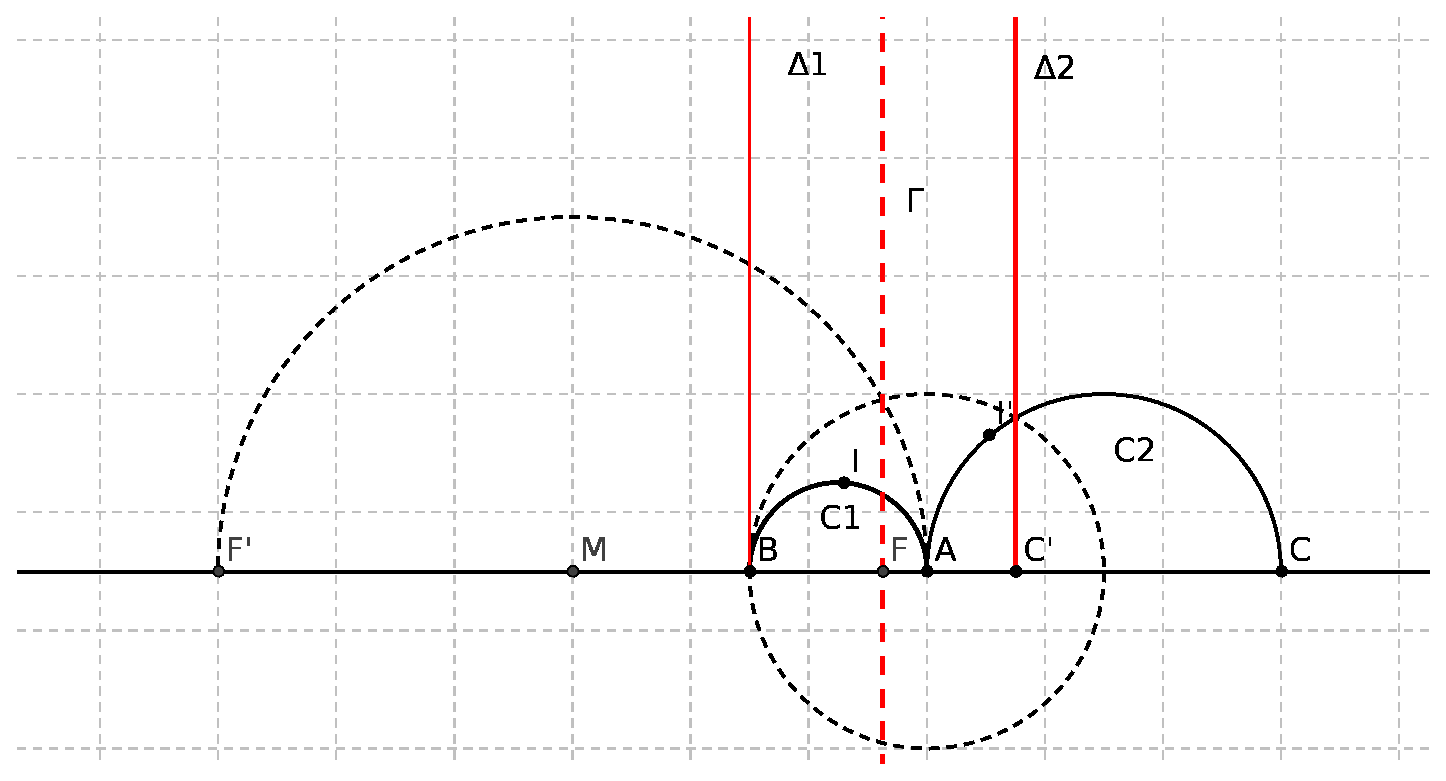
\includegraphics[scale=0.7]{figures/hyper37.eps}

\newpage 
\vspace*{\stretch{1}}
\begin{flushright}
\thispagestyle{empty}
\textit{...On n'écrit pas pour soi, on n'écrit pas pour les autres, on écrit aux autres, bien qu'on ne sache pas exactement à qui...}\\

Pierre Reverdy.

\end{flushright}
\vspace*{\stretch{2}}

\frontmatter

\part{Avant propos}

Ce livre se compose de trois chapitres.\\

Le premier est un historique rapide de la géométrie: on essaie de montrer pourquoi la naissance des géométries non euclidiennes a été aussi longue et difficile malgré la qualité des savants qui se sont intéressés au problème. Cette partie est accessible à tous.\\

Dans le second chapitre, on détaille les approches d'un certain nombre de mathématiciens. On le fait avec les connaissances qu'ils pouvaient avoir à leur époque, c'est-à-dire, celles qui sont données dans les Eléments d'Euclide. C'est pour cela que ce chapitre commence par l'énoncé des postulats ou axiomes utiles et celui des théorèmes d'Euclide qui seront utilisés ainsi que certaines de leurs démonstrations lorsqu'elles présentent un manque ou un problème.\

Cette partie peut s'adresser à tout le monde mais elle demande un effort important. Si les connaissances demandées en géométrie sont élémentaires (un élève de troisième les a!), il faut s'efforcer de raisonner en n'utilisant que les théorèmes auxquels on a droit. Il faut renoncer  à ce qui nous semble évident. Par exemple, dans certains cas un quadrilatère pourra avoir trois angles droits sans être un rectangle, ou alors par deux points distincts pourront passer plusieurs droites, etc...\

Enfin toutes les figures tracées le sont comme si on était dans le cadre euclidien, alors qu'on ne le sera pas! \\

Le troisième chapitre peut être lu par tous ceux qui ont des connaissances sur les nombres complexes, la structure de groupe et  les fonctions holomorphes ou le calcul intégral. Une des conclusions sera que le parallélisme n'est...pas toujours  une propriété essentielle.  

  
\tableofcontents

\mainmatter


\part{HISTORIQUE RAPIDE.}


                                                                                                                                                                                                                                                                                                                                                                                                                                                                                                                                                                                                                                                                                                                                                                                                                                                                                                                                                                                                                                                                                                                                                                                                                                                                                                                                                                                                                                                                                                                                                                                                                                                                                                                                                                                                                                                                           
                                                                                                                                                                                                                                                                                                                                                                                                                                                                                                                                                                                                                                                                                                                                                                                                                                                                                                                                                                                                                                                                                                                                                                                                                                                                                                                                                                                                                                                                                                                                                                                                                                                                                                                                                                                                                                                                             \chapter{Introduction:}
                                                                                                                                                                                                                                                                                                                                                                                                                                                                                                                                                                                                                                                                                                                                                                                                                                                                                                                                                                                                                                                                                                                                                                                                                                                                                                                                                                                                                                                                                                                                                                                                                                                                                                                                                                                                                                                                            
                                                                                                                                                                                                                                                                                                                                                                                                                                                                                                                                                                                                                                                                                                                                                                                                                                                                                                                                                                                                                                                                                                                                                                                                                                                                                                                                                                                                                                                                                                                                                                                                                                                                                                                                                                                                                                                                            
                                                                                                                                                                                                                                                                                                                                                                                                                                                                                                                                                                                                                                                                                                                                                                                                                                                                                                                                                                                                                                                                                                                                                                                                                                                                                                                                                                                                                                                                                                                                                                                                                                                                                                                                                                                                                                                                            
                                                                                                                                                                                                                                                                                                                                                                                                                                                                                                                                                                                                                                                                                                                                                                                                                                                                                                                                                                                                                                                                                                                                                                                                                                                                                                                                                                                                                                                                                                                                                                                                                                                                                                                                                                                                                                                                            
                                                                                                                                                                                                                                                                                                                                                                                                                                                                                                                                                                                                                                                                                                                                                                                                                                                                                                                                                                                                                                                                                                                                                                                                                                                                                                                                                                                                                                                                                                                                                                                                                                                                                                                                                                                                                                                                            
   Géométrie étymologiquement signifie mesure de la terre. Donc au départ la géométrie repose sur l'intuition que nous avons des objets qui nous entourent: droites, cercles, triangles et toutes les figures que l'on peut construire à partir de là. Le rôle du mathématicien sera de définir, d'ordonner, de démontrer, de dépasser notre intuition, nos sens qui, chacun le sait, peuvent facilement nous induire en erreur.\bigskip 
   
      L'histoire de la géométrie et plus généralement celle des mathématiques est liée à l'étude de leur lien avec ce que l'on appelle le réel, réel qui est une notion pas facile à définir et qui évolue avec nos connaissances!.\bigskip 
    
   Chacun d'entre nous est familiarisé avec la géométrie qu'on appelle euclidienne(GE). Elle correspond à notre environnement immédiat: formes géométriques usuelles, droites parallèles et perpendiculaires, longueur, surface, etc...                                                                                                                                                                                                                                                                                                                                                                                                                                                                   \bigskip 

    Et nous avons la certitude que, par un point, il passe une et une  seule droite parallèle à une droite donnée. Cette certitude est équivalente au cinquième postulat d'Euclide sur lequel nous reviendrons naturellement. Nous le nommerons P5. Nous réfléchirons aussi au sens qu'il faut donner à "postulat". Quelle différence y a-t-il avec "axiome"? \
     
     
    On peut démontrer que P5 est encore équivalent à l'énoncé: dans un triangle la somme des angles est égale à 180 degrés.\
    
    P5 occupe une place particulière chez Euclide (nous verrons en quoi plus loin). C'est un postulat donc un énoncé dont on ne sait s'il est démontrable ou non. Les mathématiciens, pendant des siècles, vont s'efforcer de le démontrer.\\
    
       
    

  Les géométries non euclidiennes (GNE) nient cette proposition . Ainsi on va affirmer soit qu'il n'existe aucune droite parallèle à une autre, soit au contraire que, par un point, il  existe une ou plusieurs droites parallèles à une droite donnée ou encore dans un triangle la somme des angles est inférieure ou supérieure à 180 degrés . Avouons que cela sort de notre compréhension immédiate et surtout de notre intuition. Et... on peut demander à quoi cela sert  de remettre en cause des choses qui nous semblent tellement vraies. \\
  

  Pourquoi ces nouvelles géométries? Pourquoi leur découverte est-elle      ex- -traordinaire ou importante? Pourquoi ont elles été rejetées avec tant de virulence et violence par des esprits parfois très brillants? Si Galilée, en remettant en cause la cosmologie aristotélicienne, a bouleversé au XVIIe notre appréhension de l'univers et donc la place de l'être humain, en quoi l'existence d'autres géométries possibles que celle dans laquelle on baigne en permanence transforme notre vision du réel?\bigskip 

   Aborder ces questions est une occasion de réfléchir sur les mathématiques, tout en en faisant, d'expliciter leur relation avec les autres savoirs et d'étudier la naissance d'une idée: comment elle apparaît, pourquoi à une certaine époque et pas auparavant? Pourquoi pendant plus de deux mille ans on va tourner autour sans avancer? Qu'est-ce qu'une théorie mathématique vraie?
\bigskip 

   Pour tenter d'apporter quelques réponses il faut se plonger dans les mathématiques grecques et plus généralement dans les connaissances des grecs, établir certaines liaisons entre mathématiques et autres savoirs, s'intéresser aux différentes tentatives faites aux différentes époques pour démontrer P5.\bigskip 
   
   Se lancer dans une aventure c'est sortir de ses certitudes. En cela, la découverte d'autres géométries est une aventure et on va voir que ce n'est pas facile! 
   
\chapter{Mathématiques grecques}

Qu'est-ce que les mathématiques? On pourrait passer des années à tenter d'en trouver une définition! D'autant plus que leur définition évolue avec les découvertes que l'on y fait. Mais n'est-ce pas la même chose avec les autres savoirs? Qu'est-ce que la littérature, la philosophie, l'art? etc...

\section{Naissance des mathématiques:}



    Certains font  naître les mathématiques avec Thalès au VIIe siècle  avant J.C. Pourtant on sait que les Babyloniens avaient déjà en -1750 des connaissances précises des grandeurs numériques: ils savaient par exemple que $119^{2}+120^{2}=169^{2}$ ou encore avaient conçu un algorithme capable de leur donner une approximation de $\sqrt{2}$ (1). Ils avaient en outre une bonne connaissance des calculs .\
     
     Quant aux Egyptiens ils faisaient aussi de la géométrie bien avant Thalès!\ 
   
   
   Alors pourquoi parler de Thalès? Parce que les grecs seraient les premiers à avoir tenté de  construire  avec rigueur des mathématiques en dépassant le stade de l'évidence.


  
  \footnote{(1) M.Caveing: Irrationalité dans les mathématiques grecques jusqu'à Euclide} 
  
  
  Les Grecs seraient les premiers à regarder les objets géométriques en tentant de les abstraire du monde physique. Ils les définissent abstraitement et leur attribuent des propriétés initiales évidentes. A partir de là ils énoncent des propriétés qu'ils démontrent logiquement.

      Mais ne pourrait-on pas constater que, lorsque que des hommes fondent une
communauté, ils abordent beaucoup de savoirs simultanément? Ne font-ils pas des mathématiques dès qu'ils ont besoin de se dénombrer, recenser leurs biens, prévoir l'avenir? Ne font-ils pas de l'histoire dès qu'ils apprennent à leurs enfants le passé du groupe? N'ont-ils pas dès le départ des activités artistiques à travers leurs chants, leurs contes, les bijoux, leurs outils? En fait dater la naissance d'un savoir est toujours difficile et arbitraire, d'autant plus qu'il est difficile d'en donner une définition.  C'est le cas des mathématiques.\

Vouloir dater la naissance d'un savoir n'est-ce pas finalement prétendre dater la naissance de l'humanité?\



     Ce que l'on peut affirmer c'est que les mathématiques grecques se développent dès le VIe siècle avant J.C. considérablement...mais comme tous les autres savoirs: l'histoire avec Thucydide, la tragédie avec Sophocle, la comédie avec Aristophane, la philosophie avec Platon et surtout le passage à l'écrit est déterminant!\\
     

      Au VIe siècle avant J.C les mathématiques se construisent comme une conception mathématique de l'univers: le nombre est une quantité discrète, c'est-à dire un multiple entier de l'unité (1) et inversement toute grandeur continue (ligne, surface, solide,...) peut être identifiée à un nombre, à un nombre entier qui la mesure ou à un rapport entre deux nombres: dans cette conception tout est nombre ou rapport entre deux nombres!  L'univers se décrit donc avec des nombres. C'est la conception des pythagoriciens.\\
      
       Les Grecs ne considérant (2) comme nombres que les nombres entiers cette conception sera remise en cause avec la découverte des grandeurs que nous appelons aujourd'hui nombres irrationnels (3). (Les mathématiciens avaient ainsi inventé au Ve avant J.C. un objet mathématique qui ne rentrait pas dans leur système de pensée).\
       
        \section{Quatre siècles de réflexion...:}
     
      
     
      La synthèse des mathématiques grecques est réalisée par Euclide au début du troisième siècle avant J.C.. Mais cette synthèse est le résultat des travaux des mathématiciens ou philosophes qui non seulement ont fait progresser les connaissances mais aussi ont réfléchi à leur lien avec le monde réel, problème qui est posé encore aujourd'hui! Nous développerons un peu plus loin ce point.\bigskip 
      
      \footnote{(1) pour les grecs les seuls nombres sont les nombres que nous appelons nombres entiers, donc 2,3,4,5, etc.. on peut remarquer qu'il n'y a pas 0 et 1 : 0 n'existe pas encore  et 1 n'est pas considéré comme un nombre: il est celui qui engendre les nombres.
      
      (2) Il s'agit de la première tentative de numérisation !  Aujourd'hui on essaie de tout numériser : le son, les images et même les émotions !La connaissance du cerveau commence  par là. \bigskip
   
    (3) On appelle, aujourd'hui, nombre irrationnel tout nombre qui ne peut pas  s'écrire sous la forme a/b, a et b entiers.
    Pour les pythagoriciens de même que tout nombre est un multiple de l'unité, deux grandeurs doivent être commensurables c'est à dire multiples entières de la même unité, ce qui n'est pas le cas pour la diagonale du carré et l'un de ses côtés.  
     Rappelons que si le côté d'un carré est égale à 1 sa diagonale est $\sqrt{2}$ dont on démontre qu'il n'est pas rationnel. Euclide (et Aristote avant lui)  propose une démonstration.} 
      
    
      
      \newpage 
       \chapter{Eléments d'Euclide}
  \section{introduction}
  
   Les Grecs mettront quatre siècles à construire les Eléments d'Euclide. Ils sont le résultat de la réflexion de Thalès, Pythagore, Platon, Aristote et de tous ceux qui entourent ces grands penseurs.\\
   
    Euclide aura le mérite de réaliser la synthèse de ces travaux, au début du troisième siècle avant J.C. Cette synthèse
   représentera pendant 2000 ans l'oeuvre de référence des mathématiques. On ne sait pas grand chose d'Euclide, si ce n'est qu'il vivait à Alexandrie. Il n'était sans doute pas tout seul à rédiger ce travail.\\
       
       
      Même si les arabes ont apporté au Moyen Age beaucoup de connaissances, ce n'est qu'avec l'émergence, de ce que l'on appelle aujourd'hui "analyse" (1) avec Newton, Euler, Laplace,etc...,  que les Eléments d'Euclide seront remis en cause, en tant que synthèse.\bigskip 
   
   Montucla (2), à la fin du XVIIIe, affirme qu'Euclide "mit dans son livre cet enchaînement si admiré par les amateurs de la rigueur géométrique...En vain, divers géomètres, à qui cet arrangement a déplu ont tâché de le réformer. Leurs efforts impuissants ont fait voir combien il était difficile de substituer à la chaîne formée par le géomètre grec une autre aussi ferme et aussi solide". 

  
 Même si ce jugement sera discuté dans les siècles suivants il montre à quel point  les éléments d'Euclide auront été importants et auront imprégné tous les mathématiciens ou les philosophes jusqu'au XVIIe siècle.\\
 
 Autre citation, mais celle-ci du XXe,: au début des Eléments de Nicolas Bourbaki (3), on trouve cette phrase: " ce qui était une démonstration pour Euclide en est toujours une à nos yeux".\   


  

   
    \footnote{(1) le mot analyse est créé pour s'opposer aux Eléments d'Euclide qui étaient considérés comme la synthèse des mathématiques et pour montrer que les nouvelles mathématiques ne pourraient pas s'y intégrer.
    
  (2) Montucla est peut-être le premier historien des mathématiques et a publié son histoire des mathématiques en 1793.
  
  (3) Nicolas Bourbaki est en fait un groupe de grands mathématiciens, français en général, qui ont voulu rédiger les mathématiques du XXesiècle. Ils ont constitué une école qui a dominé les mathématiques pendant au moins un demi siècle. \
  
    }  
  
 

 
 
 \newpage  \section{Composition des Eléments d'Euclide:}
  
    
    
    Les éléments d'Euclide sont composés de treize livres:\
    
  
  
  
 
 
     

  
 
 
 

    Les quatre premiers livres traitent de la géométrie plane. Mais un certain nombre de théorèmes peuvent être traduits en utilisant l'algèbre d'aujourd'hui et, par exemple,  la proposition 4 du livre 2 permet de résoudre une équation du second degré.\
   
   
   Le livre 5 est un gros livre qui traite des proportions. Ses résultats vont être appliqués à la géométrie plane dans le livre 6. \
   
   
  Les trois livres suivants forment un traité d'arithmétique dans lequel on démontre  beaucoup des propriétés qu'apprennent nos lycéens d'aujourd'hui.\
  
  
  Le livre 10 traite des grandeurs incommensurables que, de nos jours, nous appellerions irrationnelles.\
  
  
   Les livres 11 et 13  traitent la géométrie de l'espace.\
   
   
   Le livre 12 nous parle des aires curvilignes en les comparant aux aires des polygones par la méthode d'exhaustion. 
   
    L'ensemble est d'une très grande rigueur,  parfaitement ordonné et d'une grande cohérence. On y sent la présence des philosophes ou mathématiciens, que ce soit Aristote ou Platon (1) ou d'autres.
 
    Le livre qui nous intéresse particulièrement ici est le premier.\\

  \section{Composition du livre 1:}\
  
  
     Il y a d'abord 35 définitions ensuite 6 postulats et 9 axiomes, enfin 48 théorèmes.
    Il faut passer un peu de temps sur chacun des mots: définition, postulat et axiome.
  Aristote un siècle plus tôt  a posé les bases de la logique. Euclide va les utiliser.\\
  
  \subsection{Les axiomes ou "notions communes":}
  

  Il y a neuf axiomes que les grecs dénomment  "notions communes" Il s'agit de propositions dont on aura besoin et dont on affirme qu'elles sont indémontrables et vraies: on ne peut pas les remettre en cause. Ces notions communes s'appliquent à toutes les grandeurs quelles qu'elles soient, numériques, géométriques ou non.\\
  
   
  \begin{footnotesize}
  
  
  ( 1) Platon définit parfaitement le travail du mathématicien (quelle que soit l'époque!) dans République (IV 510 c et d). Une démonstration se déroule est une suite d'opérations, définies par des règles, qui permettent de passer d'une affirmation à une autre. 
   Il indique, en particulier, que la figure que l'on trace n'est que l'image d'une figure parfaite, abstraite, que l'on ne peut appréhender que par la pensée.
  \end{footnotesize}
  
   
\newpage 
  
  
 Par exemple, le dernier axiome est: "Le tout est plus grand que la partie". Ceci est faux dans les ensembles infinis mais vrai dans les ensembles finis. Chez les Grecs toute chose est finie. L'infini n'existe pas ou tout du moins dans notre sens. C'est un sujet traité abondamment par les philosophes grecs (1). C'est un problème essentiel dans les éléments d'Euclide.\\
 
 \subsection{Les postulats ou "demandes":}
      
    Il y a six postulats: postulat vient du latin postulatum qui signifie "demande". Il s'agit de propositions, s'appliquant à des objets géométriques, dont on aura besoin par la suite pour démontrer des théorèmes . Quel est le statut du postulat par rapport à l'axiome? la réponse n'est pas évidente et fera l'objet au cours des siècles de longs débats.

   Donnons deux exemples:\
   
    La première demande est "de pouvoir joindre tout point donné à tout autre point donné par une ligne droite". Est-ce un théorème? Et dans ce cas faudra-t-il le démontrer? La question est ouverte. Au départ il nous permettra d'affirmer l'existence d'une droite joignant deux points.\\
   
 
    Le cinquième postulat est le fameux P5: si une droite, tombant sur deux droites, fait les angles intérieurs du même côté plus petits que deux droits, ces deux droites prolongées indéfiniment, se rencontreront du côté où les angles sont plus petits que deux droits. (cf fig 1).\\ 
    
     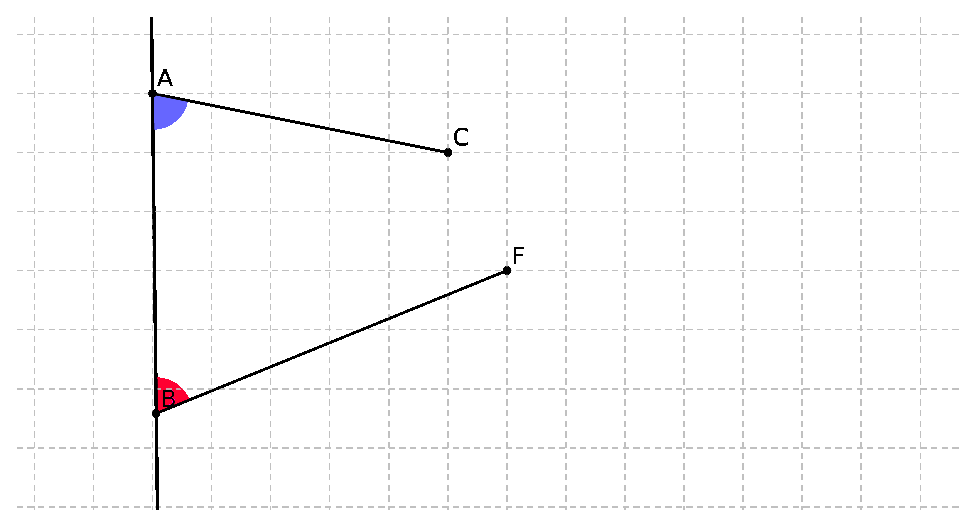
\includegraphics[scale=0.7]{figures/euc1.eps} \\
    
    
\begin{footnotesize}
(1) Chez Aristote, dans les livres de la \textit{Physique}, on traite de l'infini: c'est une notion liée à l'étude du mouvement. \

" Le nombre est infini en puissance mais pas en acte"(207 b): ce qui signifie que l'on ne peut pas parler de l'ensemble de tous les nombres mais quel que soit un nombre on peut en trouver un plus grand.\

"il n'y a pas de grandeur sensible qui soit infinie, il ne peut y avoir de grandeur qui dépasse toute grandeur déterminée, car ce serait une chose plus grande que le ciel"(207 b) 
\end{footnotesize}
    
 
   
   
   
   
   
    \newpage Expliquons la figure: les droites (AC) et (BF) coupent une même droite en faisant des angles, CAB et FBA, dont la somme est inférieure à 180 degrés. P5 nous dit alors que les droites prolongées se couperont. Nous parlerons des droites un peu plus loin.\\
    
    
    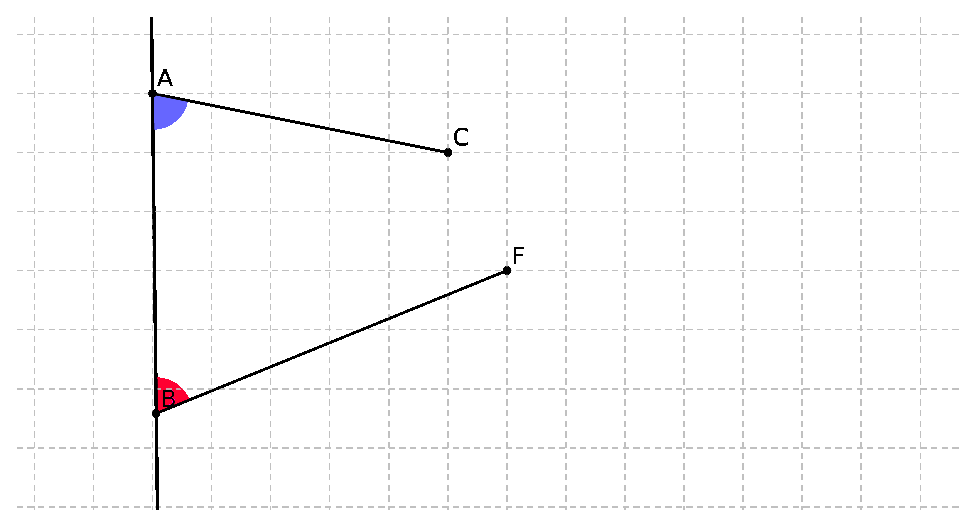
\includegraphics[scale=0.7]{figures/euc1.eps} \\
    
     
   
 
 
   Dans les Eléments d'Euclide, on décide, au départ, de ne pas démontrer P5 mais on décide, aussi, de ne pas le poser comme axiome. C'est ce postulat que les mathématiciens vont essayer, régulièrement, de démontrer pendant 2000 ans! soit en le remplaçant par un autre postulat, soit en le supprimant et en modifiant la définition du parallélisme soit en raisonnant par l'absurde, c'est-à dire, en supposant que P5 est faux. \
   
 Ce postulat a posé un problème dès le départ.\
 
   
  On peut noter la formulation compliquée de ce postulat, formulation qui, d'après certains, ressemblerait à un théorème!\
  
   C'est un résultat que l'on ne peut pas vérifier expérimentalement car il s'agit d'un passage à la limite: plus la somme des angles se rapproche de 180 degrés et plus le point d'interchapter des droites "s'éloigne".\bigskip 
  
   La composition même du livre 1 nous interroge: Les vingt-huit premiers théorèmes ne l'utilisent pas. Et on va s'en servir pour démontrer les propriétés du parallélogramme ou du rectangle, propriétés qui nous semblent évidentes et si proches du monde réel tel qu'on le conçoit.\
   
   Enfin il y a toujours cette question à laquelle il est difficile de répondre: qu'est-ce, exactement, qu'un postulat? \\
   
   Mais le rôle du mathématicien est bien d'aller au de se poser toutes les questions et de ne pas se laisser influencer par sa conception du monde physique. Son rôle, comme celui de l'artiste, est de nous sortir du réel que nous croyons connaître pour nous faire rentrer par un autre chemin dans un autre réel.\\
   
   
   
 \subsection{Les définitions:}
         

   Il y a  aussi des  définitions: plus généralement qu'est-ce qu'une définition? Il n'est pas facile de répondre!  Et pourtant c'est un problème fondamental: quel sens pourrait-on donner à une activité dont les objets d'étude ne seraient pas définis. C'est un problème permanent dans toute activité. Parmi les définitions les sept premières nous présentent les objets points, droites, surfaces planes. L'existence de ces objets est donnée à priori. Ce sont des termes primitifs que l'on ne discutera pas. Ils gardent un contenu intuitif et sont définis en termes de réalités physiques mais en même temps abstraits de la réalité physique.  \bigskip 
   
   
    Donnons un exemple: la première définition est "Le point est ce qui n'a pas de partie". Dans cette définition, le mot grec utilisé pour "point" est "sémaïon" qui signifie signe ou pointe du poinçon donc c'est une réalité physique que l'on peut diviser, découper... mais "est ce qui n'a pas de partie" nous fait sortir de cette réalité physique.  On est dans le monde des idées.  Mais on pourrait se demander aussi ce que signifie "partie"...

  Les autres définitions sont celles d'objets qui reposent toujours sur notre intuition mais dont on va parfois démontrer l'existence. Par exemple, le triangle équilatéral est celui dont les côtés sont superposables: on en démontrera l'existence dans le théorème 1 du livre 1.

     
  La dernière définition est celle du parallélisme de deux droites.\\
  

  Revenons sur la définition de la droite. La définition 2 nous dit qu'une ligne (donc une droite) "est ce qui a une longueur mais pas d'épaisseur".\bigskip
  
  Là aussi, s'il est possible de dessiner une ligne qui a une longueur, il est impossible de dessiner une ligne qui n'a pas d'épaisseur. Dans ce sens tout dessin géométrique n'est que la représentation d'une idée abstraite.\
   
  
    La définition 3 nous dit que "les extrémités d'une ligne sont des points".\bigskip 
    
   La définition 4 nous dit qu'une droite est "une ligne qui se couche de manière égale entre ses points". En d'autres termes, par deux points d'une droite passe une droite et une seule.\
   
   Faisons plusieurs remarques:\\ 
   
1. Une ligne n'est pas un ensemble de points. Seules ses extrémités sont des points. Une ligne, pour les Grecs, ne peut pas être, comme on le dit aujourd'hui, un ensemble infini de points pour plusieurs raisons. \

Tout d'abord, l'infini n'existe pas "en acte" pour les grecs, il est uniquement "potentiel" (cf Aristote: traité de physique) ce qui signifie, par exemple, que  l'on ne peut pas parler de l'ensemble de tous les nombres même si les grecs savent, naturellement, que quel que soit le nombre il en existe un plus grand. Pour la ligne c'est la même chose: on pourra prendre autant de points que l'on veut sur une ligne mais on ne pourra pas parler de l'ensemble des points de la ligne.\

Ensuite, pour arriver à considérer qu'une ligne est un ensemble infini de points, en mathématique,  il faut maîtriser mathématiquement la notion d'infini et construire l'ensemble des nombres que l'on appelle réels. Cela ne sera fait qu'à la fin du XIXe siècle.\\


2. Une ligne, comme toute figure, est finie. Un objet non fini, dans le sens où il n'aurait pas d'extrémités, serait non pas infini mais non défini, c'est à dire non connu; et on ne peut pas travailler sur un objet que l'on ne connaît pas!\bigskip 

Une dernière remarque sur les définitions:
 on a des définitions d'objets dont on démontrera l'existence (par exemple le triangle équilatéral) ou des définitions d'objets dont on admettra l'existence à priori (par exemple la droite) ou encore des définitions de mots (comme parallèle). Il y a donc des niveaux différents dans ces définitions. 
 
 \subsection{Les théorèmes:}
 
 Un théorème est un énoncé que l'on doit démontrer.\
 
 
 Dans le livre 1 il y a quarante huit théorèmes et on commence à utiliser P5 à partir du théorème 29.

  Euclide a donc démontré d'abord les théorèmes qui ne nécessitaient pas l'utilisation de P5. Il aurait pu procéder autrement. Une fois de plus P5 a un rôle particulier! 
    
  Cette construction résulte manifestement  d'une réflexion autour de P5.
  
  \subsection{Notion de distance:}
  
  Dans les Eléments d'Euclide on ne parle pas de distance. Par exemple, une droite est plus petite qu'une autre si étant ajustée à l'autre elle y est contenue. On ne parlera pas de sa longueur.\
  
  Il ne peut pas y avoir de distance: en effet, s'il y avait une notion de distance, on pourrait, dans l'espace, choisir un segment unité qui permettrait de mesurer n'importe quel segment.\
  
   Mais le carré qui aurait comme côté ce segment unité aurait une diagonale qui  ne pourrait pas s'exprimer "rationnellement", c'est à dire qui ne serait pas un fraction de deux nombres entiers. Donc, ne pouvant pas associer à la diagonale de ce carré un nombre celle-ci n'aurait pas de longueur! Et les Grecs avant Euclide connaissaient ce résultat.\
  
  Euclide surmonte ce problème en définissant la notion de "commensurabilité" ou d'"incommensurabilité", ce qui n'est pas facile mais efficace car il peut démontrer plein de résultats, en particulier, dans le livre 13 il démontre l'existence des cinq solides réguliers (1)(cf \textit{Timée} de Platon).\\
  
   \begin{footnotesize}
   (1) Voici les cinq solides réguliers de Platon: tétraèdre( quatre faces équilatérales), cube( six faces carrées), octaèdre(huit faces équilatérales), dodécaèdre(douze faces pentagonales régulières), icosaèdre(vingt faces équilatérales).
   \end{footnotesize}\\

\newpage \subsection{Conclusion:}

L'objectif d'Euclide va être de démontrer ses théorèmes seulement à partir de ses définitions, demandes et axiomes. \

Cependant les figures qui accompagnent les démonstrations vont parfois servir d'arguments de démonstration. Par exemple, dans la démonstration du théorème 17 du livre III, il admet qu'une droite joignant deux points, l'un à l'intérieur d'un cercle et l'autre à l'extérieur, coupe le cercle, simplement par l'observation de la figure. On est loin des exigences de Platon ou d'Aristote qui ont la volonté de ne jamais rien admettre sans démonstration. 
   Il est étonnant de voir que cette exigence va s'estomper au cours des siècles et que l'on va considérer qu'il y a une parfaite harmonie entre  les objets géométriques et leurs images visibles  ou  proclamer la "vérité évidente" des axiomes de la géométrie. \\
   
  
   
 
 Mais les figures peuvent parfois n'être que l'illustration d'une idée. Par exemple dans le livre V on démontre des théorèmes sur les relations entre les grandeurs. Ces grandeurs sont toujours représentées par des droites et les démonstrations apparaissent en première lecture comme des exercices de géométrie sur des droites et pourtant dans le livre VI dans la démonstration du théorème 2 (Thalès) on utilise un théorème du livre V et cette fois les grandeurs seront des triangles. Ces figures géométriques ne sont donc parfois que la représentation d'idées.\\
   
   Les Eléments d'Euclide présentent des insuffisances, mais l'ensemble est tellement fort que l'on peut comprendre pourquoi pendant deux mille ans ils ont été la référence incontournable des mathématiciens et du raisonnement en général.\
   
Et ce n'est pas un hasard si encore aujourd'hui,  ils sont aussi étudiés.\\

 
   
  
  Une remarque pour terminer: on ne trouve pas une fois le mot géométrie dans les élément d'Euclide! En fait un géomètre n'est pas dans l'Antiquité un mathématicien. Il est celui qui fait des relevés de terrain: c'est un technicien. Il n'est pas dans le monde des idées.\bigskip 
  
   

  
 

 

  
 
 
  
  
    
 
\newpage  
\chapter{Mathématiques et monde réel}

\section{Mathématiques fondamentales et appliquées:}
\textit{
« M. Fourier avait l’opinion que le but principal des mathématiques était l’utilité publique et l’explication des phénomènes naturels ; mais un philosophe comme lui aurait dû savoir que le but unique de la science, c’est l’honneur de l’esprit humain, et que sous ce titre, une question de nombres vaut autant qu’une question du système du monde. » }

\textit{C.Jacobi (mathématicien allemand) dans une Lettre à Legendre, 1830}.\\


Les mathématiques se développent à la fois indépendamment des autres savoirs et en liaison avec eux. On parle souvent de mathématiques fondamentales et de mathématiques appliquées comme étant opposées mais cette distinction est une erreur car ce sont toujours des mathématiques (1). On peut simplement dire que des théories mathématiques ont été créées à partir de problèmes du quotidien tels que, le dénombrement d'une population, l'écoulement d'un fluide ou les flux financiers, etc... ou d'autres théories telles que les  probabilités de Pascal, le calcul différentiel de Leibniz, la théorie des ensembles ou encore... les géométries non euclidiennes qui auront été créées uniquement grâce à la curiosité ou pour l'honneur de l'esprit humain. \\



  \footnote{
 (1) Une différence cependant entre les deux types de théories: les "fondamentales" sont beaucoup moins financées que les "appliquées"... les décideurs politiques ou économiques n'étant pas toujours des visionnaires! Et pourtant les mathématiques fondamentales peuvent avoir des applications essentielles pour la société!}\
 

  
  
  
 \newpage \section{De l'antiquité à nos jours:}
 

 
 
 Aristote n'a pas écrit de traité de mathématiques mais il en parle un peu...partout! et en particulier de leur rapport avec la physique. \
 
 Par exemple dans \textit{Physique II 193b-194a} Aristote montre le lien et les différences entre la physique  et les mathématiques: "...appartiennent aux corps physiques les surfaces, solides, grandeurs et points qui sont l'objet des études mathématiques" et plus loin "il appartient au physicien de connaître l'essence du soleil et de la lune mais aussi de leurs attributs essentiels...attributs objets d'étude des mathématiciens". Plus loin encore "la géométrie étudie la ligne physique en tant qu'elle n'est pas physique; au contraire l'optique étudie la ligne mathématique, non pas en tant que mathématique, mais en tant que physique".\\
 

Dans \textit{Métaphysique I, 989 b}, Aristote affirme, dans sa critique des pythagoriciens, que "les êtres mathématiques sont privés de mouvement, à l'exception de ceux dont traite l'Astronomie." Donc, pour lui, la géométrie est une science qui porte sur des objets qui échappent au mouvement alors que la physique a pour objet l'étude du mouvement.\
 
 Si  la physique et les mathématiques peuvent s'apporter des informations, en aucun cas les mathématiques ne permettront d'expliquer les phénomènes naturels.\\
 


 
 
 
 Pour Aristote les mathématiques ne peuvent donc pas être utilisées pour comprendre le réel: par exemple la sphère mathématique n'existe pas physiquement, c'est une idée. Galilée (1) va lui répondre que, si la sphère n'existe pas, tout caillou a une forme géométrique, peut être unique mais géométrique quand même. \
 
Galilée  arrive au moment où la physique d'Aristote est de moins en moins satisfaisante: les observations astronomiques sont de plus en plus précises, l'explication du mouvement des planètes devient de plus en plus compliquée et  Copernic montre que l'héliocentrisme répond mieux au mouvement des astres. De plus on est toujours incapable de comprendre le mouvement d'un objet qu'on lance: comment expliquer ce le mouvement de la pierre au moment où elle  sort de la main? \\
  
  
  
  
  \footnote{ 
  
  (1) Le  "Dialogue sur les deux plus grands systèmes du monde" est l'ouvrage de Galilée dans lequel il expose sa vision du cosmos. On notera qu'il l'a écrit en italien alors que tous les ouvrages scientifiques de l'époque le sont en latin. 

  Trois personnages interviennent:
  Salviati qui représente Galilée.
  Sagredo un personnage éclairé mais sans a priori qui sera convaincu par Salviati à la fin du dialogue.
  Simplicio un personnage pas très intelligent défendant la thèse géocentrique, c'est à dire celle de l'Eglise. (Le pape se reconnaîtra dans Simplicio et ne sera pas très content...)
  Galilée se fera condamner par l'Inquisition et préfèrera se rétracter plutôt que de brûler sur le bûcher...}
  
  
  
  
 
 
   
 
  \newpage Galilée va affirmer que pour comprendre la nature il faut suivre "le chemin de la simplicité". La physique d'Aristote est trop compliquée. Et le chemin de la simplicité passe par la géométrisation du monde physique et en l'idéalisant il va créer la physique moderne. \
  Newton poursuivra dans cette voie et expliquera pourquoi, par exemple, la lune tourne autour de la terre.\\
  
  
  Aujourd'hui il est évident  que la technologie utilise les théories mathématiques les plus abstraites, en particulier la numérisation des phénomènes physiques. Mais il faut avoir en permanence à l'esprit qu'un modèle mathématique appliqué à une réalité est une idéalisation de cette réalité et donc n'en est qu'une approximation. Et l'oublier peut conduire à un...crash boursier.\\
  

   Rajoutons que la géométrie, euclidienne ou non, a un lien avec la réalité, avec l’espace réel . C’est cette position  que soutient Einstein (1) dans "géométrie pure" et "géométrie appliquée". Pour lui, à l’origine, on a fait de la géométrie pour décrire le comportement des phénomènes physiques; c’est bien ce à quoi elle sert chez Newton. Ainsi, chez ce dernier, notre espace ou les objets dans l’espace réel, obéissent réellement aux lois de la géométrie euclidienne. \bigskip
   
    Certains, au XIXe, se sont même demandés si la géométrie faisait partie des mathématiques, si elle n'était pas qu'une théorie physique, qu'un outil ou encore l'expression de la théorie de Newton. Mais alors, si le postulat V d'Euclide n'est pas démontrable, si ce n'est qu'une hypothèse, les lois de Newton ne pourraient être, peut-être, que des hypothèses, ce qu'au XIXème on refuse.   \\
    
      Et c'est Hilbert qui, en 1899, dans son livre, \textit{"Fondements de la géométrie"}, démontrera que la géométrie, qu'elle soit euclidienne ou non, est bien une activité mathématique comme une autre.\\
   
   \footnote{(1) Dans son article de 1921 \textit{La géométrie et l'expérience}, Einstein affirme une séparation très nette entre les mathématiques, qui ne peuvent pas s'appliquer au réel, et leurs applications qui font partie intégrante de la réalité.b\
  
  Il énonce, en particulier, cette proposition: \textit{« Pour autant que les propositions 
des Mathématiques se rapportent à la réalité, elles ne sont pas certaines, et pour 
autant qu'elles sont certaines, elles ne se rapportent pas à la réalité. »}}
  
 
  \newpage Les mathématiques sont liées aux autres savoirs et c'est pour cela qu'elles se développent mais c'est aussi pour cela que leur développement peut être freiné! Nous le verrons! Ce que l'on peut affirmer, de toute façon, c'est que les mathématiques se développent d'autant plus que les autres savoirs s'enrichissent.
   \bigskip
   
  
  
  
  
   

  
  Aujourd'hui on continue à étudier le lien des mathématiques avec les autres disciplines, mais plus seulement la physique: l'économie, la biologie, etc...Pour résumer, on pourrait dire que le mathématicien a les pieds dans la terre et la tête dans les étoiles...
  
   Plusieurs types d'activités auraient pu contribuer à la mise en place des géométries non euclidiennes: la philosophie, la géographie, l'astronomie et certaines activités artistiques telles la peinture, l'architecture ou la musique.

  \newpage  
  
     \section{La géographie:}\
     
    
     
   
   
   
   Rappelons que "Géographie",
    signifie étymologiquement dessin ou écriture de la terre et  "géométrie" mesure de la terre. Les Grecs savent que la Terre est ronde et Eratostène (1) mesure son rayon. Celui-ci va  poser le problème de la cartographie: est-il possible de trouver une méthode capable de représenter une portion de sphère sur une surface plane, méthode qui respecterait les dimensions réelles? Les Grecs ne résoudront pas ce problème (2) mais ils ont bien conscience que lorsqu'ils tracent une ligne sur le sol ce n'est jamais une droite! D'ailleurs dans les Eléments d'Euclide on parle d'angle curviligne.\
    
     Examinons un peu la géométrie sur la sphère.\\
    

  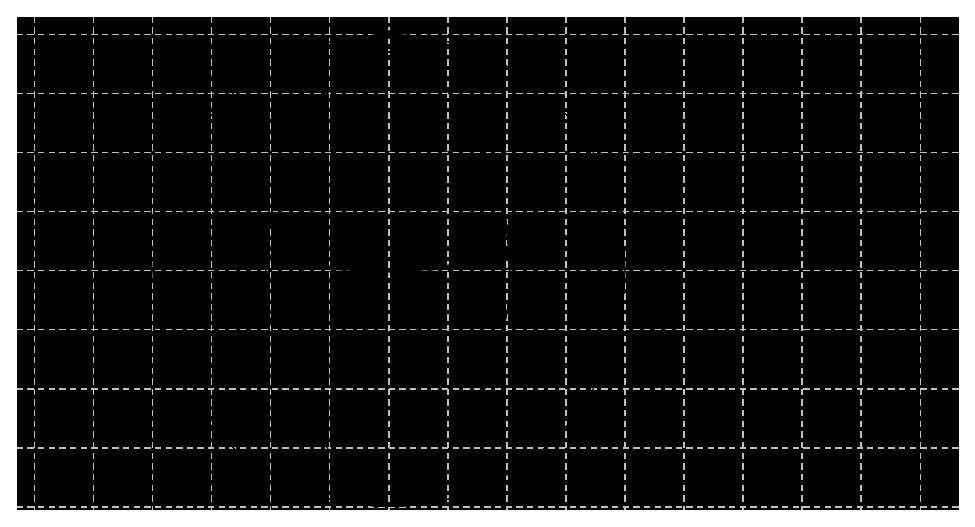
\includegraphics[scale=0.7]{figures/neuc.eps}\\
  
  
  Si on trace deux cercles passant par les deux pôles de la terre et la ligne de l'équateur, ces lignes définissent un triangle curviligne (cf figure 2) dont les angles à la base sont égaux à 90 degrés donc la somme des trois angles de ce triangle est supérieure à 180 degrés! Donc on n'est plus dans le cadre de la géométrie euclidienne: travailler sur une sphère conduit à d'autres conclusions. L'espace dans lequel on travaille joue un rôle fondamental.\\
 
  



  
  
   \footnote{(1) Eratosthène est né en -276 à Cyrène (aujourd'hui en Lybie). Il est spécialiste en...tout: philosophie, histoire, maths, etc...Il devient directeur de la bibliothèque d'Alexandrie qui a été le plus grand centre culturel de l'Antiquité.

(2) C'est Euler qui répondra en 1775 à cette question par la négative. Il faudra donc presque deux mille ans pour répondre à cette question. \

Euler est un des mathématiciens les plus prolifiques de tous les temps et qui  a écrit sur  tout. Par exemple il a élaboré un théorie musicale, a eu une correspondance avec Kant, etc...  }  
  
 \newpage
 

 
  
  
  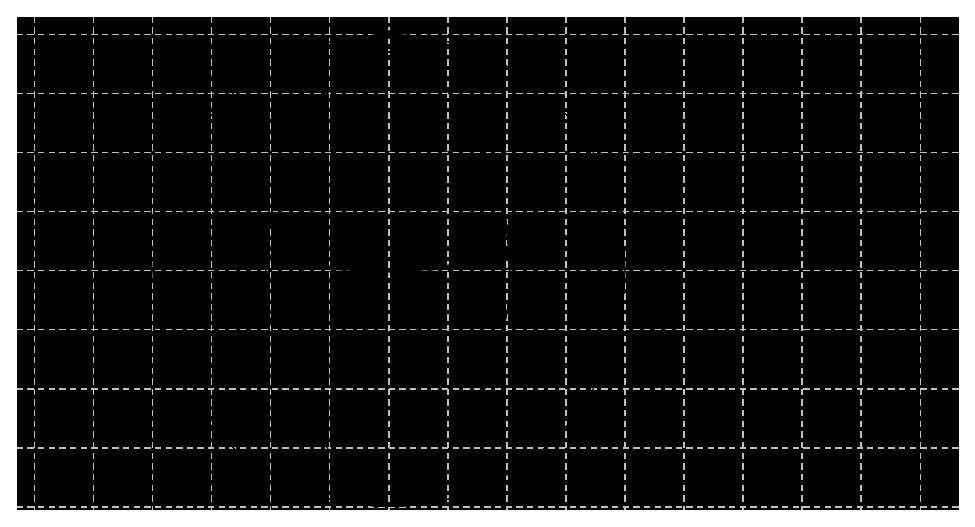
\includegraphics[scale=0.7]{figures/neuc.eps} 
  
  fig2:
  les méridiens EC et ED sont perpendiculaires entre eux et à l'équateur CD\\
  
  
  Cependant il y a des analogies entre la géométrie du plan et la géométrie d'une sphère. L'un des éléments essentiels des figures de la géométrie est la ligne appelée droite qui est caractérisée par le fait qu'elle est déterminée par deux quelconques de ses points, ce qui une conséquence à la fois  de la quatrième définition  et du sixième postulat du premier livre des Eléments d'Euclide.\
  
   
 
 Sur une sphère de rayon R, si on prend deux points, il passe un cercle de rayon R qu'on appellera géodésique (1) ou grand cercle. Chaque grand cercle est déterminé  par deux quelconques de ses points. Un grand cercle est l'équivalent sur la sphère de la ligne droite sur le plan. On peut alors construire les figures équivalentes à celle de la géométrie plane : triangles, quadrilatères, cercles, angles, etc.... Il suffit de remplacer dans les définitions du plan droite par grand cercle. \
 
 Mais l'analogie entre plan et sphère n'est pas complète! Tout d'abord il n'existe pas de grands cercles parallèles au sens d'Euclide, c'est à dire sans points communs et ensuite, si par  deux points non diamétralement opposés il existe un seul grand cercle, par deux points  diamétralement opposés il passe une infinité  de grands cercles. Alors que, dans le plan, par deux points distincts passe une droite et une seule. \\
    
    On peut noter que Théodose (IIe et Ier siècle av.J.C) et Menelaus(Ier siècle) ont créé une géométrie sphérique que Ptolémée (IIe siècle) va utiliser en astronomie. Puis les mathématiciens arabes vont développer ces travaux, en particulier, Al Khwarismi (XIe).\bigskip
    
    Ainsi faire de la géométrie sur une surface non plane aurait pu conduire à créer une autre géométrie. C'est cela que va faire Riemann à la fin du XIXe et créer ainsi une géométrie non euclidienne.(cf au chapitre suivant pour  le travail que l'on peut faire sur la sphère) \bigskip
 
 
 
    
  \footnote{ (1) On peut définir la notion de géodésique sur une surface quelconque munie d'une distance: une géodésique désigne la généralisation d'une ligne droite sur une surface. En particulier, le chemin le plus court, ou l'un des plus courts chemins s'il en existe plusieurs, entre deux  points d'une surface munie d'une distance est une géodésique. }   

 
   
    
   
    
    
   \newpage  \section{La peinture à la Rennaissance:}\
    
    
    
   
    
     Le problème est de représenter un objet de l'espace dans le plan tel qu'il est ou tel qu'on le voit: comment donner l'impression de profondeur?
   Si l'on se met à une fenêtre comment représenter sur une toile exactement ce que l'on voit? Quand on est au milieu d'une route dont les bords sont parallèles et que l'on  regarde le "bout" de la route on a l'impression que les bords se rejoignent.\
   
    Notons ABCD, le plan représentant la route, et EFGH le plan perpendiculaire passant par (EF) représentant la toile sur laquelle on veut représenter la route. L'oeil du peintre est en O. (figure ci-dessous).
 
  Pour décrire cette situation on invente ce que l'on appelle un point de fuite .
  
    
 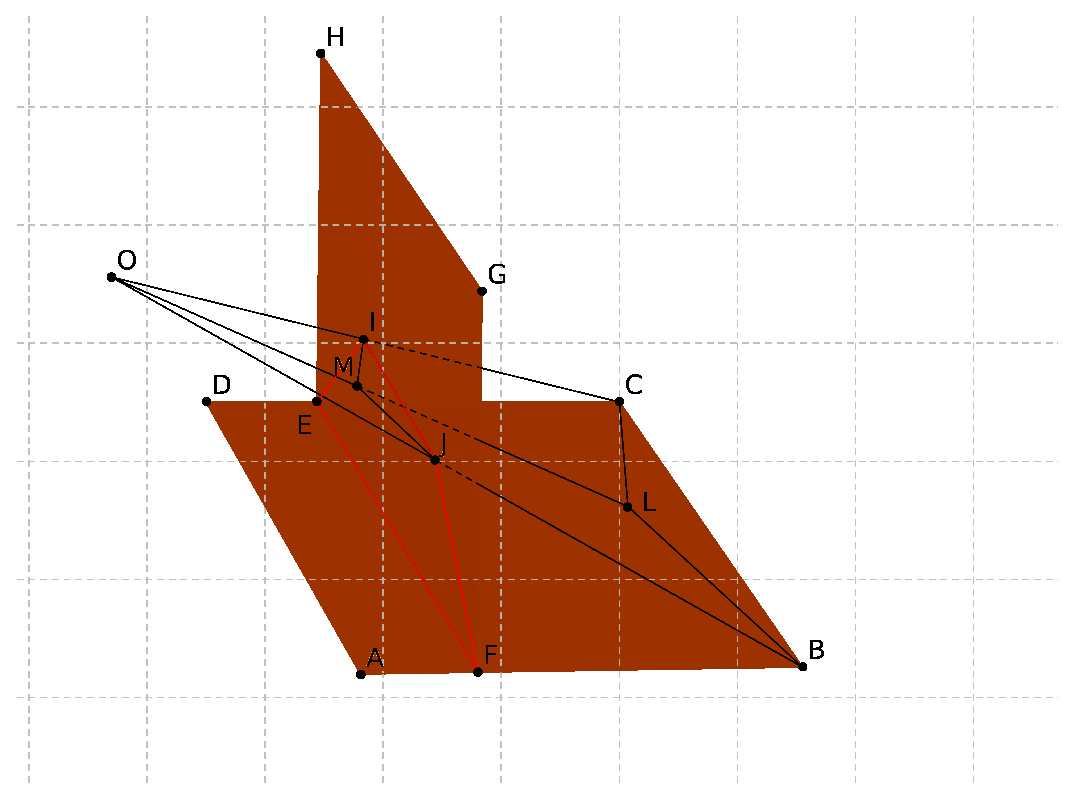
\includegraphics[scale=1]{figures/peint.eps} 
   
    
    Chaque fois que l'on regarde un point L de la route à partir de O, cela correspond au rayon lumineux OL qui coupera la toile en un certain point M. On dira que M est l'image de L sur la toile T.
 

 
  Ainsi  B aura pour image J et F aura pour image lui-même.\
  
  
 Toute droite joignant O à un point du segment [BF], bord de la route, coupera T en un point de [JF] et toute droite joignant O à un point du segment [CE] coupera T en un point de [EI]. Ainsi [BF] a pour image  [JF] et [CE] a pour image [EI]. \
 
  La portion de route EFBC sera donc représentée par le trapèze EFJI. C'est ainsi que le peintre verra la portion de route EFBC.\
  
  
   [JF] et [EI] se coupent en un point K. En fait si on regarde le bord FB, plus B s'éloigne de F et plus J se rapproche de K. De même, si on regarde le bord EC plus C s'éloigne de E et plus I se rapproche de K. Ainsi si je regarde "à l'infini", cela correspond à une droite horizontale partant de O et passant par K. \
   
 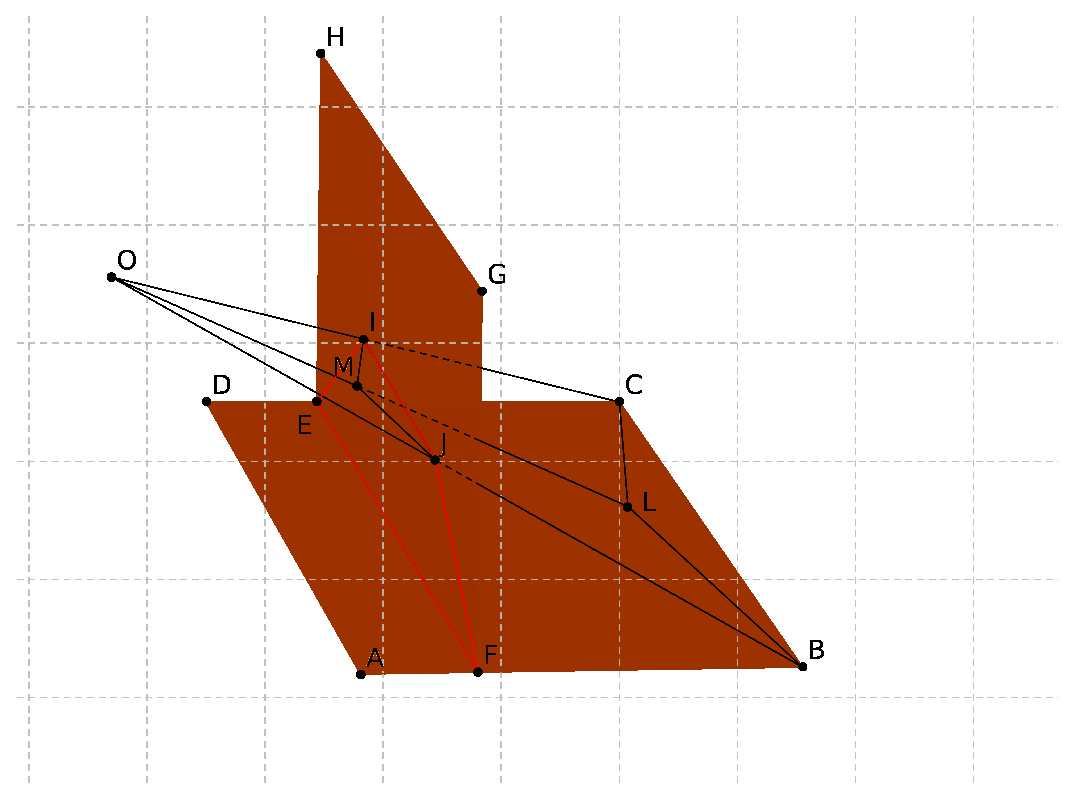
\includegraphics[scale=1]{figures/peint.eps} 
   
   

   On dira que K est l'image du point à l'infini des deux bords de la route que l'on voit se rejoindre, comme si deux droites parallèles se coupaient à l'infini. Effectivement, c'est ce que l'on voit.

   Si, maintenant, je dessine un rectangle sur ma toile que représente-t-il dans la réalité ? Il représentera une route dont les bords s'écartent. C'est ainsi que les canaux de Versailles ont été dessinés de manière que le roi voit, du château, les bords du canal central parallèles...

  Mais que peut-on dire de ce point à l'infini? Tout point sur notre tableau correspond à un point de la réalité, mais alors le point K est l'image d'un point qui existerait dans la réalité celui qui serait l'interchapter des deux droites... parallèles. Ceci contredit notre bonne géométrie euclidienne. Donc ce n'est qu'une vue de l'esprit mais l'existence de droites qui ne se coupent jamais, n'est-ce pas aussi une vue de l'esprit? Personne n'est allé voir à l'infini ce qui se passait! Plus sérieusement, une fois de plus, apparaît la notion de limite, d'infini. le point K est une limite. Plus on regarde au loin sur la route et plus on se rapproche de ce point sur la toile.

   Dans la vie courante si on regarde une table carrée, on ne la voit pas carrée: on la voit comme un parallélogramme déformé. Pour la voir carrée il faut la voir de dessus, ce qui n'arrive pas souvent... Les peintres de la Renaissance ont voulu peindre exactement ce qu'ils voyaient et on a inventé les règles de la perspective que l'on doit à des hommes comme Cavaliéri ou l'architecte Desargues.

  A partir du moment on a pris conscience, à la Renaissance, que l'on pouvait représenter la réalité en utilisant plusieurs modèles géométriques n'aurait-t-on pas pu se demander si la géométrie euclidienne était la seule représentation de la réalité?
  
  
  
\newpage \section{Le problème des parallèles et Aristote}\bigskip 

    La source du cheminement qui a conduit aux GNE est à chercher dans Aristote même donc avant même Euclide. Un écrit d'Aristote qui ne nous est pas parvenu mais qui est cité par les mathématiciens arabes énonce quelques principes que l'on doit respecter (1). \bigskip
    
    
     Aristote reprochait à certains de tourner en rond et donc il fallait poser comme postulat  voire comme axiome un principe permettant de construire la géométrie. Ainsi P5 n'est pas né du hasard mais de plus de cinquante ans de travaux et la forme compliquée de P5 n'est sans doute que le résultat de cette recherche.

  Dans les Seconds analytiques Aristote pose la question: "laquelle des deux propositions opposées concernant la somme des angles du triangle est vraie? La somme est-elle 180 degrés ou non?". La question reste sans réponse et pour Imre Toth (2) Aristote n'indique pas sa préférence.
    Dans l'Ethique à Eudème ou dans la Grande Morale pour éclaircir le concept de liberté Aristote fait le parallèle avec la géométrie.\bigskip 
     
   L'action éthico-politique (sans intervention extérieure) est précédée par une décision initiale de l'être humain: il se voit placé devant l'alternative: une voie qui l'amène au bien et une voie qui l'amène au mal. Aucun raisonnement démonstratif  ne peut fonder ce choix. Cette décision première et libre est le principe de l'action éthique comme l'axiome  est placé au début d'une théorie géométrique. La liberté dans le domaine de l'éthique correspond à l'indémontrabilité ou à l'indécidabilité de l'axiome en géométrie.\bigskip 
   
   Les propositions géométriques citées comme axiomes opposés sont justement sont justement "la somme des angles est 180 degrés" et  "la somme des angles n'est pas égale à 180 degrés . Pourra-t-on avoir la liberté de choisir entre deux théories géométriques qui s'opposent? Aristote ne le dit pas explicitement mais manifestement la question est posée.   \emph{En tous cas il refuse d'exclure à priori l'axiome non euclidien!}. Si Aristote a en tête ce problème il surpasse tous ceux qui vont lui succéder et essayer de démontrer P5.\bigskip 
   
\footnote{(1)  Le mathématicien Al Khayyam énonce cinq de ces principes :
 
1. les quantités peuvent être divisées indéfiniment. 

2. Une ligne droite peut être prolongée indéfiniment.

3. Deux droites sécantes s'ouvrent et divergent en s'éloignant du sommet de l'angle de leur interchapter. 

4. Deux lignes droites convergentes se coupent et il est impossible à deux droites convergentes de diverger dans la direction dans laquelle elles convergent.


5. La plus petite de deux quantités inégales  bornées peut être multipliée de manière à dépasser la plus grande.\bigskip 



 
(2)) Imre Toth est un philosophe de la deuxième moitié du XXe spécialiste de la philosophie grecque.

} 


  Ainsi, soit on peut démontrer P5, soit on ne peut pas. Et si on ne peut pas, P5 devient un axiome et s'il devient un axiome on peut alors essayer de construire une géométrie reposant, entre autres, sur la négation de P5. C'est cela que l'on refusera de faire jusqu'au XIXe!
  
  \chapter{Historique des travaux faits sur P5:}\bigskip
  \bigskip
    De nombreux savants ont essayé de démontrer P5 qui, en plus de ce que l'on a dit plus haut, a plus l'air d'un théorème qu'autre chose. D'autre part les quatre premiers postulats peuvent se voir sur une figure, pas le cinquième!
       Reprenons P5:
   Plus la somme des angles intérieurs est voisine de deux droits, plus le point d'interchapter sera éloigné et sortira de la feuille sur laquelle on dessine notre figure.        
 La forme donnée par Euclide à son cinquième postulat dissimule un “passage à la limite” , l'un des premiers de l'histoire , outil fondamental que les mathématiciens ont mis des siècles à maîtriser.\\
 
 
  Les mathématiciens qui se sont intéressés aux questions qui entourent P5  vont prendre dans le livre 1 des Eléments d'Euclide les définitions (en modifiant parfois la définition du parallélisme), les postulats autres que P5, les axiomes et les vingt-huit premiers théorèmes qui ne dépendent pas de P5.\
  
  L'ensemble de ces objets sera appelé géométrie neutre.\\
  
    Puis  les mathématiciens vont essayer de démontrer P5 en rajoutant, ou en enlevant quelquechose.\
  
  Quand on réfléchit au problème, de manière approfondie, que l'on prend une feuille et un crayon, on s'aperçoit que l'on tombe toujours sur les mêmes questions: \
  
  Quelle est la somme  des angles d'un triangle? ou alors\
  
   Existe-t-il une seule parallèle passant par un point donné à une droite donnée? ou alors\
   
    si un quadrilatère a trois angles droits le quatrième angle l'est-il aussi? ou encore\
    
     si dans un quadrilatère il y a deux angles consécutifs droits et deux côtés opposés de même longueur le quadrilatère est-il un rectangle? \\
  
  Ainsi ceux qui ont réfléchi sur P5 ont toujours tourné autour des mêmes questions. Mais, quelle que soit la qualité de leur réflexion, ils auront échoué dans leurs tentatives. Voyons quelques exemples.\
  
 
  
   \section{Antiquité}
  \subsection{ Posidonius: (131-51 AV.J.C)}\bigskip 
  
   Ses travaux nous sont relatés par Proclos (Ve après J.C). Rappelons que pour Euclide deux droites parallèles sont deux droites qui, prolongées à l'infini, ne se coupent pas. Posidonius a remplacé cette définition par:\bigskip
   
   "Deux droites sont parallèles lorsque, prolongées indéfiniment, elles sont équidistantes."\bigskip
   
   A première vue il n'y a pas de grande différence et cette définition peut nous sembler évidente.
   
    Puis Posidonius pose et démontre, comme théorème, le postulat 5. Mais il commet une erreur.\\
    
    
  Il pense que sa définition du parallélisme est équivalente à celle d'Euclide. Mais ceci est faux.\\
  
  Tout d'abord il faut éclaircir cette notion d'équidistance, donc de distance, sachant que les nombres irrationnels n'existent pas donc que l'on ne peut pas parler de longueur. On le fera au chapitre suivant.\\
  
  Mais prenons la définition de Posidonius telle quelle.\ 
  
  
  Cette définition  implique que, si deux droites  continûment prolongées sont équidistantes, alors elles ne se coupent pas (puisqu'elles ne seront jamais séparées par une distance nulle). Donc elles sont parallèles au sens d'Euclide.\\
  
  
  Mais la réciproque n'est pas évidente: si deux droites ne se coupent pas même prolongées indéfiniment, elles sont parallèles au sens d'Euclide mais sont elles parallèles au sens de Posidonius, c'est-à dire sont-elles équidistantes?
  
   Prenons deux droites parallèles AB et CD au sens d'Euclide. On trace les perpendiculaires à  CD passant par A et B. On obtient la figure suivante:\
   
   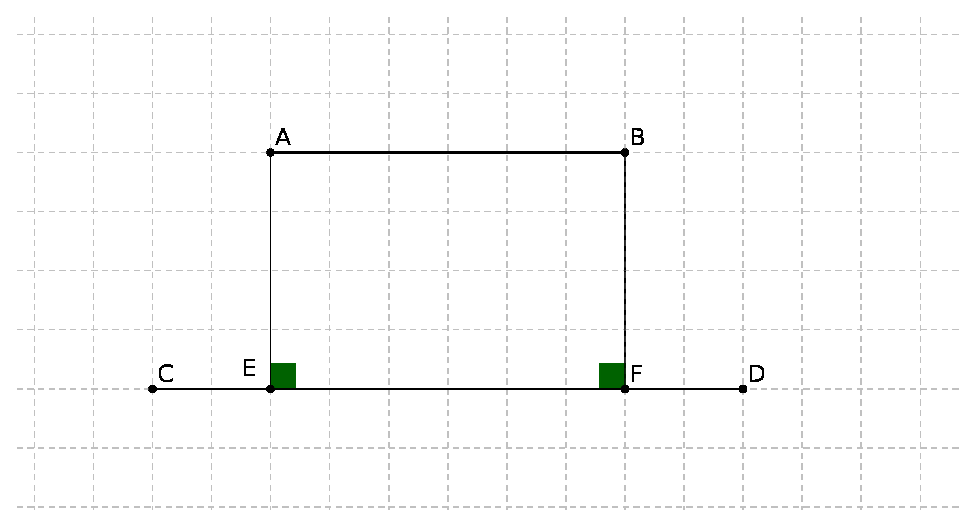
\includegraphics[scale=0.7]{figures/posid.eps}     
  
 On peut démontrer que ABFE est un parallélogramme. Pour démontrer que AE=BF il faut démontrer que dans un parallélogramme les côtés opposés ont même longueur. Or ce théorème se montre à partir du théoème 34 du livre 1 d'Euclide, théorème qui repose ... sur P5. Donc la définition de Posidonius repose sur P5.\\
  
  
   
   
   
   
  
   Ainsi Posidonius ne démontre pas P5.\\
   
   On voit là la difficulté qu'ont eu les mathématiciens (qui étaient pourtant très bons) de sortir de l'"évidence".\
   
   \textit{Remarque:} on voit apparaître ci-dessus qu'un questionnement autour de P5 est lié à un questionnement sur le parallélogramme ou le rectangle. 

  \subsection{Proclus: (410-483 ap.J.C.):}\


Proclus critique Posidonius et propose la démarche suivante: il veut d'abord démontrer que si une droite coupe une autre droite elle coupera aussi toutes les parallèles à cette droite.\


     Pour démontrer cela il considère deux droites parallèles (AB) et (CD) et une droite (BE) tel que E et (CD) sont situés du même  côté  de (AB) et on considère la distance EH de E à (AB). La droite (BE) pouvant se prolonger (postulat 1 d'Euclide) autant qu'on veut la distance EH viendra plus grande que la distance des deux parallèles donc (BE) coupera (CD).

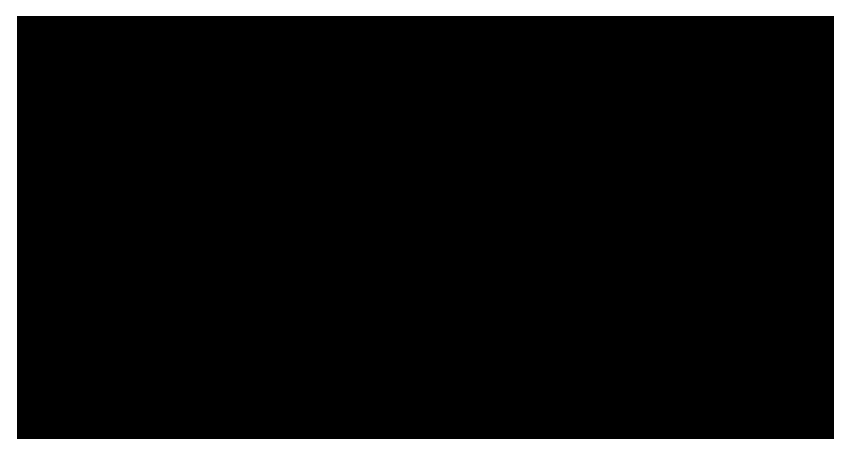
\includegraphics[width=10cm]{figures/proclus.eps} \

   Mais une fois encore, cela revient à considérer que deux droites parallèles sont équidistantes, résultat qui est une conséquence de P5.\\
   

  Avant les mathématiciens arabes  d'autres philosophes se sont intéressés au problème. On peut citer l'astronome Ptolémée (IIIeme siècle) ou Simplicius.  
    
  
  \section{Mathématiciens arabes (1)}
  
   Nous parlerons de Al Jawhari (Xe),Thabit b. Qurra(Xe), Ibn al-Haytam(XIe), Al Khayyam(XIe).\bigskip 
   
   Répétons que lorsque l'on essaie de se remettre dans les mêmes conditions que ceux qui ont essayé de démontrer P5, on s'aperçoit que, assez rapidement, on est amené à se poser les mêmes questions, à tourner autour de la somme des angles d'un triangle, à introduire un quadrilatère dont trois angles sont droits, à étudier le lien entre droites parallèles et équidistance, etc... 
   
   \subsection{Al Jawhari}
   
  Al Jawhari affirme que, par un point quelconque situé à l'intérieur d'un angle, il est possible de tracer une ligne coupant ses deux côtés. \\
  
  
  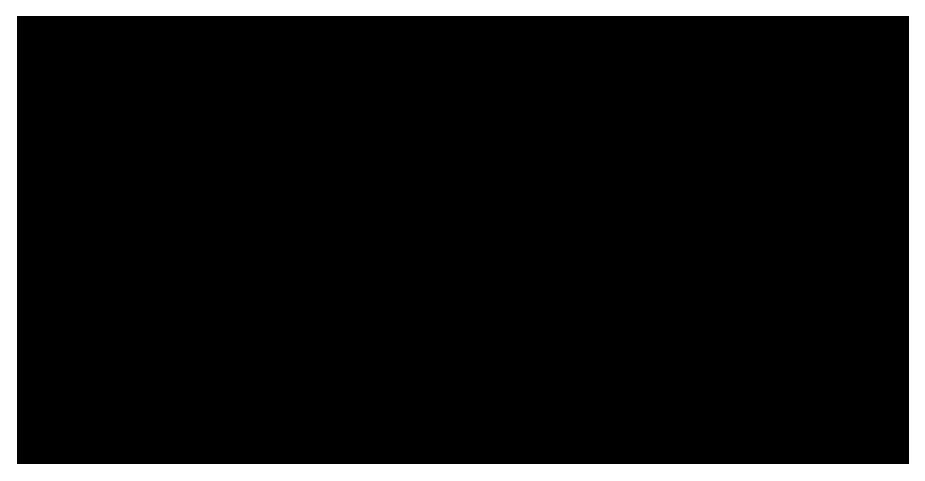
\includegraphics[scale=0.7]{figures/ALJAHW2.eps} 
  
  
 
   
  \footnote{ (1) Pour les mathématiques arabes on peut se réferrer au livre " Histoire des sciences arabes " édité sous la direction de Roshdi Rashed.
   Il est intéressant de se rendre compte de l'influence arabe sur les savoirs. Si l'influence grecque est considérable aux VIe, Ve, IVe siècle avant J.C., après la fin de la puissance politique des cités grecques (victoire d'Alexandre le Grand en -338), les centres culturels se déplacent au moyen orient, en particulier à Alexandrie. Même si la langue grecque est la langue du savoir, les savants à Alexandrie ne sont pas grecs : citons Euclide, Eratostène né dans une petite ville de l'actuelle Lybie et St Augustin le plus grand penseur chrétien du Moyen Age né dans une petite ville de l'actuelle Kabylie. Les Arabes, au VIIe siècle,(qui sont au départ très peu nombreux) vont s'installer aux bords de la méditérannée en y apportant une stabilité politique, une langue et une religion qui  demande aux croyants de développer leur connaissance du monde. } 
   
    Puis il se propose de démontrer P5. Cet énoncé qui a l'air bien loin de P5 en est une conséquence. On peut prouver que les deux énoncés sont équivalents. (cf à la démonstration dans le chapitre suivant). Donc prendre comme postulat l'énoncé de   Al Jawhari revient à prendre P5. \bigskip 
  
  
   
   Donc P5 n'est pas toujours démontré et à quel point il a été, une fois de plus, difficile de s'abstraire de l'évidence. 
   
    \subsection{Thabit b. Qurra}
   
   Thabit b. Qurra propose deux démonstrations:\bigskip 
   
   
    la première repose sur le principe suivant:\textit{ si deux droites coupées par une troisième se rapprochent ou s'éloignent l'une de l'autre quand on les trace dans une direction, elles s'éloignent ou se rapprochent quand on les trace dans l'autre direction.} Mais une fois de plus cet énoncé est équivalent à P5: en effet c'est P5 exprimé autrement!\bigskip 
    
    

   
   

 
   Il est à noter que Lobatchevski dans sa GNE où tous les axiomes euclidiens sont vérifiés sauf P5 il existe des lignes droites qui s'écartent l'une de l'autre dans chacune des directions à partir de leur perpendiculaire commune.\bigskip 
   
     La deuxième démonstration repose sur l'hypothèse suivante: \textit{si on déplace une droite D perpendiculaire à une droite donnée chaque point de D décrira une droite équidistante à la droite donnée.} \bigskip 
      
    
    Cette hypothèse n'est en fait vraie que dans la géométrie euclidienne! 
  b.Qurra déduira de ce principe la construction d'un rectangle qui est celui décrit plus haut puis démontrera P5. Mais de nouveau cet énoncé sera équivalent à P5.
  De plus l'hypothèse dont il part implique la création d'une distance. Ce qui , une fois de plus, est impossible.\bigskip 
 
   
     La démarche de Qurra sera critiquée, en particulier par Al-Khayam.\
     
     
En effet b.Qurra utilise la notion de mouvement: il affirme qu'un point se déplaçant crée une ligne ce qui pour Al-Khayam se référant à Aristote était un non sens.
\bigskip 

 En effet pour ce dernier la connaissance d'un objet géométrique repose sur sa connaissance dans notre espace à trois dimensions. Ainsi  on doit partir du solide sensible puis passer au solide géométrique, abstrait des sensations qui lui sont liés, (premier degré d'abstraction) puis,\
 
  une surface faisant partie d'un solide, si on la sépare du solide on aboutit à un deuxième niveau d'abstraction. Une ligne est sur une surface et si on l'enlève de la surface on a un troisième niveau d'abstraction. \
  
  Quant au point il est sur une ligne et si on le retire de la ligne on passe à un quatrième niveau d'abstraction. 
  \
  
  
 En  résumé, une surface ne peut pas engendrer un solide puisque c'est le solide qui crée la surface, une ligne ne peut pas créer une surface puisque c'est la surface qui crée la ligne, un point ne peut pas engendrer une ligne puisque c'est la ligne qui le crée. Donc l'approche de Qurra sera considérée, par Al Kahiam comme fausse.\\
 
 Pour Aristote  seuls les corps réels du monde sensible sont soumis au mouvement donc les objets géométriques qui sont des abstractions, non. Et Euclide a cherché à éviter le plus possible  les mouvements de figures. Cependant l'axiome 8 qui affirme que deux figures qui s'ajustent sont égales et comment fait-on pour ajuster deux figures sans déplacement? Ce problème divisera les savants pendant de nombreux siècles!
 
 Cette objection de Al Kahiam est intéressante parce qu'elle prouve qu'il y a eu une réflexion sur ce qu'est l'espace géométrique. Cet espace mathématique n'est en aucun cas l'espace physique. Mais cette réflexion ne va pas suffisamment loin, puisque malgré tout cet espace géométrique dérive de l'image que l'on a de l'espace physique. Tant que l'on ne dépassera pas cette conception on sera bloqué.\\
 
  
  \subsection{Ibn al-Haytam:}

   Cette idée de rectangle sera réutilisée par  Ibn al-Haytam: il introduit un quadrilatère qui a trois angles droits. Pour lui le quatrième angle sera soit obtus, soit aigu, soit droit. Il réfute les deux premières possibilités, affirme que l'angle est droit et démontre P5. 
   Mais réfuter les deux premières possibilités revient à admettre P5. Une fois de plus Ibn al-Haytam n'y arrive pas.\
   
    Il est à noter que \textbf{ce rectangle va être utilisé par le mathématicien Lambert au XVIIIe pour tenter de démontrer P5.}

On peut noter que les deux premières possibilités pour le quatrième angle correspondront respectivement aux géométries hyperboliques et elliptiques premières géométries non euclidiennes du XIXe !  

\subsection{Al Khayyam:}


Celui-ci affirme que ses prédécesseurs se sont trompés parce qu'ils n'ont pas tenu compte des principes qu'Aristote auraient énoncés dans un ouvrage qui ne nous est pas parvenu.\

Al Khayyam énonce le quatrième de ces principes qu'il va utiliser: deux lignes droites convergentes se coupent et il est impossible à deux droites convergentes de diverger dans la direction dans laquelle elles convergent.

   Al Khayyam va donc utiliser ce principe. Puis, lui aussi, considère un rectangle dans lequel il y a deux angles droits et deux côtés latéraux égaux et se demande comment sont les deux autres angles. A l'aide de ce principe il démontre que les deux angles qui restent sont droits puis prouve P5. Mais pour démontrer cela non seulement il utilise ce principe  d'Aristote mais aussi un théorème qui...résulte de P5! Donc une fois de plus P5 n'est pas démontré. (cf chapitre suivant pour le détail de la démonstration )
    Mais ce travail n'est pas inutile: \textbf{il sera poursuivi par le jésuite Saccheri au XVIIIe }.
 
   D'autres mathématiciens arabes travailleront sur le sujet mais tous ont en tête une seule géométrie possible: l'euclidienne. Aucun ne franchira le pas fait au XIXe et pourtant ce sont tous des esprits puissants, des chercheurs qui ont la force de sortir de leurs certitudes.\bigskip 
   
    Et pour y arriver il faudra remettre en cause les évidences du type: deux droites parallèles sont équidistantes, dans un quadrilatère qui possède déjà trois angles droits le quatrième l'est aussi, par un point pris dans un triangle on peut tracer une droite coupant deux côtés du triangle, etc...\\
    
    En fait, pour sortir de la géométrie euclidienne, il faut admettre que  l'univers, dans lequel on vit, peut être décrit  avec d'autres modèles que ceux que nous connaissons. Si on considère que nous avons une connaissance totale de l'univers toute autre approche devra être fausse. C'est pour cela que l'on va essayer de démontrer pendant des siècles et des siècles qu'il n'y a qu'une seule géométrie de vraie et que ne pas y arriver est un échec important.\\
    
    Il faut cependant souligner que ces tentatives de démonstration de P5, même si elles sont des échecs, préparent les travaux de Gauss, Bolyai ou Lobatchevski. Il s'agit d'un long cheminement et ces recherchent permettent de mettre en évidence des manques, des insuffisances (par exemple: problème de la mesure d'une longueur) et de poser de nouvelles questions. 
    
    
 \section{Tentatives de démonstrations à partir du XVIIe:}
 
 Nous parlerons de Wallis(1616-1703), Saccheri(1667-1733), Lambert(1728-1777)  et Legendre (1762-1833).
     
     
     \subsection{Wallis : mathématicien écossais.}
     
     Wallis, en plus de ses activités mathématiques (ceux qui ont fait un peu de maths ont entendu l'expression "intégrales de Wallis),  est l'auteur du premier traité de phonétique de la langue anglaise, en introduction à sa \textit{Grammatica Linguae Anglicanae}. Il est également connu comme précurseur de l’éducation des sourds-muets.\\
     
   Le postulat 3 d'Euclide demande à ce que l'on puisse construire un cercle. On peut remarquer que tous les cercles sont semblables, c'est à dire que l'on passe de l'un à l'autre par un déplacement ou un agrandissement ou une réduction, Wallis va avoir l'idée de remplacer P5 par le postulat: \textit{sur une droite donnée il est possible de construire un triangle semblable à un triangle donné(c'est à dire un triangle qui aura les mêmes angles que le triangle donné).} On passera d'un triangle semblable à un autre, comme pour les cercles, par un agrandissement ou une réduction.

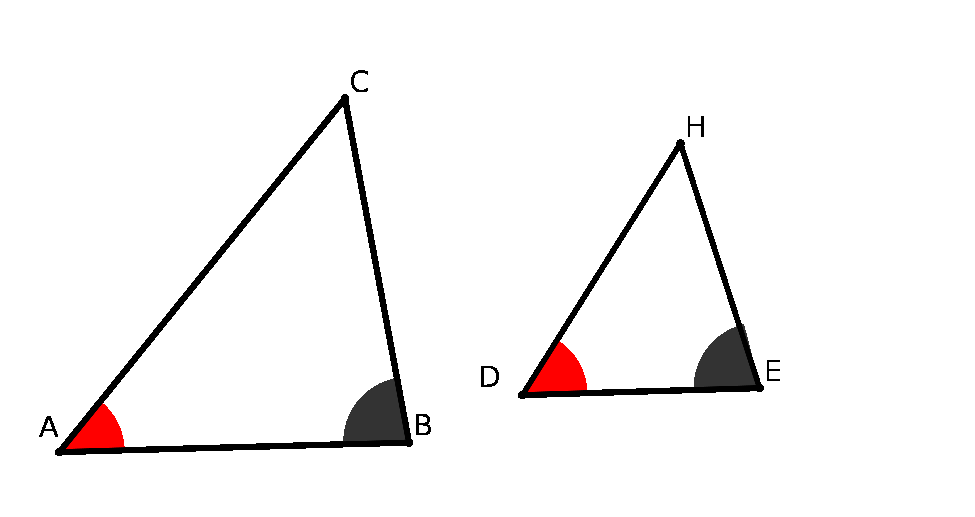
\includegraphics[scale=0.8]{figures/WAL1.eps} 


   Ceci semble tellement évident que personne ne se rendit compte que le postulat de Wallis se déduit de P5.

En effet cela revient à supposer que la somme des angles dans un triangle est égale à deux droits donc à supposer P5 vrai! donc on n'avance pas! Plus précisément la similitude des triangles est traitée dans le livre 6 d'Euclide. L'existence des triangles semblables repose sur des théorèmes qui utilisent P5. \bigskip 

 Il est cependant étonnant que Wallis, qui était un très bon mathématicien et qui connaissait sans doute très bien les Eléments d'Euclide ne s'en soit pas rendu compte... sauf si, comme beaucoup d'autres,\textbf{ il pensait que l'évidence était une vérité.} 

 \subsection{Girolamo Saccheri: (1)}

Saccheri  utilise le même quadrilatère que   Al Khayyam: il prend donc un quadrilatère ABDC dans lequel les angles A et B sont droits et les côtés AC et BD sont égaux.

  
 \footnote{(1) Saccheri est un jésuite professeur de philosophie, théologie et mathématique qui a publié en 1733 un ouvrage tombé dans l'oubli et retrouvé au XIXe par Beltrami. Ce dernier pensait que Sacchéri était le premier à avoir créé une géométrie non euclidienne.}
 
  
 
 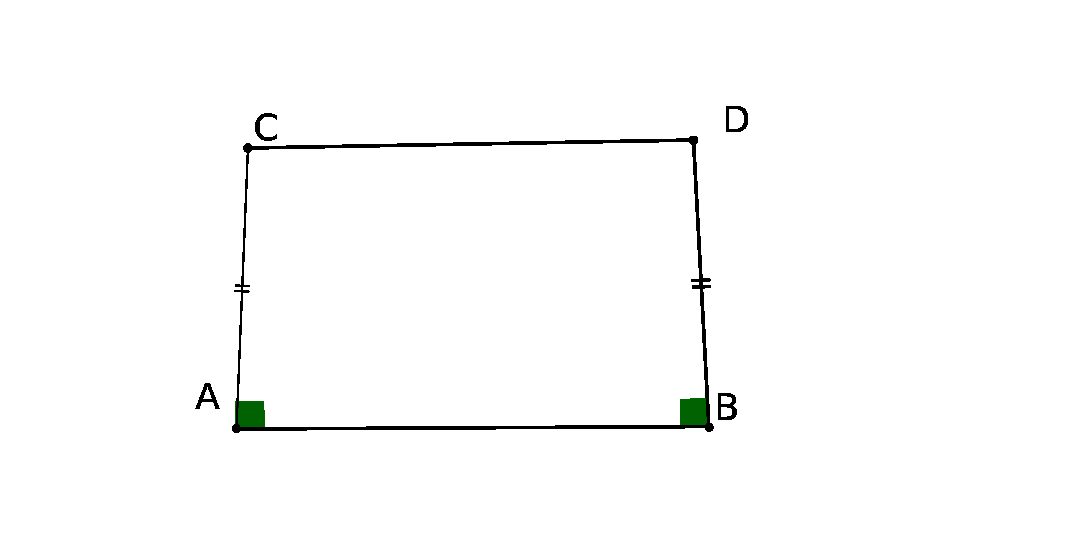
\includegraphics[width=11cm]{figures/sac.eps}  \bigskip 
 
  Naturellement, pour quelqu'un qui n'a en tête que la géométrie euclidienne ce quadrilatère est un rectangle... 
 


 
   

 
 Saccheri fait alors les trois hypothèses suivantes: \\
H1: les angles C et D sont droits,\\
H2: ils sont obtus,\\
H3: ils sont aigus.\bigskip



  
     Il démontre alors que si l'une des trois hypothèses est vraie dans un quadrilatère alors elle est vraie dans tous les autres quadrilatères puis il démontre que la somme des angles dans un triangle est
       \\
       sous H1, égale à deux angles droits,\\
      sous H2, supérieure à deux angles droits,\\
      sous H3, inférieure à deux angles droits.\\ 
      
 Pour démontrer P5, il considère la figure suivante, dans laquelle AP et PB sont perpendiculaires et l'angle fait par AP et AD est aigu.
  

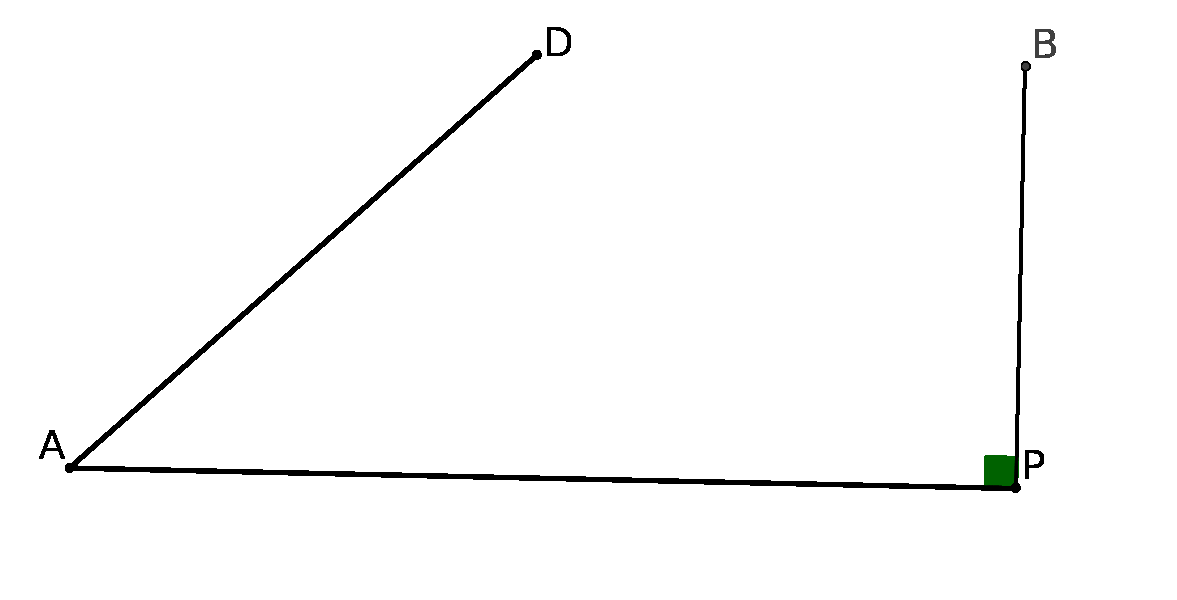
\includegraphics[scale=0.5]{figures/sacc2002.eps} 
   
  Il se place dans chacune des hypothèses H1, H2 et H3 et essaie de démontrer P5.\\
  

Sous H1 (les angles C et D sont droits) il démontre que AD coupera PB donc P5.(Voir dans le chapitre suivant une démonstration).\\


Sous H2 (les angles C et D sont obtus) il démontre aussi que AD coupera BP et donc P5 et comme P5 implique que la somme des angles dans un triangle est égale à 180 degrés il tombe sur une contradiction et donc rejette H2. Mais... cela prouve simplement que dans sa démonstration il y a un problème  et on verra pourquoi dans le chapitre suivant.\\



Sous H3 (les angles C et D sont aigus) il n'arrive pas à une contradiction et démontre même des propriétés telles que:\

  Deux droites sont:
soit sécantes,
soit admettent une perpendiculaire commune et alors elles "divergent",
soit  elles sont "asymptotes" l'une de l'autre.\


N'arrivant pas à une contradiction, il abandonne et trouve ses résultats insupportables!\bigskip 


En fait Saccheri peut être considéré comme celui qui a établi les premiers résultats de géométrie non euclidienne mais les trouvant horribles et opposés au bon sens il ne les publiera pas. Il sera redécouvert par le mathématicien italien Beltrami au XIXe siècle.

\newpage \subsection{Johann Heinrich Lambert:(1)}


   Lambert connaît les travaux de Saccheri, mais préfère s’appuyer, comme Ibn al-Haytam, sur un quadrilatère à trois angles droits. Il fait alors trois hypothèses:
              le quatrième angle est, soit droit, soit aigu, soit obtus.\\
              
  *Sous l'hypothèse de l'angle droit il démontre P5.
  
  **Il rejette l'hypothèse de l'angle obtus en faisant la même erreur que Saccheri.

  *** Sous l'hypothèse de l'angle aigu, il obtient un certains nombre de résultats et n'arrive pas à une contradiction!\bigskip 
  
  
    Mais il démontre des résultats de la géométrie  non euclidienne tels que la somme des angles d'un triangle est inférieure à 180 degrés ou encore l'ensemble des points situés   à égale distance  d'une droite donnée n'est pas une droite! Ou encore qu'il n'y a pas, sous cette hypothèse, de triangles semblables... (cf chapitre 2 pour quelques démonstrations). De plus il est le premier à démontrer que la somme des angles d'un triangle dépend de son aire.\bigskip 
   
   
    
    Mais comme Saccheri, Lambert renonce à aller plus loin: il est en effet, comme tout le monde à l’époque, de philosophie Kantienne : les axiomes de la géométrie doivent être le reflet des propriétés de l’espace sensible. 
    
    
  \footnote{(1) Johann Heinrich Lambert (1728-1777) est un mathématicien (philosophe et physicien) né à Mulhouse (ville libre, république depuis 1347, exclave des cantons suisses donc ni française, ni allemande mais rattachée à la France en 1798).
   Il fait une grande partie de sa carrière à Berlin et, en autres choses, a démontré que le nombre Pi était irrationnel. } 
  

\newpage \subsection{Adrien Marie LEGENDRE: (1752-1833) (1)}

Il est le dernier mathématicien avant les créateurs des GNE à s'être intéressé au problème des parallèles.\\
 
   Pour démontrer P5 il démontre en particulier que la somme des angles d'un triangle est égale à 180 degrés et cela de manière tout à fait intéressante:\\
   
   
   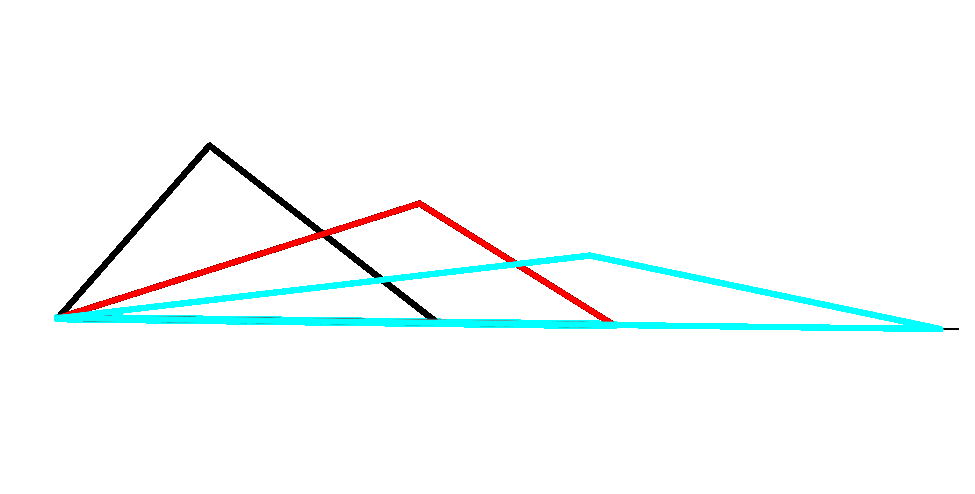
\includegraphics[scale=1]{figures/Leg1.eps} 
   
   
    il construit une succession de triangles (sur la figure, noir, rouge, bleu) dont les angles à la base tendent vers 0 mais dont la somme des angles ne varie pas. Il pense alors démontrer que le troisième angle du triangle tend vers 180 degrés mais c'est là où il se trompe. (cf chapitre 2 pour la démonstration)\bigskip
 
   
   
   
   
    Son passage à la limite  revient à supposer que P5 est vrai! Donc une fois de plus on tourne en rond. (cf chapitre suivant pour la démonstration)\bigskip 
   \bigskip
   \bigskip
   \bigskip 
 \footnote{(1) Legendre a démontré un certain nombre de choses intéressantes mais ses travaux ont surtout servi de base de travail aux mathématiciens tels que Gauss, Abel ou Galois. Soucieux de simplifier les Eléments d'Euclide Legendre écrivit l'un des plus grands succès de l'édition scolaire:  Éléments de géométrie qui fut traduit en anglais et en allemand et qui fit référence pendant au moins cinquante ans.}   


\chapter{Positions philosophiques aux XVII-XVIIIe siècles:}

\section{Newton:
    }
 L’espace aristotélicien, donc des grecs, est essentiellement qualitatif et parfaitement hiérarchisé. Il est fondé sur l'expérience et nos sens. Pour Aristote, les mathématiques ne peuvent pas  expliquer le monde réel.\
 
 Cette conception présente cependant présente un avantage: elle permet de ne pas lier la géométrie au cosmos et donc de pouvoir envisager comme hypothèse "la somme des angles dans un triangle n'est pas égale à 180 degrés" comme possible, même si cette hypothèse n'a pas été exploitée.\\
 
 
    C'est Galilée qui va détruire le cosmos grec et c'est en cela qu'il est révolutionnaire. Il faut reconnaître qu'il était de plus en plus difficile d'expliquer les phénomènes astronomiques par la physique d'Aristote: la connaissance du mouvement des planètes ou des astres devient de plus en plus précis et nécessite des calculs de plus en plus compliqués si l'on veut rester dans un système géocentrique (cf à la théorie des épicycles).\
    
     Galilée va géométriser l'univers, son espace est mathématique.\\
    
    C'est dans cet espace neutre, absolu, indépendant des objets qui s'y trouvent que Newton va formuler ses lois. Cet espace est euclidien. Ainsi, non seulement la géométrie restera l'art du raisonnement pur mais en plus la Nature devra s'y soumettre. Ce n'est pas un hasard si Newton parle de Principes mathématiques de la Philosophie Naturelle. \\
    Le génie de Newton ne peut que conforter ceux qui veulent démontrer P5 et refuser toute autre hypothèse. \\
  
  \section{Pascal}
      
    
  Dans le texte \textit{"
  De l'esprit géométrique et de l'art de persuader"} Pascal exprime parfaitement son point de vue.\
  
 Tout d'abord la "\textit{véritable méthode, qui formerait les démonstrations dans la plus haute excellence, s'il était possible d'y arriver, consisterait en deux choses principales: l'une de n'employer aucun terme dont on n'eût auparavant expliqué nettement le sens, l'autre, de n'avancer jamais aucune proposition qu'on ne démontrât par des vérités déjà connues.}"\
 
 Donc il faudrait tout définir et tout démontrer, ce qui, pour Pascal, est impossible. En effet "\textit{il est évident que les premiers termes que l'on voudrait définir, en supposeraient de précédents pour servir à leur explication...et en poussant les recherches de plus en plus, on arrive nécessairement à des mots primitifs qu'on ne peut plus définir}". Donc construire une science parfaite est impossible pour l'être humain. Mais, pour Pascal, il ne faut pas renoncer à la science. C'est la géométrie qui est la plus proche, bien qu'imparfaite, des  exigences dans la recherche de la perfection.\\
 
 Citons encore Pascal: "\textit{On trouvera peut-être étrange que la géométrie ne puisse définir aucune des choses qu'elle a pour principaux objets: car elle ne peut définir ni le mouvement, ni les nombres, ni l'espace...mais on ne sera pas surpris, si l'on remarque que cette admirable science ne s'attachant qu'aux choses les plus simples, cette même qualité qui les rend dignes d'être ses objets, les rend incapables d'être définies; de telle sorte que le manque de définition est plutôt une perfection qu'un défaut, parce qu'il ne vient pas de leur obscurité, mais au contraire de leur extrême évidence}".\
 
 Ainsi on n'a pas à définir ni les nombres, ni l'espace. Or ce sont justement les travaux sur les nombres et l'espace qui vont permettre la création des géométries non euclidiennes. Pascal ferme ainsi l'ouverture sur toute géométrie autre que celle d'Euclide.\\

\section{Descartes}
  
 

 
 Citons Descartes à partir de son "\textit{Discours de la méthode}". Son premier précepte est "\textit{de ne recevoir jamais aucune chose pour vraie, que je ne la connusse évidemment être telle : c'est-à-dire, d'éviter soigneusement la précipitation et la prévention; et de ne comprendre rien de plus en mes jugements, que ce qui se présenterait si clairement et si distinctement à mon esprit, que je n'eusse aucune occasion de le mettre en doute.}" 
 
Mais comment juger d'une évidence? Descartes nous dit:\


"\textit{Et remarquant que cette vérité: je pense, donc je suis, était si ferme et si assurée, que toutes les plus extravagantes suppositions des sceptiques n'étaient pas capables de l'ébranler, je jugeai que je pouvais la recevoir, sans scrupule, pour le premier principe de la philosophie que je cherchais.}"\

Plus loin il rajoute:\

 
 
" \textit{je jugeai que je pouvais prendre pour règle générale, que les choses que nous concevons fort clairement et fort distinctement sont toutes vraies; mais qu'il y a seulement quelque difficulté à bien remarquer quelles sont celles que nous concevons distinctement. En suite de quoi, faisant réflexion sur ce que je doutais, et que, par conséquent, mon être n'était pas tout parfait, car je voyais clairement que c'était une plus grande perfection de connaître que de douter, je m'avisai de chercher d'où j'avais appris à penser à quelque chose de plus parfait que je n'étais; et je connus évidemment que ce devait être de quelque nature qui fût en effet plus parfaite. Pour ce qui est des pensées que j'avais de plusieurs autres choses hors de moi, comme du ciel, de la terre, de la lumière, de la chaleur, et de mille autres, je n'étais point tant en peine de savoir d'où elles venaient, à cause que, ne remarquant rien en elles qui me semblât les rendre supérieures à moi, je pouvais croire que, si elles étaient vraies, c'étaient des dépendances de ma nature, en tant qu'elle avait quelque perfection; et si elles ne l'étaient pas, que je les tenais du néant, c'est-à-dire qu'elles étaient en moi, parce que j'avais du défaut. Mais ce ne pouvait être le même de l'idée d'un être plus parfait que le mien : car, de la tenir du néant, c'était chose manifestement impossible; et parce qu'il n'y a pas moins de répugnance que le plus parfait soit une suite et une dépendance du moins parfait, qu'il y en a que de rien procède quelque chose, je 
ne la pouvais tenir non plus de moi-même. De façon qu'il restait qu'elle eût été mise en moi par une nature qui fût véritablement plus parfaite que je n'étais, et même qui eût en soi toutes les perfections dont je pouvais avoir quelque idée, c'est-à-dire, pour m'expliquer en un mot, qui fût Dieu. }"\


Ainsi, pour Descartes, "je pense donc je suis" est  la preuve de son existence, donc des choses qu'il conçoit clairement et distinctement, évidences qui lui viennent de Dieu.\

 Cet espace physique dans lequel nous vivons étant une évidence, on ne peut pas le remettre en cause. Cet espace pour Descartes est euclidien et si la géométrie n'a d'autre utilité que servir ou illustrer cet espace, il n'y a pas de place pour une autre géométrie. Ainsi le postulat cinq doit être démontrable ou alors sa négation doit conduire à une contradiction. Saccheri, en particulier n'y arrive pas. D'où son dépit.

   
   \section{Kant:}
   
    Avant Kant, il y avait un espace dans lequel un certain
nombre d’objets de toutes natures se déplaçaient et nous, êtres humains, nous
observions ces objets grâce à nos cinq sens. Cet espace est réel. 

 Kant ne se prononce pas sur sa réalité. L’espace est une donnée à priori indépendante de toute expérience. Il est à la base de toutes nos intuitions concernant ce qui nous entoure. Cet espace ne peut se représenter que d'une seule manière: il est euclidien à trois dimensions.\
   
    De plus, pour Kant, comme pour les  autres philosophes ou mathématiciens de cette époque, la géométrie euclidienne est le prototype de la pensée claire et du raisonnement logique. Emmanuel Kant pensait que ce prototype  était inscrit dans le cerveau humain. C'est lui qui nous permet de percevoir le monde extérieur.\\
    
   
  
  
   
  Donc toute géométrie non euclidienne serait un non sens.\\






 


\section{Conclusion:}

Le XVIIeme et le XVIIIeme siècles sont donc très peu favorables à la découverte ou à la création d'autres géométries.\

  La remise en cause de ces conceptions se fera par la reconstruction des mathématiques, par la redéfinition de leur place dans l'ensemble des connaissances, par celle de la géométrie dans les mathématiques, par la remise en cause de l'espace physique newtonien avec, par exemple, Maxwell et, surtout, Einstein.\
 
Toutes ces questions seront débattues au XIXeme et au XXeme siècle .\\

 

   \chapter{Géométrie non euclidiennes avec Lobatchevski et Bolyai:}
   \section{ Naissance difficile:}
     Il y a une permanence dans l’histoire des mathématiques: quand un nouveau concept apparaît il est d’abord rejeté car trop "abstrait". Puis accepté avec réticence car il est utile dans les applications. Enfin il est pleinement reçu quand il est reconstruit de manière à être cohérent avec le reste des connaissances mathématiques.\\
     
     

  Deux exemples:
  D’abord les nombres négatifs qui sont considérés comme des nombres "faux" (Descartes). Dans l’Encyclopédie de Diderot-d’Alembert, on voit bien qu’ils n’ont pas toujours de statut: en effet les nombres sont liés indissolublement aux grandeurs géométriques et une grandeur géométrique est un nombre positif. En fait c’est la notion de nombre qui ne sera clairement défini qu'à la fin du XIXe siècle!\\
  

   Ensuite le "nombre imaginaire ou complexe" $i$ dont le carré est égal à -1, est introduit au XVIème . Ce nombre dont le carré est négatif est en contradiction complète avec les connaissances de l’époque. Il va pourtant être utilisé car il permet de résoudre de nouvelles équations. Les nombres dits "complexes" ne seront construits correctement qu'à la fin du XIXe.\\
   

   Quant aux géométries non euclidiennes elles mettront 21 siècles à exister malgré la
démarche d’Euclide qui incite à les construire! Il faut bien dire "à exister", parce  qu'elles ont déjà été en partie élaborées (Saccheri, certains mathématiciens arabes) mais  c'est leur existence que l'on a refusé d'admettre!  Pourquoi un accouchement si difficile?\\


  Il y a plusieurs raisons (dont il est difficile de faire la liste!).\\
  
–- A quoi bon créer une géométrie qui ne serait pas supérieure à la première, qui n’aurait aucune application ni en mathématique, ni dans le monde sensible? La curiosité a beau être un moteur dans la recherche mathématique elle a aussi ses limites!\\

–-l’Univers est géré depuis Galilée, Newton et Descartes par la géométrie euclidienne. Il  faut réaliser que certains universitaires, à la fin du XIXe, ne prennent plus d'étudiants chercheurs en physique parce qu'il n'y aurait plus rien à découvrir!\\

–- Il y a la position philosophique de Kant.\\

–-  Peut être que l'on ne peut pas imaginer qu'il y a plusieurs géométries vraies. Comment serait-il possible qu'en niant (au sens 
logique) la géométrie euclidienne on obtienne une autre théorie tout aussi vraie? Et la question que l'on doit se poser est le sens que l'on donne à vrai.\\

--- Enfin la raison la plus forte est, sans doute à chercher dans les mathématiques elles mêmes: quelle est leur place? qu'y fait-on exactement? Qu'est-ce qu'une activité mathématique?\\

\section{Premières géométries non euclidiennes: }

Comment peut-on expliquer qu'au début du XIXe trois mathématiciens vont élaborer presque simultanément (entre 1820 et 1840), (mais sans être au courant du travail des autres), une géométrie non euclidienne?
 On pourrait donner plusieurs raisons:\
 
 
 
  La première c'est peut-être la Révolution Française: en effet elle va inciter les hommes à revendiquer leur liberté et donc la liberté de créer indépendamment  de l'académisme (voire contre). Indépendamment de la Révolution Française, créer une nouvelle théorie dans quelque domaine que ce soit est une revendication de liberté!\
  
  
 La deuxième, et c'est sans doute la plus importante, c'est l'explosion des mathématiques avec Pascal, Descartes, Euler, Lagrange et bien d'autres, les Eléments d'Euclide ne pouvant plus être leur synthèse.\
 
 La troisième est le travail accumulé au cours des siècles passés sur le sujet.\\
 
 

 Les trois précurseurs principaux sont Gauss, Bolyai et Lobatchevski:

  Ce qui distingue fondamentalement ces mathématiciens de ceux qui les ont précédés c’est leur démarche: ils ont construit une nouvelle géométrie alors que les autres ont essayé de démontrer le postulat des parallèles et que jamais ils n’ont mis en doute l’idée qu’il y avait une seule géométrie.
  
  Mais ils ont eu très peu de succès:
 
 Lobatchevski a publié ses travaux en russe et a été peu lu. Il appelait lui-même sa géométrie "imaginaire".
 
  Gauss n’a rien publié par peur de créer trop de scandale ( Il était impensable de créer une nouvelle géométrie...). Peut-être aussi attendait-il que l'expérience physique lui donne raison. Mais comment est validée une théorie mathématique? Jusqu’au début du XIXème par l’évidence et plus particulièrement par l’intuition de l’espace à trois dimensions. C’est cette notion de validation d’une théorie mathématique qui va être discutée et rediscutée au XIXème et au XXème .

  Quant à Bolyai il a été découragé par Gauss qui, affirmait-il, avait déjà tout écrit sur le sujet et par son père lui-même.
\subsection{Intéressons nous à la géométrie de Lobatchevski:(1)}
  


 On appelle géométrie neutre ( G.N.) l’ensemble des définitions de la géométrie euclidienne, ses  postulats sauf P5, ses axiomes et les théorèmes ne nécessitant pas le postulat des parallèles., c'est à dire les 28 premiers théorèmes.\\
 
 
  Rajoutons à cette géométrie une négation possible du postulat des parallèles. On obtient:\\
  
  P'5: il existe au moins une droite (AB) et au moins un point P n’appartenant pas à (AB) tels qu’il existe au moins deux droites  passant par P et parallèles à (AB).\\
  
 A partir de là on démontre le premier théorème: quel que soit le point P du plan et quelle que soit la droite (AB) ne passant par P, il existe au moins deux droites parallèles à (AB) et passant par P. \\
 
 Puis on démontre un théorème dans lequel on précise, sous les hypothèses précédentes, parmi les droites passant par P, celles qui sont parallèles à (AB) et celles qui ne le sont pas.\\
 
   On peut alors démontrer que la somme des angles est inférieure à 180 degrés.(Cf au chapitre suivant pour certaines démonstrations).

  Et Lobatchevski va construire une géométrie qu'il va appeler lui-même imaginaire mais totalement cohérente, construction qu'aurait pu faire Saccheri.

   Voici un autre théorème de cette " nouvelle " géométrie : 
  "Si on prolonge de plus en plus loin deux lignes parallèles dans le sens de leur parallélisme, elles s'approcheront de plus en plus l'une de l'autre " .
   

     Et la construction d'une nouvelle géométrie est lancée!\\
     
      \footnote{(1)  Lobatcheski Enfant prodige, à l'âge de 14 ans, Lobatchevski est admis à la toute "jeune" université de Kazan. Il y fera toute sa carrière et en deviendra le recteur : il n'a a alors que 27 ans. 
Assistant dès l'âge de 18 ans, professeur titulaire de mathématiques et d'astronomie à 23 ans, il crée et dirige l'observatoire astronomique. Dès 1826, il publie, en français, son Exposition succincte des principes de la géométrie, une géométrie non euclidienne que Gauss et Bolyai avaient également similairement entrevue mais non publiée. 
Lobatchevski complète ses recherches entre 1830 et 1840 : Sur les fondements de la géométrie, Géométrie imaginaire (1837), Nouveaux fondements de géométrie. (1838), Recherches géométriques sur la théorie des parallèles. (1840, publié à Berlin). }
     
      Poincaré illustrera cette nouvelle géométrie de la manière suivante en inventant un univers dont on donnera  une construction mathématique dans le chapitre 3.\\
  
       On considère un monde dont les habitants sont enfermés dans un demi-plan P  de bord D. Dans cet univers plus un habitant se rapproche du bord de P et plus il devient petit et donc que ses pas tendront vers 0 sans qu'il s'en aperçoive (en effet tout rapetisse autour de lui, ses instruments de mesure compris!).\\
       
  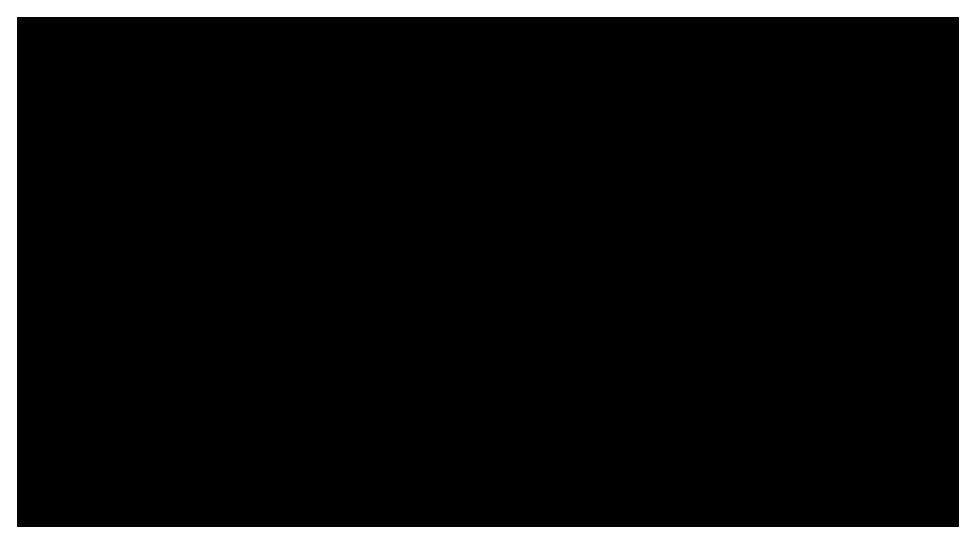
\includegraphics[scale=0.7]{figures/poinc.eps}   
     
        Ainsi il ne pourra jamais atteindre le bord. Nous, de l'extérieur, avec notre œil "euclidien", nous voyons bien que son univers est fini, mais lui le verra infini.\\
     
      Pour joindre un point à un autre cet habitant n'aura pas  toujours intérêt à aller en ligne droite: en effet plus il s'approche du bord et plus ses pas sont petits. Son expérience lui prouve que, pour aller d'un point à un autre, il aura intérêt à procéder de la manière suivante:\\
    
 
 



     
     si les deux points forment une ligne perpendiculaire au bord de P il ira en ligne droite mais si les deux points ne forment pas une ligne perpendiculaire, il parcourra l'arc de cercle joignant les deux points et de centre un point du bord.\\


     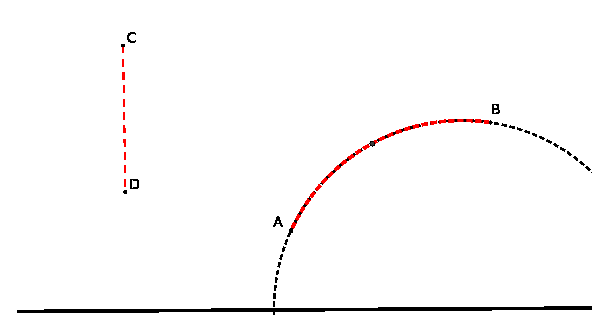
\includegraphics[scale=1]{figures/poinc1.eps}   \\
     
    
     Une droite dans la géométrie euclidienne est le chemin le plus court d'un point à un autre. Si on part de cette définition, dans le demi-plan P les droites seront soit les segments de droites perpendiculaires au bord soit les arcs de cercles  dont le centre est sur le bord. Ces droites vérifient les quatre premiers postulats mais pas P5. 

 
    En effet:
     
    le postulat 1 demande que l'on puisse joindre un point à un autre: dans notre demi-plan on sait joindre un point à un autre parce que l'on sait construire un segment ou un arc de cercle joignant deux points.\\
    
   Le postulat 2 demande que l'on puisse prolonger une droite de chaque côté de manière continue: ici c'est encore vrai:  si on prend un segment de droite perpendiculaire au bord on pourra le prolonger autant qu'on veut puisque plus on sera proche du bord et plus nos pas sont petits donc on se rapprochera du bord indédifiment sans jamais l'atteindre. Pour un arc de cercle c'est encore vrai. \\
    
   Le postulat 3  demande à ce que, à partir d'un point qu'on appelle centre et d'un segment donné on puisse tracer un cercle. Dans notre demi-plan on peut le faire sachant que le cercle obtenu sera comme notre cercle euclidien mais avec un centre décalé.\\
   
Le postulat 4 demande à ce que tous les angles droits soient égaux. Une fois de plus cela sera encore vrai ici ( cela sera détaillé ans le chapitre 3)\\


Le postulat 5 équivaut à l'affirmation suivante: il existe une droite parallèle et une seule à une droite donnée et passant par un point donné. Dans notre demi- plan c'est faux! 

On a tracé, ci-dessous, la figure  sur laquelle on a pris un point C et la "droite" D tracée en bleu. On a tracé aussi les droites "noires" et deux droites "rouge".\\


 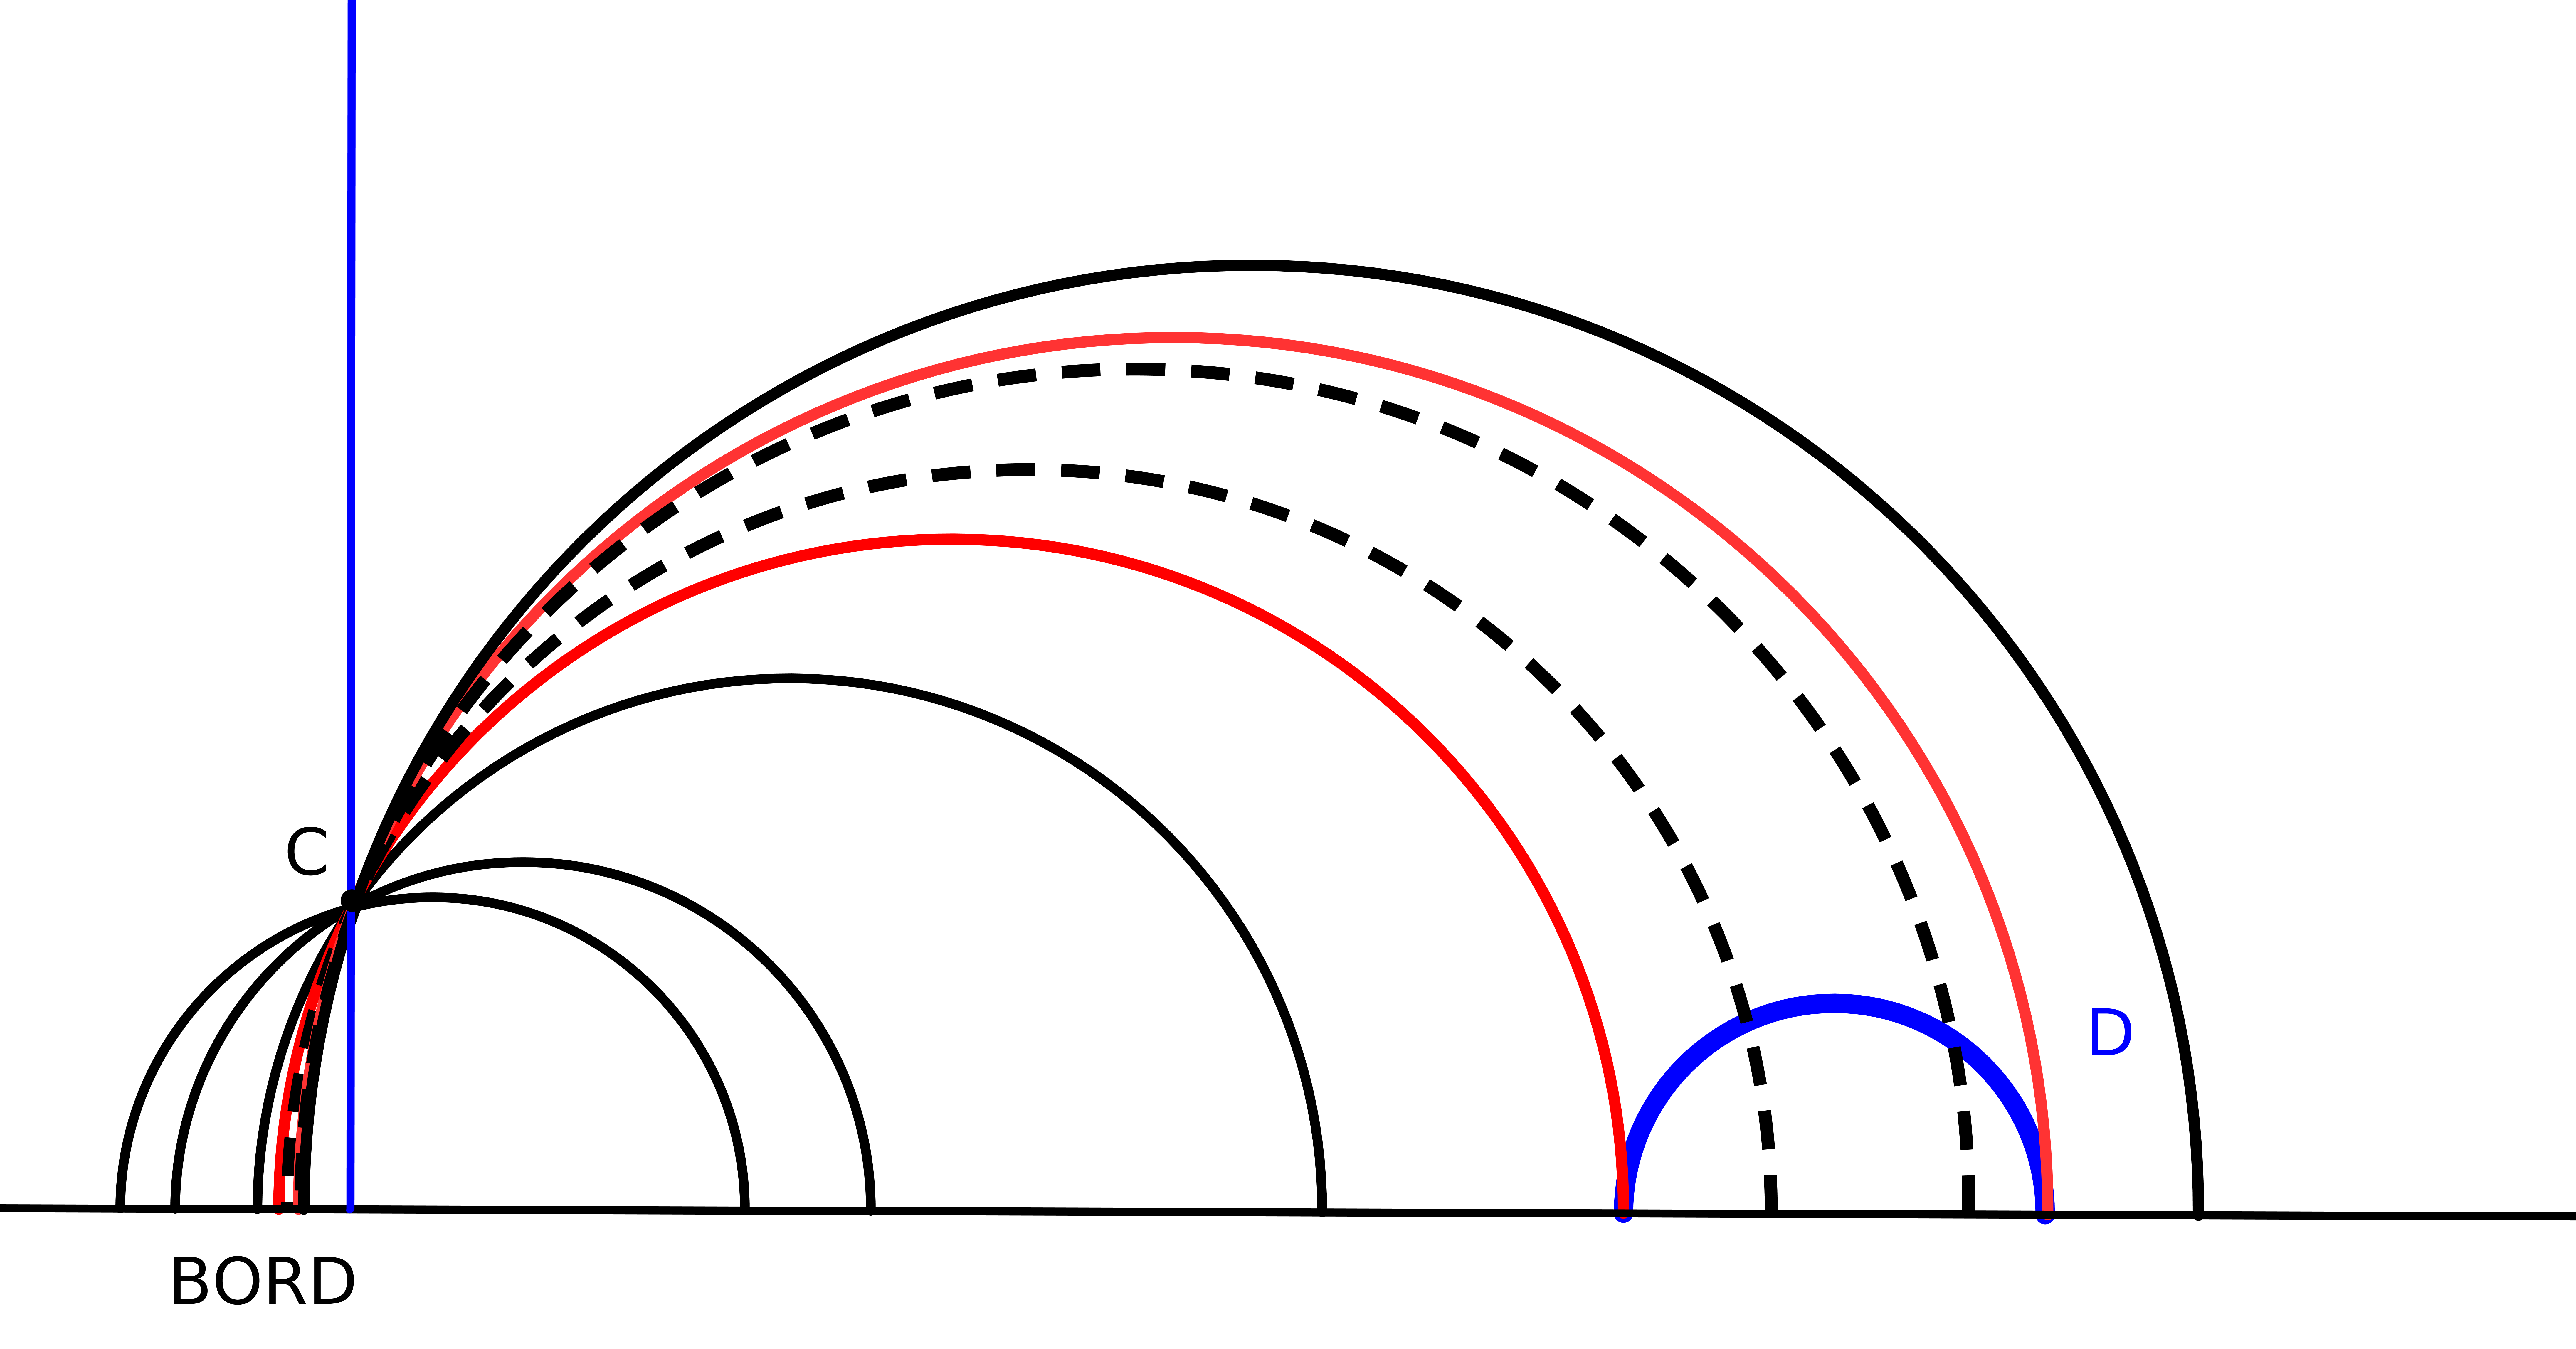
\includegraphics[scale=0.2]{figures/lobat50.eps} \\
 
 
 Il faut insister sur le fait que toutes ces droites se rapprochent indéfiniment  du bord sans le toucher. \\

 
 
    On voit, sur la figure ci-dessus, qu'il existe une infinité de droites parallèles à (D) passant par C . \\
    Les droites situées entre les droites rouges sont sécantes avec D et celles situées en dehors de cette bande passent par C et sont parallèles à D. Il y a donc un infinité de droites passant par un point donné et parallèles à une droite donnée.
    
  \newpage Voilà ce qu'en dit le mathématicien Etienne Gys (contemporain):
" \textit{les  gens (qui vivent dans ce monde) sont raisonnables, ils ne savent pas qu’ils rapetissent. Mais ils sont tout aussi raisonnables que nous qui ignorons probablement beaucoup d’autres choses. La morale de cette petite histoire de Poincaré est qu’on peut très bien envisager beaucoup de mondes extrêmement raisonnables, chacun ayant sa géométrie, chacun ayant sa logique et qui chacun peuvent nous apporter une vision de notre monde concret [...].}"\\


Le mathématicien d'aujourd’hui pour résoudre un problème, pour étudier une question, va utiliser une géométrie, va prendre sa boite à outils, et va choisir la géométrie la plus convenable pour comprendre le problème étudié.\\

Pour conclure voici une phrase de Poincaré:"\textit{Une géométrie ne peut être plus vraie qu’une autre, elle peut simplement être plus commode.}" \\
  
  \subsection{Autres géométries possibles:}
  
     Riemann (1826-1866) va construire une nouvelle géométrie non euclidienne mais par des chemins complètement différents. Il va étudier les propriétés géométriques des surfaces non pas en les replongeant dans l’espace mais en construisant une géométrie sur la surface elle-même.\medskip 
     
 Pour donner un exemple on étudiera les propriétés géométriques d’une sphère indépendamment de l’ espace dans lequel elle appartient: sur la Terre il n’existe pas de droites parallèles...\medskip
 
 Riemann va surtout introduire une nouvelle conception de la distance.
  Nous n’avons absolument pas parler de distance pour l’instant et pourtant c’est une notion qui intervient sans cesse! Qu’est-ce qu’un espace dans lequel il y a une distance?     
 Dans l’espace euclidien, celui de Descartes ou de Newton, les dimensions d’un objet sont les mêmes quelles que soient son lieu, sa vitesse ou son mouvement. \medskip
 Pour Euclide comme pour Newton, la notion de distance comme celle de temps est absolue, universelle. Le rôle de cet espace euclidien se limite à celui d’une étendue indéfinie et neutre, à un réceptacle dans lequel sont plongés les corps.\medskip
 

  Riemann sera le premier à remettre en cause cette conception même si, à son époque, elle est validée par l’ expérience et la physique de Newton. L’espace de Riemann qui est en interaction avec le corps qui s’y déplace, cet espace créé, comme les géométries non euclidiennes, indépendamment de l’ expérience sera validé par...l’expérience, celle de la relativité générale d’Einstein, cinquante ans plus tard. L’espace de cette théorie étant un espace à quatre dimensions, régi par une métrique dépendant de l’état, de la répartition et du mouvement de la matière.

   Si l'on reprend le demi-plan de Poincaré, et on le verra dans le chapitre 3, la notion de mesure, la distance qui est utilisée dans cet univers va dépendre de l'endroit où on se situe.
     
     \subsection{Réactions provoquées dans le courant du XIXe siècle:}
       Les réactions à l'annonce de ces nouvelles géométries ont été vives, parfois violentes. Il est intéressant de noter, contrairement à ce que l'on pourrait croire, que beaucoup de mathématiciens ou philosophes réputés ont exprimé leurs réticences.\medskip 
       

  Quelques exemples:\medskip 
  

  En Russie Ostrogradski qui est l'autorité mathématique suprême considère les travaux de Lobatchevski "sans intérêt et entachés d'erreurs".\medskip 
  

  Le grand mathématicien anglais Cayley a refusé jusqu'au bout toute validité aux GNE.  Il considère la GNE de Lobatchevski comme "étrange" et "incompréhensible".
\medskip 

  Un des adversaires les plus intolérants, les plus étonnants a été le fondateur de la logique moderne Frege: "oserait-on qualifier d'astrologie les Eléments d'Euclide, œuvre jouissant d'une incontestable autorité depuis plus de 2000 ans? Si l'on n'ose pas c'est la GNE que l'on doit classer dans les pseudo sciences (astrologie, alchimie)."\medskip 
  

   L'un des pires opposants aura été le philosophe allemand Duhring qui jouissait d'une excellente réputation en Allemagne et qui avait des compétences réelles en mathématiques. Il parlait, par exemple, "des parties dégénérées du cerveau de Gauss" ou encore traitait la GNE "d'insanité démentielle. Ses attaques étaient très virulentes! Rappelons qu'il était un personnage excécrable, qu'il pensait avoir trouvé dans la biologie la justification de l'antisémitisme. Donc au lieu de baptiser les juifs il fallait les éliminer biologiquement! Il était suffisamment célèbre et écouté pour que Engels écrive un livre dont le titre est "anti Duhring" (dans lequel il dénonce le matérialisme non dialectique de Duhring).\medskip 
   

 On pourrait citer d'autres exemples. Il faut retenir que les critiques contre les GNE n'émanent pas que d'ignorants! En fait pour accepter les GNE il a fallu changer philosophiquement d'attitude. Il a fallu se plonger dans le fondement des mathématiques. \medskip 
  
   \chapter{Conclusion:}\
   
   
     Les géométries non-euclidiennes ont remis en cause, dans un premier temps, la validité des éléments d’Euclide. Elles étaient d'autant plus inadmissibles qu'avec le développement des mathématiques beaucoup considérèrent la géométrie comme étant simplement une théorie physique donc détachée des mathématiques! Comme on vit au XIXe dans l'univers de Newton donc euclidien les GNE sont impossibles et fausses. \medskip 
      
     Les géométries non-euclidiennes nous font entrevoir d'autres mondes possibles, une autre vision de notre univers.\medskip 
     
  C’est Hilbert qui, en 1899, a remis les géométries au sein des mathématiques en réalisant une géométrie axiomatisée qui regroupe toutes les géométries.
 Il y a eu une révolution en mathématiques au XIXème siècle mais cette révolution a été provoquée beaucoup plus par l’introduction de la notion de structure que par la création de nouvelles géométries. Cette notion a permis de définir la notion de nombre correctement puis de classer les différentes géométries de manière rigoureuse.\medskip 
 

 Finalement les géométries non euclidiennes sont simplement des livres que l'on pourrait rajouter aux éléments d'Euclide. Le postulat 5 est indémontrable et cela clôt le débat ouvert il y a 2000 ans! 
 
              


  
 
 
  
  
    
 








\part{D'EUCLIDE A LOBATCHEVSKI:}





\chapter{INTRODUCTION}




Le but de ce chapitre est de reprendre les démarches des mathématiciens dont on a parlé dans le chapitre précédent, d'essayer de comprendre pourquoi ils se sont trompés en tentant de démontrer leurs affirmations en utilisant les connaissances de leur époque, c'est à dire les Eléments d'Euclide. Donc nous commencerons par énoncer les théorèmes du livre 1 en faisant quelques commentaires sur les démonstrations.\ 

Ne se servir que de la géométrie neutre, demande un véritable effort car il faut oublier beaucoup de résultats qui nous semblent évidents. Par exemple,des théorèmes tels que la somme des angles dans un triangle est égale à 180 degrés ou encore  qu'un quadrilatère, qui a deux angles droits  consécutifs et deux côtés opposés de même longueur, est un rectangle.\

Les figures sur lesquelles nous allons raisonner seront complètement fausses: elles ne feront qu'illustrer des idées. Par exemple, les droites que nous considérerons ne seront pas, en fait, des droites euclidiennes: elles pourront éventuellement se couper en deux points distincts sans être confondues.\

Il faudra donc lutter contre nos certitudes! Les évidences!

\chapter{ Les Eléments d'Euclide:}\


Le but de cette partie est d'énoncer les définitions, postulats et les théorèmes du livre 1 qui seront utilisés par la suite. On indiquera à l'occasion quelques insuffisances dans les démonstrations.\\


Nous utiliserons les notations des Eléments d'Euclide: une droite se notera AB sans parenthèses, comme dans les éléments d'Euclide, sachant qu'une droite est finie . Une droite pourra être plus petite, plus grande qu'une autre.\

Il faudra faire attention aux mots:\


Le mot égalité n'est pas défini dans les Eléments d'Euclide. On pourra dire que deux figures sont égales lorsque l'on peut les ajuster (axiome 8) mais aussi lorsqu'en les "découpant" on pourra ajuster les différents "morcaux".\

Ainsi, lorsque Euclide dit que deux figures sont égales, cela correspondra pour nous à plusieurs possibilités:\

-- les figures sont confondues.\

-- les figures sont isométriques.\

-- les figures ont la même aire. \\

La notion d'opération n'existe pas. Par exemple, l'inégalité triangulaire s'exprimera par: deux des trois côtés d'un triangle, pris de toute manière, seront plus grands que le troisième. Il y aura un formalisme de langage, pas toujours accessible. Nous l'éviterons quand cela sera possible.\\

Nous noterons Di, Pi, respectivement la définition i, le postulat i du livre 1 et Thi,j le théorème i du livre j.\\

Rappelons que la \textbf{géométrie neutre, notée GN} est l'ensemble des définitions, des postulats, excepté le cinquième,  les axiomes et les vingt-huit premiers théorèmes du livre 1 qui sont indépendants du cinquième postulat.\\

 rappelons les définitions, postulats et théorèmes qui nous intéressent pour la suite.


\section{Les définitions:}\

\textbf{Définition 1:} Un  point est ce qui n'a pas de partie.\\

\textbf{Définition 2:} Une ligne est une longueur sans largeur.\\

\textbf{Définition 3:} les limites d'une ligne sont les points.\\

\textit{Commentaire: une ligne est donc finie et ce n'est pas un ensemble de points. Mais on pourra prendre autant de points que l'on veut sur une droite.}\\

\textbf{Définition 4:} une ligne droite est celle qui se couche de manière égale entre ses points.\\

\textit{Commentaire: cette définition prendra tout son sens plus loin. Si on prend une ligne droite et deux points sur elle, la ligne droite qui joint ces deux points est sur la droite.}\\

\textbf{Définition 5:} une surface est ce qui n'a seulement qu'une longueur et une largeur.\\

\textbf{Définition 6:} les limites d'une surface sont des lignes.\\

\textit{Commentaire: une surface est donc finie.}\\

\textbf{Définition 7:} une surface plane est celle qui se couche entre ses lignes.\\

\textbf{Définition 8:} les limites d'une surface sont des lignes.\\


\textbf{Définition 9:} un angle plan est l'inclinaison, dans un plan, de deux lignes, l'une par rapport à l'autre, se touchant, non couchées sur une même ligne .\\

\textit{commentaire:} un angle est, en fait, une surface comprise entre deux lignes sécantes.\\

\textbf{Définition 10:} quand les lignes contenant l'angle dit sont droites l'angle est appelé rectiligne.\\

\textit{Commentaire: on a bien la notion d'angle curviligne.}\\

\textbf{Définition 11:} quand une droite tombant sur une droite fait deux angles successifs égaux entre eux, chacun des angles est droit et la droite tombant est appelée perpendiculaire à la droite sur laquelle elle tombe.\\

\textit{Commentaire: on ne sait pas encore si l'angle droit existe!}\\

\textbf{Définition 12:} l'angle obtus est celui qui est plus grand qu'un droit.\\

\textit{Commentaire: "plus grand" signifie que l'espace angle obtus contient un angle droit. Il n' y a pas de notion de mesure.}\\

\textbf{Définition 13:} l'angle aigu est celui qui est plus petit qu'un droit.\\

\textbf{Définition 14:} une frontière est l'extrémité de quelque chose.\\

\textbf{Définition 15:} le cercle est une figure plane, entourée par une ligne, appelée circonférence, pour laquelle toutes les droites, menées d'un point étant parmi ceux de la figure vers la circonférence, sont égales.\\


\textbf{Définition 16:} ce point est appelé centre du cercle.\\

\textit{Commentaire: 1. le cercle est ce que l'on appelle, aujourd'hui, disque.    
}\\



\textbf{Définition 17:} le diamètre du cercle est une droite conduite par le centre et limitée de chacun des côtés par la circonférence et qui coupe le cercle en deux.\\


\textbf{Définition 18:} un demi-cercle est la figure entourée par le diamètre et la circonférence du cercle.\\

\textbf{Définition 19:} un morceau de cercle est une figure comprise entre une droite et la circonférence du cercle.\\



\textbf{Définition 20:} les figures rectilignes sont celles comprises entre des droites.\\


\textbf{Définition 21:} les trilatères  sont celles comprises entre trois droites.\\

\textbf{Définition 22:} les quadrilatères  sont celles comprises entre quatre droites.\\

\textbf{Définition 23:} les multilatères  sont celles comprises entre plus de quatre droites.\\

\textbf{Définition 24:} parmi les figures trilatères  le triangle équilatéral est celui qui a trois côtés égaux.\\

\textit{Il faudra démontrer qu'il existe des triangles équilatéraux.}\\



\textbf{Définition 25:} l'isocèle est celui qui a deux côtés égaux.\\

\textbf{Définition 26:} le scalène est celui qui a trois côtés inégaux.\\

\textbf{Définition 27:} le triangle rectangle est celui qui a un angle droit.\\


\textbf{Définition 28:} l'obtus angle est celui qui a un angle obtus.\\

\textbf{Définition 29:} l'acutangle est celui qui a trois angles aigus.\\

\textbf{Définition 30:} parmi les quadrilatères, le carré est celui qui est équilatère et rectangle.\\

\textbf{Définition 31:} le rectangle (ou oblong) est celui qui est rectangle mais pas équilatère.\\

\textit{Commentaire: ainsi un rectangle n'est pas un carré, contrairement à aujourd'hui.}\\


\textbf{Définition 32:} le rhombe  est celui qui est équilatère mais pas rectangle.\\

\textbf{Définition 33:} le rhomboïde (ou oblong) est celui qui n'est ni rectangle ni équilatère mais qui a ses côtés et ses angles opposés égaux.\\


\textbf{Définition 34:} sont appelés trapèzes ceux qui sont autres que ceux-là.\\


\textit{Commentaire: ces définitions ne correspondent pas aux nôtres et on n'a pas la définition d'un parallélogramme alors que le mot apparaît dans la suite.    
}\\

\textbf{Définition 35:} les droites parallèles sont celles qui sont dans un même plan et, qui prolongées sans fin de chaque côté, ne se coupent jamais entre elles.\\


\textit{Commentaire: on ne sait pas s'il existe des droites parallèles.    
}\\

\section{Les postulats:}

Un postulat est une "demande". On demande de savoir ou pouvoir faire quelque chose. Dans la suite du livre cela pourrait-être démontré. \\



\textbf{Postulat 1:} il est demandé de conduire de tout point vers tout point une ligne droite.\\



\textbf{Postulat 2:} et de faire sortir une droite limitée sur une droite de manière continue.\\


\textit{Commentaire: on peut donc prolonger une droite "autant" que l'on veut.Par exemple, dan la démonstration du théorème 16 du livre 1, on double une droite sans aucune contrainte. Ainsi est sous-jacent la règle d'Archimède: si l'on prend deux droites il existe $n$ entier tel que $n$ fois la première droite sera plus grande que la seconde. 
Cependant le mot "continûment" pourrait être pris différemment:soient deux points A et B. On trace la droite AB. Soit un point C sur AB. On obtient la ligne BC que l'on pourrait prolonger continûment sans atteindre A.}\\


\textbf{Postulat 3:} de dessiner, de tout centre et de tout diamètre, un cercle.\\



\textbf{Postulat 4:} et que tous les angles droits sont égaux entre eux.\\



\textbf{Postulat 5:} et que si une droite coupant deux droites fait à l'intérieur et du même côté deux angles plus petits que deux droits, les deux droites prolongées sans fin se rencontrent entre elles sur le côté où les angles sont plus petits que deux droits.\\

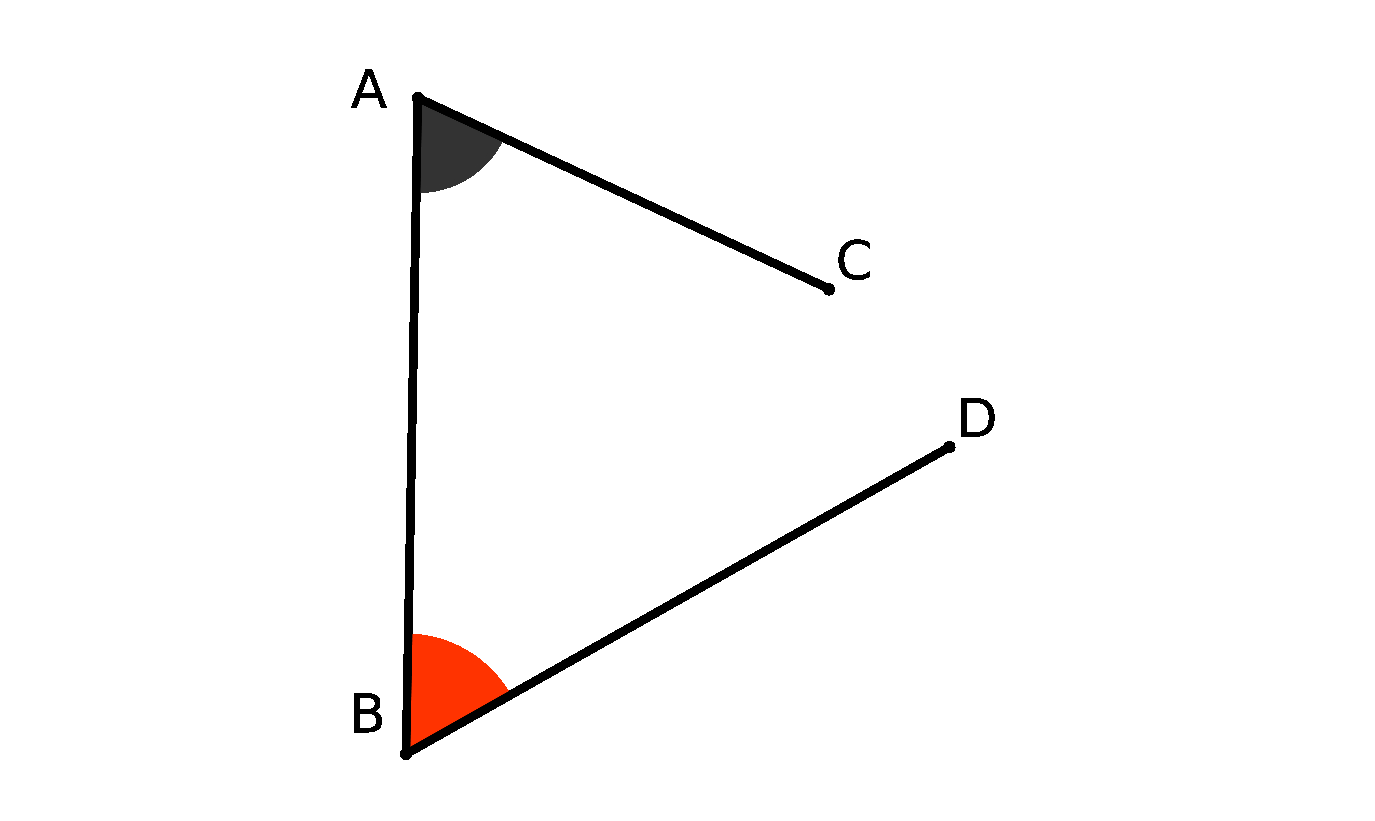
\includegraphics[scale=0.4]{figures/Postulat5.eps}\

 
\textit{Commentaire: les droites AC et BD coupent la droite AB en faisant des angles dont la somme est inférieure à deux droits.} \
 
\textit{c'est donc le postulat que l'on va essayer de démontrer pendant plus de deux mille ans! 
}\\



\textbf{Postulat 6:} et que deux droites n'entourent pas un domaine.\\



 
\textit{Commentaire: cela implique que deux droites ayant deux points communs sont égales. On va voir par la suite que c'est un postulat important.} \\


\section{Les axiomes:}

Les grecs appellent les axiomes "notions communes", c'est-à-dire des affirmations indémontrables, qui vont de soi (attitude peu mathématique!).\\

\textbf{axiome 1:} les chose égales à une même chose sont égales entre elles.\\



 
\textit{Commentaire: de quelles choses parle-t-on? } \\

\textbf{axiome 2:} et s'il est ajouté des chose égales à des choses égales les tout  seront égaux.\\



 
\textbf{axiome 3:} et s'il est retranché des chose égales à des choses égales les restes  seront égaux.\\



 
\textbf{axiome 4:} et s'il est ajouté des chose égales à des choses inégales les tout  seront inégaux.\\

\textbf{axiome 5:} et s'il est retranché des chose égales à des choses inégales les restes  seront inégaux.\\

\textbf{axiome 6:} et les choses doubles d'une même chose sont égales entre elles.\\



\textbf{axiome 7:} et les choses moitié d'une même chose sont égales entre elles.\\

\textbf{axiome 8:} et les choses qui s'ajustent entre elles sont égales entre elles.\\
 
 \textbf{axiome 9:} et le tout est plus grand que la partie.\\
 
\textit{Commentaire:} naturellement, c'est faux dans un ensemble infini, mais pour les grecs un tout infini n'a pas de sens. \\



\section{Les théorèmes:}

Nous énoncerons les théorèmes du livre 1 des Eléments d'Euclide en indiquant ceux qui nécessitent P5 ou P6 et démontrerons ceux aussi ceux dont la démonstration est insuffisante.\\

\subsection{Livre 1: théorèmes ne faisant pas intervenir P5.}


\textbf{théorème 1: construire un triangle équilatéral.}\\

\textit{Démonstration:} On trace une droite AB (P1).\

 On construit le cercle C de centre A et de rayon AB (P3)\
 
  puis le cercle C' de centre B et de rayon AB.\

Alors les deux cercles se coupent en un point C. Et le triangle ABC est équilatéral.\\

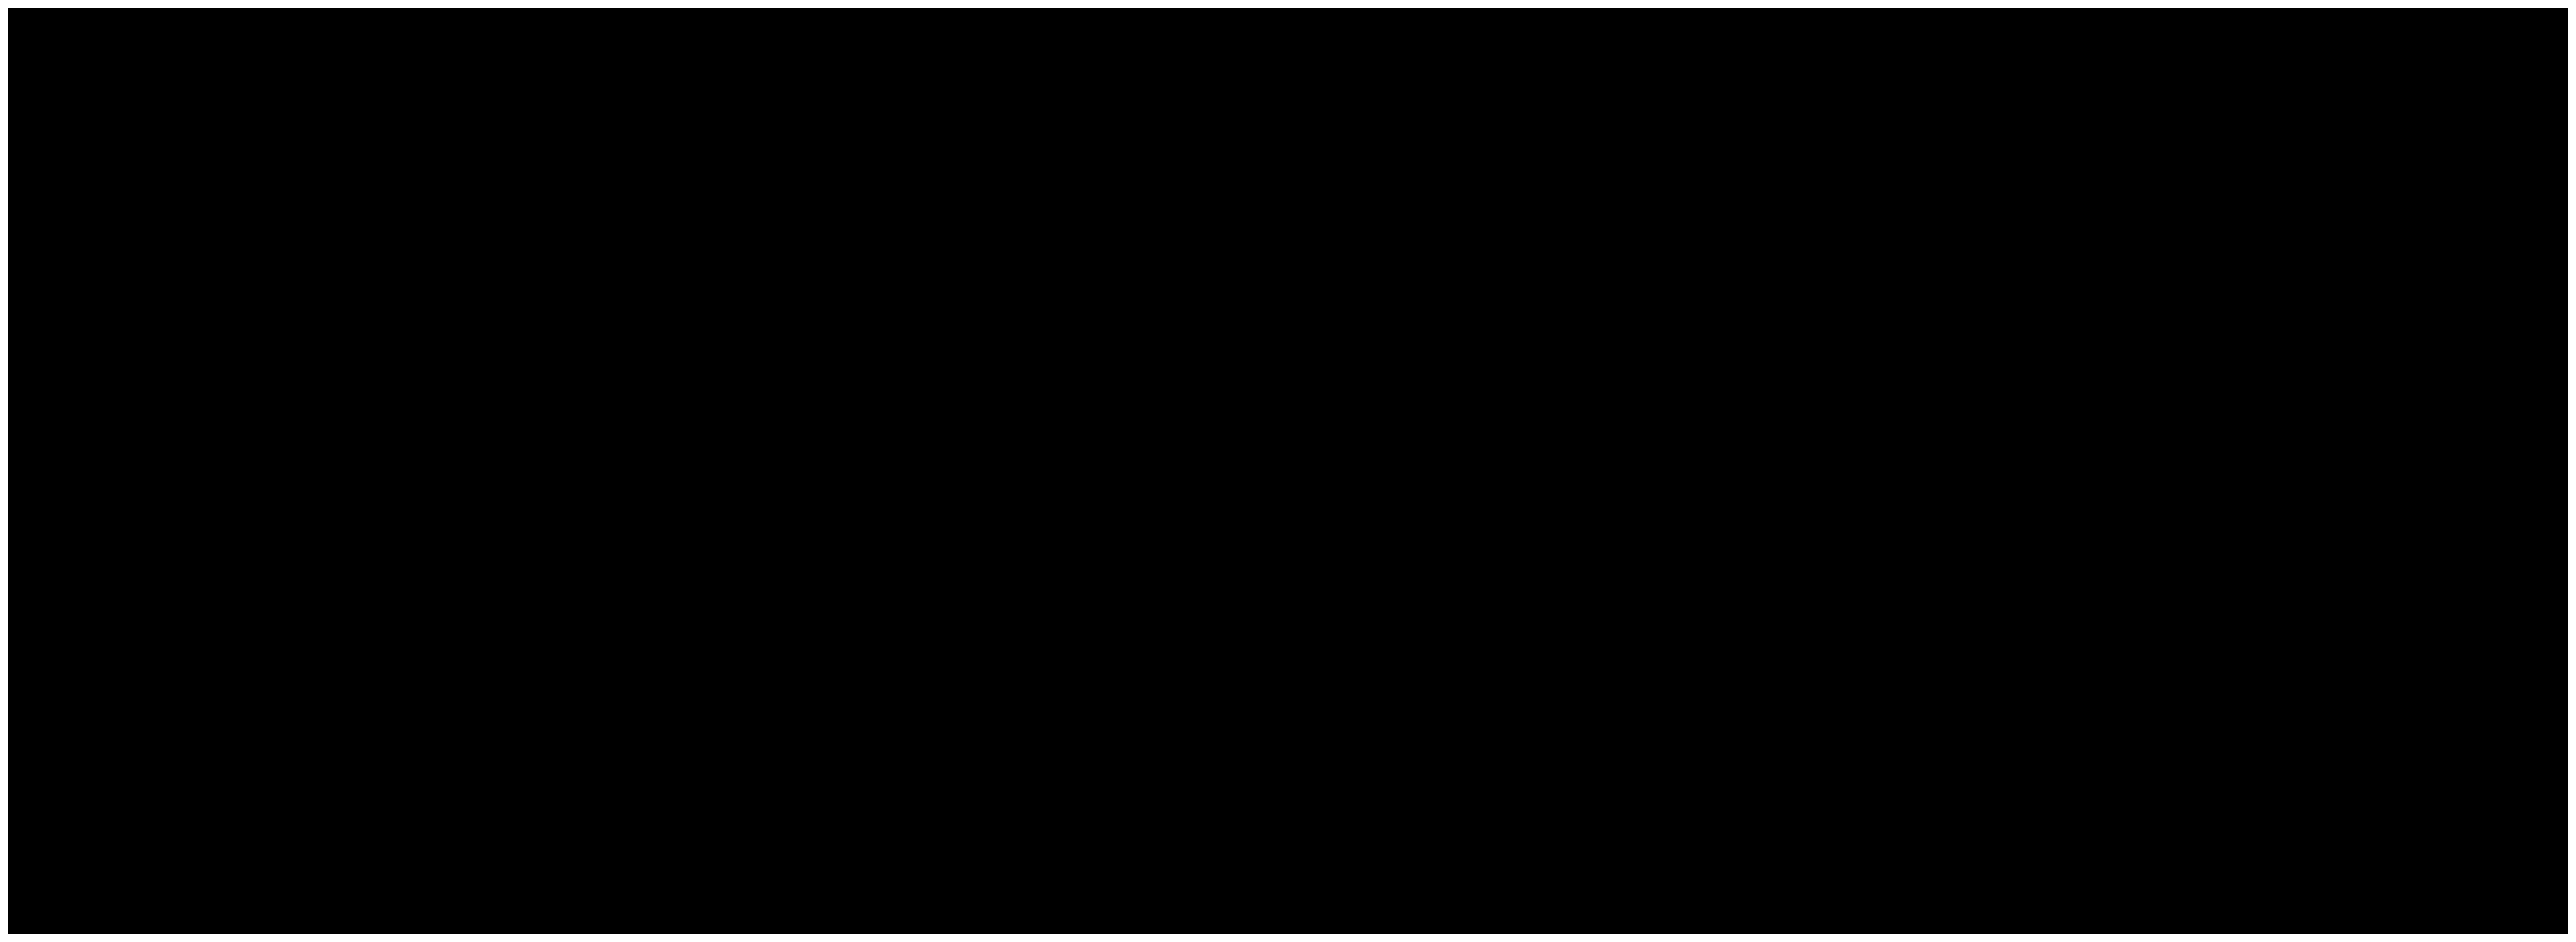
\includegraphics[scale=0.2]{figures/th1.eps}\\ 


\textit{Commentaire:} On "voit" que les cercles se coupent, mais rien dans les définitions ou postulats ou axiomes ne nous le dit. Il faudrait    donc ajouter un nouveau postulat, P7, suivant:\

P7: un cercle partage le plan en deux domaines et si on prend un point dans le cercle et un autre à l'extérieur, toute ligne joignant les deux points coupe le cercle en un point.\\

Ainsi, on pourra affirmer que C' coupe C.\\

\textbf{théorème 2: d'un point donné A, placer une droite égale à une droite donnée BC.}\\

\textit{Démonstration:} On construit le triangle équilatéral ABD (th1.1),\

 puis le cercle de centre B et de rayon BC (P1). DB coupe ce cercle en E (quitte à prolonger DB (P2)).\

 Puis le cercle de rayon DE qui coupe AD en F (P1).\
 
  On a alors $BE=BC$, $DE=DF$, $DA=DB$. Donc $AF=BE=BC$.\\
 
 

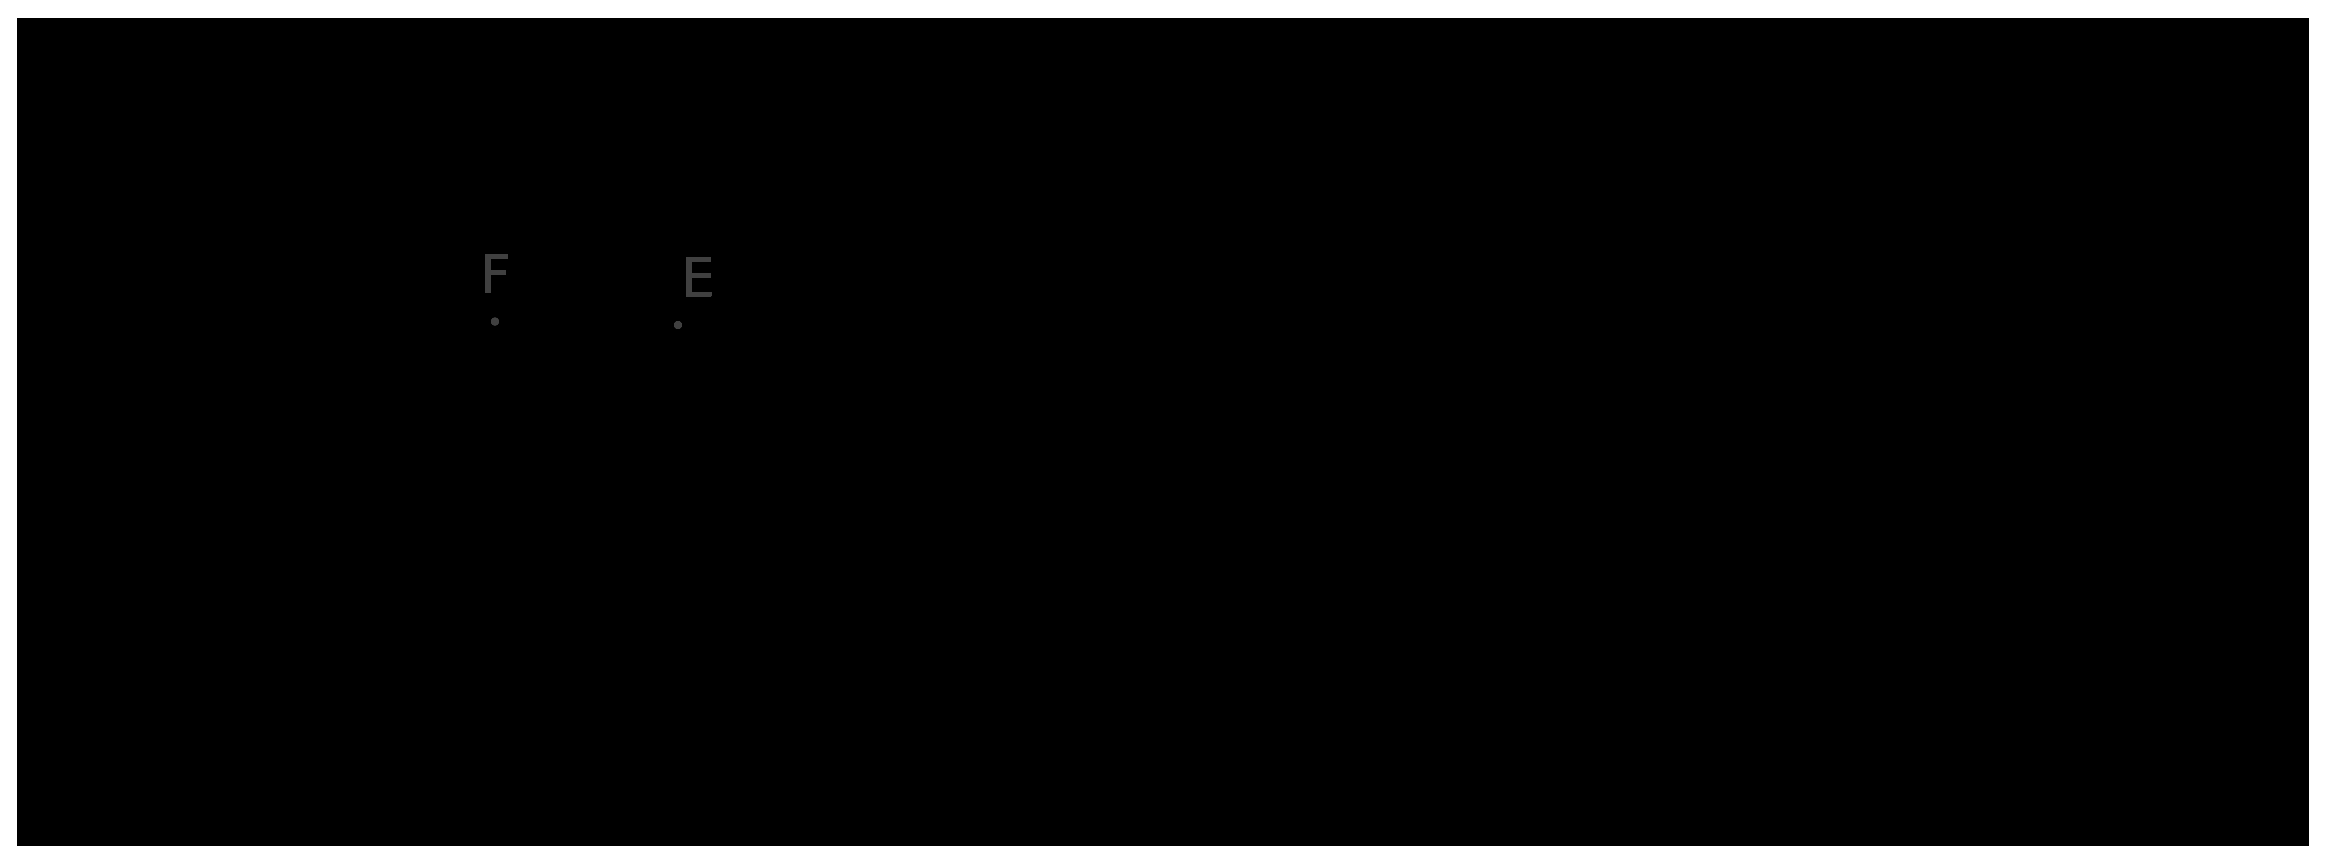
\includegraphics[scale=0.3]{figures/th2.eps}\\

\textit{Commentaire:} on se sert manifestement de la figure. Pour être rigoureux, il faudrait prendre tous les cas de figures: par exemple: que se passe-t-il si $BC>BD$? On s'en sort mais il faudrait le faire!\

En fait, DB coupe le cercle en deux points: la démonstration donne-t-elle le même résultat? oui, mais encore faudrait-il le faire.\\

\textbf{théorème 3: on donne deux droites de longueur inégale, ôter de la plus grande une droite égale à la plus petite.}\\

\textbf{théorème 4: si deux triangles ont un angle égal et les côtés qui entourent cet angle égaux alors les bases des triangles sont égales. Alors les triangles seront égaux et les angles restants aussi.}\\

\textit{commentaire} ici P6 intervient! 
 

 
 
  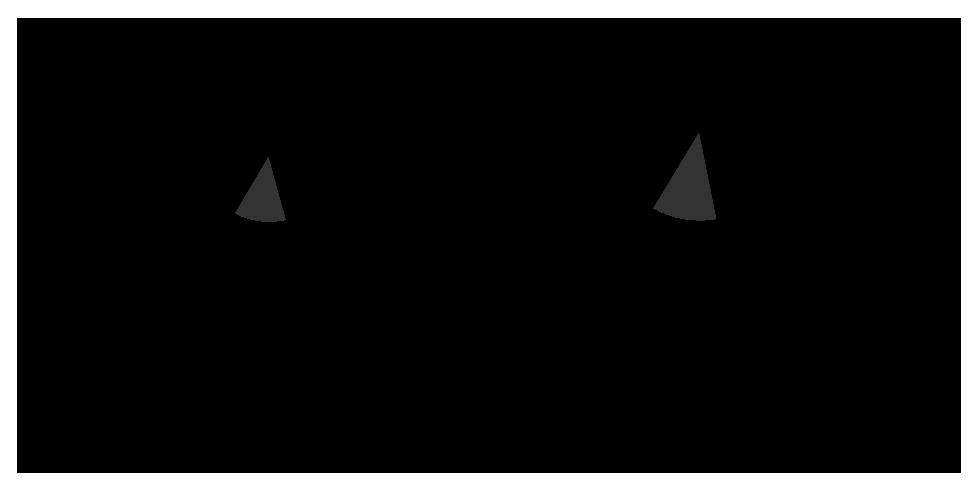
\includegraphics[scale=0.5]{figures/LIVRE1&4.eps} \
  
 \textit{démonstration:} Soient deux triangles ABC et DEF tels que $CA=DF$, $CB=FE$ et $A\hat{C}B=D\hat{F}E$.\
 
 Appliquons C sur F puis CA sur FD\
 
 \textit{comment fait-on pour appliquer une figure sur une autre? on a à priori aucun outil dans Euclide pour le faire!}.\
 
  Alors A s'applique sur D. \
 
 Mais CA s'appliquant sur FD, CB s'appliquera sur FD puisque $A\hat{C}B=D\hat{F}E$ donc B s'appliquera sur E puisque $CB=FE$.\
 
 A s'applique sur D et B sur E donc AB s'applique sur DE sinon deux droites entoureraient un domaine ce qui contredit P6.\\
 
 \textit{Commentaire: Si on enlève de GN le postulat 6 cela signifiera que le th 4 sera faux lorsque deux points définiront plus de deux droites, mais juste sinon}.\\
 
 \textit{Pour Euclide les triangles étant ajustables, ils sont égaux. Pour nous ils sont isométriques ou congruents}.\\
  
 \textbf{Théorème 5: dans un triangle isocèle les angles à la base sont égaux.}\\
 
 \textit{Commentaire:} la démonstration dépend de th4 donc de P6.\\
 
 
  \textbf{Théorème 6: si un triangle a deux angles égaux entre eux les côtés qui sous tendent les angles sont égaux.}\\
  
  \textit{Commentaire:} la démonstration dépend de th4 donc de P6.\\
 
  
 \textbf{Théorème 7: sur une même droite,  à partir de deux points situés du même côté de cette droite il n'est pas possible de tracer deux droites égales à deux autres droites, chacune à chacune, ayant les mêmes extrémités que ces autres.}\\
 
 
 
 
  
 
 
    
 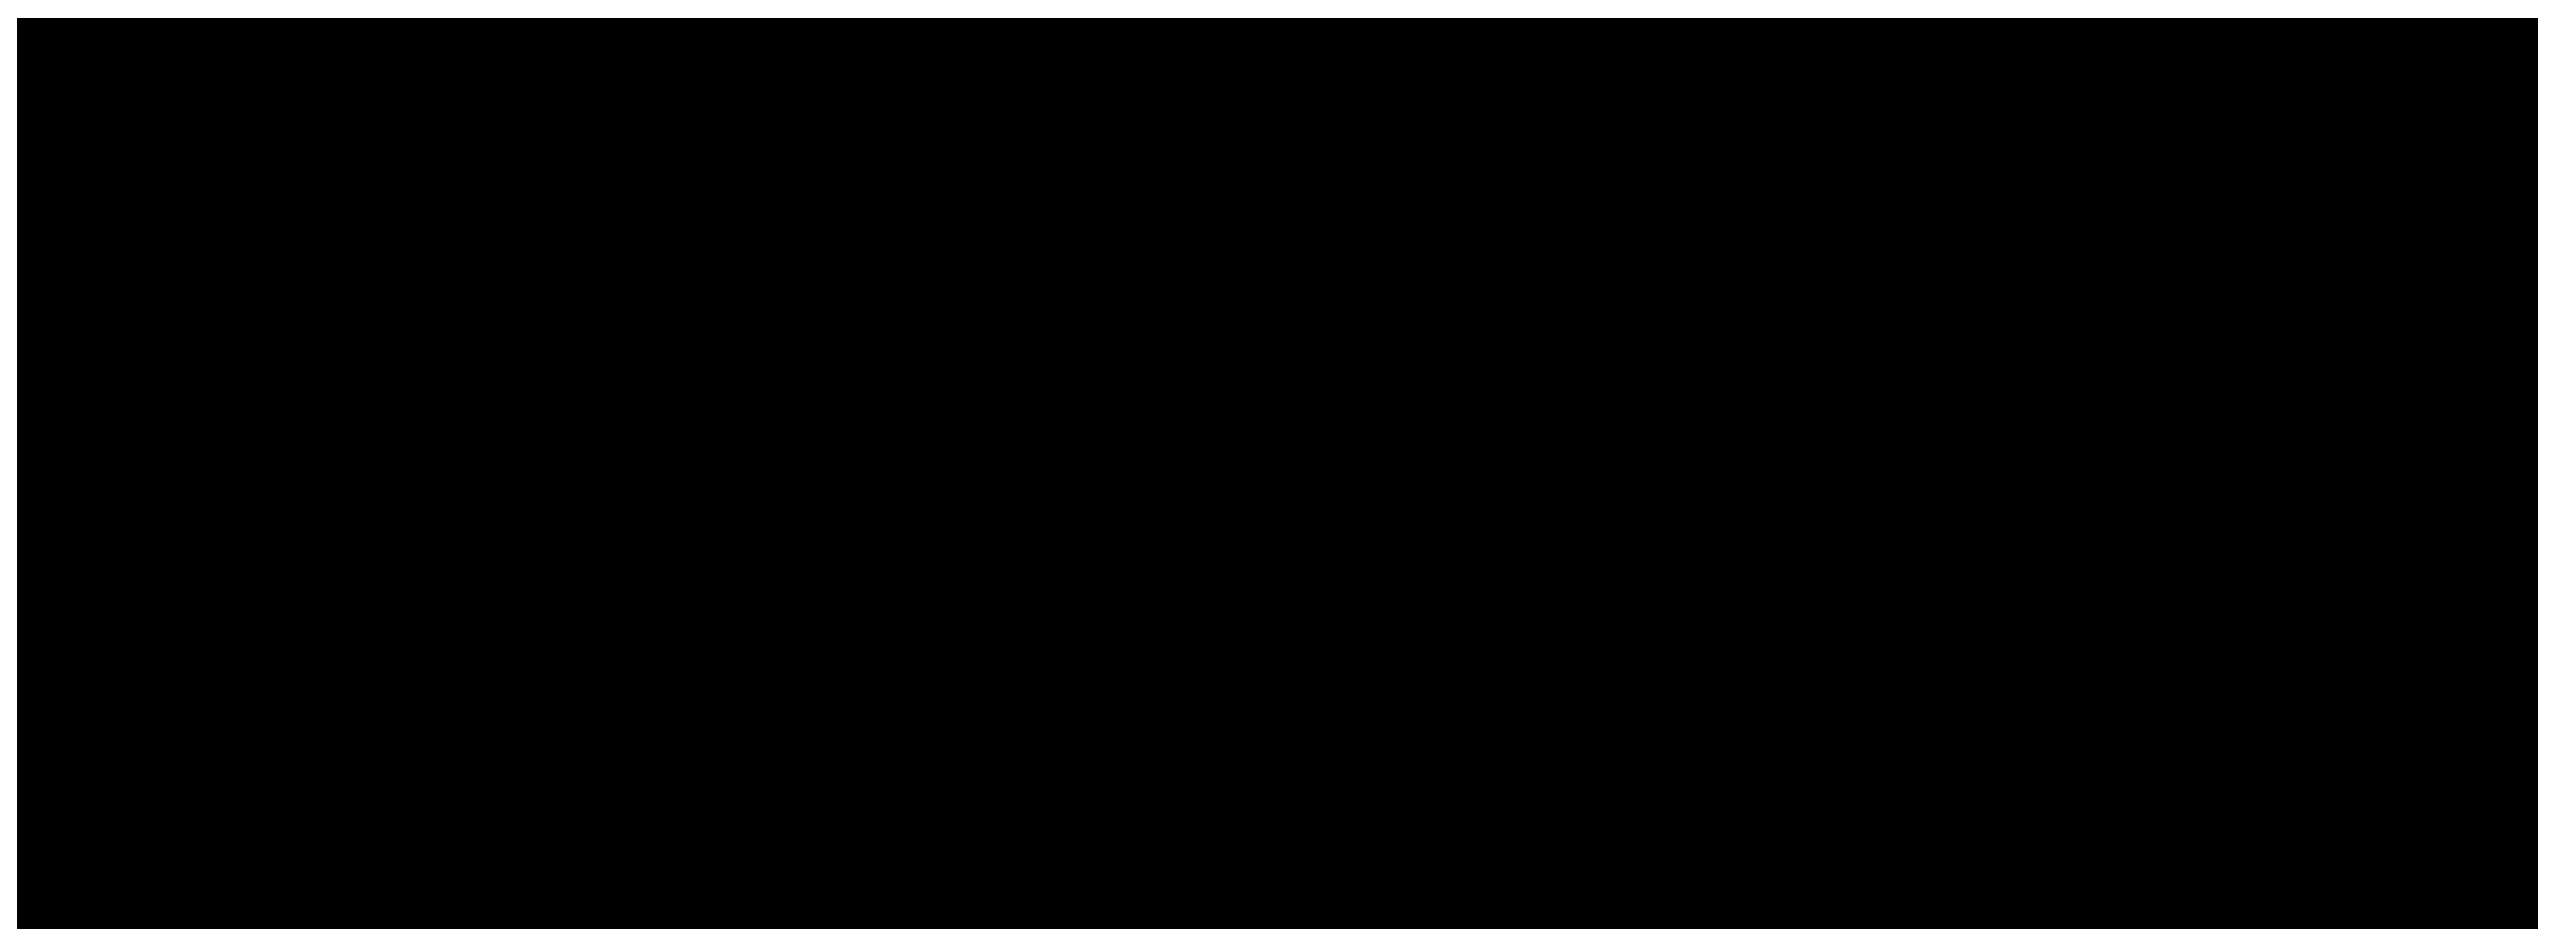
\includegraphics[scale=0.2]{figures/th7.eps} \\
 
 \textit{commentaire:} Cela signifie que si on prend une droite AB, deux points situés du même côté de AB et que l'on trace les droites CA et CB, on ne peut pas tracer deux droites issues de D telles que $CA=DA$ et $DB=CB$. \\
 
 Il manque là un postulat que nous nommerons \textbf{P8}: une droite partage le plan en deux régions ayant comme frontière la droite et si l'on prend un point de part et d'autre de la droite, la droite joignant les deux points coupe la droite.\
 
 Avec ce postulat il est possible de choisir deux points du même côté de AB.\\
 
 \textbf{Théorème 8: si deux triangles ont deux côtés égaux, chacun à chacun, et la base égale à la base, alors ils auront un angle égal à un angle égal, celui qui est compris entre les côtés égaux.}\\
 
 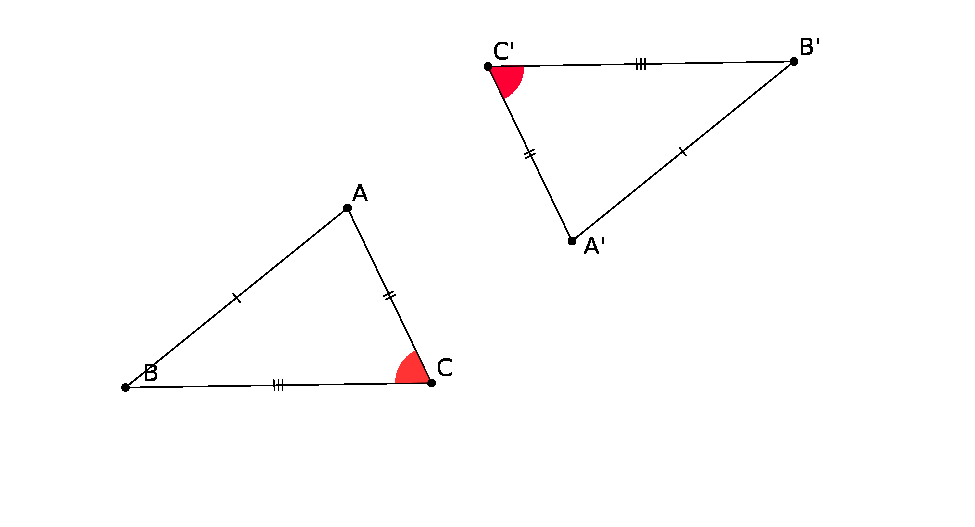
\includegraphics[scale=0.7]{figures/euc.eps} \\
 
 \textbf{Théorème 9: couper un angle rectiligne en deux.}\\
 
 
 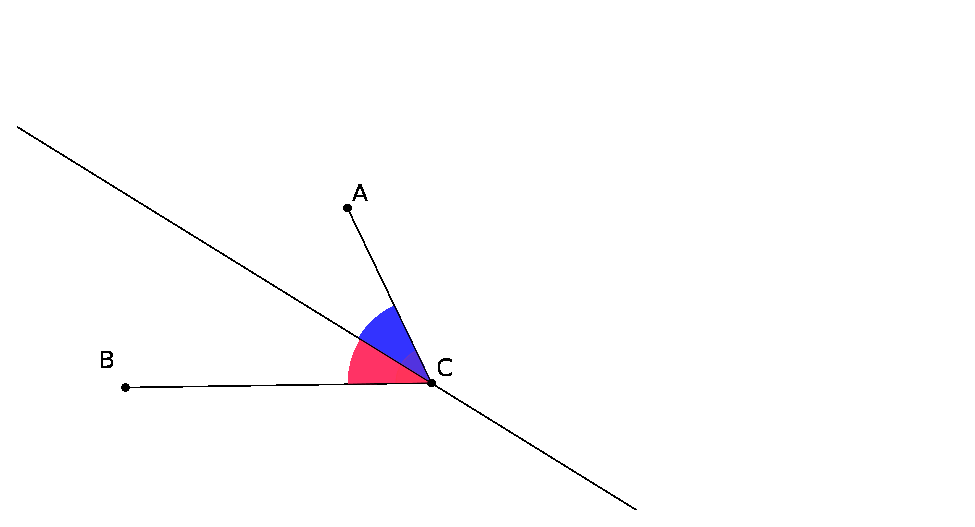
\includegraphics[scale=0.7]{figures/euc2.eps} \\
 
 
 \textbf{Théorème 10: couper une droite donnée en deux.}\\\\
 
 
 
 \textbf{Théorème 11: à une droite donnée, d'un point donné de cette droite, mener une ligne droite avec des angles droits.}\\
 
     
 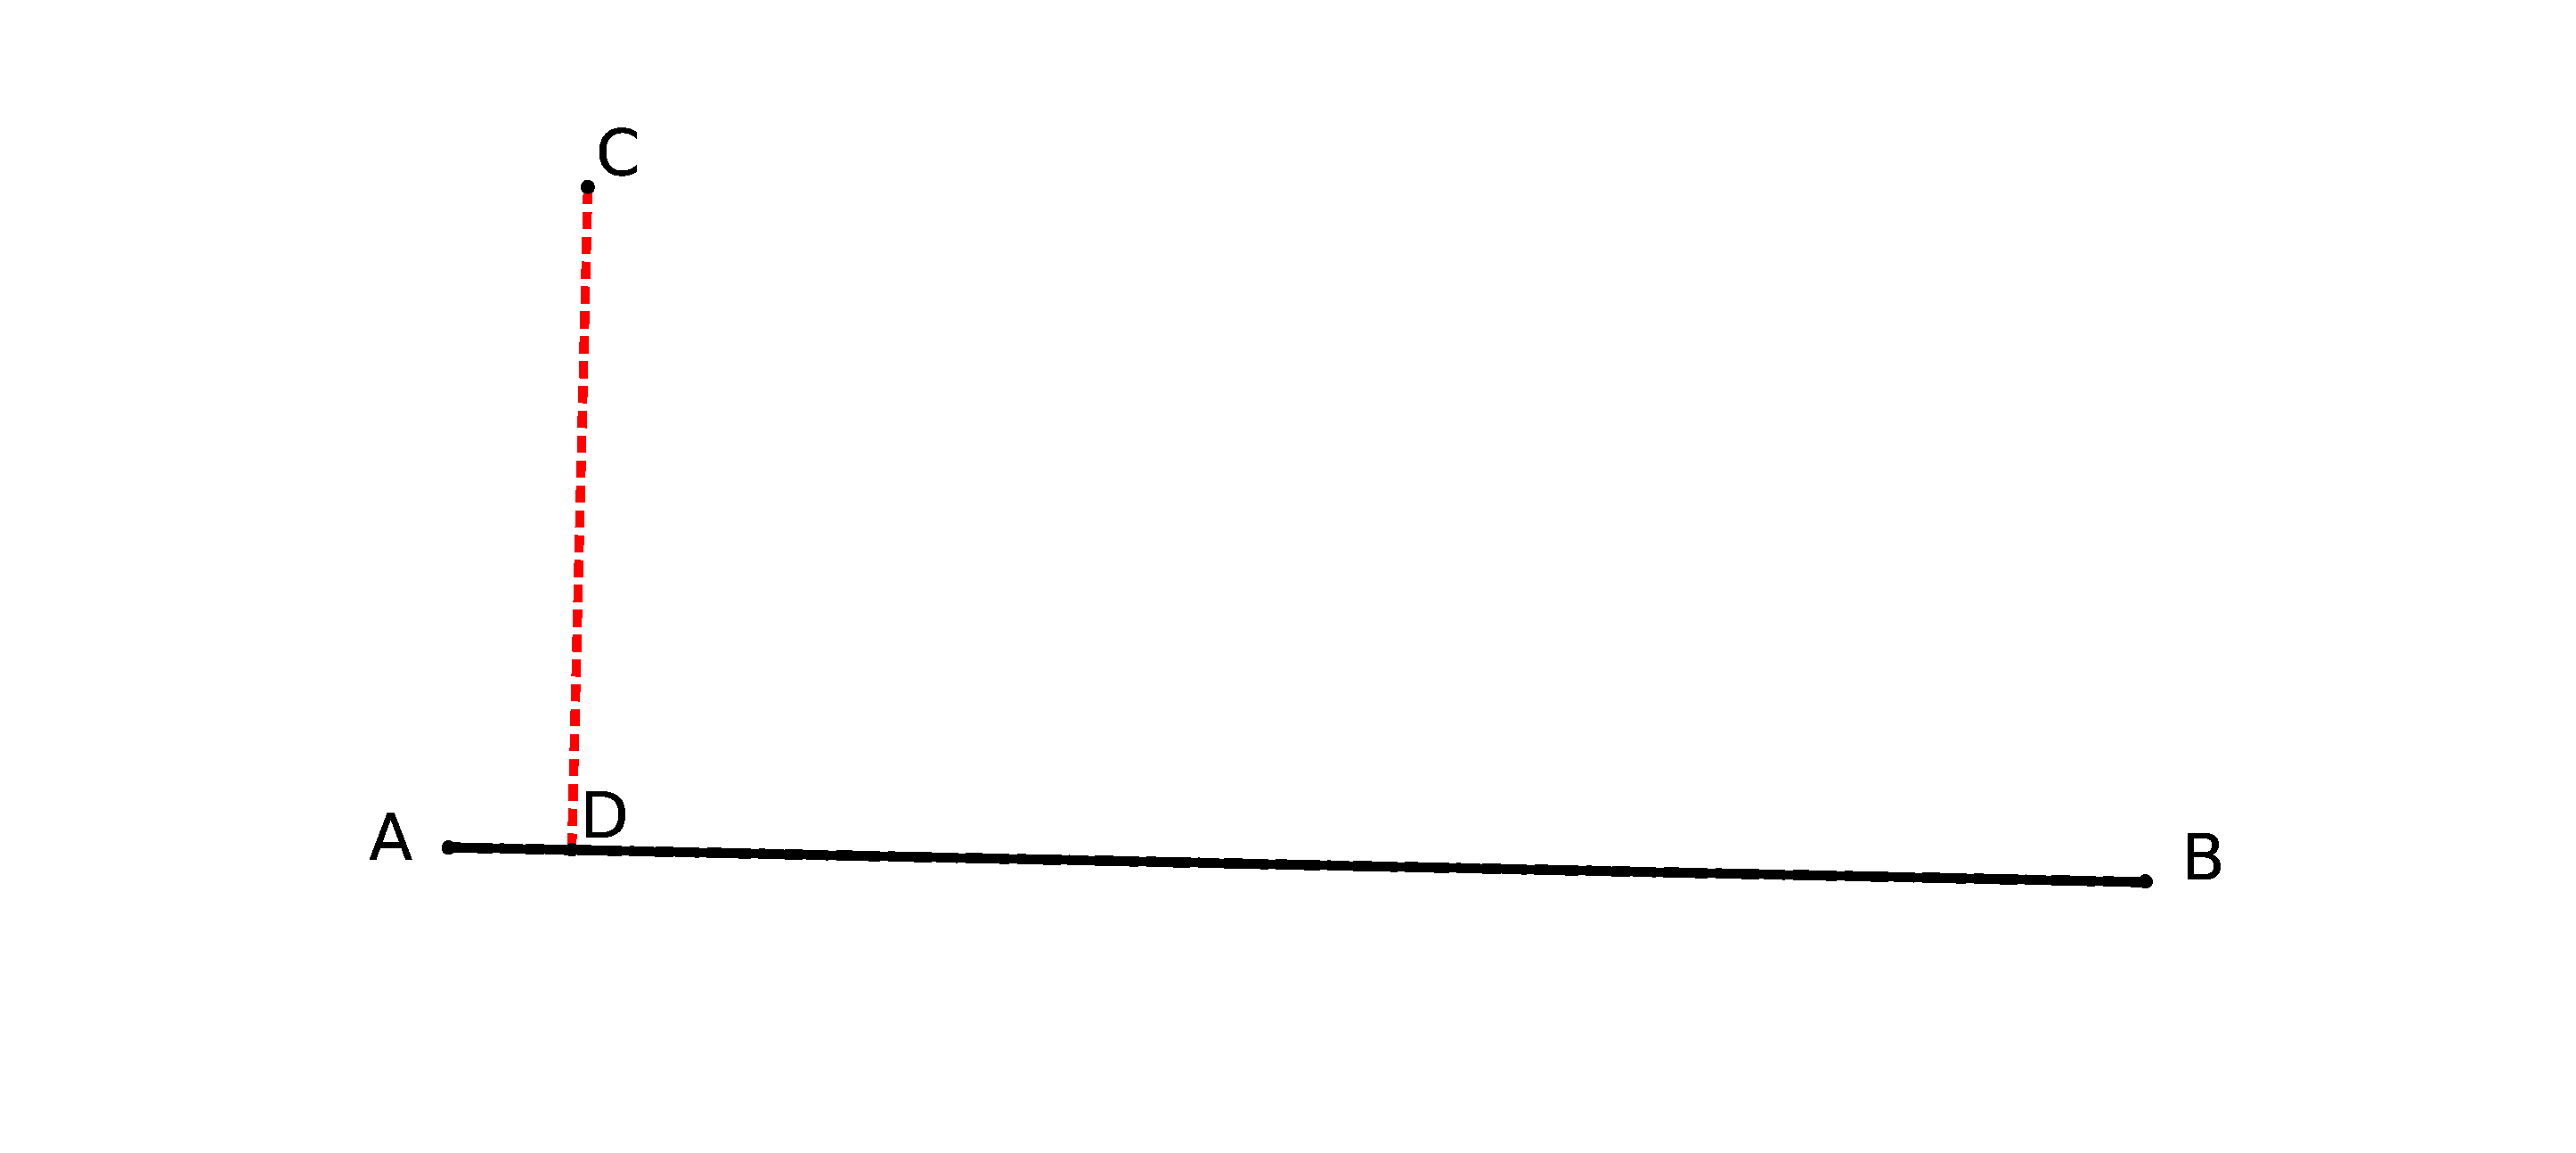
\includegraphics[scale=0.2]{figures/th11.eps} \\
 
 \textbf{Théorème 12:  à une droite donnée, d'un point donné n'appartenant pas à cette droite, mener une ligne droite avec des angles droits.}\\
 
 \textbf{Théorème 13: si une droite tombant sur une droite fait deux angles, soit ils sont droits, soit ils font ensemble deux droits.}\\
 
 \textbf{Théorème 14: si à partir d'une droite et d'un point de cette droite, deux droites non situées du même côté, font ensemble deux angles égaux à deux droits, ces deux droites sont situées dans la même direction.}\\
 
      
 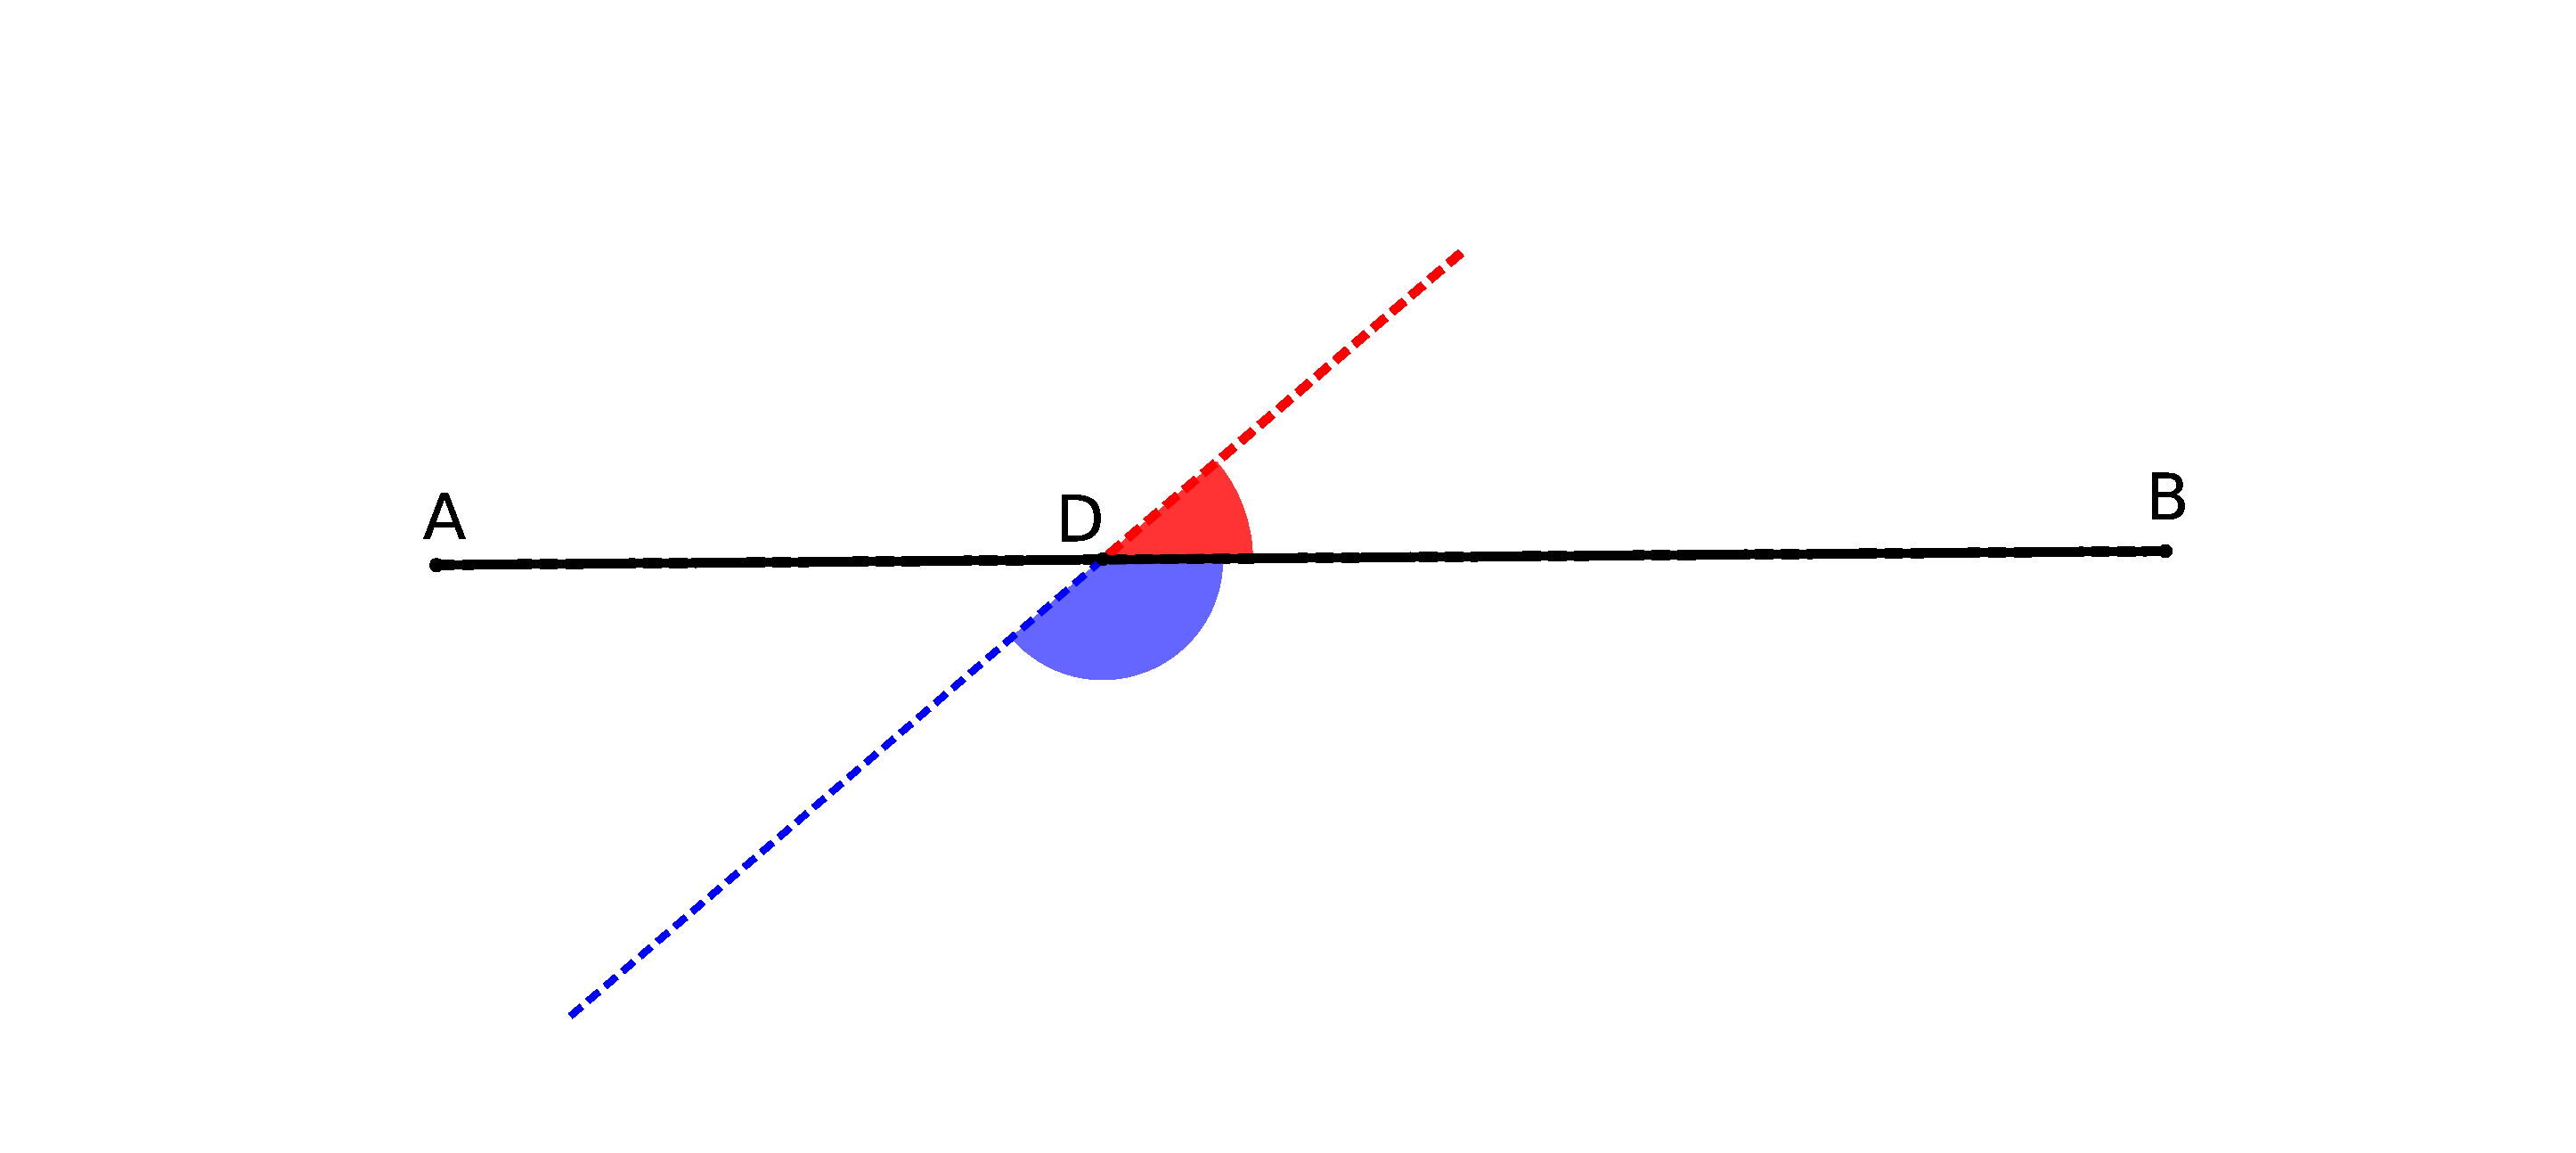
\includegraphics[scale=0.2]{figures/th14.eps} \\
 
 
 \textbf{Théorème 15: si deux droites se coupent entre elles, elles font des angles égaux au sommet.}\\
 
 \textbf{Théorème 16: le côté d'un triangle étant prolongé, l'angle extérieur est plus grand que chacun des angles opposés et extérieurs.}\\
  
  $\hat{ACD}$ est l'angle extérieur, $\hat{ABC}$ l'angle intérieur et $\hat{BAC}$ l'angle opposé.\\
  
   
   
   \textit{démonstration:} Soit E le milieu de AC (th10)\
   
    et soit F tel que $BE=EF$ (th2).\
   
   On a: $AE=EC$, $BE=EF$ et $\hat{AEB}=\hat{FEC}$ (Th15.1)\
   
   donc les triangles AEB et FEC sont égaux (th4).\
   
    Donc les angles $\hat{ACF}$ et $\hat{BAC}$ sont égaux (th4).\
   
   
    B, E et C ne sont pas alignés donc F ne peut pas être sur CD. Sinon BF et BD seraient deux droites distinctes entourant un domaine et cela contredirait P6.\
    
     Donc   $\hat{ACD}>\hat{ACF}$. Donc $\hat{ACD}>\hat{BAC}$. CQFD.\
    Même démonstration pour l'angle ABC.\\
    
    
   
   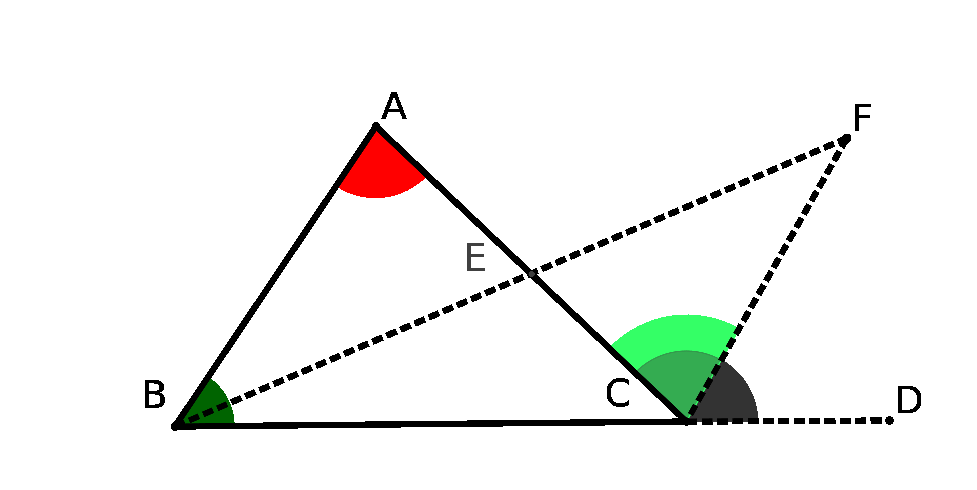
\includegraphics[scale=0.5]{figures/LIVRE1&16.eps} \\
   
  \textit{Commentaire:} on voit bien que P6 joue un rôle ici important, que ce soit par l'application de th4 ou par le fait que A, C et F ne sont pas alignés.\
  
  De plus on peut remarquer que l'on a doublé la longueur de BE: est-ce possible? P2 nous permet de "sortir continûment" la droite BE d'elle-même, mais d'être doublée, ce n'est pas dit.\\
  
  
  
  \newpage \textbf{théorème 17:les deux angles d'un triangle, pris de manière quelconque, sont plus petits que deux droits.}\\
  
 \textit{Commentaire:} C'est une conséquence du théorème précédent donc de P6.\\
 
 
\textbf{théorème 18:  dans tout triangle, un plus grand côté sous tend un plus grand angle.}\\
 
 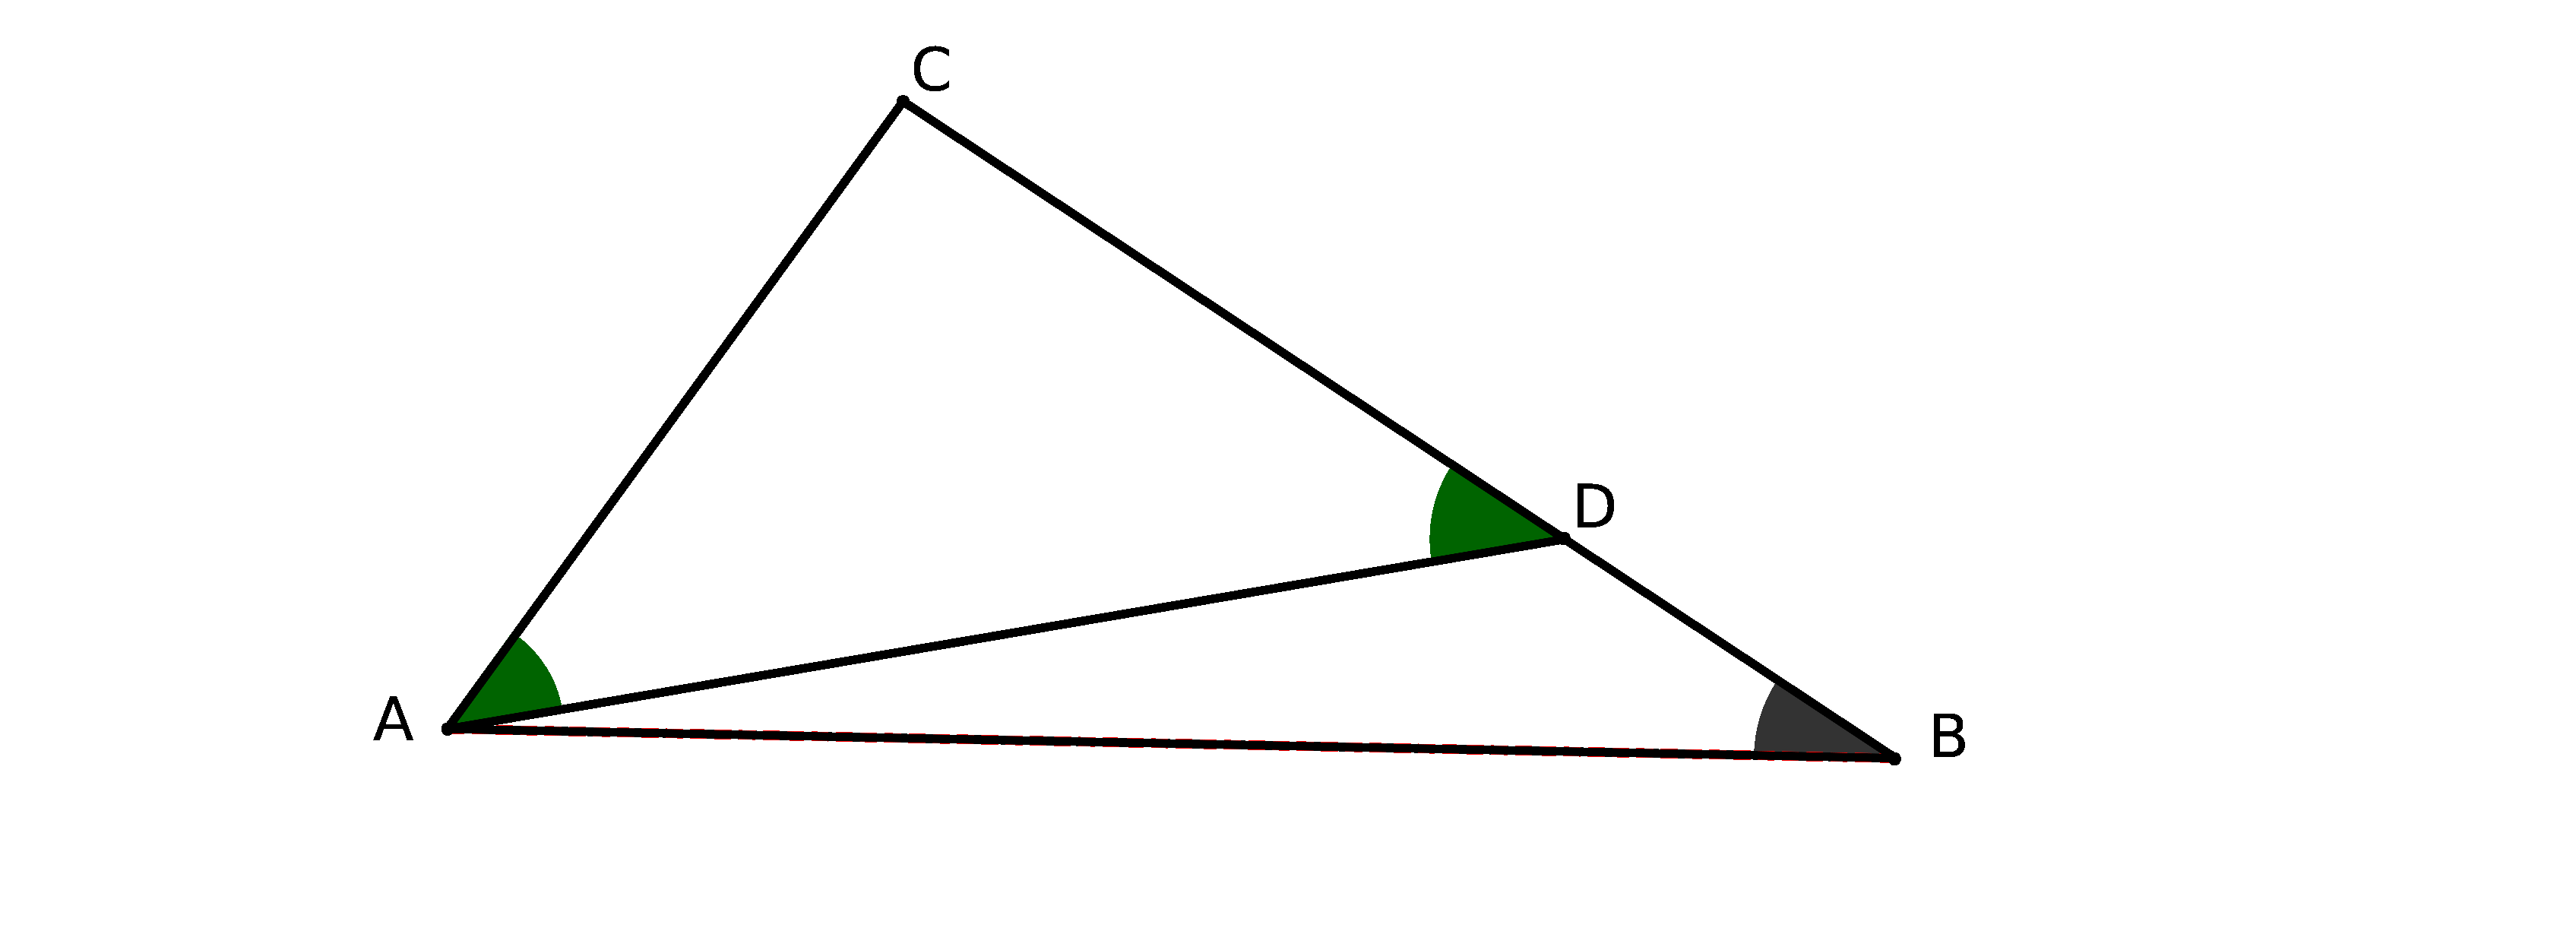
\includegraphics[scale=0.2]{figures/th18.eps}\\ 
 
\textit{Démonstration:} soit ABC un triangle dans lequel $CB>CA$. Soit D le point de CB tel que $CD=CA$ (Th2.1).\

 Alors $\hat{CAD}=\hat{CDA}$ (th5.1).\
 
  Comme $\hat{CDA}$ est l'angle extérieur du triangle ADB on a: $\hat{CBA}<\hat{CDA}$ (th.16.1) \\

\textit{commentaire: C'est donc une application de th 16.1 donc de P6}.\\

 \textbf{Théorème 19:  dans tout triangle, un  côté  qui sous tend un angle plus grand est plus grand qu'un côté qui sous tend un angle plus petit.}\\
 
 \textit{commentaire: C'est aussi une application de th 16 donc de P6}.\\
 
 \textbf{Théorème 20: dans tout triangle deux des côtés, pris de toute manière, sont, ensemble, plus grands que celui qui reste.}\\
 

 
 \textit{commentaire: il s'agit de l'inég\textbf{alité triangulaire}. Nous verrons que sur une sphère ce n'est pas forcément vrai!}
 
 \textit{C'est aussi une application de th 16 donc de P6}.\\
 
\newpage  \textbf{Théorème 21: si des extrémités d'un côté d'un triangle on construit intérieurement deux droites, ces deux droites seront plus petites que les deux côtés restants du triangle mais elles formeront un angle plus grand.}\\

Dans la figure ci-dessous cela signifie que $DA+DB<CA+CB$.\\

  
 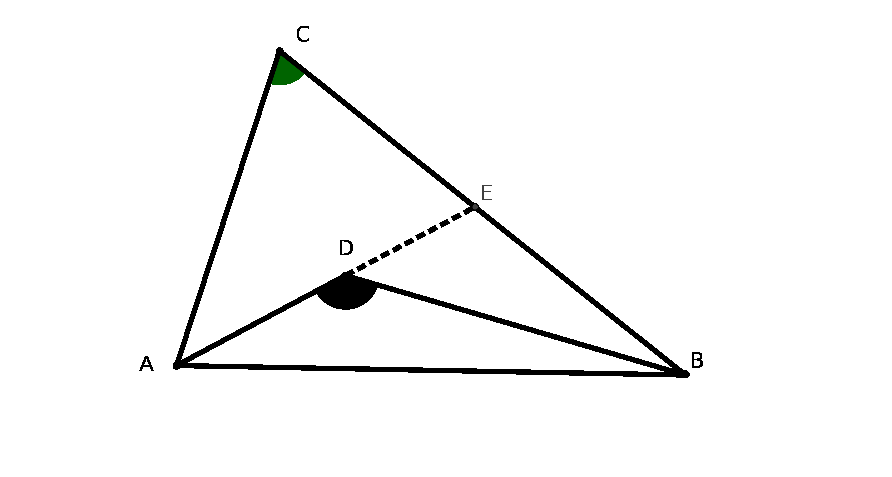
\includegraphics[scale=0.5]{figures/th21.eps}\\\
  
  
 \textit{Démonstration:}\ 
  
 A. 1. Soit E le point d'interchapter de AD et BC (cf commentaire).\medskip 
  
  2. On a $AC+EC>AE $ donc $AC+EC+EB>AE+EB $ (A2) donc $AC+CB>AE+EB$ donc $AC+CB>AD+(DE+EB)$ \medskip 
  
   
  3. Et on a  $DE+EB>BD$.\medskip 
    
  4. Donc  $AC+CB>AD+(DE+EB)>AD+BD $ donc $AC+CB>AD+DB$ \medskip 
  
  B. La démonstration sur les angles ne pose aucun problème.\\
  
  
  
 
     
\textit{Commentaire: chacune des étapes, 2, 3 ou 4 de la démonstration est justifiée par des axiomes ou théorèmes démontrés avant le théorème 21 et dépendent de P6 mais... l'étape 1 n'est pas justifiée: en effet, aucun postulat, aucun axiome ni aucun théorème précédent ne permet d'affirmer que la droite qui joint un sommet à un point intérieur à un triangle coupe le côté opposé. La droite AD pourrait être prolongée continûment sans couper aucun côté: difficile à imaginer mais pourquoi pas? Il faudrait poser ce résultat   en postulat! \\
On voit là, malgré toute la volonté de rigueur d'Euclide, qu'il se laisse, que nous nous laissons, influencer par ce que l'on voit!}\\

 \textbf{Théorème 22: à partir de trois droites construire un triangle (deux des droites étant plus grandes que la troisième).}\\
 
  
  \newpage \textbf{théorème 23: à partir d'une droite donnée et d'un point de cette droite construire un angle rectiligne égal à un angle rectiligne donné.} \\
  
 
 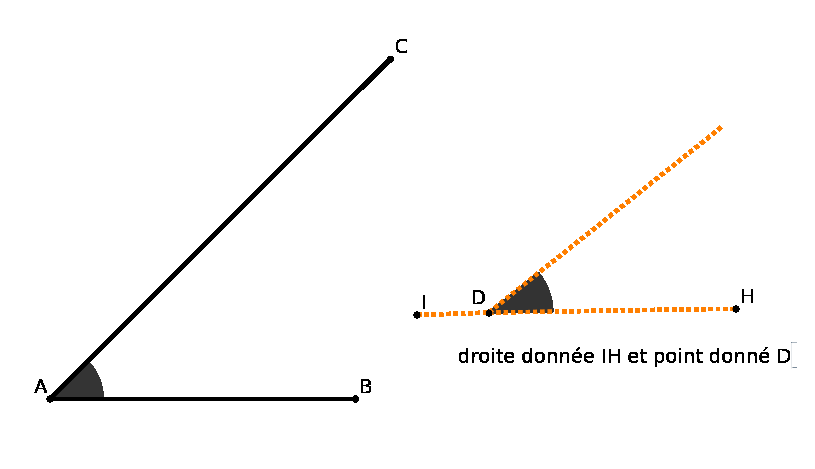
\includegraphics[scale=0.7]{figures/LIVRE1&23.eps} \\
 
\textbf{théorème 24: si deux triangles ont deux côtés égaux à deux côtés, chacun à chacun, et s'ils ont un angle plus grand qu'un angle, celui qui est entouré par les côtés égaux, alors la base est plus grande que la base.} \\

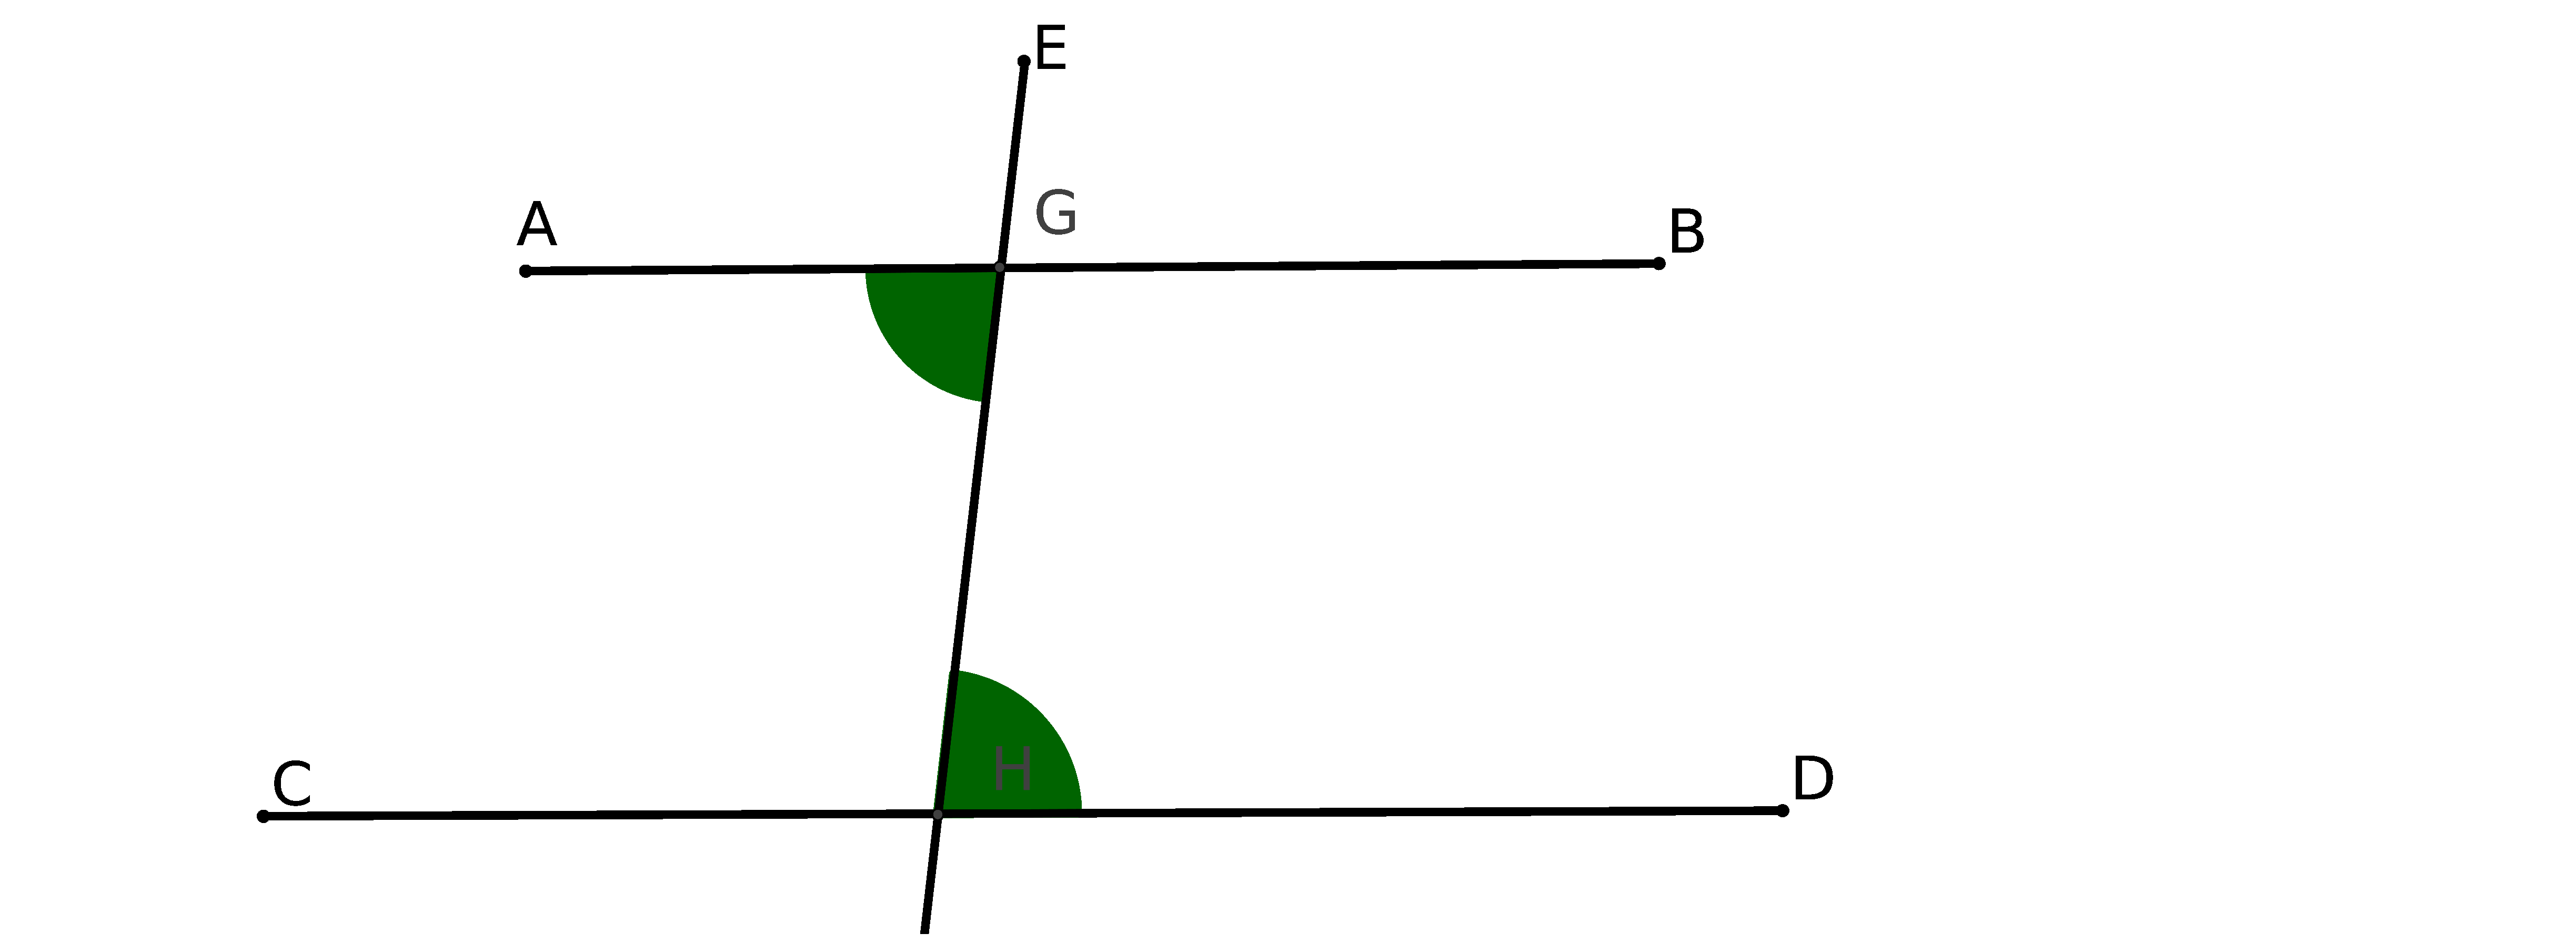
\includegraphics[scale=0.2]{figures/th24.eps} \\

\textit{Démonstration:} Soient les triangles ABC et DIH tels que $CA=DH$, $CB=HJ$ et $\hat{ACB}>\hat{DHI}$.\

On construit  le triangle HDJ égal au triangle ACB (th 22.1).\

Alors $HI=HJ$ donc $\hat{HIJ}=\hat{HJI}$ donc $\hat{HIJ}>\hat{DJI}$.\

Mais $\hat{DIJ}>\hat{HIJ}$ donc $\hat{DIJ}>\hat{DJI}$ (th5.1) donc $DJ>DI$ donc $AB>DI$ (th 19.1).\\

\textit{Commentaire:} P6 est là aussi.\\


\newpage \textbf{Théorème 25: si deux triangles ont deux côtés égaux chacun à chacun et une base plus grande qu'une base alors un angle sera plus grand qu'un angle, celui qui est sous les côtés égaux.}\\

\textit{Commentaire:} c'est la réciproque du précédent.\\

  \textbf{théorème 26: si deux triangles ont deux angles égaux, chacun à chacun, et un côté égal à un côté alors les côtés restants sont égaux, chacun à chacun.}\\
  
   \textbf{Théorème 27: si une droite tombant sur deux droites fait des angles alternes égaux, les deux droites sont parallèles.}\\
  
  
  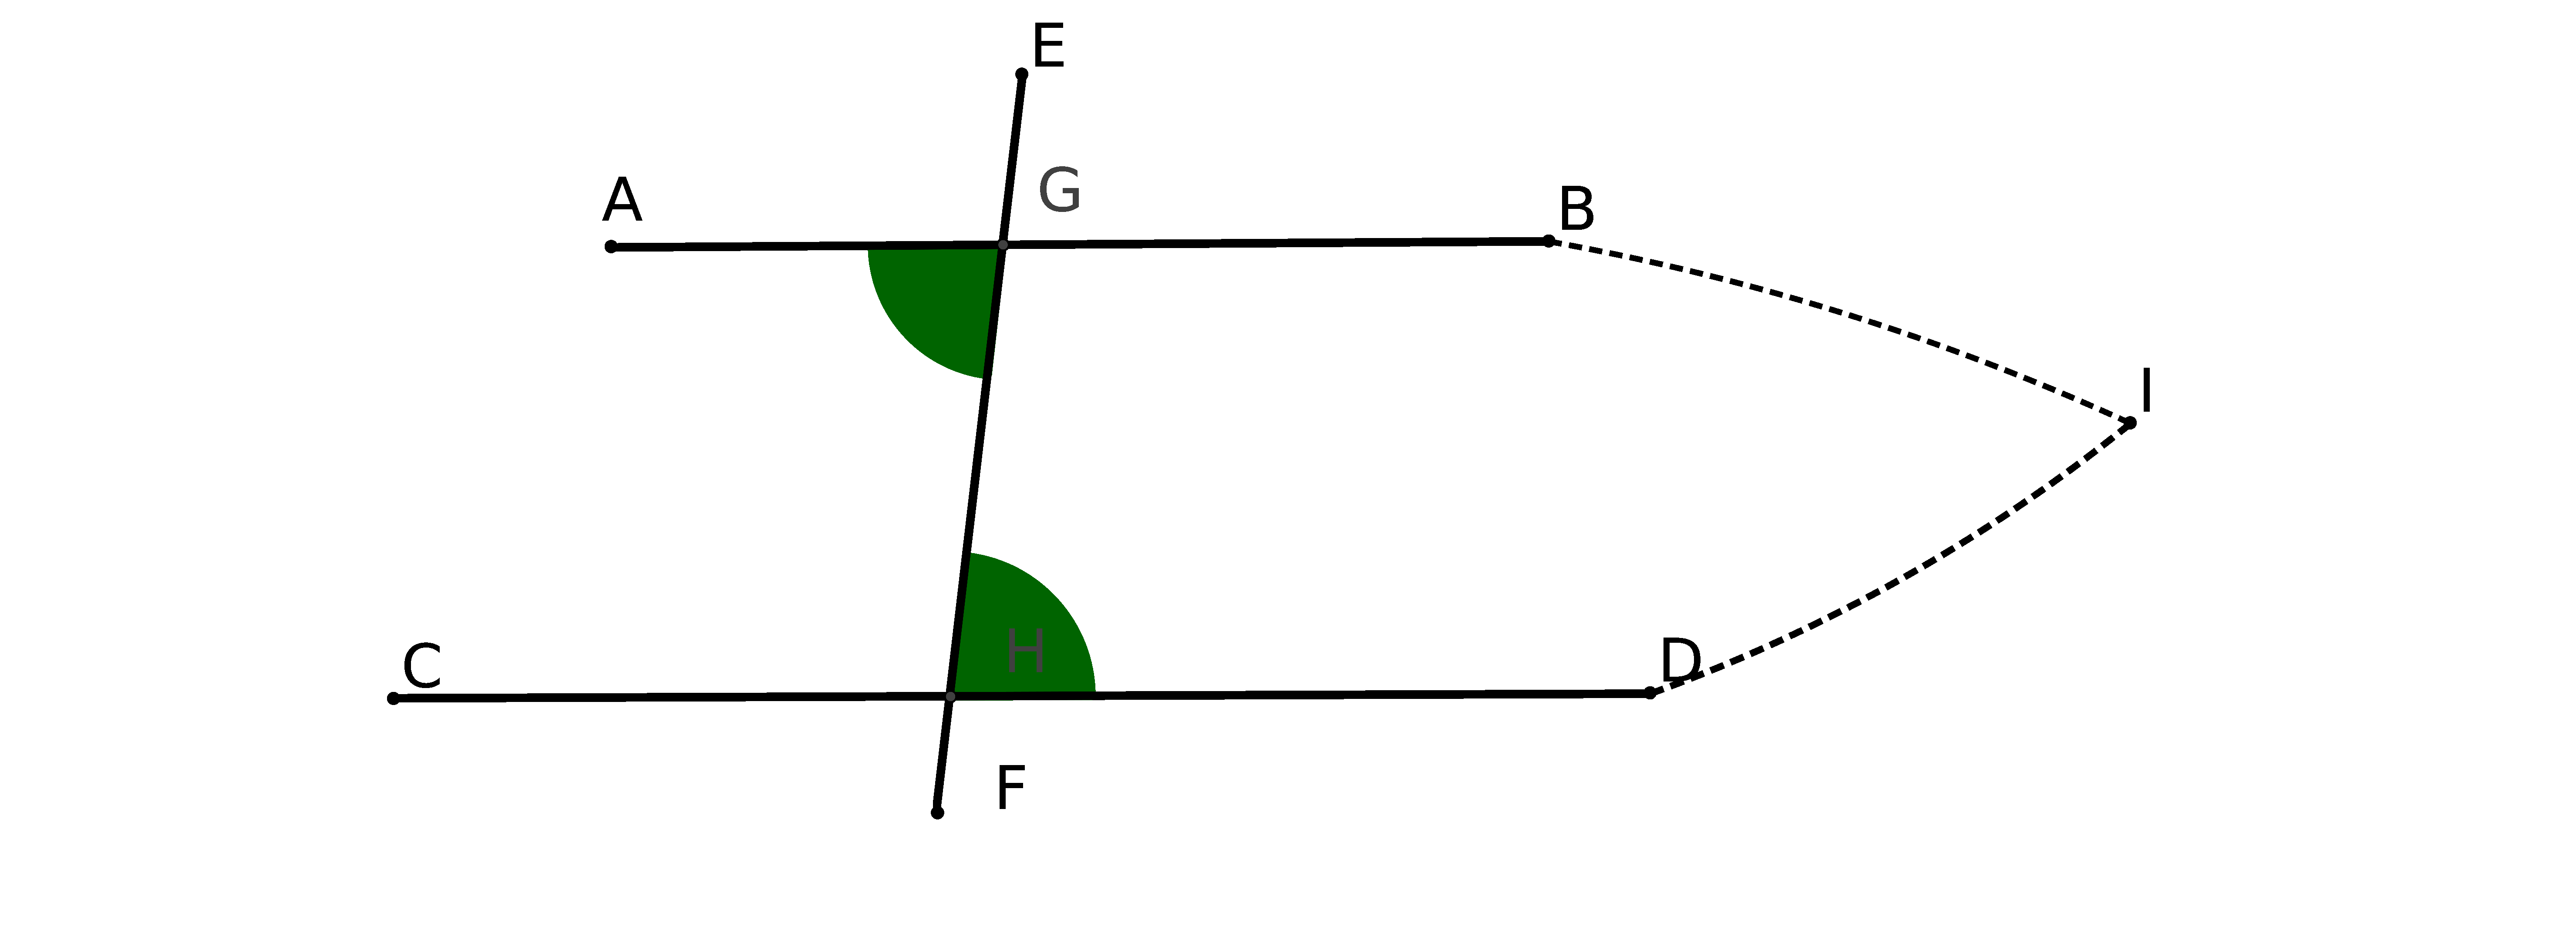
\includegraphics[scale=0.2]{figures/th27.eps} \\
  
  \textit{démonstration:} soient deux droites AB et CD coupées par une droite EF tel que  $\hat{AGF}=\hat{GFD}$.\
  
  Supposons que AB et CD se coupent en I. Alors dans le triangle IGF, l'angle extérieur $\hat{AGF}$  est égal à l'angle opposé $\hat{GFD}$. Contradiction avec th16.1. Donc AB et CD sont parallèles.\\
  
  \textit{Commentaire:} C'est la première fois que l'on rencontre des droites parallèles et leur existence dépend du théorème 16.1.\\
  
  
  
   
  
  
    
  
  
 
  \newpage \textbf{théorème 28: si une droite tombant sur deux droites fait extérieurement un angle égal à l'angle intérieur et opposé ou fait deux angles égaux à deux droits, ceux intérieurement sur le même côté, alors les deux droites sont parallèles.}\\
  
  
 
 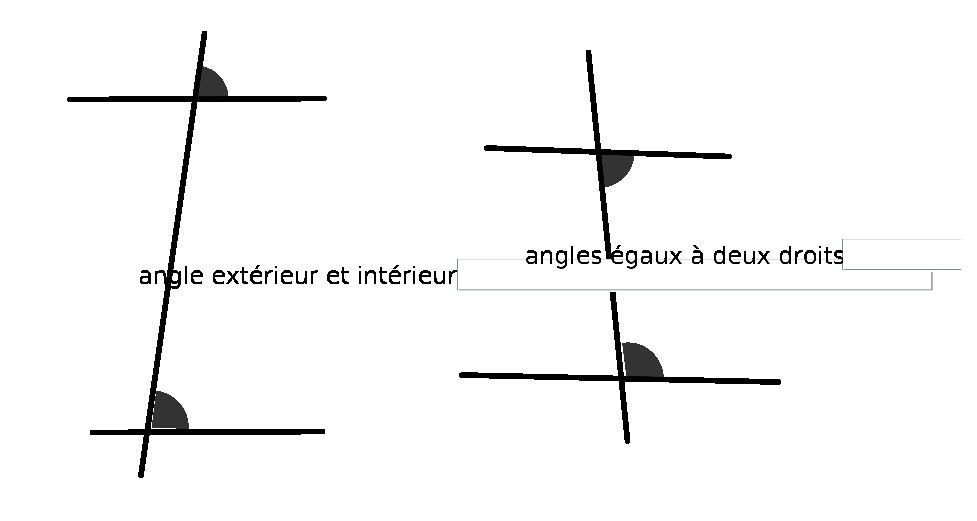
\includegraphics[scale=0.7]{figures/LIVRE1&28.eps} \\
 
 
 
  \subsection{Livre 1: Théorèmes faisant intervenir P5.}
 
  \textbf{théorème 29: la droite, tombant sur deux droites parallèles, fait extérieurement un angle égal à l'angle intérieur et opposé et fait deux angles égaux à deux droits, ceux intérieurement sur le même côté.}\\
  
  \textit{Démonstration:} Soit la droite EF coupant les droites AB et CD en G et H.
 
  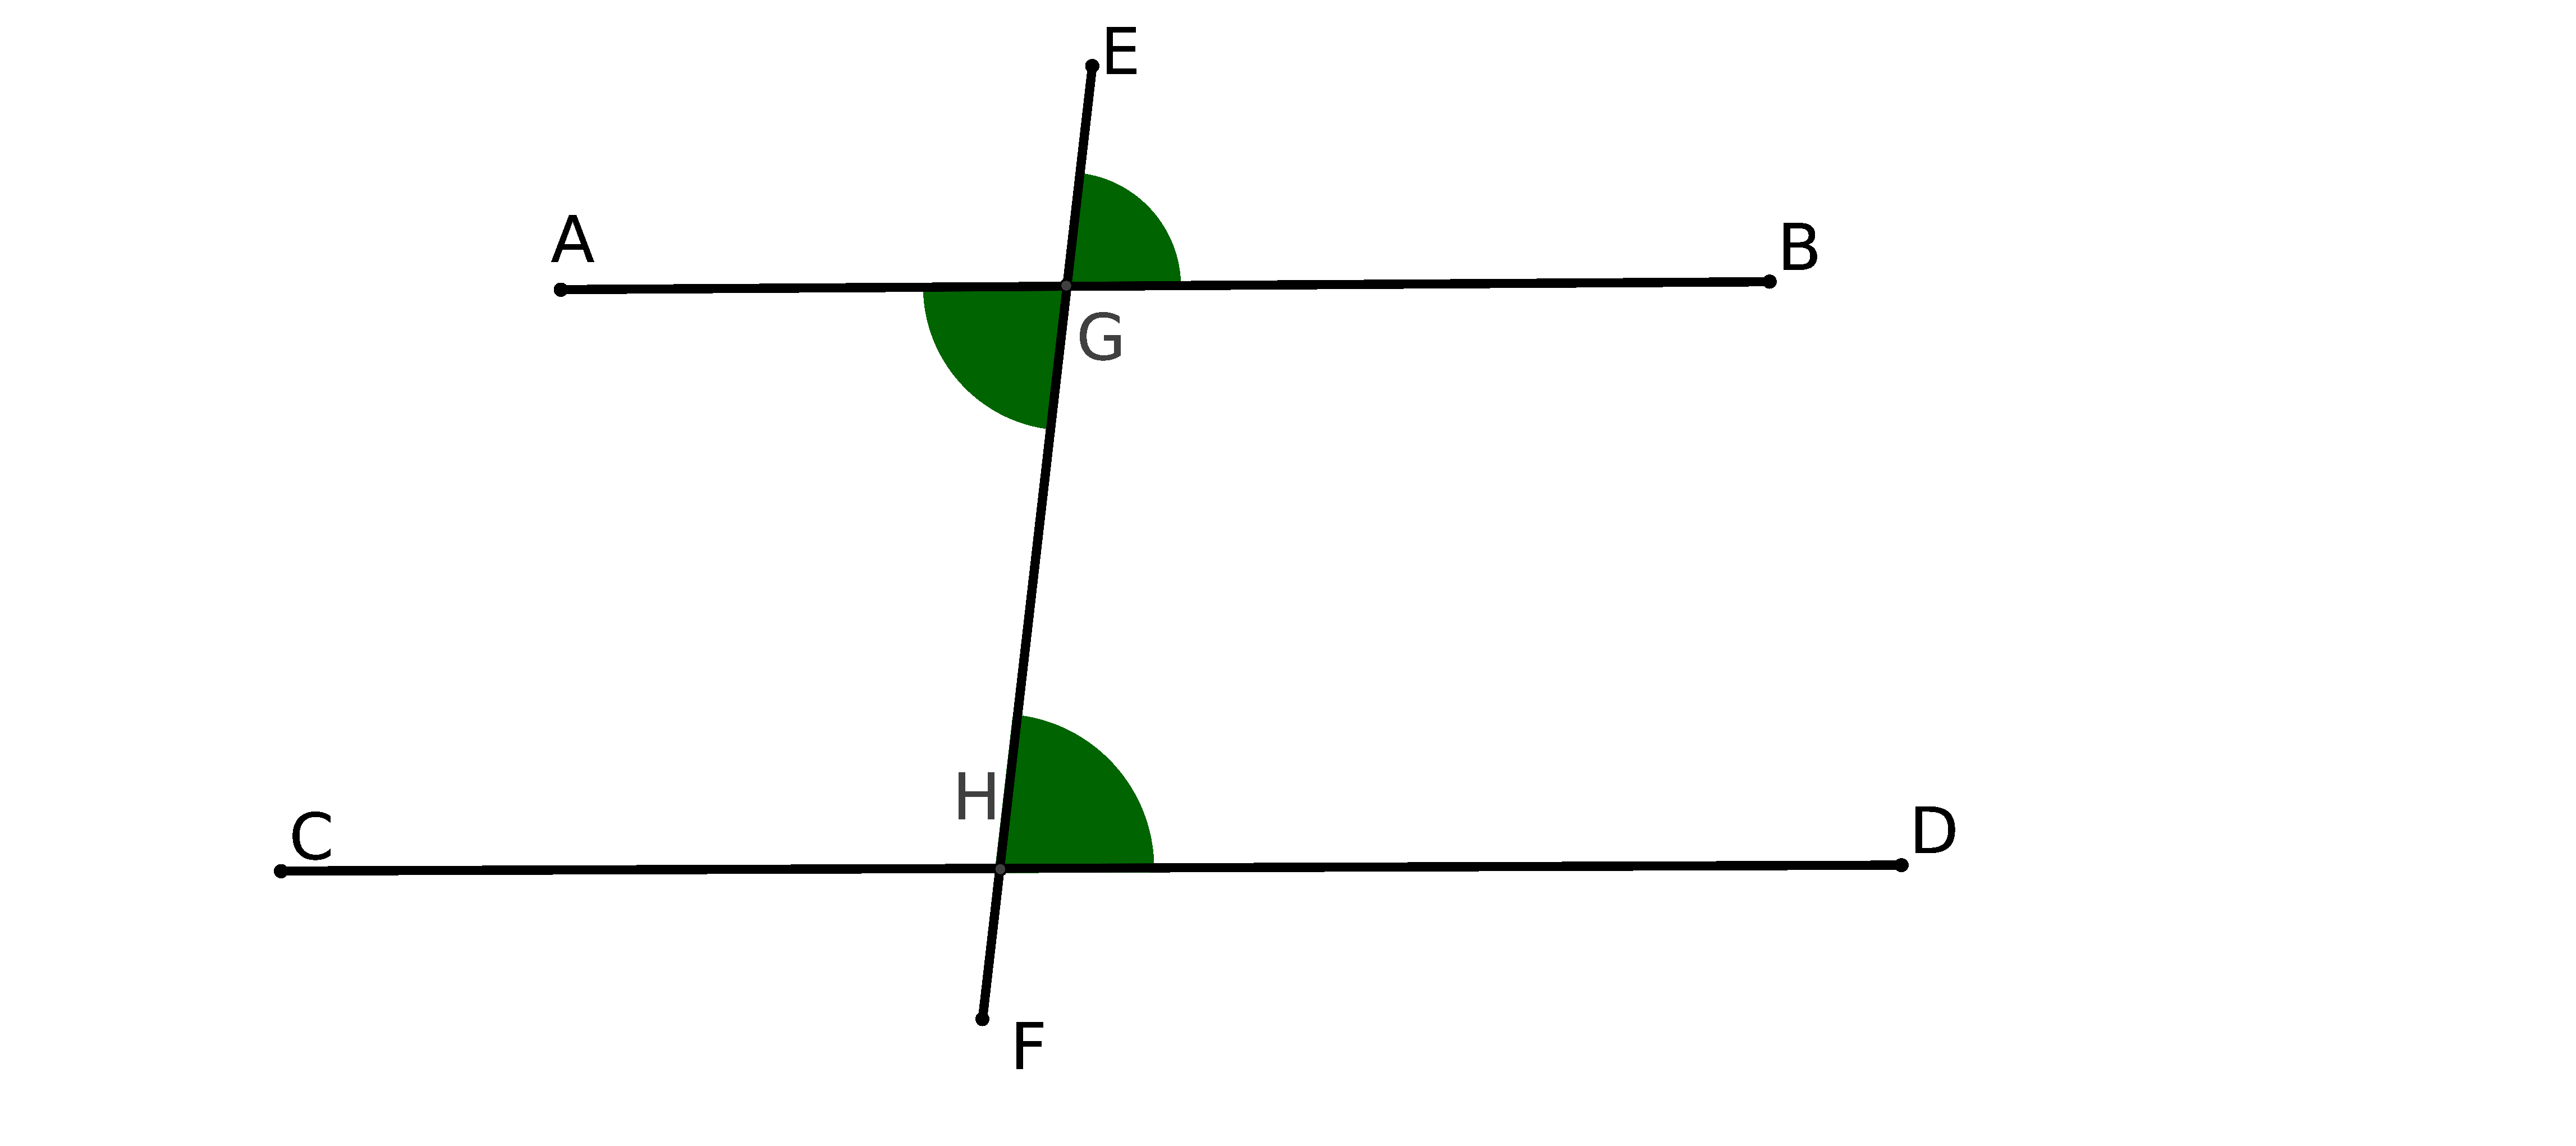
\includegraphics[scale=0.2]{figures/th29.eps} \\
  
  
 Supposons que $\hat{AGH}>\hat{GHD}$. Alors  $\hat{AGH}+\hat{BGH}>\hat{GHD}+\hat{BGH}$ (A2).\
 
 Donc $\hat{GHD}+\hat{BGH}<$2 droits.\
 
 Donc D'après P5, AB et CD sont sécantes. Contradiction.\
 
 Il est facile de démontrer ensuite que  $\hat{BGH}+\hat{GHD}=$2 droits.\\
 
 \textbf{Théorème 30: les droites parallèles à une même droite sont parallèles entre elles.}\\
 
 \textit{ Démonstration:} 
1. On prend deux droites AB et CD parallèles à une même droite EF.\\ 

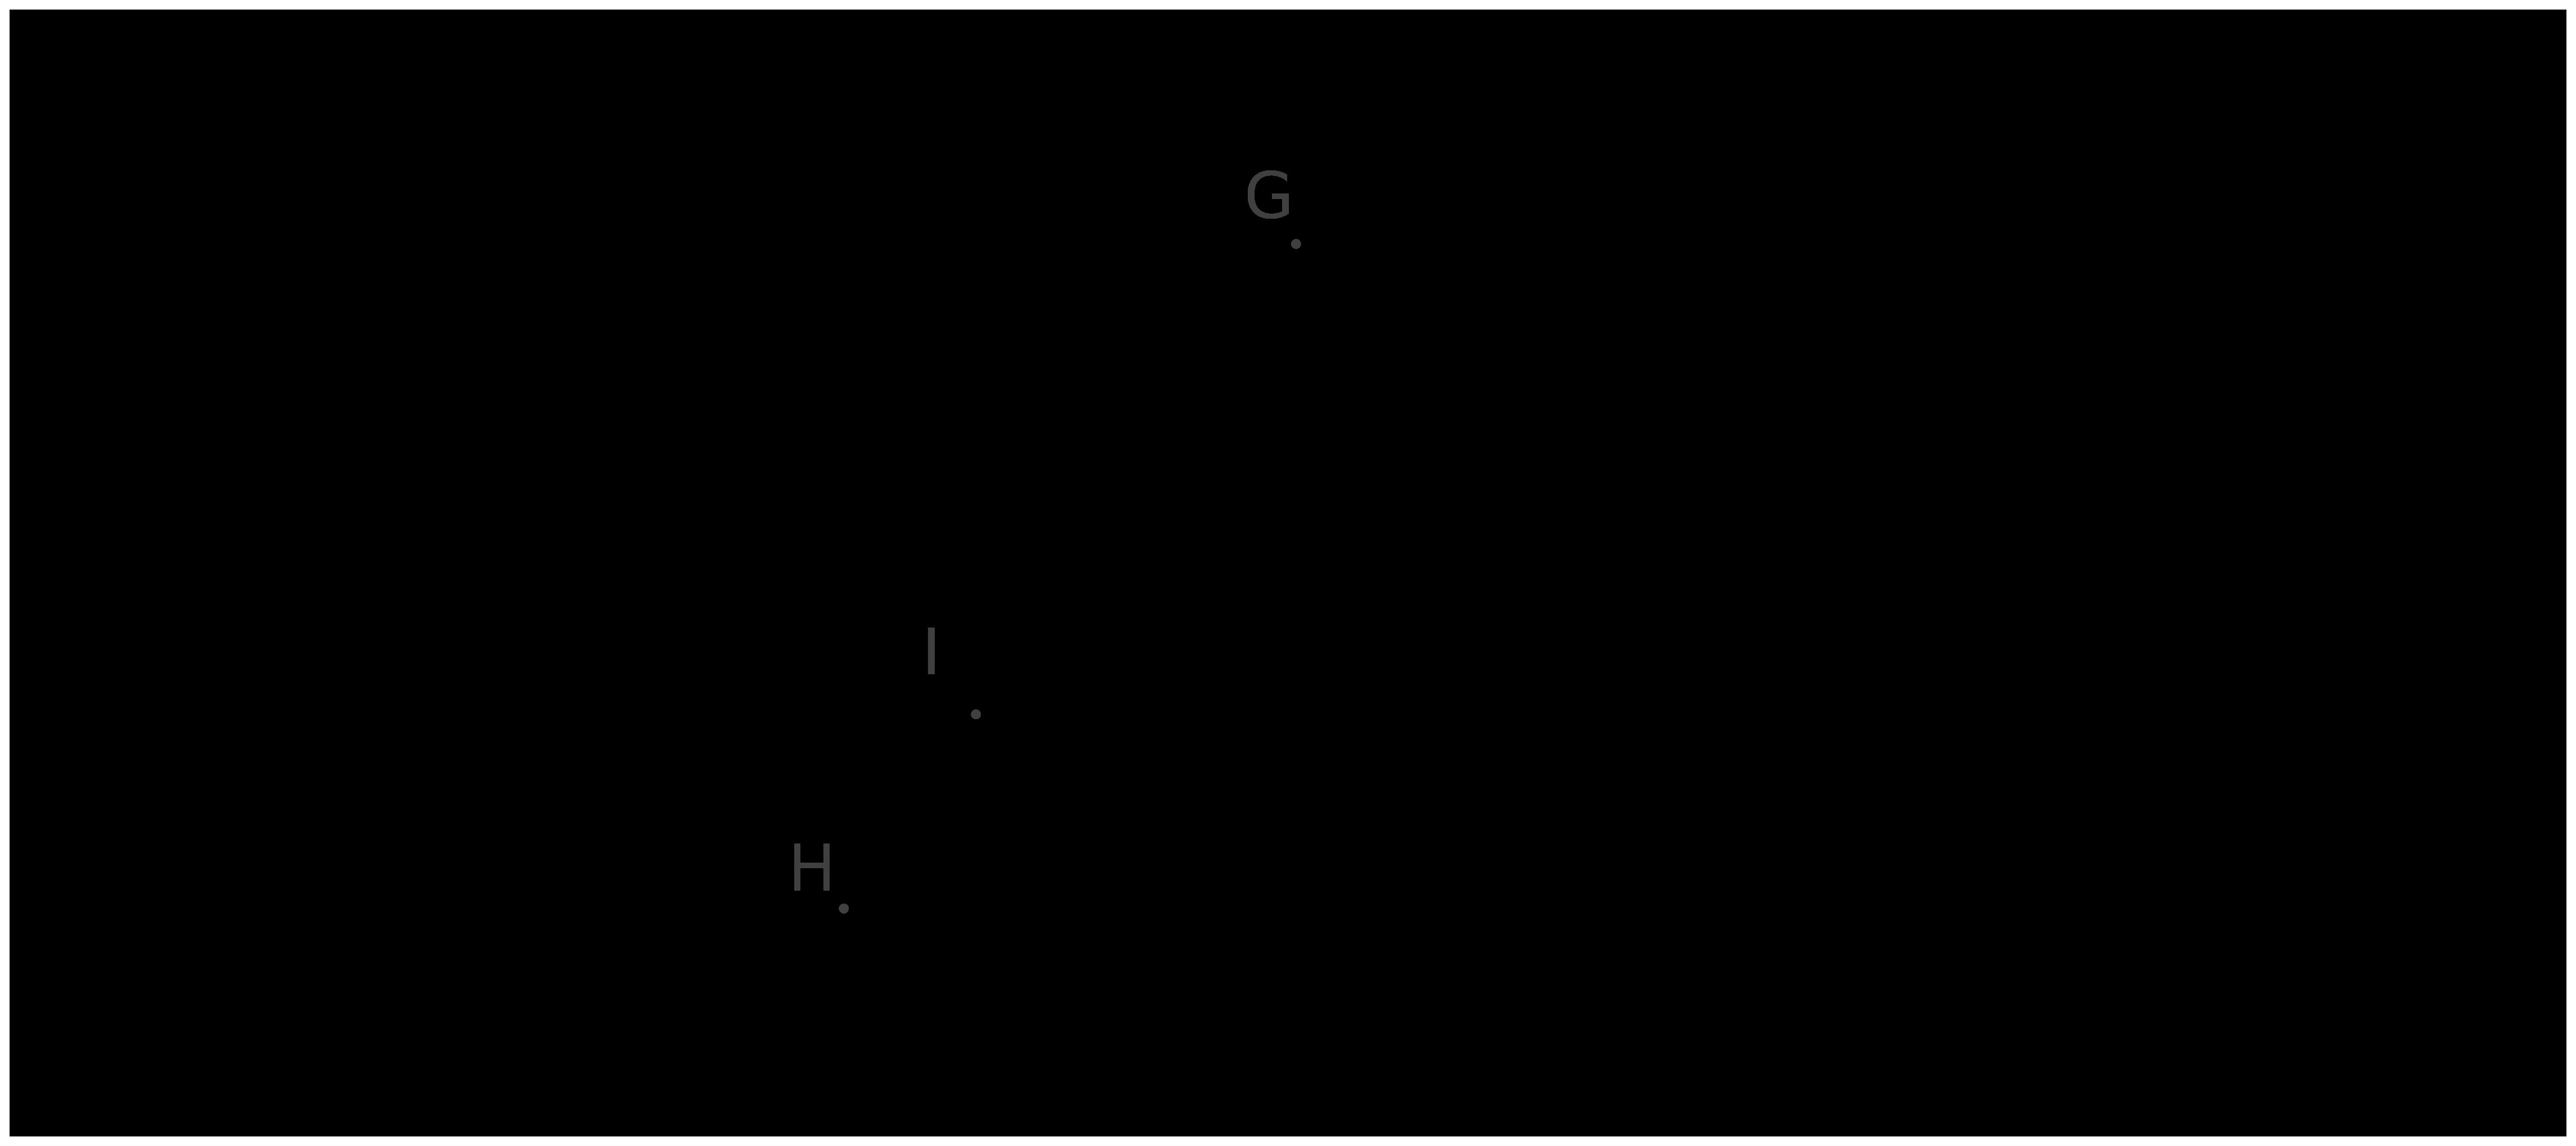
\includegraphics[scale=0.2]{figures/th30.eps}\\


2. Soit une droite GI coupant les droites EF et CD. Alors elle coupe aussi AB en H. \textit{Euclide ne le démontre pas. GI pourrait-être parallèle à AB. L'unicité d'une parallèle à une droite donnée et passant par un point donné n'est pas encore établie! Une fois de plus, on "voit" que...}.\





 3. AB et EF sont parallèles donc (Th 29.1) $\hat{EGH}= \hat{BHG}$. De même CD et EF d'où  $\hat{EGI}= \hat{DIG}$.\\
 4. Donc $\hat{EGH}= \hat{EGI}$ (th29.1) donc $\hat{BHG}= \hat{DIG}$. Donc (Th 28.1) AB et CD sont parallèles.\\
 
 
 \textit{commentaire:} on applique th28.1 et th29.1.\\
 
  \textbf{Théorème 31: construire une parallèle à une droite donnée et passant par un point donné.}\\
 
 
 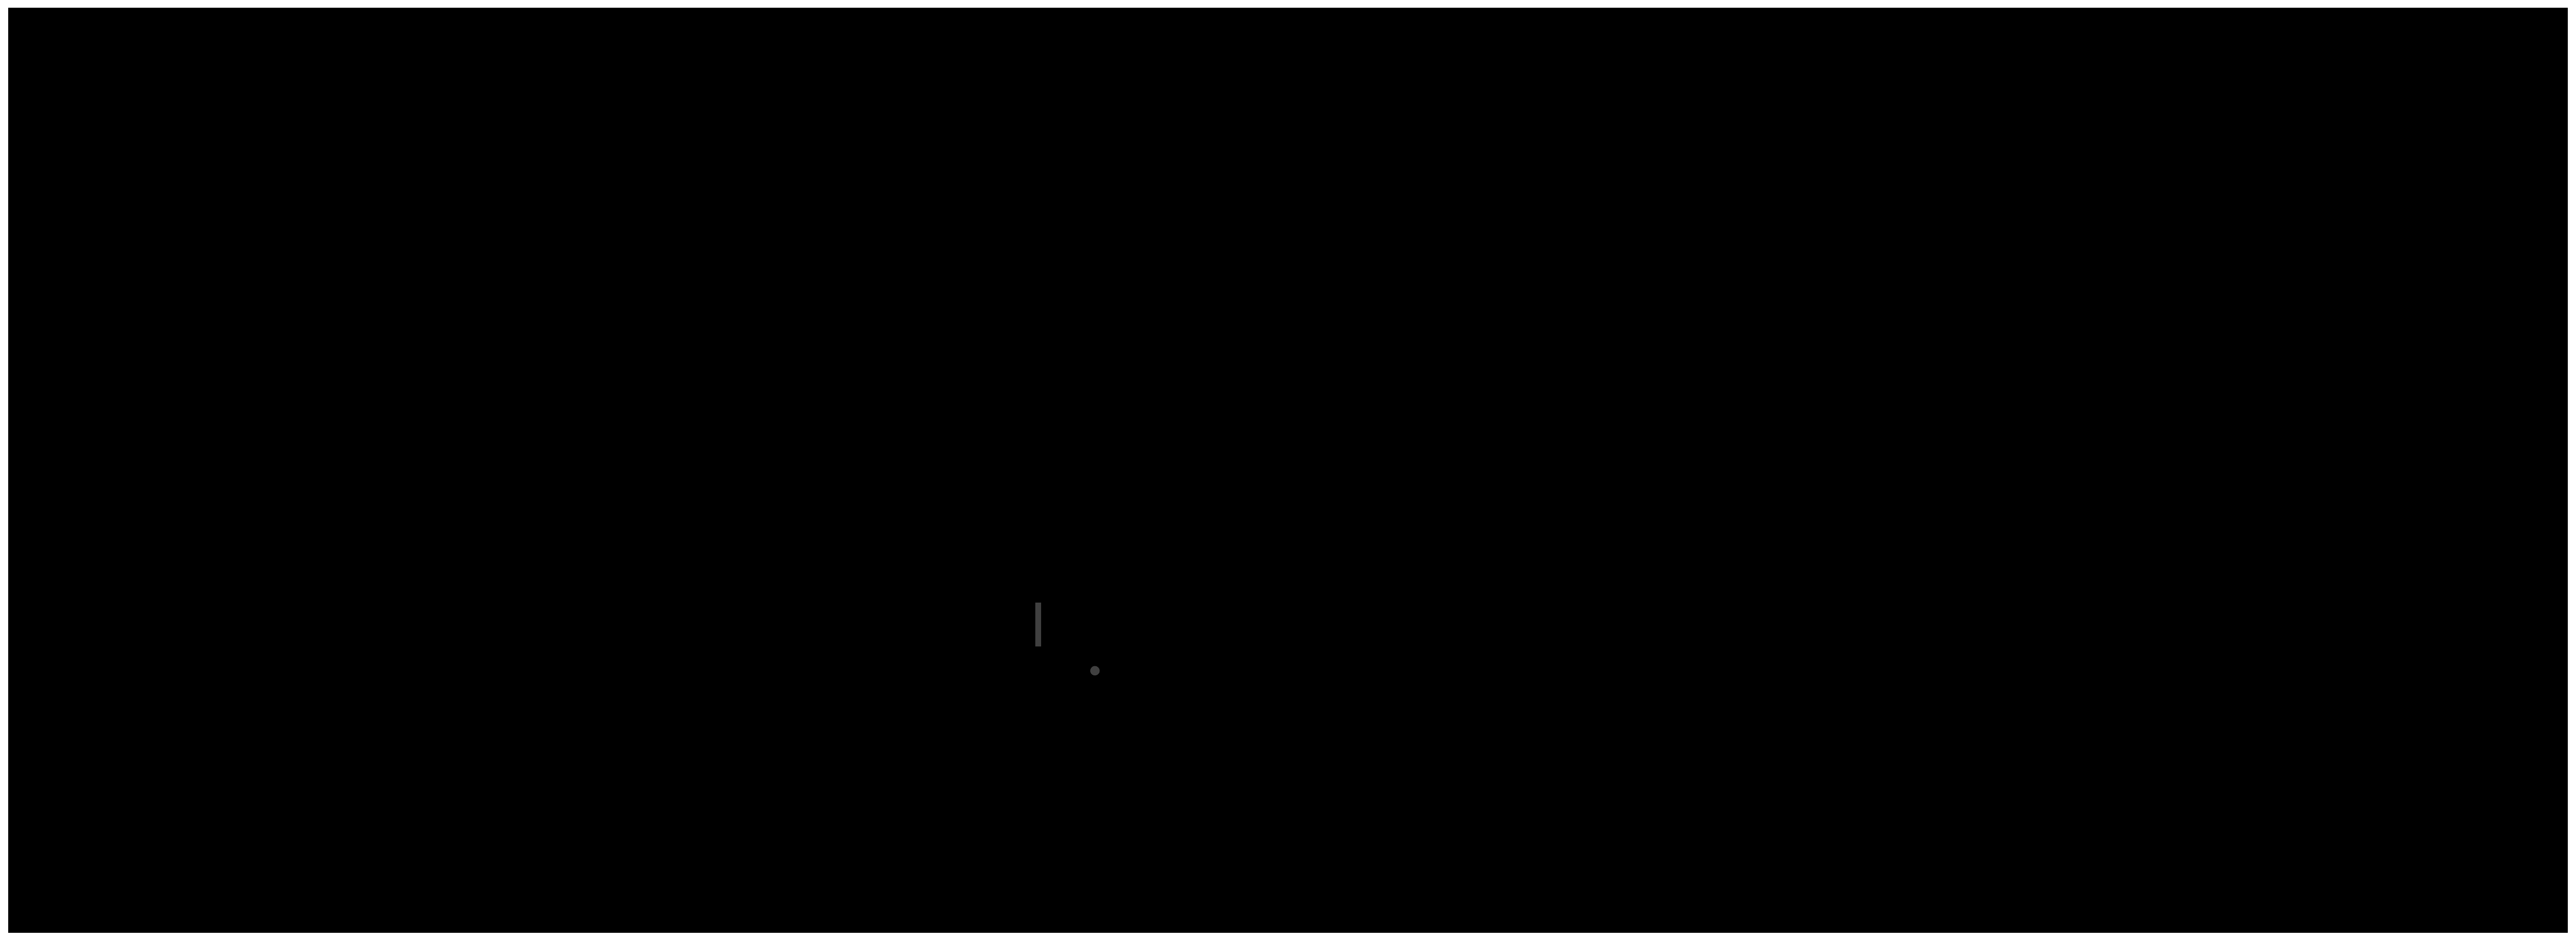
\includegraphics[scale=0.2]{figures/th31.eps} \\ 
 
 \textit{Démonstration:} soit CD une droite et soit A un point. Soit B un point de CD. On construit l'angle $\hat{EAB}$ égal à l'angle $\hat{ABD}$ (th23.1). On prolonge EA en F. Alors EF et CD sont parallèles (th27.1).\
 
 \textit{Commentaire:} il n'existe qu'une parallèle, sinon cela contredirait th29.1\\
 
 \textbf{Théorème 32: un des côtés de tout triangle étant prolongé, l'angle extérieur est égal aux deux angles intérieurs et opposés. Et la somme des trois angles intérieurs est égale à deux droits.}\\
 
 
 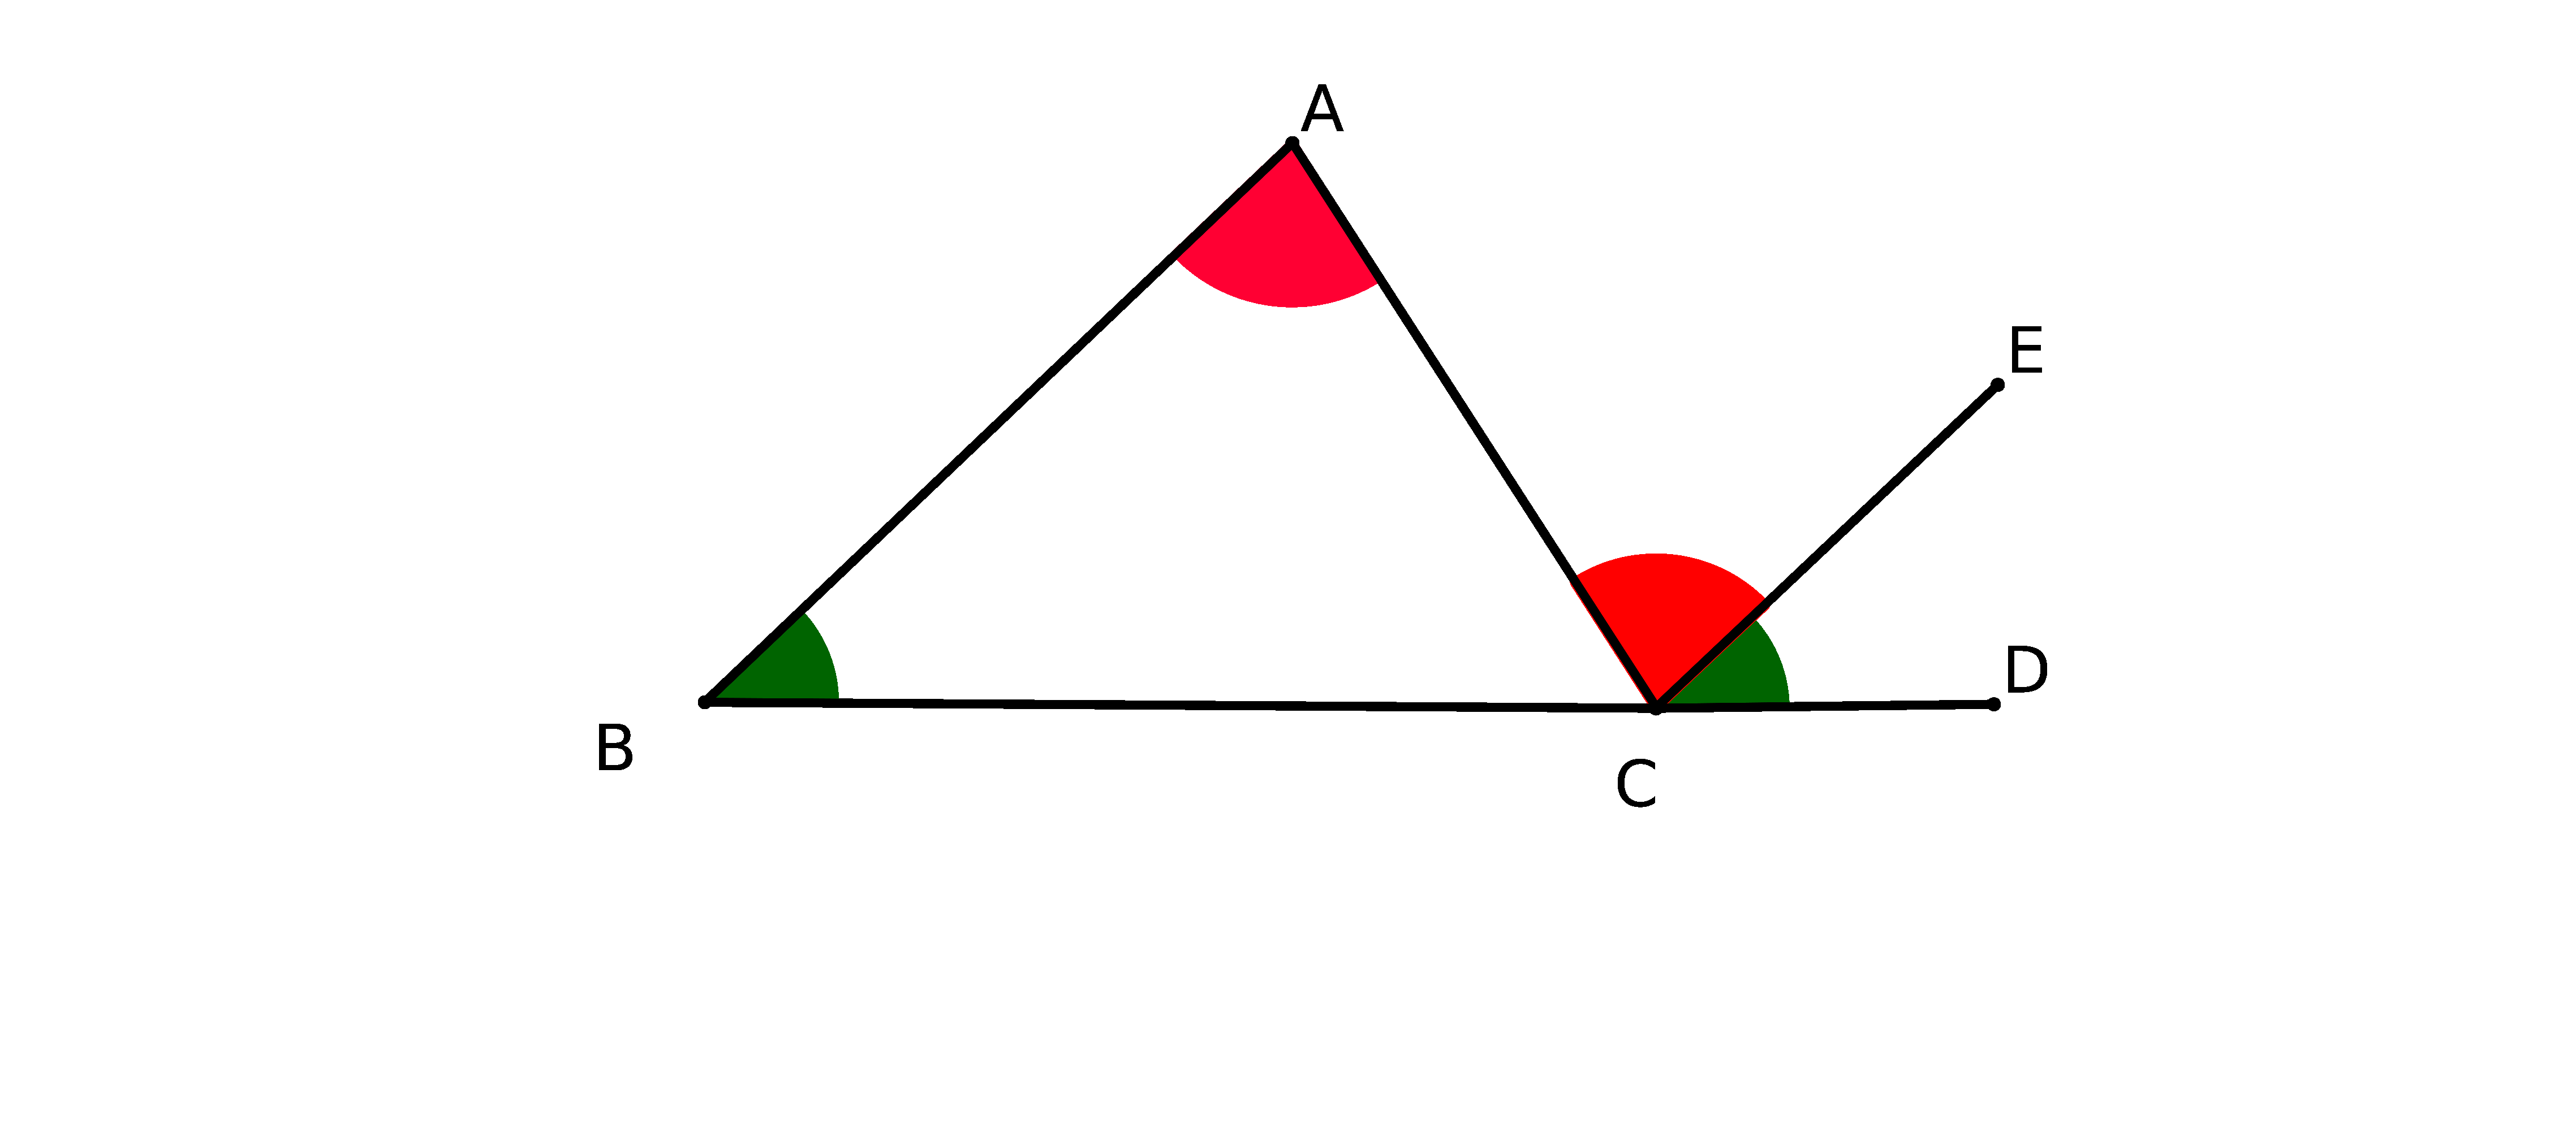
\includegraphics[scale=0.2]{figures/th32.eps} \\ 
 
 \textit{Démonstration:} On prolonge BC en D. Puis on trace la parallèle à AB passant par C (th 31.1).\
 
 On a alors: $\hat{ABC}=\hat{ECD}$ et  $\hat{BAC}=\hat{ECA}$ (th 29.1). D'où le résultat.\\
 
 \textbf{Théorème 34: les diagonales et les côtés opposés d'un parallélogramme sont égaux et leurs diagonales se coupent en leur milieu.}\\
 
 
  
 Les autres théorèmes du livre 1 nous intéressant moins, nous ne les citerons pas. Par contre la définition 1 et le théorème 18 du livre 6 nous intéressent.\\
 
 
 
  \textit{définition 1:} des figures rectilignes \textbf{semblables} sont celles qui ont les angles égaux deux à deux et les côtés, qui entourent les angles égaux, proportionnels.\\
 
 \textbf{théorème 18: sur une droite donnée construire un quadrilatère semblable à un quadrilatère donné.}\
 
 \textit{Remarque:} ce théorème s'applique bien entendu pour un triangle et nécessite P5. \\
  
 
 
 
 
 
 


 
  
  
 
     



 
 

 


 
 
 
 

   
  
 \newpage  Donnons un exemple de géométrie où P5 n'est pas vérifié et où il n'existe pas forcément de triangles semblables.
  
  
  
  
  
  
  
 \chapter{Géométrie sur une sphère}
  
 \section{Introduction:}
\par
   Soit une sphère de rayon R et de centre O. si on prend deux points de cette cette sphère, il passe un cercle de centre O de rayon R (  appelé géodésique  ou grand cercle).\\
   
    Chaque grand cercle est déterminé  par deux quelconques de ses points.\\
    
     On peut démontrer que, si on se munit de la distance euclidienne dans l'espace, la distance la plus courte entre deux points A et B de la sphère est la longueur du plus petit arc du grand cercle passant par A et B.  On peut s'en rendre compte facilement en coupant la sphère suivant un grand cercle joignant A et B et de voir que tout autre chemin de A à B est plus grand.\\
     
     Démontrons ce résultat:\
     
     \textit{  Faisons un rappel sur les coordonnées sphériques: soit un repère orthonormal $(O; \vec{OA},\vec{OB},\vec{OC})$.\
  Alors un point M aura pour coordonnées sphériques:.} \
  $$(r,\theta,\phi)$$
  
  \textit{et pour coordonnées cartésiennes: (on pose }$r=OM$),\\
 
  $x=r\sin \theta\cos \phi$,
  $y=r\sin \theta\sin \phi$,
  $z=r\cos \theta$ 
  
 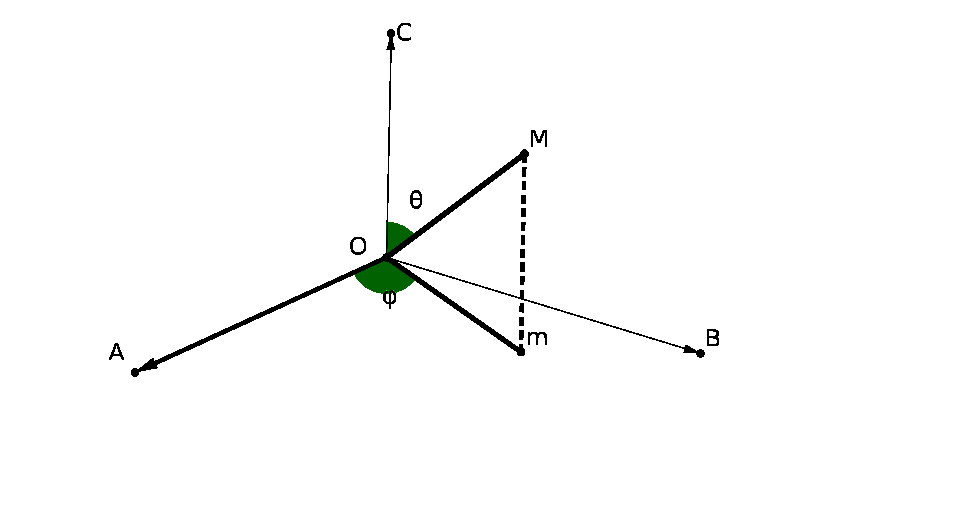
\includegraphics[scale=0.8]{figures/coordonneespheriques.eps} 
  
    \textit{Donnons nous deux points A et B de la sphère et cherchons le plus court chemin ( toujours de classe C1)les reliant.\
    Sans perdre de généralité on peut supposer que A et B ont pour coordonnées sphériques:}\
    
    $A(r,0,0)$ et $B(r,\theta_{1},0)$ .\
    
   \textit{ Alors un chemin AB sur la sphère aura pour représentation paramétrique:}\
    
    $f(t)$=$(r\cos(\phi(t))\sin (\theta(t)),r\sin(\phi)(t))\sin (\theta(t)),r\cos(\theta(t)), t\in[0,1]
$\\
\textit{avec $f(0)=A$ et $f(1)=B$}. \\

\textit{les fonctions $\theta$ et $\phi$ étant dérivables et de dérivées continues sur [0; 1] telles que:$\phi(0)=\phi(1)=0,\theta(0)=0,\theta(1)=\theta_{1}$.}\\


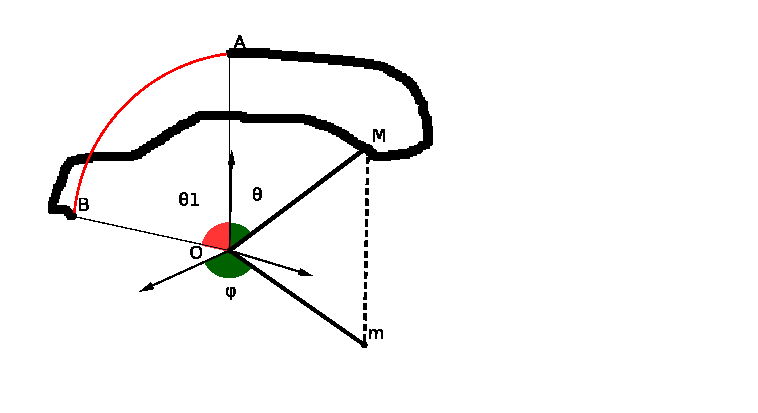
\includegraphics[scale=0.9]{figures/coordonneespheriques1.eps} 


\textit{Alors on démontre que la longueur, $l$ du chemin est égale à:}\

 $$ l=\int_{0}^{1} ||{f'}(t)|| \, \mathrm{d}t $$\
 \textit{Calculons} $||{f'}(t)||$:\\
 
 
 \textit{Si} ${f'}(t)=(x',y',z')$ alors $||{f'}(t)||=\sqrt{x'^2+y'^2+z'^2}$.\\
 
 \textit{Alors, après calcul, on trouve:}\
 
 $$||{f'}(t)||=r\sqrt{\phi'(t)^2\sin^2(t)+\theta'^2(t)}$$\\
 
 \textit{Donc:}\\
 
 $$ l=\int_{0}^{1} ||{f'}(t)|| \, \mathrm{d}t \ge r\int_{0}^{1} \sqrt{\theta'^2(t)} \, \mathrm{d}t\ge r\int_{0}^{1} \theta'(t) \, \mathrm{d}t$$\\
 
 \textit{Donc:} $l\ge r\theta_{1}$\\
 
 \textit{Et} $r\theta_{1}$ \textit{est la longueur de l'arc de cercle AB, correspondant à l'angle} $\theta_{1}$.\\
 
 




 \    
     Ainsi un arc de  grand cercle est bien le chemin le plus court d'un point à un autre, c'est donc l'équivalent sur la sphère de la ligne droite sur le plan. \\
     
     On appellera donc, sur la sphère,"droite" tout arc de grand cercle. A partir de ces"droites" on pourra construire des triangles et, plus généralement, des polygones, des cercles donc les figures que l'on peut construire dans le plan. \\
   
   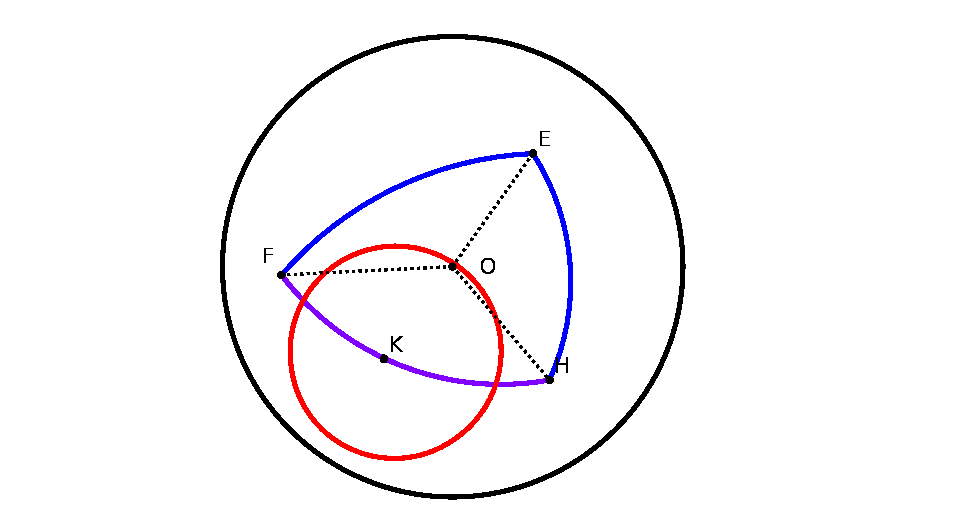
\includegraphics[scale=0.6]{figures/sphre2.eps} 
        
         Soient deux demi- grands cercles se coupant en deux points E et M. Un angle de deux droites sera l'angle défini par les tangentes à ces droites. Ces deux demi-cercles constituent un fuseau.\\

  
           
    
         
    
     
     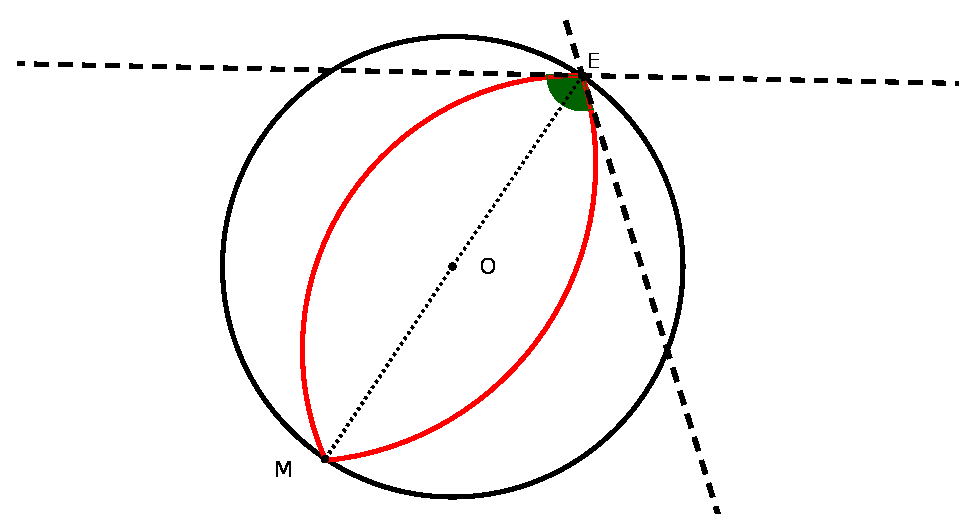
\includegraphics[scale=0.6]{figures/sphre1.eps} \\
     
 \section{Somme des angles:}\
 
      
     Dans ce qui suit on considère une sphère de rayon 1.\\
        
     Démontrons que si un angle d'un fuseau est $\theta$ alors l'aire du fuseau est 2$\theta$. En effet la sphère a pour surface 4$\pi$ et correspond à un angle de 2$\pi$. D'où le résultat.\\
     
     Nous avons donc défini les notions de droites et d'angle sur la sphère.\
    
     
     Notre géométrie sur la sphère présente trois inconvénients: tout d'abord,si deux points sont diamétralement opposés, il y a une infinité de grands cercles (donc de droites) passant par ces deux points donc deux droites formant un fuseau pourront entourer un domaine, donc le sixième postulat ne sera pas vérifié.\
     
      Ensuite un grand cercle ne peut pas se prolonger de manière continue autant que l'on veut, donc le deuxième postulat d'Euclide n'est pas non plus vérifié.\
      
       Pour éviter le premier inconvénient on appellera point toute paire de points diamétralement opposés.\
       
     Les droites seront toujours les grands cercles.\
     
     Ainsi quels sont les postulats vérifiés?  \
     
     1. Par deux points  passe une droite. (Postulat 1)\
     
     2. On  ne peut pas prolonger autant que l'on veut une droite puisqu'elle est finie. Donc le Postulat 2 n'est pas vérifié.\
     
     3. On sait tracer un cercle. (Postulat 3)\
     
     4. Tous les angles droits sont égaux. (Postulat 4)\
     
     6. Deux droites peuvent entourer un domaine. Donc le Postulat 6 n'est pas vérifié.\\
     
      \textit{Ceci a pour conséquences, en particulier, que le théorème 4 d'Euclide n'est pas vrai et qu'il n'y a pas de droites parallèles car deux grands cercles ont toujours un point commun.}\\
     
     
    Démontrons maintenant le théorème suivant: \textit{\textbf{la somme des angles d'un triangle, d'angles $\alpha$, $\beta$ et $\gamma$ et d'aire T est égale à $\pi$+T}}.\\
    
    
    cf à la figure suivante:\\
    
     On pose  EFH=$\alpha$,FHE=$\beta$, HEF=$\gamma$.\\
     
   Démontrons que\\ $EFH+FHE+HEF$=$\alpha$+$\beta$+$\gamma$+$T$. \\    
 
 Soit S' la demi-sphère contenant E et limitée par le grand cercle (FH). Alors S' a pour aire 2$\pi$.\\   
  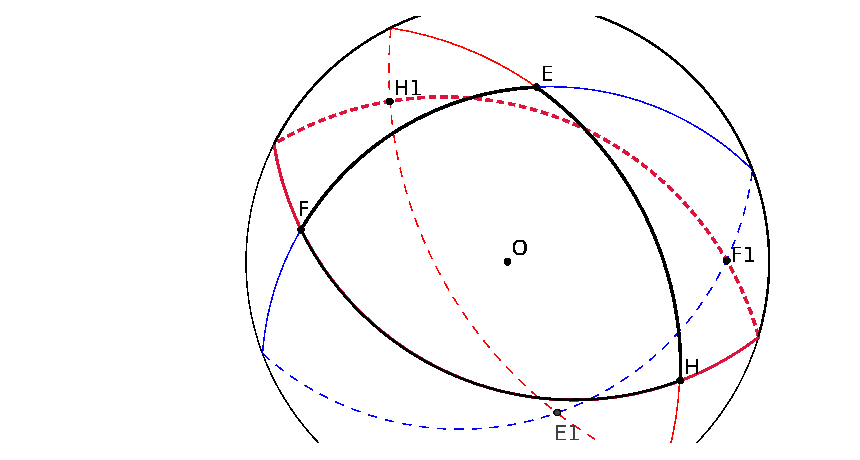
\includegraphics[scale=0.7]{figures/sphre5ter.eps} \\   
     
 


Mais S' est la réunion du fuseau de sommets F et F1 et contenant le triangle EFH  \\
et du complémentaire du triangle EFH dans le fuseau de sommets H et H1 contenant le triangle EFH  \\
et du complémentaire du  triangle E1F1H1 dans le fuseau de sommets E et E1 et contenant le triangle E1F1H1, triangle de même aire que  EFH par symétrie.\\

Donc 2$\pi$=2$\alpha$+2$\beta$-T+2$\gamma$-T.

Donc $\pi$+T=$\alpha$+$\beta$+$\gamma$.\\


Ainsi, la somme des angles d'un triangle sur une sphère est supérieure à $\pi$.\\

On peut remarquer que, aussi, que la somme des angles \textbf{dépend de l'aire du triangle}.\\


Dans la géométrie euclidienne la somme des angles est égale à 2$\pi$ et c'est une conséquence de P5! Donc si, sur la sphère, ce n'est pas vrai,  P5 serait faux sur la sphère! Or, sur la sphère, deux droites quelconques sont sécantes, donc P5 est vrai! Donc tout simplement parce que le théorème: la somme des angles dans un triangle est égale à  2$\pi$, ne dépend pas que de P5. \\

\newpage   \section{Triangles semblables:}
  
  Y a-t-il des triangles semblables sur une sphère?\\
  
  Deux triangles sont semblables s'ils ont des angles égaux 2 à 2 ou encore si leurs côtés sont proportionnels.(Définition 1 livre 6)\\
  
  Soient donc deux triangles ABC et A'B'C' non égaux. On les suppose semblables et par déplacement on peut supposer que les points A et A' sont confondus.\\
  
  
  \subsection{Que peut-on dire des angles?}
 
  
  Prenons donc deux triangles qui ont leurs angles égaux deux à deux.\
  
  Posons $\hat{A}$=$\hat{A'}$=$\alpha$ , $\hat{B}$=$\hat{B'}$=$\beta$ et $\hat{C}$=$\hat{C'}$=$\gamma$.\\
    
  Si les deux triangles ont les mêmes angles alors la somme de leurs angles est la même donc $\pi+T=\pi+T'$, T et T' étant leurs aires respectives. Donc $T=T'$. Ce qui n'est pas possible.\
 
 Donc s'il existe des triangles semblables cela ne peut pas être par rapport à leurs angles. \\\
 
  
   On peut supposer que B' est sur AB, C' sur AC. On aura donc une figure du type:
  
  
  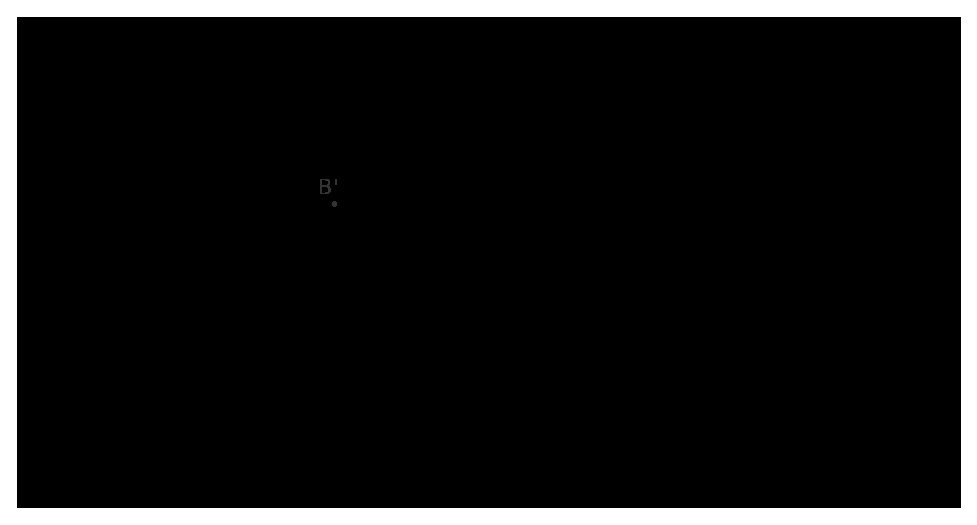
\includegraphics[scale=0.7]{figures/sphre6.eps}\
   
  
  \newpage   \subsection{Que peut-on dire des côtés?}
  
 Prenons deux triangles, ABC et A'B'C', qui ont leurs côtés proportionnels.\
 
  Par déplacement on peut supposer que B' est sur AB. Rappelons que, la sphère étant de rayon 1, la longueur de l'arc AB est égale à $\hat{AOB}=c$ en radians. Posons dans la figure suivante:\\
  
  
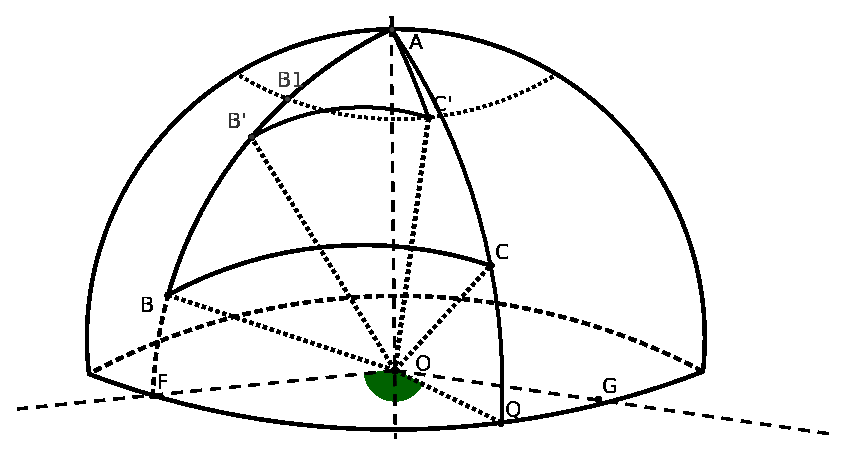
\includegraphics[scale=0.7]{figures/demi-sphere2bis.eps} \\
 
  $\hat{AOB}=c$ et $\hat{AOB'}=c'$,
  $\hat{AOC}=b$ et $\hat{AOC'}=b'$, 
  $\hat{COB}=a$ et $\hat{C'OB'}=a'$ et 
  $\hat{FOQ}=\alpha$ \ 
  
  Supposons les côtés AB' et AC' proportionnels aux cotés AB et AC, c'est à dire supposons qu'il existe un réel $k,k\in ]0; 1[$ tel que $c'=kc$ et $b'=kb$. \
  
  Les côtés BC et B'C' sont-ils dans le même rapport, comme cela serait le cas en géométrie euclidienne? C'est à dire a-t-on $a'=ka$?\
  
  
  Traitons l'exemple suivant: \ $c=\frac{\pi}{3}$,  $b=\frac{\pi}{2}$ et $k=\frac{1}{2}$. On a donc $c^{'}=\frac{\pi}{6}$ et $b^{'}=\frac{\pi}{4}$ et on a la figure suivante:\\
  

 
 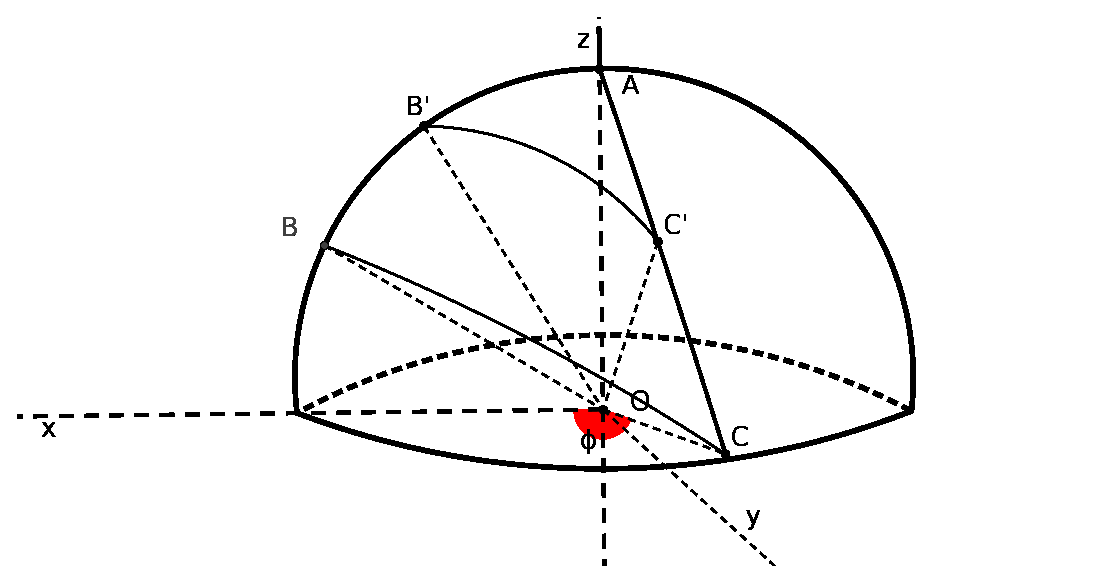
\includegraphics[scale=0.7]{figures/demi-sphre2ter.eps} \\
 
 Les coordonnées de B, B', C et C' sont \
 
 B($\dfrac{\sqrt{3}}{2}$, 0, $\dfrac{1}{2}$)\
 
 B'($\dfrac{1}{2}$, 0, $\dfrac{\sqrt{3}}{2}$)\
 
 C ( cos($\Phi$), sin($\Phi$),0) et \
 
 C'($\dfrac{\sqrt{2}}{2}$cos($\Phi$), $\dfrac{\sqrt{2}}{2}$sin($\Phi$),$\dfrac{\sqrt{2}}{2}$).\\
 
 On $\vec{OB}.\vec{OC}=cos(a)=\dfrac{\sqrt{3}}{2}cos(\Phi)$ et\
 
  $\vec{OB^{'}}.\vec{OC^{'}}=cos(a^{'})=\dfrac{\sqrt{2}}{4}cos(\Phi)+\dfrac{\sqrt{6}}{4}$.\\
  
  Si les deux triangles ont leurs côtés proportionnels on devrait avoir $a^{'}=\frac{a}{2}$ ou encore, puisque $cos(a)=2cos^{2}(\frac{a}{2})-1$,\
  
 $\dfrac{\sqrt{3}}{2}cos(\Phi)=2(\dfrac{\sqrt{2}}{4}cos(\Phi)+\dfrac{\sqrt{6}}{4})^{2}-1$. \
 
 Après calculs on obtient: cos($\Phi$)=1 ou cos($\Phi$)=-1. Mais dans ces deux cas le triangle ABC n'existe pas donc, pour tout $\Phi\neq 0$ modulo $\pi$, $a^{'}\neq\frac{a}{2}$.\
 
 Ainsi aucun triangle n'est semblable au triangle ABC dans le rapport $\frac{1}{2}$.\\
 
  
 La similitude des triangles ne peut-être définie dans la géométrie de la sphère
  
  
  
  
  
  On voit donc une fois de plus que l'on n'est plus dans le cadre de la géométrie euclidienne.
  
 \chapter{Posidonius:}\
 
 Rappelons que Posidonius, pour démontrer P5, changeait la définition des droites parallèles en affirmant que deux droites sont parallèles si et seulement si elles sont équidistantes.\\
 

 
 Tout d'abord comment définir cette notion d'équidistance avec les éléments d'Euclide? \\
 
a) \textit{Définissons d'abord la notion de distance d'un point à une droite}\

Soit M un point et AB une droite.  \

Le Th12.1 nous permet d'affirmer l'existence de la perpendiculaire à AB passant par M. Soit MP cette perpendiculaire.\\

 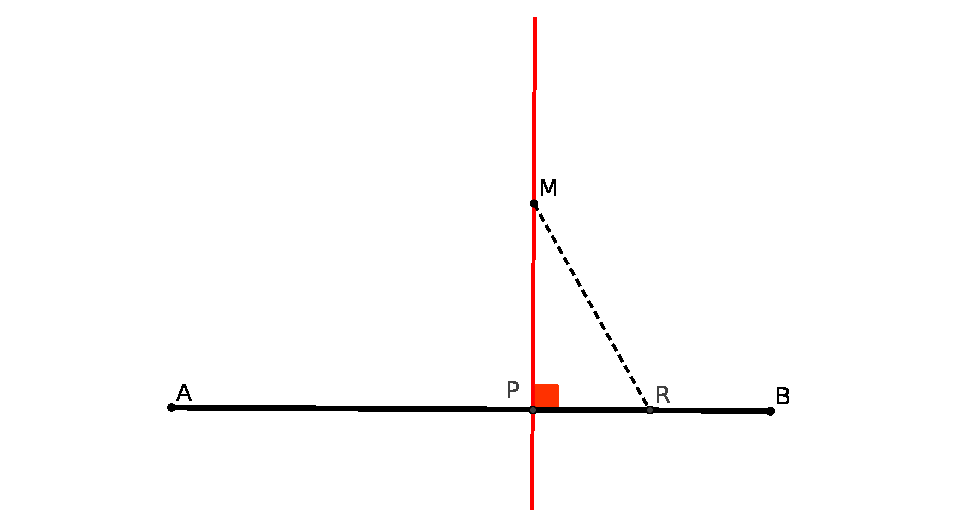
\includegraphics[scale=0.6]{figures/posi6.eps} \\
 
Soit R un point de AB distinct de P. D'après Th16.1 l'angle MPA est plus grand que chacun des angles intérieurs et opposés du triangle MPR.\

Ainsi, d'après Th18.1, MR est plus grand que MP\\

On appellera distance de M à AB la droite MP.\\

  b)\textit{Définition de Posidonius}\\
 
 
 
 Soient deux droites AB et CD. AB est parallèle à AB lorsque, pour tous points, M et N, de AB.  les perpendiculaires, MP et NQ à CD sont égales. \\
 
 c) \textit{Supposons que deux droites AB et CD sont parallèles au sens de Posidonius. Peut-on en déduire P5?}\\
 
 Soient donc deux  points, M et N, de AB et  les perpendiculaires, MP et NQ à AB.\\
 
   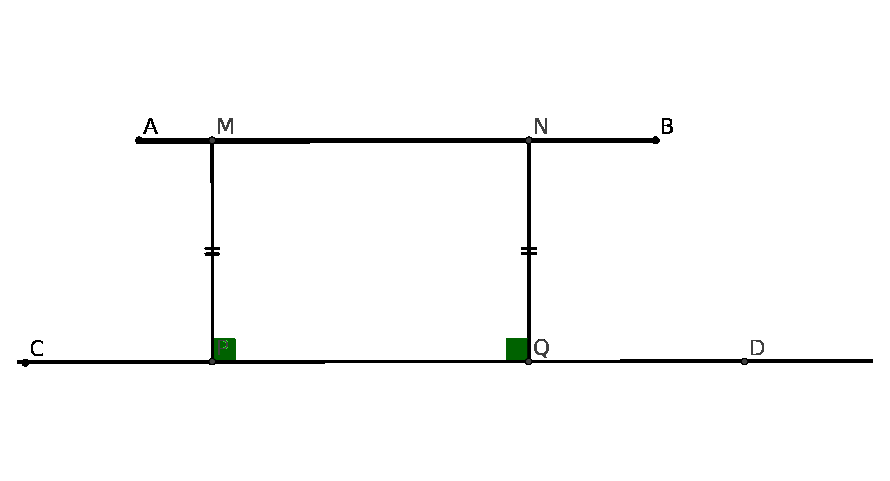
\includegraphics[scale=0.6]{figures/posi1.eps} \\
 
 Ainsi on obtient un quadrilatère MNQP qui a deux angles droits et deux côtés égaux. C'est le rectangle de Saccheri. On ignore si les deux autres angles sont droits.\\
On va voir avec Saccheri que l'on ne peut déduire P5 que si les quatre angles sont droits. Mais alors, si les quatre angles sont droits, cela signifie que dans la définition de l'équidistance, on doit admettre que des droites parallèles sont des droites qui admettent des perpendiculaires communes et que toutes ces perpendiculaires communes sont égales.\

Or dans les Eléments d'Euclide, ce résultat est une conséquence de P5. \\

On voit donc, qu'avec sa définition, Posidonius ne peut pas démontrer P5. Soit elle est insuffisante soit elle contient déjà P5. \\

d) Enfin, si deux droites sont parallèles au sens d'Euclide, elles sont équidistantes si on admet P5. C'est une conséquence du Th34.1.\\  
 
  
\chapter{Al Jahwari:}\

Al Jawhari remplace P5 par l'énoncé suivant, que l'on nommera PJ:\

 \textbf{par un point quelconque situé à l'intérieur d'un angle, il est possible de tracer une ligne coupant ses deux côtés.  Puis il se propose de démontrer P5. Mais on peut prouver que les deux énoncés sont équivalents.} \
 
 Il pense que son énoncé est indépendant de P5 et qu'il ne dépend que de des postulats autres que P5. Ainsi, pour lui, il fait partie de ce que l'on appelle la géométrie neutre. Nous allons voir que c'est faux!\\
 
 

\section{Prouvons d'abord que si PJ est vrai alors P5 est vrai.}


Soient deux droites AT et ME coupant la droite MT telles que A et E sont du même côté de MT et tels que la somme des angles qu'elles font avec MT est inférieure à deux droits.\\

Rappelons P8 postulat que nous avons rajouté et qui postule que la droite joignant deux points, situés de part et d'autre d'une même droite, coupe cette droite.\\

Si M et E ne sont pas du même côté de AT alors ME coupe AT et c'est fini. \\

Supposons que M et E sont du même côté de AT. \\


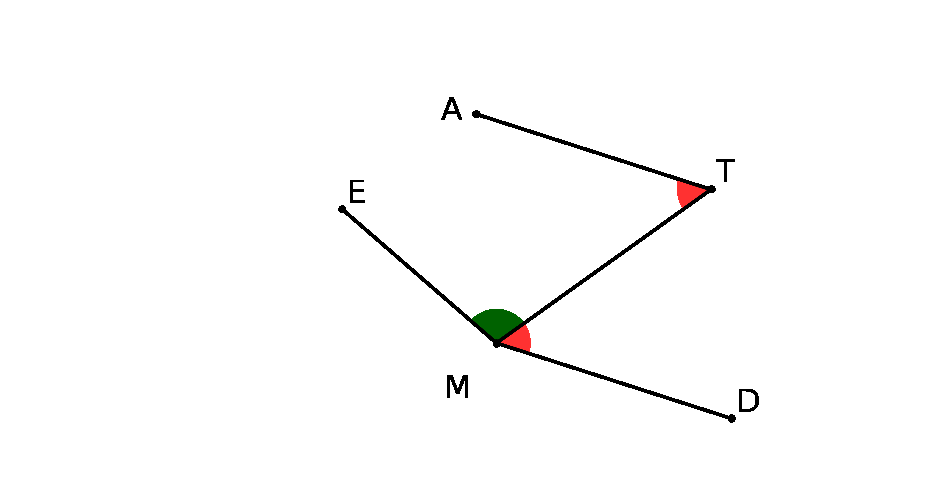
\includegraphics[scale=0.7]{figures/ALJAHW5.eps} \\



 Le th23.1 nous permet de construire, à partir de la droite MT et du point M, le point D tel que A et D sont de part et d'autre de TM et tels que les angles  ATM et TMD sont égaux.\\

 Les angles  ATM et TMD étant égaux le th27.1 implique que les droites DM et AT sont parallèles.\\

La somme des angles EMT et TMD étant inférieure à deux droits, EM et DM forment un angle et T est à l'intérieur de cet angle.\\

PJ implique qu'il existe une droite passant par T et coupant MD et ME respectivement en K et L.\\

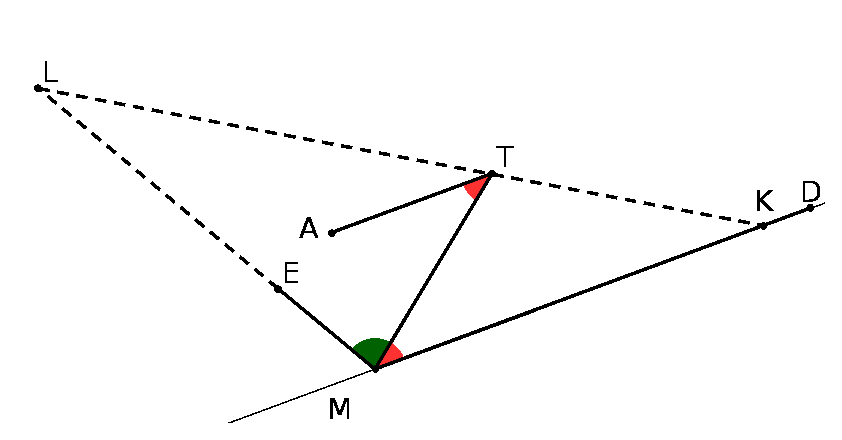
\includegraphics[scale=0.7]{figures/ALJAHW6.eps} \\



L et E sont du même côté de MT. Sinon, L serait sur KT, donc, d'après P8, ME couperait MT, en un autre point que M, donc MT serait distincte de MT avec deux points commun: impossible d'après P6.\ 

MD étant parallèle à AT, M et D étant du même côté de AT,  K l'est aussi.\

Donc KT coupe AT et K et L sont de part et d'autre de AT. Il en est donc de même de E et L, donc EL coupe AT, donc ME et AT se coupent.\


  
  \newpage \section{PJ est-il indépendant de P5?}\
  
  \textbf{Tout d'abord P5 implique PJ}. En effet soit un angle BOC et un point A à l'intérieur de cet angle.\
  
  On prend deux points D et E, D sur OB et E sur OC. On trace DE puis la parallèle (d) à DE passant par A.\
  
  Si (d) est parallèle à OB alors il existerait deux parallèle à (d) passant par D: la droite DE et la droite OB. Or d'après P5 il n'existe qu'une seule parallèle à une droite donnée. Donc (d) coupe OB. De même (d) coupe OC. Ainsi PJ est démontrée.
  

  
  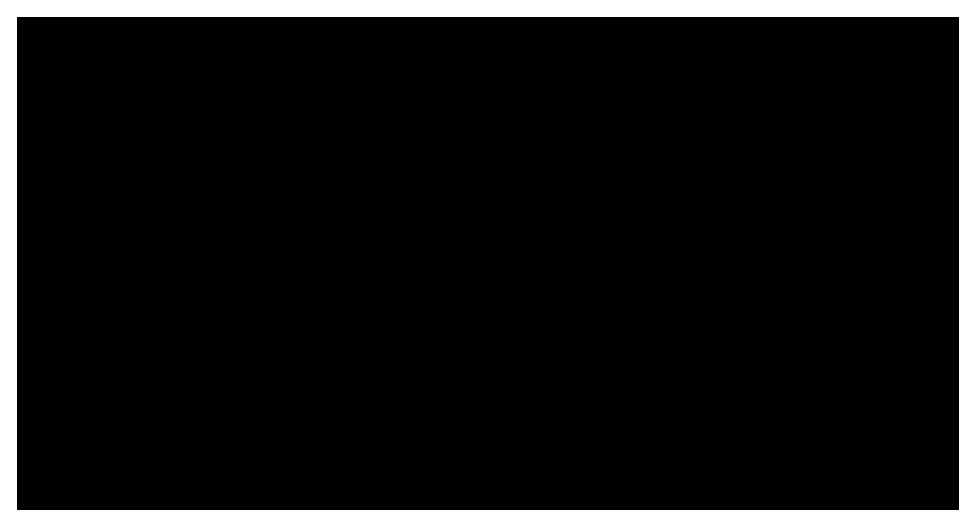
\includegraphics[scale=0.8]{figures/JAHWA3.eps} \
 
 
  \textbf{ Mais pourrait-on démontrer PJ sans P5?}\
   
   On prend, comme précédemment, un angle BOC et un point A à l'intérieur de cet angle.\
   
   Dire qu'il existe une droite passant par A coupant OB et OC revient à dire qu'il existe un point D de OC tel que la droite DA coupe OB.\
   
    \includegraphics[scale=0.7]{figures/JAHWA4.eps} \
    
    On trace l'angle EDC égal à l'angle BOD (the 23.1). Donc DE et OB sont parallèles (the 28.1). Pour être sûr que AD coupe OB il faut pouvoir affirmer que par D il n'existe pas deux parallèles à OB. Ceci est une conséquence de P5. On ne peut pas s'en passer! \\
    
    Ainsi PJ, n'étant qu'une conséquence de P5, n'est pas une piste intéressante.\\
    
    Comment se fait-il que Al Jawhari n'ait pas vu sa faute alors que par ailleurs c'était un grand savant? Sans doute ne pouvait-on pas penser, à cette époque, qu'il était possible de concevoir deux droites sécantes parallèles à une même droite.  
   

\chapter{Al Khayyam:}\

    
 Al Khayyam remplace P5 par l'énoncé suivant (1), qu'on appellera PK:\
 
 \textbf{deux droites concourantes se coupent et il est impossible qu'elles s'écartent l'une de l'autre dans la direction où elles concourent. }\
 
 Cet énoncé ne dit pas autre  chose que P5! et naturellement Al Khayyam en déduit que \textbf{deux droites perpendiculaires sont équidistantes.} \
 
 Cependant sa démarche est intéressante parce qu'il va démontrer P5 par l'absurde et poser des hypothèses qui serviront pour créer des géométries non euclidiennes.
 
 \section{le quadrilatère de Al Khayyam:}\
 
 
  Rappelons que le théorème 4.1 nous permet d'affirmer que deux triangles, ayant un angle égal entourés par deux côtés égaux, sont égaux.\
  
  Rappelons aussi que les th.10.1 et 11.1 nous permettent de tracer des perpendiculaires et que le th13.1 nous permet d'affirmer qu'une droite coupant une autre fait soit deux angles droits, soit deux angles, qui réunis, font deux droits.\\
  
  
 
 \includegraphics[scale=0.6]{figures/KHAYYAM.eps}\
 
 \footnote{ce principe est celui énoncé par Aristote dans un traité dont parle Al Khayyam mais qui ne nous est pas parvenu }  
 
 
  Il construit la droite AB puis il mène les perpendiculaires BD et AC, (th11.1), telles que BD=AC.\\
  
  
 \includegraphics[scale=0.6]{figures/KHAYYAM.eps}\\
 
 Pour nous il est évident que ce quadrilatère est un rectangle. Cependant cette "évidence" est une conséquence de P5, dans les éléments d'Euclide. Donc Al Khayam ne l'admet pas.\\
 
 
 
  
  Il commence par démontrer que les angles BDC et ACD sont égaux.\
 

 
 Voici une démonstration possible:\ 
 
 1. On a $BD=AC$, $BA=AB$, D\^{B}A=C\^{A}B donc (th4.1)  $AD=CB$.\
 
 2. On démontre de même que  les triangles DAC et CDB sont égaux donc leurs angles sont égaux deux à deux (th4.1).\
 
 3. On en déduit que les angles BDC et ACD sont égaux.\\
 
 
 Puis Al Khayyam élève la perpendiculaire à AB en son milieu E (th 10.1 et th 11.1) et il démontre que EG est perpendiculaire à CD et que G est le milieu de CD.\\
 
  \includegraphics[scale=0.7]{figures/KHAYYAM1.eps} \\
  
 
 Voici une démonstration possible:\\

  
 
 1. On démontre que les triangles BGE et AGE sont égaux (th 4.1).\
 En effet: $EG=EG$,$EB=EA$ et $GEB=GEA=1$ droit. Donc BG=AG.\
 
 
 2. Puis que les triangles BDG et CGA sont égaux.\ 
 
 En effet: $BG=GA$, $BDG=ACG$ et $DBG=CAG$ puisque \
 
 $DBG=DBE-GBE=GEA-GAE=CAG$. Donc (th26.1: deux angles et un côté égaux) les triangles sont égaux. Donc DG=GC. Donc G est le milieu de CD. 
 
 3. On en déduit donc que les angles DGE et CGE sont égaux . Donc (th13.1) GE est perpendiculaire à CD.\\
 
 Puis Al Khayyam prolonge EG jusqu'au point K tel que EG=GK. \
 
 Puis il trace la perpendiculaire à EK qui coupe les droites BD et AC quand on les prolonge. Il obtient cette figure. \
 
 \textit{Pour tout un chacun il est évident que la perpendiculaire à EK coupe BD et AC mais, sans P5, rien dans Euclide ne permet de l'affirmer. On pourrait dire que selon PK, les droites se rapprochant elles se coupent...}.\\
 
 
 
  \includegraphics[scale=0.7]{figures/KHAYYAM3.eps}\\
  
  Puis Al Khayyam fait les trois hypothèses suivantes:\
  
  1. H1: les angles C et D sont aigus.\
  
  2. H2: les angles C et D sont obtus.\
  
  3. H3: les angles C et D sont droits.\\
  
  Puis il plie la figure suivant CD, ce qui revient à faire une symétrie orthogonale (mais la notion de transformation n'existe pas encore). On ne détaillera pas mais on peut justifier la figure obtenue par pliage à l'aide d'Euclide sans P5. 
  
  
  Sous H1 on obtient la figure suivante: naturellement elle est déformée!\\
  
  
  
   \includegraphics[scale=0.7]{figures/KHAYYAM2.eps}\\
   
   
   Par pliage F devient S et A devient N. Et naturellement FH=SN. Donc  les perpendiculaires à AB, BD et AC s'écarteraient ce qui contredit le fait que deux perpendiculaires sont équidistantes, conséquence de PK. Donc H1 est impossible.\\
   
   Sous H2 on obtiendrait que les perpendiculaires se rapprocheraient, ce qui est aussi impossible.\\
   
   Sous H3 on n'obtient pas de contradiction.\\
   
   
  Maintenant, une fois démontré cela il est facile de démontrer P5.\\
  
  La démarche de Al Khayyam sera reprise par Saccheri Sept siècles plus tard et il démontrera les premiers résultats de GNE sans le savoir!
   
 
\newpage
 \chapter{Wallis:}
 
 Wallis remplace P5 par l'énoncé suivant qu'on appellera PW:\\
 
 \textbf{ Quel que soit le triangle et quelle que soit la droite il est possible de construire sur la droite un triangle semblable au triangle donné.}\\
 
 Cet énoncé ne fait que généraliser le postulat 3 d'Euclide qui demande de pouvoir tracer un cercle quel que soit le rayon, ce qui signifie que l'on peut tracer des cercles semblables.\
 \section{PW est-il vraiment indépendant de P5?}
 
  
 Wallis pensait évident que son énoncé était indépendant de P5 et que l'on pouvait le rajouter à la géométrie neutre sans avoir à démontrer quelque chose.\
 
 Or PW est un cas particulier du théorème 18 du livre VI d'Euclide. La démonstration de ce théorème utilise le fait que la somme des angles dans un triangle est égale à deux droits  et... PW est une conséquence de P5 et il ne peut pas en être autrement. En effet:\\
 
  soit un triangle ABC et une droite DE. Construisons un triangle semblable à ABC, de base DE. \
  
  Deux méthodes: soit on travaille sur les angles, soit on introduit  les côtés proportionnels.\
  
 \subsection{ D'abord par les angles:}
  
  
\includegraphics[scale=0.7]{figures/WALLIS1.eps} \\

On sait construire les angles D et E égaux respectivement à CAB et CBA (th23.1). On sait (th 17.1) que CAB et CBA sont plus petits que deux droits et les droites se coupent si on admet P5. Donc, par les angles on utilise P5.\\

\subsection{Essayons par la proportionnalité.}
 

 Soient de nouveau un triangle ABC et une droite DE et essayons de construire un triangle semblable à ABC sans P5.\

On construit l'angle D égal à CAB (th 23.1) puis on trace  DF=AC et DG=AB (Th2.1). On obtient le triangle DFG égal à ABC (Th4.1).\\


 \includegraphics[scale=0.7]{figures/WALLIS2.eps} \\
 
 
 
 
  Puis on trace GF et "une" parallèle à FG passant par E, EH, (on ne peut pas dire "la" parce que l'unicité de la parallèle se déduit de P5. Voir la démonstration dans celle du théorème 30 (début du chapitre) . Il faut démontrer ensuite que EH coupe proportionnellement DF et DG. Malheureusement pour Wallis il s'agit de th 2.6 dont la démonstration utilise plusieurs théorèmes conséquences de P5!\\
  
  
  
  Donc admettre PW sans chercher le lien qu'il pourrait avoir avec P5 est étonnant!  D'autant plus que Wallis devait connaitre parfaitement les Eléments d'Euclide. Mais rappelons encore que nous sommes dans le siècle de Descartes et Newton et que, contrairement aux grecs on ne se pose pas le problème du fondement des mathématiques. PW semble tellement évident que l'on ne peut que l'admettre.\\
 
 Voyons maintenant comment on peut démontrer P5 à partir de PW.
 
 \section{PW implique P5:}
 
 
\subsection{Somme des angles dans un triangle:}\
 
 \paragraph{Triangle rectangle:}\
 
 
 Soit un triangle MNP rectangle en P et soit une droite AB. On trace (PW) le triangle ABC semblable à MNP rectangle en A, de dimension double. Puis on trace le triangle BC'B' égal au triangle MPN. Puis on trace la perpendiculaire B'H à AC.\\
 
  
 \includegraphics[scale=0.5]{figures/WALLIS3.eps} \\
 
 Cette construction s'est faite en utilisant uniquement PW et les théorèmes ne nécessitant pas P5.\
 
 1. Les triangles BB'C' et B'HC sont égaux: (th 26.1) ils ont en effet deux angles égaux et un côté égal.($C=B'$, $H=C'$ et $B'C=BB'$).\
 
 2. Donc $HB'=AC'=BC'$, $CH=AH=B'C'$.\
  
  
  3. Donc les triangles B'HC' et HAC' ayant trois côtés égaux sont égaux (th8.1) et donc $HB'C'=HAC'=$1 droit.\\
 
  \includegraphics[scale=0.4]{figures/WALLIS4.eps} \\
  
 
  
  4. Comme $CB'H+HB'C'+C'B'B$=2 droits\
  
  d'où $CB'H+C'B'B$=1 droit. 
  
  5. Donc la somme du triangle MNP est égale à 2 droits.
  
 \paragraph{Triangle quelconque:}\
 
   Pour un triangle quelconque on se ramène à deux triangles rectangles, donc la somme de ses angles est aussi égale à deux droits.\
   
  \newpage  \subsection{Démonstration de P5:}
    
    \textbf{Théorème 6.1:} Si deux droites sont parallèles toute droite qui coupe l'une coupe l'autre.\\

    
      
  
 \textit{Démonstration:} Soient AB et CD deux droites parallèles, E un point de CD et EF1 une droite coupant CD.\
 
 Soient EG la perpendiculaire à AB et F1H1 la perpendiculaire à EG (th 12.1).\
 
 On prolonge EF1 en EF2 tel que $EF1=F1F2$ et on trace la perpendiculaire F2H2. \
 
 La somme des angles étant égale à 2 droits les triangles EF1H1 et EF2H2 ont leurs angles égaux donc sont semblables et donc leurs côtés sont proportionnels. Ainsi $EH1=H1H2$.\\

 
 
 \includegraphics[scale=0.6]{figures/WALLIS5.eps} \\
 
 
  En itérant cette construction on obtient une suite de points Hi tels que, pour tout $n$ :$HnHn+1=EH1$.\
 
 Il existe $n$ tel que $EHn>EG$. EHn coupant AB et FnHn perpendiculairement, les droites AB et HnFN sont parallèles (th28.1). Donc les points E et Fn sont de part et d'autre de AB donc EFn coupe AN. D'où le résultat.\\
 
  \includegraphics[scale=0.5]{figures/WALLIS6.eps}\\
  
  
  \newpage \paragraph{Démontrons P5:}\
  
  Soient deux droites AC et BD coupant la droite AB telles que les angles CAB et DBA sont ensemble plus petits que deux droits. \\
 
  
  \includegraphics[scale=0.7]{figures/WALLIS7.eps}\\
  
   
  On prolonge AB en BF et on construit l'angle EBF égal à CAB. \
  
  D'après le th 28.1, EB et CA sont parallèles et les droites BD et BE ne sont pas confondues: en effet, si cela était le cas les angles CAB et DBA, ensemble, seraient égaux à deux droits.\
  
  Donc BD coupe BE et donc coupe aussi AC. Ce qu'il fallait démontrer.
  
 
\chapter{SACCHERI:(1)}\
 
 Saccheri prend donc un quadrilatère ABDC, celui de Al Khayam, dans lequel les angles A et B sont droits et les côtés AC et BD sont égaux. Ce quadrilatère est appelé quadrilatère de Saccheri. On le notera \textbf{S-q}\
 
 Naturellement, pour nous, il est évident que les angles C et D sont droits. Mais pour affirmer cela il faut utiliser le fait que deux droites parallèles sont équidistantes. Or ce résultat découle de P5 et c'est justement P5 que Saccheri veut démontrer! Ainsi , si l'on sait que les droites AC et BD sont parallèles (th27) on ne sait rien de plus.\
 
 Dans ce chapitre on garde, du livre 1, toutes les définitions, les postulats, excepté P5, et tous les axiomes, et enfin les vingt huit premiers théorèmes, ceux qui ne dépendent pas de P5.\
 
 Nous allons essayer, à partir de là, de démontrer des résultats de Saccheri.
   
 \footnote{(1) on peut se référer au livre de Barbarin: \textit{La géométrie non euclidienne 1907} ou à  Beltrami qui a découvert et fait connaître les travaux de Saccheri ou encore à Voelke: \textit{Renaissance de la géométrie non euclidienne}  ou encore à tous les articles qui ont été écrits sur le sujet! } 


\newpage \section{Premiers résultats:}\





\textbf{Proposition 7.1: dans un S-q, ABDC, les diagonales sont égales, les angles C et D sont égaux et si on appelle O le point d'interchapter des diagonales, les triangles OCD et OAB sont isocèles}.\\

\includegraphics[scale=0.5]{figures/sacc1.eps}\\

\textit{Remarque: Quel que soit le prolongement de AC ou BD, cette figure existe d'après Th 28.1: deux doites perpendiculaires sont parallèles}

Les triangles CAB et DBA sont égaux (th4.1): \
 
En effet: $AC=BD$, $AB=BA$, $\hat{DBA}=\hat{CAB}$ (th4.1).\ 

Donc, en particulier, $BC=AD$ et les égalités d'angles marqués sur la figure.\\




Puis on démontre l'égalité des triangles DCA et CDB: en effet: \

$CA=DB$, $AD=BC$, $DC=CD$. D'où, en particulier: $\hat{DCA}=\hat{CDB}$ et les autres angles marqués sur la figure qui suit.\

En conclusion : on sait que les angles C et D du quadrilatère sont égaux mais on ne connaît pas leur valeur. 

\includegraphics[scale=0.5]{figures/sacc3.eps}\


\textbf{Proposition 7.2: soit un S-q, ABDC, et soient deux points E et F respectivement sur AC et BD, prolongées ou non, tels que AE=BF. Alors les diagonales de CEFD sont égales, et si on appelle O le point d'interchapter des diagonales, les triangles OEF et OCD sont isocèles.  }\\

La démonstration est la même que pour la proposition 1.\\

Le quadrilatère ABFE est un S-q donc les angles E et F sont égaux.\\

\includegraphics[scale=0.5]{figures/sacc6.eps}\

En effet les triangles CEF et DFE sont égaux puisque:\

1. $C\hat{E}F=D\hat{F}E$.\

2. $CE=DF$ et $EF=FE$.\

les triangles CED et CDF sont égaux puisque:\

1. $E\hat{C}D=C\hat{D}F$.\

2. $CE=DF$ et $CD=DC$.\

Donc, en particulier les diagonales CF et ED sont égales et les triangles OCD et OEF sont isocèles.\\





 \textbf{Proposition 7.3: soit S-q, ABDC, et soient I et J les milieux respectifs de AB et CD . Alors IJ est perpendiculaire à AB et CD et passe par le point d'interchapter des diagonales. En particulier AB et CD sont parallèles. }\\

\textbf{De plus si E et F sont définis comme dans la proposition 2, IJ passe par le point d'interchapter des diagonales du quadrilatère EFDC. }\\

\includegraphics[scale=0.5]{figures/sacc7.eps} \\


Rapidement:  le triangle OAB est isocèle et donc la droite OI est perpendiculaire à AB (On ne fait qu'appliquer des théorèmes de 1 à 28 du livre 1).\

La droite OI coupe l'angle AOB en deux angles égaux. De même la droite OJ coupe l'angle COB en deux angles égaux.\

 Les angles COA et DOB sont égaux donc les angles COJ et DOJ sont égaux aux angles AOI et BOI. Donc les angles JOC, COA et AOI, pris ensemble, sont égaux aux angles JOD, DOB et BOI, pris ensemble. Donc I, O et J sont alignés.\\
 

IJ, étant la médiatrice des segments AB et CD, O' est sur IJ. \\



IJ étant une perpendiculaire commune à AB et CD, les droites AB et CD sont parallèles (th 27.1).\\

\section{Hypothèses de Saccheri.}






A partir de son quadrilatère Saccheri émet les trois hypothèses suivantes:\

H1: C et D sont droits.\

H2: C et D sont obtus.\

H3: C et D sont aigus.\

Puis il espère, sous H1, démontrer P5 et  arriver, sous les hypothèses H2 ou H3, à une contradiction. Donc, seule la géométrie euclidienne serait valide et P5 serait démontré!\


\section{On se place sous H1:}\


\subsection{On va démontrer que s'il existe un S-q dont les quatre angles sont droits alors tous les S-q sont des rectangles.}
\



\textbf{Lemme 1:} Soit AB une droite et E n'appartenant pas à cette droite. On appelle F le point de AB tel que EF est perpendiculaire à AB. Soit M un point quelconque de FA. Alors l'angle EMA est obtus et l'angle EMB aigu.\\

\textit{Démonstration:} \

\includegraphics[scale=0.7]{figures/saccheri1.eps} \\

Rappelons le th16.1:le côté d'un triangle étant prolongé, l'angle extérieur est plus grand que chacun des angles opposés et intérieurs.\\

EF existe d'après Th12.1 et le résultat est une application de Th.16.1.\\

\textbf{Lemme 2:} si dans un S-q, ABDC, tel que AC=BD, il ya quatre angles droits alors AB=CD.\\

\textit{Démonstration:} D'après P.7.1, les diagonales AD et BC sont égales. Les  triangles ACD et ACB  sont égaux (un angle et deux côtés égaux) donc on en déduit que AB=CD.\\

\textbf{lemme 3:} soit un rectangle ABDC et soit E un point de AC. Soit F le point de BD tel que EF est perpendiculaire à BD. Alors l'angle FEA est droit.\\

 \includegraphics[scale=0.7]{figures/saccheri2.eps} \\

\textit{Démonstration:}\

Supposons l'angle AEF aigu.\
 
 On place sur BA (prolongée ou non) à partir de B le point E' tel que BE'=EF. Alors BFEE' est un quadrilatère de Saccheri. Donc les angles FEE' et BE'E sont égaux. Supposons que E' soit sur AB (n'oublions pas que les droites sont finies).\\
 
  
 \includegraphics[scale=0.8]{figures/saccheri3.eps} \\
 
  On a supposé l'angle FEA aigu donc l'angle FEE' est aigu. Mais d'après le lemme 1 BE'E est obtus. Or ces deux angles sont égaux donc E' n'est pas sur AB donc $EF>AB$.\\
  
  

Raisonnons maintenant sur le quadrilatère EFDC. On place E" sur DC prolongé, à partir de D, tel que DE"=EF. Comme on a supposé l'angle FEA aigu, l'angle FEC est obtus.\\

\includegraphics[scale=0.8]{figures/saccheri2bis.eps}

 Donc, puisque EFDE" est un S-q, les angles FEE" et DE"E sont égaux. Comme l'angle FEE" est plus grand que FEC, il est obtus. D'après le lemme 1, c'est impossible donc E" est sur DC, donc $DE"<DC$ donc  $EF<CD$. \\

Donc $AB<EF<CD$. Donc $AB<CD$. Or ABDC est un rectangle donc AB=CD. Donc l'angle FEA ne peut être aigu. De même il ne peut être obtus. Donc il est droit.\\
 
\textbf{Lemme 4:}  soit un rectangle ABDC et soit E un point sur AC prolongée du côté de C. Soit F le point de BD tel que EF est perpendiculaire à BD. Alors l'angle FEA est droit.\\

\textit{Démonstration:}\\

  \includegraphics[scale=0.7]{figures/saccheri4.eps}\\
  
  On va se ramener au lemme 3.\
  
  D'après P2 on peut prolonger continûment une droite. Donc Prolongeons AC du double ainsi que BD. On obtient la figure suivante:\\
  
   \includegraphics[scale=0.9]{figures/saccheri5.eps}\\
   
   On démontre facilement l'égalité des triangles ABC, ABD, CAD, CBD, CJD, IDC d'où on en déduit l'égalité des angles indiqués sur la figure.\\
   
  
  
   
   L'angle ICD est droit donc ICJ et CID sont égaux donc les triangles ICJ et ICD sont égaux donc les angles IJC et IDC aussi. Comme les angles IDC DIC pris ensemble sont égaux à un droit, l'angle IJD est droit donc AIJ aussi, puisque ABJI est un S-q, donc  ABJI est un rectangle.\\
   
   En recommençant cette opération autant de fois qu'il le faut, on peut supposer que le point E, même s'il est le prolongement de AC, appartient au côté d'un rectangle. Ainsi l'angle FEA est droit.\\
   
 \textbf{Proposition 7.4:} S'il existe un S-q qui est un rectangle tous les S-q le sont aussi.\\

\textit{Démonstration} soit ABDC un rectangle et E'F'T'G' un S-q.\\

 \includegraphics[scale=0.7]{figures/saccheri6.eps}\\

1. ABDC pouvant être agrandi autant de fois qu'on le veut, on peut supposer que    $E^{'}F^{'}<AB$ et $E^{'}G^{'}<AC$. Ainsi construisons le S-q AFHG tel que AF=E'F', AG=E'G'. On obtient la figure suivante:\\

  \includegraphics[scale=0.7]{figures/saccheri6.eps}\\   
   
   Soit H' le point de CD tel que FH' est perpendiculaire à CD. Mais d'après le lemme 3 cela implique que l'angle AFH' est droit donc F, H et H' sont alignés. Donc AFH'C est un rectangle.\\
   
2. Soit G' le point de FH' tel que GG' est perpendiculaire à FH'. Alors, d'après le lemme 3, l'angle AGG' est droit.\

 Si on suppose que l'angle AGH est aigu, alors G' est sur HH' et donc l'angle GHF est obtus: c'est impossible puisque les deux angles AGH et GHF sont égaux. Si on suppose que l'angle AGH est obtus, alors l'angle GHF est aigu: c'est impossible. Donc AFHG est un rectangle. \\

\textit{Remarque: on pourrait se demander si avec la construction ci-dessus les S-q, AFHG et E'F'T'G', sont égaux. Pour s'en persuader il suffit de considérer les égalités des triangles des deux figures. Donc les deux S-q auront les mêmes angles au sommet.}\\

\textbf{Corollaire 7.4:} Si un quadrilatère a trois angles droits le quatrième angle est aussi droit.\\

\textit{Démonstration:}\

\includegraphics[scale=0.5]{figures/saccheri7.eps}\\

Soit D' tel que AD'=BD. Alors ABDD' est un S-q donc l'angle BDD' est droit donc C=D'. D'où le résultat.\\

   
   
   

\newpage  \subsection{Somme des angles d'un triangle:}
 
 
 
\textbf{Proposition 7.5: la somme des angles d'un triangle est égale à deux droits.}\\
 
 
\textbf{1.} Soit ABC un triangle rectangle et A. On trace la perpendiculaire à AB en B, BD,  telle que BD=AC. Donc ABDC est un S-q donc un rectangle dont la somme des angles est égale à 4 droits.\\


  \includegraphics[scale=0.5]{figures/saccheri1bis.eps}\\
  
 Les triangles ABC et BCD sont égaux donc la somme des angles de ABC est égale à deux droits.\\ 


 \textbf{2.} Prenons d'abord un triangle ABC de hauteur CE, E étant sur AB ou sur son prolongement. \
 
 \textbf{a.} Si E est sur AB:\\
 
 
  \includegraphics[scale=0.5]{figures/saccheri1ter.eps}\\
 
 La somme, S, des angles de ABC est:\
 
  S=1+2+3+4=(1+4+1droit)+(2+3+1droit)-2droits= 2 droits si on applique \textbf{1.}\\
  
 \textbf{b.}  Si E est sur le prolongement de AB:\\
 
 \includegraphics[scale=0.5]{figures/saccheri1quater.eps}\\ 
 
 les triangles ACE et BCE sont rectangles donc on a:\
 
 1+2+4=2+5 donc 1+3+4+2=2+3+5 donc 1+3+4= 2 droits d'où le résultat.\\
 
 
 

 
 \subsection{Démonstration de P5:}
 
 
  
  \textbf{Proposition 7.6: P5 est vrai.}\\
  
  Saccheri montre d'abord le résultat suivant.\\

  
 \textbf{lemme: soient trois droites AC, AB, BD telles que BD est perpendiculaire et l'angle CAB est aigu. Alors AC et BD se coupent.} \\
 
 
\includegraphics[scale=0.7]{figures/sccH1a.eps} \\
 
 

 

 
Soient $M_{1}$,$M_{2}$,$M_{3}$ trois points de AC tels que $AM_{1}=M_{1}M_{2}=M_{2}M_{3}$. Et on trace les perpendiculaires $M_{1}N_{1}$, $M_{2}N_{2}$, $M_{3}N_{3}$.\

On trace la perpendiculaire $M_{1}E$ à $M_{2}N_{2}$.\


 

 
 Le quadrilatère M1N1N2E a trois angles droits donc (Corollaire 7.4) l'angle $N_{1}M_{1}E$ est droit. Donc la somme des angles $AM_{1}N_{1}$ et $M_{2}N_{1}E$ est égale à un droit.\
 
 La somme des angles d'un triangle étant égale à deux droits, les angles $M_{2}M_{1}E$ et $AM_{1}N_{1}$ sont égaux.\
 
  Les triangles rectangles $AM_{1}N_{1}$ et $M_{1}M_{2}E$, ayant un côté et un angle égal, sont égaux. Donc  $M_{1}E=N_{1}A$.  On en déduit que $M_{1}E=N_{1}N_{2}=M_{1}E$. Donc  $N_{1}N_{2}=N_{1}A$.\
  
 On démontrerait de même que $N_{1}N_{2}=N_{2}N_{3}$.\\
 
 
 En construisant la suite de points $M_{n}$ tels que $M_{n}M_{n+1}=M_{n+1}M_{n+2}$ on définit ainsi une suite de segments égaux $N_{n}N_{n+1}$. Il existe alors une valeur de $n$ telle que $AN_{n}\leq AB$ et$AN_{n+1}> AB$ ( la géométrie euclidienne est archimédienne). $M_{n+1}N_{n+1}$ étant parallèle à BD $M_{n+1}$ et $M_{n}$ sont de part et d'autre de BD donc AC coupe BD.\\
 
\textbf{Démontrons maintenant P5.}\\

 
 Soient une droite AB tombant sur les droites AC et BD en faisant des angles plus petits que deux droits. L'un des deux angles est aigu. Supposons que c'est l'angle DBA. Alors la perpendiculaire AE à BD a son pied E entre B et D (Quitte à prolonger BD).\
 
 a. Si $\hat{CAB}<\hat{EAB}$ alors AC coupe l'angle $\hat{EAB}$ donc AC coupe BE donc BD. (C'est une affirmation non démontrée qu'il faudrait rajoutée sous la forme d'un postulat dans les Eléments d'Euclide, manque déjà indiqué à l'occasion de l'énoncé du th 21.1)\\
 
 b. Si $\hat{CAB}=\hat{EAB}$ alors AC coupe BD en E.\\
 
 c. Supposons $\hat{CAB}>\hat{EAB}$.\\
 
 
 \includegraphics[scale=0.6]{figures/saccH1b.eps} \
 

 
 La somme des angles est égale à deux droits donc $\hat{DBA}=$1droit$-\hat{BAE}$ et les deux angles sont aigus.\ Or:\
 
 $\hat{DBA}+\hat{CAB}< 2 $droits. Donc\
 
 1 droit-$\hat{BAE}+\hat{CAB}<$ 2 droits. Donc\
 
 $0<-\hat{BAE}+\hat{CAB}< $1 droit. Donc\
 
 $\hat{CAE}< 1 $ droit. Et d'après le résultat préliminaire, DE coupe AC donc BD et AC se coupent. \\
 
 
 
 \newpage  \section{On se place sous H2:}\
 
 Si ABDC est un S-q dans lequel les angles A et B sont droits, on suppose que C et D sont obtus.
  
\subsection{Résultats préléminaires:}

\textbf{ Proposition 7.7: sous H2, dans un S-q ABDC tel que AC=BD, on a:  $CD<AB$ et si on appelle E le point d'interchapter des diagonales on a $EC<EB$. }\\

\textit{Démonstration:}
 
 1. Soient I et J les milieux respectifs de AB et CD. Alors IJ est perpendiculaire à CD (P.7.3).\\
 
   \includegraphics[scale=0.7]{figures/sacc132.eps}\\
   
 Supposons $AI<CJ$. Soit G tel que GJ=AI et G sur CJ. Alors IJAG est un S-q donc les angles $\hat{JGA}$ et $\hat{IAG}$ sont égaux (P.7.1). Or  
   $\hat{IAG}$ est aigu puisque $\hat{IAC}$ est droit et $\hat{JGA}$ est obtus puisque $\hat{JCA}$ est obtus. C'est impossible puisque   $\hat{IAG}=\hat{JGA}$. Donc contradiction et on n'a pas $AI<CJ$.\\
   
   On ne peut pas avoir non plus AI=CJ: en effet IJCA serait un S-q et donc l'angle A serait égal à l'angle C d'après P.7.1. L'angle A étant droit, l'angle C le serait aussi: impossible.\\
   
   On a donc $CJ<AI$ donc $CD<AB$.\\
   
   Traçons les diagonales BD et AC qui se coupent suivant un point E qui est sur IJ (P.7.3).\\
   
    \includegraphics[scale=0.7]{figures/sacc133.eps}\\
    
    Supposons $ED>EA$.\
    
    Soit F, le point de EA prolongée en A, tel que EF=ED et soit FG la perpendiculaire à IJ. Alors les triangles EFG et JED sont égaux (Th 26.1: deux angles et un côté égal). Donc JD=FG.\
    
    Dans le triangle JDE l'angle J est droit donc (Th17.1: la somme de deux angles dans un triangle est inférieure à deux droits) l'angle $\hat{JDE}$ est aigu, donc $\hat{EFG}$ aussi.\
    
    Soit H tel que AI=GH. Alors IGHA est un S-q et donc $\hat{IAH}=\hat{GHA}$. H est sur FG et distinct de F, sinon $\hat{IAH}$ serait obtus: en effet $\hat{IAC}$ est droit donc $\hat{IAD}$ est aigu donc $\hat{IAF}$ est obtus donc $\hat{IAH}$ et $\hat{GHA}$ le seraient aussi. Mais $\hat{GHA}$ serait aigu puisque $\hat{GFA}$ est aigu. Donc, impossible.\
    
    Donc $AI<FG$ puisque GH=AI. Donc $JD>AI$: impossible, puisque $CD<AB$. Donc $ED<EA$.\\
    
   

\newpage \textbf{Théorème:} si un S-q vérifie H2 il en est de même  de tous les S-q.\\

\textit{Démonstration:}\\

Commençons par les lemmes suivants:\\

\textbf{Lemme 1:} soit ABDC un S-q vérifiant H2 et tel que AC=BD. On appelle I et J les milieux respectifs de AB et CD.\

1. Alors $IJ>BD$.\

2. Soit E un point de CD et soit EF la perpendiculaire à AB. Alors $EF>BD$.\\

\textit{Démonstration:}\

 \includegraphics[scale=0.7]{figures/sacc134.eps}\\ 
 
 1. Supposons $IJ\leq BD$. Alors il existe un point H de BD tel que IJ=BH. IBHJ est un S-q et on a $\hat{IJH}=\hat{BHI}$. Comme $\hat{IJH}$ est aigu ou droit, $\hat{BHI}$ l'est aussi. Or $\hat{BDJ}$ est obtus donc $\hat{BHI}$ aussi: contradiction. Donc $IJ>BD$.\\
 
 2. Supposons $EF<BD$. Soit G le point de FE prolongée tel que FG=BD. les quadrilatères AFGC et FBDG sont des S-q donc $\hat{FGD}=\hat{BDG}$ et $\hat{ACG}=\hat{FGC}$. Or F et G sont de part et d'autre de CD, donc  $\hat{ACG}>\hat{ACD}$ et $\hat{BDG}>\hat{BDC}$. Comme les angles $\hat{ACD}$ et $\hat{BDC}$ sont obtus il en est de même de $\hat{ACG}$ et $\hat{BDG}$. Donc $\hat{CGD}$ serait plus grand que deux droits:  impossible.\
 
 Si EF=BD alors EF=AC. Donc les quadrilatères AFEC et FBDE sont des S-q donc $\hat{FED}=\hat{BDE}$ et $\hat{ACE}=\hat{FEC}$. Comme les angles $\hat{ACD}$ et $\hat{BDC}$ sont obtus il en est de même de $\hat{ACE}$ et $\hat{BDE}$: impossible.\
 
 Donc $EF>BD$.\\
 
 
 \textbf{Lemme 2:} soit ABDC un S-q vérifiant H2 et tel que AC=BD. On appelle I et J  les milieux respectifs de AB et CD. \
 
 1. Soit G le point de IJ tel que IG=AC. Alors AIGC et IBDG sont des S-q vérifiant H2.\
 
 2. Soit F un point de AB, distinct de B, et soit le point E tel que EF=AC, EF perpendiculaire à AB et C et E du même côté de AB. Alors AFEC et FBDE sont des S-q vérifiant H2.\\
 
   \textit{Démonstration:}\\
   
 1. Soit la figure suivante:\\
 
  \includegraphics[scale=0.7]{figures/sacc137bis.eps}\\
 
 a. D'après le lemme 1, IJ$>$AC donc G$\in$IJ. \
 
 b. Les quadrilatères AIGC et IBDG sont égaux.\
 
 c. L'angle $\hat{CGD}$ est plus petit que deux droits. Donc le double de l'angle $\hat{CGI}$ est plus grand que deux droits donc $\hat{CGI}$ est obtus. ainsi AIGC et IBDG sont des S-q vérifiant H2.\\
 
 2. Supposons que F$\in$IB.\\
 
 
  \includegraphics[scale=0.7]{figures/sacc137.eps}\\

  a. Si E et F sont de part et d'autre de CD alors EF couperait CD en un point H et, d'après le lemme 1, FH serait plus grand que BD, donc aussi EF: contradiction. Donc E et F du même côté de CD.\

EF, IJ et BD sont parallèles (Th28.1) donc E est à l'intérieur de IBDJ.\

E et C sont de part et d'autre de IJ. Donc EC coupe IJ en un point G.\\



En utilisant l'égalité des triangles AIG et BIG, puis celle des triangles ACG et BDG, on démontre que $\hat{ACG}=\hat{BDG}$.\

Supposons $\hat{ACE}$ aigu. Alors $\hat{BDG}$ l'est aussi. $\hat{BDE}<\hat{BDG}$ donc $\hat{BDE}$ est aigu. Donc les angles $\hat{CEF}$ et $\hat{DEF}$ le sont aussi: impossible, sinon $\hat{CED}$ serait plus grand que deux droits. Donc $\hat{ACE}$ est obtus. Donc AFEC est un S-q vérifiant H2.\\

b. Montrons que IBDG est aussi un S-q vérifiant H2.\

Soient les suites de points I$_{n}$, G$_{n}$, J$_{n}$ telles que:\

(i) I$_{0}$=I, J$_{0}$=G$_{n}$=J.\

(ii) pour tout $n>$0, I$_{n}$ est le milieu de I$_{n-1}$B, G$_{n}$ est le point de I$_{n-1}$J$_{n-1}$ tel que I$_{n-1}$G$_{n}$=AC et J$_{n}$ est le milieu de G$_{n}$D.\\


  \includegraphics[scale=0.7]{figures/sacc137ter.eps}\\
 
 
 D'après le 1. du lemme, I$_{n}$BDG$_{n+1}$ et I$_{n-1}$I$_{n}$G$_{n+1}$G$_{n}$ sont des S-q vérifiant H2.\
 
 Il existe $n$ tel que F$\in$I$_{n-1}$I$_{n}$. Alors, comme dans le a. on démontre que FBDE est un S-q vérifiant H2.\\ 
 
 
\newpage \textbf{Lemme 3:} soient ABDC et BFED des S-q  tels que AC=BD=EF et tels que A, B et F sont alignés. Si ABDC vérifie H2 alors BFED et AFEC le sont aussi.\\

\textit{Démonstration:}\

1. Si F est sur AB:\\

 \includegraphics[scale=0.7]{figures/sacc170.eps}\\
 
 Alors d'après le lemme 1, E est à l'intérieur de ABDC et, d'après le lemme 2 BFED et AFEC sont des S-q vérifiant H2.\\
 
 2. Si F est sur le prolongement de AB prolongée en B:\

a. Si AB=BF:\\

\includegraphics[scale=0.5]{figures/sacc170bis.eps}\\

ABDC et BFED sont égaux donc BFED vérifie H2. Donc les angles $\hat{FED}$ et $\hat{BDE}$ sont obtus. Donc l'angle $\hat{CDE}$ est plus petit que deux droits. Donc la droite CD coupe l'angle$\hat{ACE}$. \

L'angle $\hat{ACD}$ est obtus donc $\hat{ACE}$ aussi, donc AFEC est un S-q vérifiant H2.\\

b. Si AB$\neq$BF:\

On double AB autant de fois pour obtenir un S-q, AHLC, vérifiant H2 et tel que F soit sur AH.\\

\includegraphics[scale=0.5]{figures/sacc170ter.eps}\\

Alors d'après le 1. on a le résultat souhaité.\\
 
 


 
 
 

\textbf{Lemme 4:} soit ABDC un S-q vérifiant H2 et tel que AC=BD. Soient E et F les points de AC et BD (éventuellement prolongées) tels que AE=BF.  Alors le quadrilatère ABFE est un S-q vérifiant H2.\\

\textit{Démonstration:}\

On appelle I, J et K les milieux respectifs de AB, EF et CD.\

1. Supposons que E soit sur AC.\\

 \includegraphics[scale=0.7]{figures/sacc231.eps}\\

 
 Soit L le point de CK (éventuellement prolongée en C) tel que KL=AI. Alors AIKL est un S-q. Si L est sur CK alors $\hat{LAI}$ est inférieur à un droit et $\hat{KLA}$ est supérieur à un droit. C'est impossible puisque ces deux angles sont égaux. Donc C est sur LK et $\hat{LAI}$ est obtus, donc AIKL est un S-q vérifiant H2.\
 
  Soit G le point de EJ (éventuellement prolongée en E) tel que GJ=AI. D'après le lemme 2 G est à l'intérieur de AIKL et AGJI est un S-q vérifiant H2. Donc $\hat{IAG}$ et $\hat{AGJ}$ sont obtus. Comme $\hat{IAE}$ est droit, E est sur GJ. \
  
  E est sur GJ et $\hat{AGJ}$ est obtus donc $\hat{AEJ}$ aussi. Donc ABFE est un S-q vérifiant H2.\\
  
2. Supposons que E soit sur AC prolongée.\\  
 
 
 a. Soit L un point de CK, prolongée en C, tel que AI=LJ. On a $CK<AI$ (P.7.7) et $\hat{IAC}$ droit, donc $\hat{IAL}$ est obtus et IKLA est un S-q vérifiant H2.\\
 
  \includegraphics[scale=0.7]{figures/sacc240.eps}\\
 
 Il existe un entier $n$ et un point I' tels que II'=$n$IK et II'$>$IJ. Soit A' tel que AI=A'I' et A'I' perpendiculaire à II'. D'après le lemme 3, II'A'A est un S-q vérifiant H2.\  
 
 L'angle $\hat{IAA'}$ est obtus et $\hat{IAE}$ est droit donc II'A'A contient AC. II' contient J donc II'A'A contient E.\
   
 
  
 
 Soit M, comme indiqué sur la figure, tel que MJ=AI. Alors, d'après le lemme 3, IJMA est un S-q vérifiant H2, donc IAM est obtus donc plus grand que IAE. Donc E est sur JM, donc AEJ est un angle obtus. Donc ABFE est un S-q vérifiant H2. \\
 
 
 \textit{Démonstration du théorème:}\
 
 Soit ABDC un S-q vérifiant H2 tel que AC=BD et soit A'B'D'C' un S-q tel que A'C'=B'D'. Soient G, F et H  tels que\\
 
   \includegraphics[scale=0.6]{figures/sacc233BIS.eps}\\
 
  BG=A'B', et A,B et G alignés dans cet ordre. \
  
  GF=B'D', GF perpendiculaire à AB,  F et C du même côté de AG,\
  
  HG=B'D', H sur BD ou son prolongement.\\
  
 
 \includegraphics[scale=0.6]{figures/sacc233BIS.eps}\\
 
 \textbf{1.} Les quadrilatères BGFH et AGFE sont égaux.\
 
 
 
 \textbf{2.} Soit I le point de GF tel que IG=BD. Alors, d'après le lemme 3, BGID est un S-q vérifiant H2 et donc, d'après le lemme 4, BGFH aussi. Donc A'B'C'D' est un S-q vérifiant H2. \\
 
 
  
 
\newpage \textbf{Proposition 7.8:} Soit ABDC un S-q vérifiant H2 tel que AC=BD. Soit E et F deux points respectivement de AC et BD tels que AE=BF. Alors:\

1. Les diagonales de EFDC se coupent en un point appartenant à IJ, la médiatrice commune de AB et CD.\

2. $CD<EF$ et $OD<OE$\\

\textit{Démonstration:}\


 \includegraphics[scale=0.3]{figures/sacc150.eps}\\

1. a été démontré en P.7.3.\\

2. $\hat{FEC}$ étant aigu (lemme 4), on démontre, comme pour P.7.7, que $ED<EA$.\\
 
 

 
 
    
    
    
  \subsection{Somme des angles dans un triangle:}
      
 
   
  \textbf{ Proposition 7.9: la somme des angles dans un triangle est supérieure à deux droits.} \\
  
   \textit{Démonstration:}\
    
  1.  On prend un triangle ABC rectangle en A. Puis on trace une perpendicu -laire  BD égale à AC.\\
    
           \includegraphics[scale=0.7]{figures/saccH2c.eps}\\
     
      On pose :$\hat{CAB}=d$ et $\hat{BDC}=P$.\
      
    On appelle S la somme des angles de ABC. On a:\
  
   
     $S+\hat{CBD}+\hat{BCD}+P=2d+2P$.\
       
 
    
    Donc\
     
     $S=2d+P-(\hat{CBD}+\hat{BCD})$. Dans le triangle BED, $DE<EB$ donc (Th19.1):\
     
    $\hat{CBD}<\hat{ADB}$ donc $\hat{CBD}<\hat{BCA}$ et on a:  $\hat{BCD}+\hat{BCA}=P$ donc\
     
  $\hat{CBD}+\hat{BCD}<P$. Donc  $P-(\hat{CBD}+\hat{BCD})>0$. Donc\
  
  $S>2d$. Ainsi la somme des angles est supérieure à deux droits.\\
  
  2. Si ABC est un triangle quelconque on se ramène à deux triangles rectangles.\\ 
 
 \subsection{Démonstration de P5:}
         
  \textbf{Proposition 7.10: sous H2, P5 est vrai.}\\
     
     
    
 Comme P5 implique que la somme des angles est égale à 2 droits, sous l'hypothèse H2, P5 serait faux.\
 
 Mais Saccheri, sous H2, arrive à démontrer P5 et donc rejette H2! \\
 
 
 Refaisons une démonstration semblable à la sienne: soit une droite AB coupée par les droites AC et BD. \
 
 BD est perpendiculaire à AB et AC coupe AB suivant un angle aigu.\
 
  \includegraphics[scale=0.7]{figures/sacc11.eps} \
  
  
 Soient $M_{1}$,$M_{2}$,$M_{3}$ trois points de AC tels que $AM_{1}=M_{1}M_{2}=M_{2}M_{3}$.\
 
 Puis traçons les perpendiculaires,$M_{1}N_{1}$, $M_{2}N_{2}$ et $M_{3}N_{3}$ à BD. Donc d'après le th 28.1 ces droites sont parallèles entre elles et à BD.
 
 
 Montrons que $AN_{1}<N_{1}N_{2}<N_{2}N_{3}$.\\
 
 Reprenons la figure $AM_{2}N_{2}$ et traçons la perpendiculaire AH à AB telle que $AH=M_{2}N_{2}$.\
 
  \includegraphics[scale=0.6]{figures/sacc12.eps} \
 
 On appelle O le point d'interchapter de $AM_{2}$ et $HN_{2}$. On a vu (Prop.7.7) que $OM_{2}<OA$ donc $M_{1}$ est sur OA.\
 
  Appelons P le milieu de $AN_{2}$. D'après la proposition 7.3 la droite OP est perpendiculaire à $AM_{2}$.
 
 
 \includegraphics[scale=0.5]{figures/sacc12.eps} \
  
  
 Donc les droites $M_{1}N_{1}$ et $OP$ sont parallèles et $M_{1}N_{1}$, ne coupant pas $OP$, $N_{1}$ est sur OP, donc $N_{1}A<N_{1}N_{2}$. \\
 
 
 Montrons, maintenant, que $N_{1}N_{2}<N_{2}N_{3}$ :
 
 
 
 \includegraphics[scale=0.1]{figures/sacc14.eps} \
 
 On trace le quadrilatère de Saccheri $N_{1}N_{3}M_{3}E$ puis on prend le point F tel que $M_{1}N_{1}=FN_{3}$.\
 
 Alors $M_{3}E<FM_{1}$(prop.7.8). Donc $M_{3}O<OM_{1}$ et donc $M_{2}$ est sur $OM_{1}$. Appelons P le milieu de $N_{1}N_{3}$. Comme précédemment, on montre que $N_{1}N_{2}<N_{2}N_{3}$.\\
 
 

 
  En construisant une suite de points $M_{n}$ tels que $M_{n}M_{n+1}=M_{n+1}M_{n+2}$ on définit ainsi une suite croissante de segments  $N_{n}N_{n+1}$. Il existe alors une valeur de $n$ telle que $AN_{n}\leq AB$ et$AN_{n+1}> AB$. $M_{n+1}N_{n+1}$ étant parallèle à BD $M_{n+1}$ et $M_{n}$ sont de part et d'autre de BD donc AC coupe BD.\\
 
\textbf{Démontrons maintenant P5.}\\

 
 Soit une droite AB tombant sur les droites AC et BD en faisant des angles plus petits que deux droits. L'un des deux angles est aigu. Supposons que c'est l'angle $\hat{DBA}$. Alors la perpendiculaire AE à BD a son pied E entre B et D (quitte à prolonger BD).\
 
 \includegraphics[scale=0.5]{figures/saccH1b.eps} \
 
 
 
 La somme des angles du triangle BAE est supérieure  à deux droits donc $\hat{DBA}>1droit-\hat{BAE}$.\ Or:\
 
 $\hat{DBA}+\hat{CAB}< 2 droits$. Donc\
 
 $1droit-\hat{BAE}+\hat{CAB}< 2 droits$. Donc\
 
 $-\hat{BAE}+\hat{CAB}< 1 droit$. Donc\
 
 $\hat{CAE}< 1  droit$. Et d'après le résultat précédent, DE coupe AC donc BD et AC se coupent. \\
 
 
 
 \textbf{Conclusion}: Finalement sous H2, la somme des angles dans un triangle est supérieure à deux droits implique... que la somme des angles dans un triangle est égale à deux droits: il y a donc incohérence.\
 
  Ainsi soit il y a une démonstration fausse dans ce qui précède, soit H2 est incompatible avec la géométrie neutre.\\
  
 \subsection{Analyse de cette incohérence:}
 

 
 
 \textbf{Remarque 1:} On peut remarquer que la démonstration précédente fonctionne même si...la somme des angles que fait AB avec AC et BD est égale à deux droits donc cela signifie que AC et BD se coupent en un point E et que dans le triangle ABE, la somme de deux des angles est égale à deux droits.\
 
 cela contredit le théorème 17 du livre 1 qui affirme que la somme de deux angles dans un triangle est inférieure à deux droits.\
 
 
 
 Or le théorème 17 repose sur le théorème 16 qui repose lui-même sur le théorème 4. Or le théorème 4 fait intervenir l'axiome 8, qui affirme que deux figures que l'on peut ajuster sont égales et  P6 qui implique que deux droites ayant deux points communs sont confondues.\
 
 Il faudra regarder si H2 est compatible avec P6.\\
 
 \textbf{Remarque 2:} dans les démonstrations qui précèdent on a utilisé le fait qu'il existait des droites parallèles grâce au Th27.1. Mais on démontre que deux droites vérifiant les hypothèses du Th 27.1 sont sécantes.  Donc il y a un problème avec le parallélisme.\
 
On a vu que dans la géométrie que l'on a développée sur une  sphère, dans laquelle H2 est vérifiée, qu'il n'existait pas de parallèles.\\  
 
 
  \textbf{Remarque 3:} pour démontrer qu'il existait $n$ tel que $AN_{n}>AB$  on a  utilisé l'axiome d'Archimède qui nous dit que quelle que soient les grandeurs A et B il existait un nombre entier $n$ tel que $n.A\geq B$. Cela implique que l'on peut rendre toute grandeur aussi grande que l'on veut.\
  
  Cet axiome n'est pas explicité dans les Eléments d'Euclide mais il est utilisé implicitement. Donc on peut considérer que son utilisation est légitime.\
  
  A noter que Hilbert dans son livre "Fondement de la géométrie" de 1899 établit une géométrie non archimédienne.\\
  
   \textbf{Remarque 4:} on a utilisé P2 lorsque l'on a construit nos suites de points. Mais on l'a utilisé dans le sens où on pouvait, en distance, prolonger une droite autant que l'on veut.\
   
   Au niveau euclidien ceci est implicite bien que l'on n'ait défini aucune notion de distance (toujours parce que l'on ne dispose pas des nombres irrationnels!).\
   
   Cependant P2 nous dit que l'on peut "faire sortir toute droite sur une droite de manière continue". "De manière continue ne signifie pas forcément que l'on peut prolonger une droite autant, en distance, que l'on veut. Par exemple, si on prend l'intervalle ouvert ]$\frac{1}{n}$; 1[ on peut le prolonger continûment vers 0 mais sa longueur restera plus petite que 1. \\
  
 \newpage  \subsection{Sous H2 existe-t-il des droites parallèles?}\
  
  Reprenons la démonstration pour démontrer P5 sans utiliser le parallélisme des droites.\\
  
  
  \textbf{Proposition 7.11: deux droites quelconques sont sécantes. Ainsi, sous H2, il n'existe pas de droites parallèles.}\\
  
  
  

  
  \includegraphics[scale=0.6]{figures/sacc20.eps} \\
  
 
    Soient deux droites AB et ED. Soit C un point de ED tel que CA est perpendiculaire à AB. On peut supposer que l'angle ACD est inférieur ou égal à 1 droit. Sinon c'est l'angle ECA. \
    
    Puis les points $E_{1}$, $E_{2}$,...,$E_{n}$, de AB tels que $AE_{1}=E_{1}E_{2}=...=E_{n-1}E_{n}$.\
    
    
  Puis des points $E_{1}$, $E_{2}$,...,$E_{n}$, on trace les perpendiculaires à $AB$ (Th11.1). Elles coupent CD en $F_{1}$, $F_{2}$,...,$F_{n}$.\
   
   Cette construction est possible. En effet: Si on trace de $E_{1}$ la perpendiculaire $E_{1}F$ à AB égale à AC, on obtient un quadrilatère de Saccheri donc $\hat{ACF}$ est obtus, donc CD est contenue dans l'angle $\hat{ACF}$ et donc CD coupe soit AB, et le problème est terminé, soit $E_{1}F$ en $F_{1}$ et on continue, en faisant le même raisonnement avec $E_{2}$,... $E_{n}$, tant que CD ne coupe pas AB. \
   
   
   
   On dira que le point $F_{n}$ est au dessus de $E_{n}$  si  $C$ et $F_{n}$ sont du même côté des AB.\
  
  1. Montrons que $F_{1}E_{1}>F_{2}E_{2} >...>F_{n}E_{n} $  tant que $F_{n}$ est au dessus de $E_{n}$ .\
  
  
  On a $AC>F_{1}E_{1}$ sinon l'angle $ACF_{1}$ serait obtus. Donc l'angle $E_{1}F_{1}C $ est obtus. Donc l'angle $E_{1}F_{1}F_{2} $ est aigu. \ 
  
 
  
  De même $F_{1}E_{1}>F_{2}E_{2} >...>F_{n}E_{n} $ .\\
  
 
 
 2. Soient les points I et J tels que 
 $IE_{2}=AC$,  $JE_{2}=F_{1}E_{1}$. \
 
 
 Montrons que $F_{1}F_{2}>F_{1}I$.\
 
 
 La somme des angles d'un triangle étant supérieure à deux droits, la somme des angles du quadrilatère $ACF_{2}E_{2}$ est supérieure à quatre droits donc on a:\
 
$\hat{ACF_{2}}+\hat{E_{2}F_{2}C}>$ deux droits. D'où:  $\hat{ACF_{2}}>$ deux droits$-\hat{E_{2}F_{2}C}$.\

Donc  $\hat{ACF_{2}}>\hat{IF_{2}C}$.\\

 \includegraphics[scale=0.6]{figures/sacc20.eps} \\
 
$IE_{2}=AC$ donc  $\hat{ACI}=\hat{E_{2}IC}$. (1)\

De plus la proposition 7.3 implique que $F_{1}E_{1}$ est la médiatrice de $CI$ et de $AE_{2}$ donc $\hat{CIF_{1}}=\hat{F_{1}CI}$.(2)\

De (1) et (2) on tire $\hat{ACF_{2}}=\hat{E_{2}IF_{1}}$.(2)\


 Comme  $\hat{ACF_{2}}>\hat{IF_{2}C}$ on obtient  $\hat{E_{2}IF_{1}}>\hat{IF_{2}C}$ donc $F_{1}F_{2}>F_{1}I$.\\
 
 
 
 3. Montrons que $AC-E_{1}F_{1}<E_{1}F_{1}-E_{2}F_{2}$.\
 
 On a $\hat{JF_{1}F_{2}}=\hat{JF_{1}E_{1}-F_{2}F_{1}F_{1}}$. Donc\
 
  $\hat{JF_{1}F_{2}}=\hat{JF_{1}E_{1}}-(2d-\hat{CF_{1}E_{1}})$. Donc\
  
   $\hat{JF_{1}F_{2}}=\hat{JF_{1}E_{1}}-(2d-\hat{IF_{1}E_{1} })$. Donc\
   
    $\hat{JF_{1}F_{2}}=\hat{JF_{1}E_{1}}-(2d-\hat{IF_{1}J}-\hat{JF_{1}E_{1}}) $. Donc\
    
   $\hat{JF_{1}F_{2}}=(2\hat{JF_{1}E_{1}}-2d)+\hat{IF_{1}J} $. \
   
   Or $\hat{JF_{1}E_{1}}$ est obtus donc  $2\hat{JF_{1}E_{1}}-2d>0$ donc\
   
  $ \hat{JF_{1}F_{2}}>\hat{IF_{1}J}$. Donc $JF_{2}>IJ$. Donc
  $E_{1}F_{1}-E_{2}F_{2}>AC-E_{1}F_{1}$.\\
  
 4. Posons $l=AC-E_{1}F_{1}$.\
 
 supposons que  pour tout $p$ tel que $2\leq p\leq n$, $F_{p}$ est au dessus de $E_{n}$
 
  Montrons que pour tout $p$, $2\leq p\leq n$,  on a :\
  
   $E_{p-1}F_{p-1}-E_{p}F_{p}>l$ et $E_{p}F_{p}<AC-pl$.\\
  
  
  On a:  $E_{1}F_{1}-E_{2}F_{2}>AC-E_{1}F_{1}$. Donc 
  $E_{1}F_{1}-E_{2}F_{2}>l$. \
  
  Donc $E_{2}F_{2}<E_{1}F_{1}-l<AC-2l$\
  
  En faisant, comme dans 1., 2. et 3., on peut démontrer:\
  
  pour tout $p$, $3\leq p\leq n$, on a $E_{p-1}F_{p-1}-E_{p}F_{p}>E_{p-2}F_{p-2}-E_{p-1}F_{p-1}$.\
  
  Donc, par récurrence, $E_{p-1}F_{p-1}-E_{p}F_{p}>l$.\\
  
  Et donc, toujours par récurrence, on a:\
  
  $E_{p}F_{p}<AC-pl$.\\
  
  5. Montrons que les droites sont sécantes.\
  
  Il existe $n$ tel que, pour tout $p$, $p\leq n$, 
, $AC-pl\geq0$ et $AC-(n+1)l<0$.\

Ceci signifie que $F_{n+1}$ n'est pas au dessus de $E_{n+1}$, donc que les droites CD et AB se coupent en $E_{n}$ ou en un point situé entre $E_{n}$ et $E_{n+1}$. \\





  \textbf{Proposition 7.12: H2 est incompatible avec P6.}\\ 
  
  \textit{Démonstration:}
  
 
 Prenons deux droites AB et CD admettant une perpendiculaire commune. Ce qui est possible, puisque il suffit d'appliquer deux fois de suite le th.11.1.\
 
  Alors, d'après la démonstration précédente, AB et CD se coupent en deux points et donc entourent un domaine: cela contredit P6. \\
  
   
 
  \textbf{Proposition 7.13:} \
  
 \textbf{ 1. Deux droites quelconques sont sécantes en deux points. }\
  
 \textbf{ 2. Soient deux droites se coupant en deux points O et O'. Quelles que soient les droites et  leurs deux points d'interchapter, A et A', on a: AA'=OO'. On appellera pôles ces deux points.}\
 
 \textbf{3. Si deux droites se coupent en deux points A et A' elles n'ont pas d'autre point commun entre A et A' et elles  ont une perpendiculaire commune et une seule entre A et A'}\\
 
 \textit{Démonstration:}
  
  
  1.\textit{Soient deux droites ayant une perpendiculaire commune AB se coupant en deux points O et O'. Alors les triangles OAB et O'AB sont égaux.}\\
  
  En effet les triangles OAB etO'AB ont deux angles égaux et un côté égal (Th26.1).\\
  
  \includegraphics[scale=0.7]{figures/sacc21bis.eps} \\
  
  \textbf{Dans tout ce qui suit on se donne deux droites ayant une perpendiculaire commune AB et se coupant en O et O'.}\\
  
  
  2.\textit{Si une droite d passe par O , alors elle passe par O'.}\\
  
 d et AB étant deux droites elles sont sécantes en un point I.\\
 
 A. Supposons que I soit entre A et B. On peut supposer $AI\leq IB$ sinon on raisonne à partir de B. Soit J tel que $AI=IJ$ et joignons I, J à O'.\
 
 
  \includegraphics[scale=0.7]{figures/sacc21.eps} \
  
  a. Les triangles AIO et AIO' sont égaux ainsi que les triangles AJO et AJO' (Th4.1), donc $OI=IO'$.\
  
   On a $AI=IJ$, $OI=IO'$, $\hat{AIO'}=\hat{OIJ}$. Donc les triangles AIO'et OIJ sont égaux (Th4.1). donc $OJ=AO'$ et $\hat{IAO'}=\hat{OJI}=$1 droit.\
  
  
 b. On a $OA=OJ$ puisque $OA=O'A$, $AI=IJ$ et $\hat{OAI}=\hat{OJI}$. Donc les triangles AIO et OIJ sont égaux. Donc  $\hat{OIA}=\hat{OIJ}=$1 droit puisque A,I et J sont alignés.\
 
 c.Donc les triangles AIO et AIO' sont égaux. Donc  $\hat{OIA}=\hat{AIO'}=$1 droit donc O,I et O' sont alignés.\
 
 Donc la droite d, c'est-à-dire OI, passe par O' et elle est perpendiculaire à AB.\\
 
 B. Supposons que I soit à l'extérieur de AB, du côté de B et soit J tel que $BI=BJ$.\\
 
a. Si $BJ<BA$:\\

 
  \includegraphics[scale=0.5]{figures/sacc22.eps} \ 
  
 les triangles BJO et OIB sont égaux (un angle égal et deux côtés égaux). Donc  $\hat{OJB}=\hat{OIB}=$1 droit (puisque OJ est perpendiculaire à AB)\
 
 Et, (Th4.1), les triangles O'IB et OIB sont égaux, donc les points O, I et O' sont alignés. Donc d, c'est-à-dire OI, passe par O'.\\
 
 b. Si $BJ>BA$.\\
 
 On divise $BI$ en autant de segments de même longueur, $BI_{1}$,..., $I_{k-1}I_{k}$, $I_{n-1}I$ tels que $BI_{1}<AB$.  
 
   \includegraphics[scale=0.6]{figures/sacc23.eps} \ 
   
   Alors, comme précédemment, on démontrera que la droite $OI_{1}$ passera par O' et qu'elle sera perpendiculaire à AB. Puis, pour $I_{2}$, on recommencera le même raisonnement en partant de $I_{1}$ et ainsi de suite jusqu'à I.\\
   
  \textit{3. Soient deux droites sécantes en un point C, CD et CE. Montrons qu'elles sont sécantes en deux points.} \\
  
   
   Soient D' et E' de manière que $\hat{D'OE'}=\hat{DCE}$ et OD'=CD et OE'=CE (Th2.1 et Th23.1). les deux droites passant par O passent aussi par O'. Donc les droites CD et CE se coupent en un autre point, C', que C et $CC'=OO'$.\\
   
   \textit{4. Deux droites ont une perpendiculaire commune et une seule.}\
   
   D'après la démonstration faite en 2. et en 3. deux droites se coupant en deux points ont une perpendiculaire commune.\
   
   Et d'après la démonstration faite en P7.12, les deux pôles sont construits de telle manière qu'il ne peut exister d'autre point d'interchapter entre les deux pôles.\
   
   Il ne peut y avoir d'autre perpendiculaire commune entre ces deux points. En effet, soit une autre perpendiculaire, FG, à la droite AB. Alors on démontrerait comme dans P7.12 que l'angle $\hat{FGC}$ est obtus et non droit. \\
   
   \textbf{Définition:} Quels que soient les pôles O et O' et les pôles A et A', on a démontré qu'une droite égale à AA' passant par O, est égale à une droite joignant O à O'. On prendra OO' comme unité de mesure: on posera donc OO'=1.\\
   
   
   
   
   \newpage \textbf{Proposition 7.14: sous H2,    les droites sont finies de longueur 2.}\\
   
\textit{Démonstration:}\ 
  
   Soient O et O' deux pôles. \\
   
  1. Soient deux points O et C et une droite passant par O et C. Si $OC<1$ alors il passe une droite et une seule par O et C, sinon O et C seraient deux pôles. \\
  
   \includegraphics[scale=0.4]{figures/sacc24.eps}\\
   
  2. Soient deux droites perpendiculaires OA et OB. Elles se coupent aussi en O' et on suppose que AB est leur perpendiculaire commune.\
   
   On a alors $OA=AB=OB=\frac{1}{2}$. Soit C le point tel que B soit le milieu de AC. Cette construction est possible puisque, une droite passant par deux pôles est au moins de longueur $1$. \
   
    Alors les triangles OAB et OBC, ayant un angle égal et deux côtés égaux, ont leurs bases OA et OC égales. Donc $OC=OA=\frac{1}{2}$. Les points O et C n'étant pas deux pôles, O et A non plus, les triangles OAB et OBC ont aussi leurs angles égaux. Donc  $\hat{AOB}=\hat{BOC}=$1 droit. Donc les points A, O et C sont alignés.\
   
   On démontrerait de même que A, O' et C sont alignés. Donc la droite OA prolongée est finie et de longueur $2$.\\
   
   
   
 
   
   \subsection{ Peut-on construire une géométrie cohérente en prenant avec l'hypothèse H2?}
 

 
 \textbf{Question: les théorèmes 1 à 26 peuvent-ils être employés sous ces conditions?}\\
 
  
 

  
  \textit{1. Pourquoi P5, dans les Eléments d'Euclide, implique que la somme des angles dans un triangle est égale à deux droits?}\\
  
  On démontre, dans le théorème 32, que la somme des angles est égale à deux droits en utilisant le théorème 28 qui affirme l'existence de droites parallèles puis le théorème 29 qui utilise P5. Or, à partir du moment où on démontre que, sous H2, le parallélisme n'existe pas les théorèmes 32 et 29 tombent, P5 tout seul ne pouvant pas impliquer le théorème 32.\\
  
   \textit{2. Ainsi P5 n'est pas contradictoire avec H2 mais la démonstration faite (inspirée de celle faite par Saccheri) pour démontrer que H2 implique P5 est fausse puisqu'elle repose sur le parallélisme.}\\
   
   \textit{Y a-t-il d'autres démonstrations fausses que l'on a fait sous H2? Il faut s'intéresser à P6.}\\
   
   P6 n'est pas vérifiée sous H2 puisque deux droites distinctes peuvent entourer un domaine. Donc à partir du moment où l'on a utilisé th4.1 ou th16.1 il faudrait tout revoir.\\
   
   \textbf{Résultat 1:} si deux points A et B sont entre deux pôles d'une droite, il existe une droite et une seule passant par A et B.\\
   
    En effet $AB<1$ donc A et B ne peuvent pas être un couple de pôles.\\
    
    \textbf{Résultat 2:} dans les démonstrations précédentes on a utilisé,  en particulier, les théorèmes 4, 16, 17, 18, 21 ou 26. Or tous ces théorèmes dépendent de P6 et du fait que l'on peut doubler la longueur d'une droite (th16.1). Or on vient de démontrer que si deux points sont distants de $1$ il passe une infinité de droites.\
    
    Cependant les quadrilatères de Saccheri sur lesquels nous avons travaillé ne sont pas touchés par cette situation.\\
    
    
  \includegraphics[scale=0.3]{figures/sacc41.eps}\ 
   
  Soit un quadrilatère de Saccheri ABDC.\
  
  Par définition:  AB est la perpendiculaire commune à AC et BD, et on a $AC=BD$.\\
  
  
  \textit{Proposition 1: A et B ne peuvent pas \^{e}tre  deux pôles.}\\
  
  \textit{Démonstration:}\
  
  Alors les droites BC et BD passant par B, passent aussi par A. Donc A, C et B, ainsi que A, B et D, sont alignés.\
  
     A, B et C, sont alignés, AB est perpendiculaire à AC donc  AB est perpendiculaire à BC. \
     
     Donc BC et BD sont confondues puisqu'elles sont perpendiculaires à la même droite. Donc ABDC n'est plus un quadrilatère de Saccheri.\\
     
     \textit{Conclusion: dans un quadrilatère de Saccheri A et B ne peuvent être deux pôles. }\\
     
     \textit{Proposition 2: on a $BC<1$. } \\
     
     \textit{Démonstration:}\
     
   
  Les droites CA, CB et CD sont sécantes en C donc elles sont sécantes en un point C'. B est sur CC' donc $BC<1$. De plus $2BC<2$. Ainsi on pourra doubler la longueur d'une droite et on pourra appliquer les théorèmes d'Euclide n'utilisant pas P5 et le parallélisme.\
  
    \textit{Conclusion: les résultats démontrés sous H2 sont validés. }\\ 
    
\textbf{CONCLUSION du sous-chapitre 7.4: l'hypothèse H2 peut ne  pas être rejetée: il ne faut plus parler de parallélisme et rejeter P6. Mais dans le domaine défini par l'ensemble des droites passant par deux pôles déterminés, les théorèmes 1 à 26, excepté th17.1, sont applicables.  On peut construire une nouvelle géométrie qui s'apparente à la géométrie de Riémann. } 
   
 \newpage \section{On se place sous H3:} 
 
Reprenons la figure de la proposition 7.6. 
 

    \includegraphics[scale=0.3]{figures/sccH1a.eps} \
    
    Saccheri démontre que les droites AC et BD ne se coupent pas toujours et qu'il existe des droites qui se rapprochent indéfiniment sans se couper. Il s'agit de droites parallèles non euclidiennes. Saccheri n'arrive pas à de contradiction mais conclut: "L'hypothèse de l'aigu est absolument fausse, car elle répugne à la nature de la ligne droite."\
    
    Un commentateur a dit que Saccheri avait trouvé un diamant et qu'il l'avait jeté en déclarant que c'était un morceau de verre!\\
    
    
    
 \newpage    \chapter{Lambert:}\
 
 
 Lambert prend la géométrie neutre comme point de départ.\\
 
 
 
    
 Il utilise un quadrilatère qui a trois angles droits. Il fait alors trois hypothèses:\
 
 H1: le quatrième angle est droit.\
 
 H2: le quatrième angle est obtus.\
 
 H3: le quatrième angle est aigu.\\
 
 Sous H1 il démontre P5.\
 
 Il écarte H2 en supposant qu'une droite est infinie et nous avons vu que c'était faux. Il fait donc la même erreur que Saccheri.\\
 
 Nous nous intéresserons à H3.\
 
 \section{Somme des angles d'un triangle sous H3.}\
 
 
 Soit un trirectangle ABDC dans lequel on suppose que les angles A, B et C sont droits et que l'angle D est aigu.\\
 
  \includegraphics[scale=0.5]{figures/Lambert1.eps} \
  
  Soient les angles 1, 2, 3 et 4.\
  
  Si $1+2\geq $ 1 droit alors  $1+2+3\geq$ 1 droit$+3$. Comme $1+3=1$ droit on obtient: $2\geq 3 $.\
  
  De même $1\geq 4 $.\
  
  Tracons E tel que $CE=DB$ (th2.1), $\hat{BCE}=4$ (th23.1).\ 
  
  $1\geq 4 $ donc CE coupe l'angle ACB.\
  
  
  
  
   \includegraphics[scale=0.5]{figures/Lambert2.eps} \
   
   On a: $CE=DB$, $BC=BC$ et $\hat{BCE}=4$ donc (th4.1) les triangles BCE et BCD sont égaux donc, en particulier:\
   
  $\hat{CBE}=3$ et $\hat{CEB}=\hat{CDB}$. Mais $2\geq 3 $ donc la droite BE est dans l'angle CBA donc E est à l'intérieur du triangle ABC  ou sur AB donc, th 21.1,   $\hat{CEB}\geq 1$ droit, donc $\hat{CDB}\geq 1$ droit. Contradiction avec notre hypothèse $\hat{CDB}< 1$ droit.  \
  
  Donc $1+2<1$ droit donc la somme des angles d'un triangle rectangle est plus petite que deux droits.\\
  
  
  On démontrerait, de même, que la somme des angles d'un triangle quelconque est inférieure à deux droits. Il suffit de se ramener à deux triangles rectangles.\\
  
   \section{Triangles semblables:}\
  
  
   \textbf{Proposition 8.1:} la somme des angles d'un quadrilatère est inférieure à quatre droits.\\
   
    \textit{Démonstration:} Un quadrilatère est la réunion de deux triangles, d'où le résultat.\\
    
\textbf{Proposition 8.2:} il n'y a pas de triangles semblables, autres qu'égaux, sous H3.\\

\textit{Démonstration:} Supposons qu'il existe deux triangles semblables ABC et DEF tels que $\hat{A}=\hat{D}$, $\hat{B}=\hat{E}$ et  $\hat{C}=\hat{F}$. On suppose $AB>DE$ .\\

 \includegraphics[scale=0.4]{figures/lambert10.eps} \\

1. On reporte DE sur AC (th 2.1). on obtient AG=DE.\

2. A partir de G on trace GI tel que $\hat{AGI}=\hat{DEF}$ (th 23.1). Puisque $\hat{AGI}=\hat{ABC}=\hat{DEF}$  GI est parallèle à BC (th 28.1). Donc GI ne coupe pas BC et coupe AC en H.\

 
3. Le théorème 26.1 implique que les triangles AGH et DEF sont égaux (deux angles égaux et un côté égal).\

4. On pose droit$=d$. Dans le quadrilatère GHBC la somme des angles est:\

$S=\hat{ABC}+\hat{ACB}+\hat{CHG}+\hat{HGB}$ donc\

$S=\hat{ABC}+\hat{ACB}+(2d-\hat{AHG})+(2d-\hat{AGH}$ donc\

$S=4d$, ce qui est impossible. Donc on a $AB=DE$.






 

   \includegraphics[scale=0.4]{figures/lambert10.eps} \
   
    donc il n'existe pas de triangles semblables inégaux.
 
   \section{Propriétés du quadrilatère de Lambert:}
 
 Les propositions suivantes montrent ont pour but de montrer que plus un quadrilatère a une aire importante et plus la somme de ses angles est petite. Ainsi la somme de ses angles dépend de son aire.\\
 
 
 \textbf{Proposition 8.3:} Soit un quadrilatère de Lambert ABDC où D est l'angle aigu. Alors\
 
   $ \hat{ACB}< \hat{CBD}$ et $\hat{CBA}< \hat{BCD}$.\\
   
    \includegraphics[scale=0.53]{figures/Lambert1.eps} \
    
   \textit{Démonstration:} on a:\
   
   On pose $d=$1 droit.\
   
   $ 1+2<1d$   donc $ 1+2+3 <3+d$.\
   
   Or $ 1+3=d$. Donc $2<3$. $\hat{CBA}< \hat{BCD}$.\
   
   De même $\hat{CBA}< \hat{BCD}$.\\
   
 
  \textbf{Proposition 8.4:} Soit un quadrilatère de Lambert ABDC où D est l'angle aigu. Alors $AC<BD$ et $AB<CD$.\\
 
 
 
   \includegraphics[scale=0.5]{figures/Lambert3.eps} \\
   
   
    Construisons le triangle CBE égal au triangle CAB (th 22.1) où $BE=AC$, $CE=AB$. Alors on a:\
  
 $\hat{ACB}= \hat{CBE}$, $\hat{BCE}= \hat{CBA}$ et $\hat{CEB}= 1$ droit.\
 
 Comme   $ \hat{ACB}< \hat{CBD}$ et $\hat{CBA}< \hat{BCD}$, E est à l'intérieur du triangle CBD.\
 
 Soit F l'interchapter de CE et BD. Alors $\hat{CEB}>\hat{CFB}$ (th 16.1) donc $\hat{EFB}$ est aigu donc (th 18.1) $FB>EB$ donc $BD>AC$.\
 
 $\hat{EFB}$ est aigu donc $\hat{EFD}$ est obtus. Donc $CD>CF>CE$ donc $CD>AB$.\\
 
 
 \textbf{Proposition 8.5:} Soit un quadrilatère de Lambert ABFE où F est l'angle aigu. Soit D un point de BF. Soit DC la perpendiculaire à AC.\
 
  Alors $CD<EF$, et $EC<FD$. De plus $\hat{EFD}<\hat{CDB}$.\\
  
 
   
 
  \includegraphics[scale=0.4]{figures/Lambert4.eps} \\
 
    
  \textit{Démonstration:} Les angles C, A et B sont droits donc ABDC est un quadrilatère de Lambert donc D est aigu. Donc $\hat{CDF}$ est obtus. Donc, si on appelle DG' la perpendiculaire à CD, DG' est intérieure à  $\hat{CDF}$.\
   
   On a $\hat{CDE}<d$  donc $\hat{CDE}<\hat{CDG'}$. Donc DG' est dans l'angle $\hat{EDF}$. Donc DG' coupe EF entre E et F. Appelons G ce point d'interchapter.\
   
   Alors ECDG est quadrilatère de Lambert où G est l'angle aigu. Donc (P.8.4) $CD<EG$ donc $CD<EF$.\
   
   De même $EC<GD$. Comme $\hat{DGF}$ est obtus et $\hat{EFD}$ aigu, on a $GD<FD$ (th 18.1)donc $EC<FD$.\
   
   On a  $\hat{FEC}+\hat{ECD}+\hat{CDF}+\hat{DFE}<4d$. Donc\
   
   $2d +(2d -\hat{CDB}+\hat{DFE}<4d$. Donc\
    
   $-\hat{CDB}+\hat{DFE}<0$.\
   
    Donc $\hat{DFE}<\hat{CDB}$. CQFD.\\
  
   \textbf{Proposition 8.6:} soit un quadrilatère de Lambert ABFE où E est aigu. Soient D et G deux points, respectivement, sur BF et EF et DC, GH, respectivement les perpendiculaires à EA et AB.\
  
  Alors $\hat{EFB}<\hat{CIH}$.\\
   
   
   
     
  
   \includegraphics[scale=0.4]{figures/Lambert5.eps} \\
  
  
  \textit{Démonstration}: ABDC et ABFE sont deux quadrilatères de Lambert donc d'après la proposition précédente $\hat{EFB}<\hat{CDB}$. \
 
  ABDC et AHIC sont deux quadrilatères de Lambert donc d'après la proposition précédente $\hat{CDB}<\hat{CIH}$.\
  
  Donc $\hat{EFB}<\hat{CIH}$.\\
  
  
  \textbf{Conclusion}: la somme des angles dans un quadrilatère dépend de son aire et Lambert en déduira que la somme des angles d'un triangle dépend de son aire.
  
  
  \chapter{Legendre:}
  
  
  
  
  Voici une démonstration que propose Legendre pour établir que la somme des angles dans un triangle est égale à deux droits sans utiliser P5.\\
  
 On construit un triangle ABC tel que $AB\geq AC>BC$. \textit{Cette construction est possible(th 22.1) en prenant $AC+BC>AB$.} \\
 

 
   \includegraphics[scale=0.5]{figures/Legendre1.eps} \\
   
    Soit I le milieu de BC. On a:\
    
    $AB\geq AC$ donc (Th18.1) $\hat{ACB}>\hat{CBA}$ et  $\hat{AIB}>\hat{ACB}$  d'après le th 21.1 donc  $\hat{AIB}>\hat{CBA}$ donc $AI<AB$.\
 
  On appelle $C_{1}$ le point  tel que $AC_{1}=AB$ et A, I et $C_{1}$ alignés. $AI<AC_{1}$ donc I est sur $AC_{1}$.
  
  On prolonge AB et on appelle $B_{1}$ le point tel que $AB_{1}=2AI$. On appelle K le point de AB tel que $AK=AI$.\\
  

  
  1. Les triangles $C_{1}AK$ et $BAI$ sont égaux (th4.1). En effet ils ont un angle égal et deux côtés égaux. Donc on a:\
  
   $\hat{AC_{1}K}=\hat{ABI}$,  $\hat{C_{1}KA}=\hat{BIA}$ et $BI=C_{1}K=\dfrac{1}{2}BC$.\
   
 2. Démontrons que $AB<2AI$.\\
  
     \includegraphics[scale=0.4]{figures/Legendre2.eps} \\
     
     On prolonge AI et on prend le point A' tel que IA'=IA. Alors les deux triangles ACI et IA'B sont égaux (th4.1). Donc, en particulier, on a  $\hat{ICA}=\hat{IBA'}$ et  $\hat{IAC}=\hat{IA'B}$.\
     
 On a  $AB\geq AC>BC$ donc $\hat{ACB}\geq \hat{CAB}$ (th 18.1).\
 
 On a  $\hat{CAB}>\hat{CAI}$ et $\hat{CAI}=\hat{IA'B}$ donc $\hat{ACB}>\hat{IA'B}$ .\
 
  On a  $\hat{ABA'}>\hat{IBA'}$ et $\hat{IBA'}=\hat{ACB}$ donc $\hat{ABA'}>\hat{IA'B}$ .\
  
  On a  $\hat{ABA'}>\hat{AA'B}$ donc $AA'>AB$ (th 18). Donc $2AI>AB$. En particulier, on en déduit que B est sur $KB_{1}$.\\
  
   
  
  
  
   3.  Les triangles $C_{1}KB_{1}$ et $CIA$ sont égaux. En effet ils ont un angle égal et deux côtés égaux. Donc on a:\
   
   $\hat{B_{1}C_{1}K}=\hat{ICA}$,  $\hat{C_{1}B_{1}K}=\hat{IAC}$ et $AC=B_{1}C_{1}$.\\  
 
 
   \includegraphics[scale=0.5]{figures/Legendre1.eps} \\
   
   
   4. Appelons a, b et c les angles du triangle ABC et $a_{1}$, $b_{1}$ et $c_{1}$ les angles de $AB_{1}C_{1}$. On a:\
   
   $a=\hat{CAI}+\hat{IAB}=\hat{C_{1}B_{1}A}+\hat{C_{1}AB_{1}}=b_{1}+a_{1}$. donc  $a=b_{1}+a_{1}$.\
   
   On a: $c_{1}=b+c$ donc $a_{1}+b_{1}+c_{1}=a+b+c$.\\
   
      
   
   
   5. On répète cette opération $n$ fois. On obtient ainsi une suite de triangles $AB_{n}C_{n}$. Appelons $a_{n}$, $b_{n}$ et $c_{n}$ les angles de $AB_{n}C_{n}$.  Alors, on démontre facilement que,\
   
    pour tout $n\geq 1$, $a_{n}=b_{n+1}+a_{n+1}$ et $a_{n}+b_{n}+c_{n}=a+b+c$.\\
    
    6. On applique plusieurs fois le théorème 18. On a $B_{1}C_{1}=AC$,\
    
     $AC_{1}=AB$ et $AC<AB$ donc  $B_{1}C_{1}<AC_{1}$ donc $\hat{BAC_{1}}<\hat{C_{1}B_{1}A}$ donc $a_{1}<b_{1}$. Mais $b_{1}=\hat{CAI}$. Donc $a_{1}<\dfrac{a}{2}$.\\
     
     
     7. On démontre par récurrence que, pour tout $n>0$, $0<a_{n}<\dfrac{a}{2^{n}}$ .\\
     
     8. En conclusion, on a construit une suite de $n$ triangles $AB_{n}C_{n}$ tels que $AB_{n}\geq AC_{n}>BC_{n}$, $0<a_{n}<\dfrac{a}{2^{n}}$, $a_{n}=b_{n+1}+a_{n+1}$ et $a_{n}+b_{n}+c_{n}=a+b+c$.\\
     
     9. Donc, de, pour tout  $n\geq 1$, $ 0<a_{n}<\dfrac{a}{2^{n}}$ et  $a_{n}=b_{n+1}+a_{n+1}$ , on tire: $0<b_{n}< \dfrac{a}{2^{n+1}}< \dfrac{a}{2^{n}}$. Ainsi:\ 
     
     $\lim\limits_{n\rightarrow +\infty }a_{n}$=$\lim\limits_{n\rightarrow +\infty }b_{n}$=0 et donc  $\lim\limits_{n\rightarrow +\infty }c_{n}=a+b+c$.\\
    
     
     10. Legendre nous dit alors:
     
     
     
 "Mais on peut concevoir que le triangle $AB_{1}C_{1}$ varie dans ses angles et ses côtés, de
manière à représenter les triangles successifs qui naissent ultérieurement de la même
construction et s’approchent de plus en plus de la limite où les angles $a_{n}$ et $b_{n}$ seraient nuls.
Dans cette limite les points A, $C_{n}$ et $B_{n}$ finissent par
être exactement en ligne droite" ; alors $c_{n}$ a pour limite 2 droits. Donc $a+b+c=2$ droits. Donc la somme des angles d'un triangle est égale à deux droits donc on peut en déduire P5!\\
 
 11. Remarquons que, pour tout $n\geq1$, le triangle a la même aire que ABC.\\
 
 
   \includegraphics[scale=0.5]{figures/Legendre1.eps} \\
   
 En effet, les triangles IAC et $B_{1}C_{1}K$, d'une part, et les triangles AIB et $AC_{1}K$, d'autre part, sont égaux donc les triangles ABC et $AB_{1}C_{1}$ et ABC ont la même aire. Donc, par récurrence, on obtient le résultat voulu. Donc le triangle $AB_{n}C_{n}$ ne peut avoir pour limite un triangle dont les sommets sont alignés.\
 
  En fait, les points $B_{n}$ et $C_{n}$ n'ont pas de limite puisque $\lim\limits_{n\rightarrow +\infty }AB_{n}=+\infty$. Donc, affirmer qu'en $+\infty$, les points sont alignés n'a pas de sens. La conclusion de Legendre est donc fausse.\\
  
 \chapter{Lobatcheski:}
         
  Nous allons construire suivant Lobatchevski une géométrie non euclidienne.\\
  
  On prend la géométrie neutre à laquelle on rajoute le principe suivant noté P'5:\\
  
  \textbf{P'5:} \textbf{Soit P un point quelconque et une droite AB quelconque ne passant par P. Alors il existe deux droites CD et EF distinctes passant par P telles que:}\\
  
  
  
 \textbf{1. CD et EF ne coupent pas AB même prolongées de chaque côté indéfiniment.}\
  
  \textbf{2. Toute droite passant par P et coupant l'angle $\hat{CPF}$ coupe AB.}\
  
 \textbf{3. Toute droite passant par P et coupant l'angle $\hat{CPE}$ ou EPC ne coupe pas AB même prolongée indéfiniment.}\\
  
  
  
  
  
  \textit{Remarque:} on aurait pu prendre un postulat moins fort. Le troisième point pourrait se démontrer en utilisant l'énoncé suivant:\
  
  Dans un triangle toute droite issue d'un sommet coupe le côté opposé.\
  
  Cet énoncé est utilisé dans la démonstration du théorème 21.1, mais dans Euclide il n'est jamais formulé. Il faudrait le poser en postulat.\\
  
 
  
  
  \includegraphics[scale=0.5]{figures/Lobat1.eps}\
  
   \section{Résultats sur les droites parallèles:}
  
  \textbf{Définition 1.10:} les droites EF et CD sont appelées \textit{parallèles hyperboliques par rapport à P} et toute droite passant par P et ne coupant pas AB est appelée \textit{parallèle divergente par rapport à P}.\\
  
   
  \textbf{Notation:} on notera "parallèle hyperbolique" par  "h-parallèle" et "parallèle divergente" par "d-parallèle".\\
  
   \textbf{Proposition 10.1:} en utilisant les notations de P'5, les parallèles hyperboliques font des angles aigus égaux avec la perpendiculaire PG à AB.\\
   
   \textit{Démonstration:} 
   
    \includegraphics[scale=0.2]{figures/Lobat3.eps}\
    
    \textbf{A. Montrons d'abord que $\hat{CPG}=\hat{GPF}$.}
    
    1. Supposons  $\hat{CPG}>\hat{GPF}$. Soit H tel que $\hat{HPG}=\hat{GPF}$ (th23.1).\
    
    2. $\hat{CPG}>\hat{HPG}$ donc PH coupe AB (P'5). Soit I le point d'interchapter.\
    
    3. Soit J le point tel que $IG=GJ$. On trace PJ.\\
    
     \includegraphics[scale=0.2]{figures/Lobat4.eps}\
     
     4. Donc les triangles IPG et JPG sont égaux (th 4.1). Donc  $\hat{HPG}=\hat{JPG}$.\
     
     5. Donc $\hat{FPG}=\hat{JPG}$.\
     
     6. Mais PJ coupe AB donc PJ coupe $\hat{FPG}$ (P'5). Donc $\hat{FPG}>\hat{JPG}$.\ Contradiction: donc $\hat{CPG}>\hat{GPF}$ est faux.\
     
     7. On démontrerait, de même, que $\hat{CPG}<\hat{GPF}$ est faux. Donc $\hat{CPG}=\hat{GPF}$.\\
     
     \textbf{B. Montrons que les angles  $\hat{CPG}$ et $\hat{GPF}$ sont aigus}\
     
     \textit{a. Supposons qu'ils sont droits.}\
     
     Alors (th14.1) C, P, F sont alignés donc EF et CD sont confondues. Contradiction avec P'5. Donc  $\hat{CPG}$ et $\hat{GPF}$ ne sont pas droits.\
     
       \textit{b. Supposons qu'ils sont obtus.}\
       
        \includegraphics[scale=0.2]{figures/Lobat5.eps}\
        
        Soit la droite PD perpendiculaire à PG, C et D étant du même côté de PG. Alors  $\hat{CPG}>\hat{DPG}$ donc (P'5) PD coupe AB. Mais PD et AB sont parallèles d'après le théorème 27.1: contradiction.\
        
        \textbf{Conclusion:} les angles  $\hat{CPG}$ et $\hat{GPF}$ sont aigus.\\
        
        \textbf{Définition 2.10:} soient P un point, AB une droite et CD et EF les parallèles hyperboliques passant par P à AB. EF sera appelée  \textbf{parallèle hyperbolique à "droite" et CD à "gauche"}. Nous dirons qu'une h-parallèle a une direction.\\
        
         
  \includegraphics[scale=0.5]{figures/Lobat1.eps}\
        
        
        
 \newpage \textbf{Proposition 10.2: une parallèle hyperbolique à une droite donnée conserve son caractère de parallélisme en chacun de ses points. Cela signifie que si une droite CD est une h-parallèle à une droite AB par rapport à un de ses points P, elle l'est encore à par rapport à n'importe quel autre de ses points R, dans la même direction.}\\
 
 \textit{Démonstration:} on suppose que CD est une h-parallèle à droite. \
 
 \textbf{A. On prend un point R sur PD. }\\
 
   \includegraphics[scale=0.2]{figures/Lobat6.eps}\
   
   1. On trace les perpendiculaires à AB, PQ et RQ' (th12.1).
 
 2.  On trace une droite RT qui coupe l'angle $\hat{DRQ'}$. Soit U un point de RT et on joint UQ'.\
 
 
 3. PU coupe AB (P'5) en un point V. \
 
 4. Par construction, RT est distincte de UQ' et de PV. De pus T est à l'intérieur du triangle VUQ'. Donc RT coupe l'angle $\hat{Q'UV}$.\
 
 5. Ne coupant ni UQ', ni UV en un autre point que U, RT coupe Q'V donc AB. Donc CD est une h-parallèle pour R.\\
 
 \textbf{B. Prenons R sur PC.}\\
 
 
   \includegraphics[scale=0.2]{figures/Lobat7.eps}\
 
 
    La démonstration est la même que précédemment sauf que l'on prendra U sur le prolongement de TR de manière que PU coupe l'angle $\hat{QPD}$ donc AB. \\
    
        \textbf{Proposition 10.3:} si une droite est une parallèle divergente en un point elle l'est encore en chacun de ses points.\\
        
        \textit{Démonstration:} Soit CD une d-parallèle à une droite AB en un point P. Soit un autre point I de CD. CD est une droite qui ne coupe pas AB. Elle est donc soit une h-parallèle soit une d-parallèle en I. Ce n'est pas une h-parallèle en I, sinon elle le serait en P. Donc c'est une d-parallèle en I. \\
        
        \textbf{Proposition 10.4:} deux droites sont réciproquement parallèles. Cela signifie: si CD est une parallèle à AB, la droite AB est parallèle à CD.\\
          
        \textit{Démonstration:} \
        
        \textbf{A. Soit CD est une h-parallèle à AB à droite.} \\
        
  
   \includegraphics[scale=0.2]{figures/Lobat8.eps}\
   
   1. Soit $PQ \perp AB$ et soit la droite QE coupant $\hat{PQB}$. Montrons que QE coupe CD.\
   
   2. Soit $PF \perp QE$. Alors F est du même côté de CD que Q et E (sinon QE coupe CD et c'est terminé).\
   
   3. On a $PQ>PF$ (th 18.1).\
   
   4. On a $\hat{DPF}<\hat{DPQ}$ (cf 2.)\
   
   5. Soit G tel que  $\hat{DPF}=\hat{GPQ}$. D'après 4. PG coupe $\hat{DPQ}$ donc PG coupe AB en un point H puisque CD est une h-parallèle.\
   
   6. Soit I tel que $PI=PF$ et soit IJ la perpendiculaire à PQ. IJ parallèle à AB (th 27.1) donc ne coupe pas AB. IJ peut être prolongée continûment en une droite dont l'extrémité J' est à l'extérieur du triangle PHQ. IJ coupe donc PH en un point K.\
   
   7. Soit L un point de PD tel que PL=PK. Alors les triangles PLF et PKI sont égaux. Donc  $\hat{PFL}=\hat{PIK}=1$ droit.\
   
   8. Donc   $\hat{PFL}=\hat{PFE}$, donc Q, F, E et L sont alignés, donc QE coupe CD donc AB est une h-parallèle à CD à droite.\\
   
   \textbf{Soit CD une d-parallèle à AB.}\
   
   1. Alors AB et CD ne se coupent pas.\
   
   2. Si AB était une h-parallèle à CD, CD le serait aussi d'après A. Donc AB est une d-parallèle à CD.\\
   
   
   \textbf{Corollaire:} Deux droites h-parallèles ne peuvent pas admettre de perpendiculaire commune.\\
   
   \textit{ Démonstration:} en effet, la perpendiculaire d'une h-parallèle à une droite fait un angle aigu avec la h-parallèle. Et le h-parallélisme est réciproque.\\
   
   
   Démontrons le lemme suivant qui est vrai dans la géométrie neutre.\\
   
   
 \textbf{lemme 10.1:} dans un quadrilatère ABDC où les angles A et B sont droits on a:\
 
 1. Si AC=BD alors $\hat{ACD}=\hat{BDC}$   .\
 
 2. Si $AC>BD$ alors $\hat{ACD}<\hat{BDC}$.\
 
 3. Si $AC<BD$ alors $\hat{ACD}>\hat{BDC}$.\\
 
 \textit{Démonstration:}\
 
\textbf{ CAS1}: $AC=BD$. La démonstration est celle du théorème 7.1.\\


\textbf{ CAS1}: $AC>BD$.\\

 
   \includegraphics[scale=0.2]{figures/Lobat8bis.eps}\ 
   
   1. Prenons le point E de AC tel que $AE=BD$. Alors, d'après le cas 1, on a: $\hat{AED}=\hat{EDB}$. \
   
   2. Mais $\hat{ACD}<\hat{AED}$ (th 16.1) et $\hat{EDB}<\hat{BDC}$.\
   
   3. Donc $\hat{ACD}<\hat{CDB}$.\\
   
 \textbf{ CAS1}: $AC<BD$. Il suffit d'inverser les rôles de AC et BD dans le cas 2.\\  
   
   \textbf{Proposition 10.5:} Deux droites h-parallèles à une même troisième droite, dans la même direction, sont h-parallèles entre elles.\\
   
   \textit{Démonstration:}\
   
  \includegraphics[scale=0.7]{figures/Lobat50.eps}\ \
  
  \textbf{1.} Soient AB et CD deux droites h-parallèles à EF de manière que A et E sont de part et d'autre de CD.\
  
  Soit AG la perpendiculaire à EF.  A et G sont de part et d'autre de CD, donc AG coupe CD en un point H.\
  
  Soit AI la perpendiculaire à CD. CD h-parallèle à EF donc l'angle $\hat{DHG}$ est aigu, donc l'angle $\hat{AHI}$ aussi. Donc H est sur DI.
  
  
  Soit une droite quelconque issue de A et coupant l'angle $\hat{GAB}$. AB est h-parallèle à EF donc cette droite coupe EF en un point J. HD ne coupe pas EF donc coupe AJ en un point K. Donc toute droite coupant l'angle $\hat{GAB}$ coupe CD.\
  Si AB coupait CD en un point L, CD étant h-parallèle à EF en chacun de ses points, AL, donc AB, couperait EF: impossible. \

  
  Ainsi AB est h-parallèle à CD.\\
        
   \textbf{2.} Soient AB et EF deux droites h-parallèles à CD de manière que A et E sont de part et d'autre de CD.\
  
  Soit AG la perpendiculaire à EF.  A et G sont de part et d'autre de CD, donc AG coupe CD en un point H.\\
 
   \includegraphics[scale=0.5]{figures/Lobat51.eps}\ \

   
  Soit une droite quelconque issue de A et coupant l'angle $\hat{GAB}$. AB est h-parallèle à CD donc cette droite coupe CD en un point K. Soit L un point sur le prolongement de AK et on joint HL.\
  
  CD est h-parallèle à EF donc HL coupe EF en un point M. AL ne peut recouper ni AC, ni CM donc elle coupe EF. Donc AB est H-parallèle à EF.\\
  
   
   \textbf{Proposition 10.6:} deux droites h-parallèles s'approchent l'une de l'autre dans la direction de leur parallélisme. Cela signifie que si l'on trace des perpendiculaires successives de l'une sur l'autre, dans la direction de leur parallélisme, les perpendiculaires sont plus courtes.\\
   
   \textit{Démonstration:} soient deux droites h-parallèles CD et AB et deux perpendiculaires EF et GH de CD sur AB.\\
   
  \includegraphics[scale=0.2]{figures/Lobat9.eps}\ 
  
  
   
  1. les angles $\hat{DEF}$ et $\hat{DGH}$ sont aigus.\
  
  2. Donc $\hat{EGH}$ est obtus.\
  
  3. D'après le lemme 10.1 on a $EF>GH$.\\
  
 \newpage \textbf{Proposition 10.6bis:} Soient deux droites h-parallèles entre elles, AB et CD, et une autre droite donnée EF. Alors il existe un point G de CD tel que la perpendiculaire GH de CD sur AB est égale à EF.\\
 
 \textit{Démonstration:} Prenons au hasard un point G sur CD et traçons la perpendiculaire GH à AB.\\
 
 \textbf{Cas 1:} Si GH=EF, c'est terminé.\\
 
  \textbf{Cas 2:} Si $GH>EF$:\\
 
 
   
  \includegraphics[scale=0.2]{figures/Lobat10.eps}\\
  
  1. On prend I sur GH tel que $IH=EF$.\
  
  2. On trace une h-parallèle, IJ, à AB dans le sens contraire du parallélisme de AB et CD. Puis on trace la h-parallèle, IK, à AB dans l'autre direction.\\
  
   \includegraphics[scale=0.2]{figures/Lobat10bis.eps}\\
  
  3. On prolonge IJ en L. On a $\hat{JIH}$ aigu et $\hat{JIH}=\hat{GIL}$ donc $\hat{GIL}$ est aigu. Comme $\hat{HIK}$ est aigu, $\hat{GIK}$ est obtus donc IL coupe l'angle $\hat{GLK}$. D'où la figure. \
  
  4. IL n'est pas une h-parallèle dans la direction de parallélisme de AB, sinon IK couperait AB. donc IL coupe CD en un point M. Soit MN la perpendiculaire à AB et soit O le point de MD tel que MI=MO. \
  
   \includegraphics[scale=0.2]{figures/Lobat11.eps}\\
   
   5. On trace la perpendiculaire OP à AB.\
   
   6. On a $\hat{IMN}=\hat{OMN}$ (Prop 10.1). Donc les triangles IMN et OMN sont égaux donc $\hat{INM}=\hat{ONM}$ .\
   
   7. Donc $\hat{HNI}=\hat{ONP}$. Donc les triangles IHN et ONP sont égaux donc IH=OP=EF. CQFD.\\
   
   \textbf{Cas 3:} Si $GH>EF$: même démonstration.\\
   
  \section{Résultats sur les angles.}
      
  
  \textbf{Proposition 10.7:} Soient deux droites h-parallèles dans la même direction, AB et CD. Si on prolonge CA en un point E, l'angle extérieur sera supérieur à l'angle intérieur et opposé, c'est-à-dire  $\hat{BAE}>\hat{DCA}$.\\
  
   
   \includegraphics[scale=0.4]{figures/Lobat12.eps}\\ 
   
   \textit{Démonstration:}\
   
   1. Supposons  $\hat{BAE}<\hat{DCA}$ et traçons la droite CF telle que  $\hat{BAE}=\hat{FCA}$.\
   
    \includegraphics[scale=0.4]{figures/Lobat13.eps}\\ 
   
   2. $\hat{BAE}<\hat{DCA}$ et   $\hat{BAE}=\hat{FCA}$ donc  $\hat{FCA}<\hat{DCA}$ donc CF coupe l'angle   $\hat{DCA}$. D'où la figure.\
   
   3. CD est une h-parallèle à AB donc CF coupe AB en un point G.\
   
   4. Dans le triangle GCA on a: $\hat{GCA}<\hat{GAE}$ (th 16.1) donc  $\hat{BAE}>\hat{FCA}$. Contradiction. Donc $\hat{DCA}\leq\hat{BAE}$.\\
   
   
   5. Supposons $\hat{DCA}=\hat{BAE}$. $\hat{DCA}$ ne peut être droit ou alors AB et CD auraient une perpendiculaire commune: impossible (corollaire de P.10.4).\
   
   On suppose $\hat{DCA}$ obtus. Le cas aigu revient au même pour la démonstration qui suit. Soit F le milieu de CA et soit FH la perpendiculaire à AB et soit G le point du prolongement de CD tel que GC=AH.\
   
   \includegraphics[scale=0.4]{figures/Lobat14.eps}\\
   
   6. Les triangles GCF et AFH sont égaux (th 4). Donc $\hat{GFC}=\hat{AFH}$ donc G, F et H sont alignés. De plus $\hat{FGC}=\hat{FHA}=1$ droit. Donc GF est perpendiculaire à CD.\
   
   7. Mais CD est une h-parallèle à AB donc  $\hat{FGC}$ est aigu. Contradiction. Donc $\hat{BAE}>\hat{DCA}$.\\
   
   
   
    
  \textbf{Proposition 10.8:} soient deux droites coupées par une troisième droite faisant avec elles des angles alternes-internes (ou correspondants) égaux. Alors les droites du début sont des droites d-parallèles.\\
 
 \textit{Démonstration:} Soient AB et CD coupées par une droite EF en deux points G et H tels que $\hat{CHG}=\hat{BGH}$.\\
 
  
  
 \includegraphics[scale=0.4]{figures/Lobat15.eps}\\ 
 
 1. Les droites CD et AB sont parallèles (th 27.1 ou 28.1).\
 
 2. Supposons que AB et CD sont h-parallèles de A vers B. Alors:\
 
 
 
 $\hat{FGB}>\hat{DHG}$ (P.10.7) donc\
 
 2 droits$-\hat{BGH}>$2 droits$-\hat{CHG}$ donc\
 
 $\hat{BGH}<\hat{CHG}$.  Contradiction.\
 
 3. De même les droites ne sont pas h-parallèles de B vers A. Donc les droites sont d-parallèles.\\
 
 
 
\textbf{Proposition 10.9:} soient quatre droites AB, CD, EF et GH telles que:\

1. AB et CD h-parallèles ainsi que EF et GH.\

2. AC=EG et   $\hat{DCA}=\hat{FEG}$.\

Alors  $\hat{CAB}=\hat{EGH}$.\\


  \includegraphics[scale=0.2]{figures/Lobat16.eps}\\ 
 
 
 \textit{Démonstration:}\
 
 1. Supposons  $\hat{CAB}>\hat{EGH}$. Traçons I tel que $\hat{CAI}=\hat{EGH}$.\
 
 
  \includegraphics[scale=0.2]{figures/Lobat17.eps}\\
  
  2. Donc AI coupe  $\hat{CAB}$.\
  
  3. AB est h-parallèle à CD donc AI coupe CD en un point J. \
  
  4. Soit K tel que EK=CJ.\
  
  
  \includegraphics[scale=0.2]{figures/Lobat18.eps}\\
  
  
  5. Les triangles JCA et KEG sont égaux (th 4.1). Donc $\hat{CAJ}=\hat{EGK}$. Or $\hat{CAJ}=\hat{EGH}$. Donc impossible. Donc  $\hat{CAB}\leq\hat{EGH}$.\
  
  6. On démontrerait de même que l'on n'a pas $\hat{CAB}<\hat{EGH}$. Donc $\hat{CAB}=\hat{EGH}$.\\
  
  \textbf{Proposition 10.10:} soient quatre droites AB, CD, EF et GH telles que:\

1. AB et CD h-parallèles ainsi que EF et GH.\

2.  $\hat{CAB}=\hat{EGH}$ et   $\hat{DCA}=\hat{FEG}$.\

Alors AC=EG .\\
   
 
   
  \includegraphics[scale=0.2]{figures/Lobat19.eps}\\ 
         
        
   \textit{Démonstration:}\
   
   1. Supposons $AC>EG$. Soit I le point de AC tel que $AI=EG$ et traçons la h-parallèle, IJ, à AB dans la même direction que CD et AB.   
       
      \includegraphics[scale=0.2]{figures/Lobat20.eps}\\
      
     2. Alors $\hat{AIJ}=\hat{GEF}$ (P. 10.9). Donc $\hat{AIJ}=\hat{ACD}$. Impossible car  $\hat{AIJ}>\hat{ACD}$ (th 10.7).\
     
     3. Donc l'hypothèse $AC>EG$ est fausse. De même pour l'hypothèse $AC<EG$ (même démonstration). Donc $AC=EG$.\\
   
   
 \textbf{Théorème 10.11:} Soient AB et CD deux droites h-parallèles telles que AC et DB soient perpendiculaires à AB. On prolonge CD en E. Alors  on a: $\hat{BDE}>\hat{ACD}$.\\
 
  \includegraphics[scale=0.1]{figures/Lobat20bis.eps}\\
  
  \textit{Démonstration:} \
  
  1. Supposons $CA>BD$: c'est possible d'après le théorème 10.5.\
  
  2. Soit F le point de  AC tel que $AF=BD$. Soit FG la h-parallèle à CD de C vers D. Alors on a:  $\hat{BDE}=\hat{AFG}$ (P.10.9).\
  
  3. Et $\hat{ACD}<\hat{AFG}$ (th 10.7). Donc $\hat{ACD}<\hat{BDE}$.\\
  
  
   
   \textbf{Définition 3.10:} soit une droite, CD, h-parallèle à un droite AB. Soit E un point de CD et soit EH la perpendiculaire à AB. On appelle \textbf{angle de parallélisme} l'angle aigu,  $\hat{DEH}$, et on le note $\pi(l)$ où $l$ est égal à EH.\\
     
     \includegraphics[scale=0.1]{figures/Lobat21.eps}\\
     
     \textbf{Proposition 10.12:} \
     
     1. L'angle de parallélisme dépend de $l$.\
     
     2. Plus $l$ est petit et plus $\pi(l)$  se rapproche de l'angle droit.\\
     
     La démonstration se déduit de manière évidente de ce qui précède (cf. P.10.7).\\
     
     
     \textit{Remarque:} si $l$ est petit on peut considérer, en approximation, qu'il existe une seule parallèle à AB passant par E. On retombe ainsi dans le cas euclidien.\\
     
     \textbf{Proposition 10.13:} Dans un triangle rectiligne la somme des angles est inférieure à deux droits.\\
     
     \textit{Démonstration:} On note "deux droits" par $\pi$.  Reprenons la démonstration de Legendre.\
     
   1.  On est parti d'un triangle ABC tel que $AB\geq AC>BC$. Puis on a construit une suite de $n$ triangles $AB_{n}C_{n}$ tels que:\
     
     Pour tout $n\geq 1$ on a:\
     
      $AB_{n}\geq AC_{n}>BC_{n}$, $0<a_{n}<\dfrac{a}{2^{n}}$, $a_{n}=b_{n+1}+a_{n+1}$ et $a_{n}+b_{n}+c_{n}=a+b+c$.\
     
Et on a démontré que, pour tout  $n\geq 1$, $ 0<a_{n}<\dfrac{a}{2^{n}}$ et  $0<b_{n}<  \dfrac{a}{2^{n}}$. Ainsi:\ 

Pour tout $\alpha>0$, il existe $N$ tel que pour tout $n\geq N$ on a: $ 0<a_{n}<\dfrac{\alpha}{2}$ et  $0<b_{n}<  \dfrac{\alpha}{2}$.\

De plus $c_{n }<\pi$. Donc, pour tout $n\geq N$, $a_{n}+b_{n}+c_{n}<\alpha+\pi$.\

Ainsi pour tout $\alpha>0$ on a $a+b+c<\alpha+\pi$, donc $a+b+c\leq \pi$.\\

\textit{Remarque:} si ABC est équilatéral cela revient au même: on se retrouve dans la situation précédente à partir de $n=2$.\

2. Donc pour tout triangle la somme des angles est inférieure ou égale à $\pi$.\

3. Supposons que dans un triangle ABC la somme des angles est égale à $\pi$. ABC est la réunion de deux triangles rectangles, par exemple ABH et ACH. Si la somme des angles de ACH est strictement inférieure à $\pi$, la somme des angles de ABH sera strictement supérieure à $\pi$, ce qui est impossible d'après ce que l'on vient de démontrer. Donc     la somme des angles de ACH est égale à $\pi$.\


 \includegraphics[scale=0.1]{figures/Lobat23.eps}\\
 
 
4. On construit l'angle ACD (th 23.1) tel que $\hat{ACD}=\hat{HAC}$ et tel que $CD=AH$. Alors (th 27.1) les droites HA et CD sont parallèles et  (th 4.1) les triangles AHC et ACD sont égaux donc, en particulier, on a $\hat{CHA}=\hat{ADC}=1$ droit. De plus $\hat{CAD}=\hat{ACH}$. Donc les angles $\hat{HCD}$ et $\hat{HAD}$ sont droits. Donc les droites AH et CD sont d-parallèles.\

 \includegraphics[scale=0.1]{figures/Lobat24.eps}\\

5. Soit AX la h-parallèle à CD de D vers C. AH est une d-parallèle à CD et AC coupe CD donc AX coupe l'angle $\hat{HAC}$. Par suite AX coupe HC en un point I. \\

6. D'après P.10.11, $\hat{XIC}>\hat{IAD}$. De plus, $\hat{XIC}=\hat{HIA}$.\

Donc $\hat{IHA}+\hat{HAI}+\hat{AIH}>\dfrac{\pi}{2}+\hat{HAI}+\hat{IAD}$  .\

Et on a: $\hat{HAI}+\hat{IAD}=\dfrac{\pi}{2}$. Donc \ 

$\hat{IHA}+\hat{HAI}+\hat{AIH}>\pi$. C'est impossible. Donc la somme des angles de ABC ne peut-être égale à deux droits.\\

\textbf{Proposition 10.14:} la somme des angles d'un quadrilatère est inférieure à quatre droits.\\

\textit{Démonstration:}Un quadrilatère  est la réunion de deux triangles donc la somme de ses angles est strictement inférieure à quatre droits.\\


\textbf{Proposition 10.15:}  tout quadrilatère de Saccheri a deux angles droits et deux angles aigus égaux.\\

\textit{Démonstration:} la somme des  angles de ce quadrilatère est strictement inférieure à quatre droits. Il a deux angles droits donc la somme de ses deux autres angles est inférieure à deux droits. D'après le lemme 10.1 ces deux angles sont égaux donc chacun d'eux est aigu.\\


\textbf{Théorème 10.16} il n'existe pas de triangles semblables autres que les triangles égaux.\\

 \includegraphics[scale=0.1]{figures/Lobat25.eps}\\
 
 \textit{Démonstration:} Soient deux triangles ABC et DEF semblables tels que les angles A, B et C sont respectivement égaux aux angles D, E et F et tels que $DE<AB$.\
 
 Soit le triangle AGH (cf sur la figure) tel que AG=DE et AH=DF. Alors (th 4.1) les triangles DEF et AGH sont égaux donc leurs angles aussi. \
 
 Donc $\hat{AGH}=\hat{ABC}$. Donc les droites GH et BC sont parallèles (th 27.1).\
 
 Mais alors il est facile de démontrer que la somme des angles de BCHG est égale à quatre droits. Ce qui est impossible. Donc si ABC et DEF ont leurs angles égaux deux à deux ils sont eux mêmes égaux.\\
 
 
 
 
\textbf{Proposition 10.17}: deux droites d-parallèles ont une unique perpendiculaire commune.\

De plus elles sont divergentes: cela signifie que, si on trace une perpendiculaire d'une des droites sur l'autre, plus on s'éloigne de la perpendiculaire commune et plus la perpendiculaire sera grande.\\

 
\textit{Démonstration:} \

Soient deux droites d-parallèles,AB et CD.\
 

\textbf{Unicité:} supposons qu'elles admettent deux perpendiculaires communes EF et GH.\


  
 \includegraphics[scale=0.1]{figures/Lobat26.eps}\\ 
 
 Alors le quadrilatère EFHG aurait quatre angles droits. Donc la somme de ses angles serait égale à quatre droits. C'est impossible donc il ne peut y avoir qu'une seule perpendiculaire commune aux deux droites.\\
 
 \textbf{Existence:} \
 
 Soient E et G deux points de CD et soient les perpendiculaires EF et GH à AB.\\
 
 \textit{A. Supposons que $EF=GH$:}\
 
 Alors la droite qui joint les milieux I et J de EG et FH est perpendiculaire aux deux droites.\\
 
 
 \includegraphics[scale=0.1]{figures/Lobat27.eps}\\ 
 
 En effet: les triangles EFJ et GHJ sont égaux (th 4.1) donc EJ=GJ. Donc les triangles EJI et GJI, ayant trois côtés égaux, sont égaux et donc $\hat{EIJ}=\hat{GIJ}=1$ droit.\
 
 En faisant le même type de démonstration on montre que $\hat{FJI}=\hat{HJI}$. D'où le résultat.\\
 
 \textit{B. Supposons que $EF>GH$.}\
 
 L'idée est de se ramener à la situation précédente.\
 
 On trace les h-parallèles à CD, FI et HJ, passant par F et H et de C vers D. D'après P.10.7, on a $\hat{IFH}<\hat{JHB}$.\
 
 
  \includegraphics[scale=0.1]{figures/Lobat28.eps}\\ 
  
  Soit la droite FK telle que $\hat{KFB}=\hat{JHB}$. Alors la droite FK coupe CD en un point L, puisque FI est h-parallèle à CD.\\
  
  Soit le point M tel que $FM=HG$ et soit la droite MN telle que $\hat{NMF}=\hat{DGH}$. \\
  
        
     
    \includegraphics[scale=0.1]{figures/Lobat29.eps}\\    
      
    
   En appliquant P.10.9, on démontre que MN et FK sont h-parallèles. En effet, si MN et FK se coupaient en un point L et en prenant le point L' de GD tel que GL'=ML, on obtiendrait que HJ et GD se couperaient: ce n'est pas le cas.\
   
   Donc MN ne coupe pas FK et étant intérieure au triangle EFL elle coupe le côté EL en un point O.\\
   
 Soit Q le point de CD tel que $OM=GQ$ et $\hat{QGH}=\hat{OMF}$. Alors les triangles OMF et QGH sont égaux (th 4.1). Donc $OF=QH$ et $\hat{OFM}=\hat{QHG}$.\\
 
    
  
   \includegraphics[scale=0.1]{figures/Lobat30.eps}\\ 
   
   Soient P et R les points tels que OP et QR sont perpendiculaires à AB.\
   
   De   $\hat{OFM}=\hat{QHG}$ on en déduit que $\hat{OFP}=\hat{QHR}$. Donc (th 26.1) les triangles OFP et QHR sont égaux. Donc $OP=QR$. Donc on est ramené au A. La perpendiculaire commune aux droites AB et CD est la droite qui joint les milieux de OQ et PR.\\
   
   \textbf{Divergence:}\\
   
   Soient deux droites d-parallèles, EF la perpendiculaire commune, GH et IJ deux perpendiculaires à AB issues de G et I.\\
   
   
        \includegraphics[scale=0.1]{figures/Lobat31.eps}\\
        
        1. Supposons $GH<EF$. Soit M tel que FM=HG. Alors MFHG est un quadrilatère de Saccheri donc  $\hat{GMF}$  est aigu. Mais (th 16.1)  $\hat{GMF}>\hat{GEM}$. Or  $\hat{GEM}$ est droit donc $\hat{GMF}$ est obtus: contradiction. Donc $GH\geq EF$.\
        
        De plus $GH$ non égal à $EF$. En effet cela impliquerait que $\hat{GEM}$ soit aigu alors qu'il est droit donc  $GH>EF$.\\
         
        
        2. Supposons $GH>IJ$. Soit K tel que HK=IJ. Alors KHJI est un quadrilatère de Saccheri donc  $\hat{IKH}$  est aigu. Mais (th 16.1)  $\hat{IKH}>\hat{IGK}$.\
        
        Le quadrilatère EFHG a trois angles droits donc le quatrième est aigu. Donc $\hat{HGE}$ est aigu.  Donc $\hat{IGH}$ est obtus donc $\hat{IKH}$ est obtus: contradiction. Donc $GH\leq IJ$.\
        
         De plus $GH$ non égal à $IJ$. En effet cela impliquerait que $\hat{IGH}$ soit aigu alors qu'il est obtus donc  $GH<IJ$. \\
        
      
\part{ANALYSE COMPLEXE}

















     \chapter{Notion de distance:}
        
 
 
Le texte suivant est extrait du livre
"Cours d'Analyse, Tome II : Topologie" de Gustave Choquet (1964).\


"La topologie générale ne constitue un corps de doctrine cohérent que depuis
un demi-siècle; elle est l'aboutissement d'un mouvement d'idées qui remonte à l'antiquité.
Les notions de limite et de continuité s'imposèrent aux mathématiciens grecs
dès qu'ils tentèrent de préciser la notion de nombre. Il fallut ensuite attendre Cauchy (1821) et Abel (1823) pour que se clarifient les notions de suite et de série convergentes, et celle de fonction continue. Avec Riemann (1851) le cadre s'élargit; dans sa leçon inaugurale "Sur les
hypothèses qui servent de fondement à la géométrie", il trace un programme
grandiose :L'étude de " la notion générale  de grandeur plusieurs fois  étendue ", entendant par là non seulement les variétés à un nombre quelconque de dimensions, mais aussi les espaces de fonctions et d'ensembles.\


Mais un tel programme ne pouvait pas être réalisé sans une meilleure connaissance de la droite réelle (
Dedekind) et des fonctions numériques (Riemann,Weierstrass), ni surtout sans un langage à la fois précis et général; c'est Cantor(1873) qui créa ce langage et ouvrit la porte d'un monde nouveau.\


Une période héroïque et féconde commence alors. Malgré l'opposition des mathématiciens hostiles aux nouvelles idées, les découvertes se succèdent, particulièrement en France (Poincaré,Hadamard,Borel,Baire,Lebesgue)
et en Allemagne (Klein,Mittag-Leffler). On en vient rapidement à étudier des fonctions de lignes, et à créer une analyse fonctionnelle (Ascoli
,Volterra,Hilbert) qui est un début de réalisation du programme de
Riemann.\


Mais à nouveau se manifeste le besoin d'un langage et d'un cadre adaptés à
ces recherches : Les espaces métriques, définis par Fréchet,
fournissent un outil, essentiel pour l'étude de la continuité uniforme et de la convergence uniforme, et commode aussi pour l'étude des structures topologiques. Hausdorff, enfin, parvient à dégager d'une jungle d'axiomes, un système axiomatique simple, qui est la pierre angulaire de la topologie générale actuelle."\\



  
  Jusqu'à présent on n'a pas parlé de distance. Une grandeur était plus petite qu'une autre parce que, en la déplaçant, elle était une partie de l'autre.\
  
  Rappelons que pour Euclide il ne peut exister de distance absolue puisqu'il n'y a pas de nombres irrationnels et qu'aucune grandeur ne peut mesurer toutes les autres grandeurs.\
  
  A partir du moment où tout le travail indiqué par Choquet a été fait, il est facile de parler de distance.\\
  
 \newpage  \textbf{Définition:}\
  
  Soit un ensemble E. Une distance dans E est une fonction, notée d, de $E\times E$ dans $\mathbb{R}$ qui vérifie:\
  
  1. $\forall (x,y) \in E^{2}$ $d(x,y)=d(y,x)$.\
  
  2.  $\forall (x,y,z) \in E^{3}$ $d(x,y)\leq d(x,z)+d(z,y)$.\
  
  3. $\forall (x,y) \in E^{2}$ $d(x,y)=0 $ $\longleftrightarrow x=y$.\\
  
  \textit{Remarque:} naturellement, on déduit de 1., 2. et 3. que pour tous $x$ et $y$ de E, $d(x,y)\in \mathbb{R^{+}}$.\\
  
  Une fois $\mathbb{R}$ créé il est facile d'introduire une distance dans les Eléments d'Euclide: soit un segment quelconque AB. Il mesure alors tout autre segment. Alors si l'on prend deux points M et N du plan on peut leur associer un nombre et un seul, d(A,B), d vérifiant la définition précédente.\\
  
  Il existe de nombreux exemples de distances et nous verrons celle qui correspond à la géométrie de Lobatcheski.\\
  
  \chapter{L'ensemble des complexes:}
  
   Soit $\mathbb{C}$ l'ensemble des complexes.\\
   
  \section{ Calculons la longueur d'un chemin:}
  
 
  
 
  
  
   
   
   
   \textbf{Définition:} Soient $x$ et $y$ deux complexes on appelle chemin de $x$ à $y$ toute fonction  $\gamma$ de classe $C_{1}$, par morceaux (c'est à dire différentiable par morceaux et de dérivée continue) de [$a$;$b$], $a$ et $b$ étant deux réels, dans $\mathbb{C}$ telle que $\gamma(a)=x$ et $\gamma(b)=y$ .\\
  

  \subsection{Cas euclidien:}
  
 Prenons dans  $\mathbb{C}$ la distance définie par:\
  
   $\forall (x,y) \in\mathbb{C}$ $d(x,y)=|x-y|$.\\
   
   Soit $\gamma$ un chemin joignant $x$ à $y$ et soit une subdivision \{($a_{n,k}$),   $n \in \mathbb{N^{*}}, 0\leq k \leq n$\} de [$a$;$b$] telle que :\
   
   $a_{n,k}=a+\dfrac{b-a}{n}$\
   Alors une approximation de la longueur de $\gamma$, notée $l(\gamma)$, est donnée par:\
   
  $$l_{n}=\sum_{k=0}^{k=n-1}|\gamma(a_{n,k+1})-\gamma(a_{n,k})|$$.
   
   Mais $\gamma(a_{n,k+1})-\gamma(a_{n,k})=\gamma^{'}(a_{n,k+1})(a_{n,k+1}-a_{n,k})+o(\dfrac{1}{n})$.\
   
 De  telle sorte que:\
 
 $$l_{n}\approx \sum_{k=0}^{k=n-1}|\gamma^{'}(a_{n,k})(a_{n,k+1}-a_{n,k})|$$.  \\
 
 Et donc par similitude avec l'intégrale de Riemann on prendra comme définition la suivante:\\
 
 \textbf{Définition:} la longueur d'un chemin $\gamma$ est donnée par:
 $$l(\gamma)=\int_{a}^{b} |\gamma^{'}(t)|dt$$\\
 
 \textbf{Proposition 2.1:}  On a:\
 
  $$\inf l(\gamma)=|y-x|$$   $\gamma$ étant un chemin joignant $x$ à $y$. \\
  
  \textit{Démonstration:}\
  
   1. Soit $\phi$ une isométrie. Alors:\
  
  $\forall z, \phi(z)=az+b$ où $|a|=1$ et $b$ quelconque.\
  
  On a: $l(\phi(\gamma))=l(\gamma)$ car $|\phi^{'}(z)|=|a|=1$.\\
  
  2. Soit $\gamma$ un un chemin joignant $x$ à $y$. Il existe une isométrie telle que $\phi(x)=0$ et $\phi(y)=r$ où $r=|y-x|$. Alors $\phi$ transforme $\gamma$ en un chemin $\Gamma$ tel que $\Gamma(a)=0$ et $\Gamma(b)=r$. On a:\
  
  a. $l(\Gamma)=l(\gamma)$ d'après 1. et \
  
  b. si on pose $\Gamma=u +iv$ on en déduit que $u(a)=v(a)=0$ et $u(b)=r, v(b)=0$. On a:\
  
   $$l(\Gamma)=\int_{a}^{b} |\Gamma^{'}(t)|dt$$ donc\
   
   
   $$l(\Gamma)=\int_{a}^{b} |\sqrt{u^{'2}+v^{'2}}|dt$$ donc\
   
    
    $$l(\Gamma)\geq \int_{a}^{b} u^{'}dt $$ donc\
   
    $$l(\Gamma)\geq u(b)-u(a)$$ donc \
    
    $$l(\Gamma)\geq r$$.\
    
    Mais le $[0; r]$ est un chemin joignant 0 à $r$ donc\
    
     $$\inf l(\Gamma)=\inf l(\gamma)=|y-x|$$  et le chemin le plus court de $x$ à $y$ est le segment$[x, y]$\\
     
       
  
  \subsection{Fonction poids ou métrique:}
  
Soit U un disque ouvert de $\mathbb{C}$.  On suppose maintenant que chaque point de U a un "poids", une qualité particulière. De telle sorte que la longueur d'un chemin va dépendre des points qu'il contient. Précisons:\\
 
 \textbf{Définition:} une \textit{fonction poids} est une application continue et strictement positive de U dans $\mathbb{R}$.\\
 
  Soit $\mu$ une fonction poids définie sur U.\
  
  Soit $\gamma$ un chemin reliant $x$ à $y$, deux points de U. En faisant le même raisonnement que plus haut, une approximation de $l(\gamma)$ est:\\
  
   
  $$l_{n}=\sum_{k=0}^{k=n-1}|\mu(\gamma(a_{n,k}))\gamma(a_{n,k+1})-\gamma(a_{n,k})|$$.\
  
  Et donc, comme précédemment, on énoncera la définition suivante:\\
  
  \textbf{Définition:} la longueur d'un chemin $\gamma$ est donnée par:
 $$l(\gamma)=\int_{a}^{b}  \mu(\gamma(t))|\gamma^{'}(t)|dt$$\\
 
 \textbf{Propriété 2.2:} Soit  $\gamma_{1}$  un chemin joignant $x$ à $y$. Soit  $\gamma_{2}$  un chemin joignant $y$ à $z$. Soit  $\Gamma$  un chemin joignant $x$ à $z$ passant par $y$ tel que\
 
  Im$\Gamma$=Im$\gamma_{1}\cup$Im$\gamma_{2} $. Alors \
  
  $l(\Gamma)=l(\gamma_{1})+l(\gamma_{2})$.\
  
  On notera  $\Gamma=\gamma_{1}\cup\gamma_{2} $. \\
  
 \textit{Démonstration:} les hypothèses nous permettent de poser pour $c\in [a; b]$:\
 
 $ \forall t\in [a; c], \Gamma(t)=\gamma_{1}(rt+s)$ et 
 $ \forall t\in [c; b], \Gamma(t)=\gamma_{2}(ut+v)$, $r, s, u$ et $v$ étant choisis convenablement. Puis on calcule $l(\Gamma)$.\\
 
 
 
 La définition précédente nous permet de définir une distance dans U.\\
 
 
 \textbf{Propriété 2.3:} On pose, pour tous $x$ et $y$ de U, $$d(x, y)=\inf_{\gamma}l(\gamma)$$  $\gamma$ étant un chemin joignant $x$ à $y$.\
 
 Alors $d$ est une distance sur U. \\
 
 
 \textit{Démonstration:}\
 
 
  1. Il est clair que $d(x, y)=d(y, x)$\
  
  2. Soit trois éléments de U, $x$, $y$ et $z$. On a:\
  
 $\forall \epsilon>0, \exists \gamma_{1}$,  $\gamma_{1}$ étant un chemin joignant $x$ à $y$ tel que:\
 
  $\epsilon+d(x, y)\geq l(\gamma_{1})$. Et\\
  
  $\forall \epsilon>0, \exists \gamma_{2}$,  $\gamma_{2}$ étant un chemin joignant $y$ à $z$ tel que:\
 
  $\epsilon+d(y, z)\geq l(\gamma_{2})$. Donc\\
  
 
  $ 2\epsilon+d(x, y)+d(y, z)\geq l(\gamma_{1})+l(\gamma_{2})$. Mais\\
  
 $l(\gamma_{1})+l(\gamma_{2})=l(\gamma_{1}\cup\gamma_{2})  $, $\gamma_{1}\cup\gamma_{2} $ étant un chemin de $x$ à $z$. Donc\\
 
$ l(\gamma_{1}\cup\gamma_{2})\geq d(x,z)$ et ainsi\\

 $\forall \epsilon>0, 2\epsilon+d(x,y)+d(y,z)\geq d(x,z)$. Donc\\
 
   
  $d(x,y)+d(y,z)\geq d(x,z)$.\\
  
  3. Si $x=y$ alors $d(x,y)=0$.\
  
  Si $x\neq y$ montrons que $d(x,y)>0$.\
  
  U est un disque ouvert de $\mathbb{C}$ donc il existe $r$ tel que que le disque fermé D, de centre $x$ est de rayon $r$ est inclus dans U. Comme la fonction poids $\mu$ est continue sur D, elle atteint son minimum $\mu_{0}$ et donc,  pour tout $z$ de D, on a $\mu(z)\geq \mu_{0}>0$.\
  
  Soit $\gamma$ un chemin joignant $x$ à $y$. On a:\
  
   $$l(\Gamma)=\int_{a}^{b} \mu(\gamma(t)|\gamma^{'}(t)|dt$$ donc\
   
   a-  Si $\forall t\in [a, b]$,$ \gamma(t)\in D$ alors\
   
   $$l(\gamma)\geq \mu_{0}\int_{a}^{b}\gamma^{'}(t)|dt$$. Mais\
   
   
  $$\int_{a}^{b}\gamma^{'}(t)|dt=|x-y|$$. Donc\
  
   $l(\gamma)>\mu_{0}|x-y|$\\
   
   b- Si il existe $t\in [a, b]$,$ \gamma(t)\notin D$ alors il existe $z$ tel que $|x-z|=r$ et $\gamma=\gamma_{1}\cup \gamma_{2}$ tel que\
   
    $\forall t\in [a, b]$,$\gamma_{1}(t)\in D$ et $\gamma_{1}(a)=x$ et $\gamma_{1}(b)=z$  . Donc\
   
   $l(\gamma)= l(\gamma_{1})+l(\gamma_{2})$ donc\
   
   $l(\gamma)\geq l(\gamma_{1})\geq \mu_{0}r$\\
   
   Ainsi  $d(x,y)\geq \inf(|x-y|,r)>0$. Donc\\
   
   $d(x,y)=0$ si et seulement si $x=y$.\\
   
   
   \textbf{Définition:} Soit U muni d'une distance. Une isométrie est une  bijection de U dans U, dérivable dans $\mathbb{R\times R}$,  conservant les longueurs.\\
   
   
\newpage   \section{Transformation de Möbius:}
  
  Pour les transformations de Möbius et les inversions on pourra consulter le livre "Visual complex analysis" de Tristan Needham. On pourra y découvrir beaucoup d'autres choses!
    
  \subsection{Définition:}
  
   
   \textbf{Définition:} soient $a, b, c$ et $d$ quatre complexes tels que $ad-bc\neq 0$.\
   
    Une transformation de Möbius est de la forme $$f(z)=\dfrac{az+b}{cz+d}$$. \\
   
   \textit{Remarque:} nous verrons un peu plus loin leur lien avec la théorie de la relativité.\\
   
   \textbf{Propriété 2.4:} \
   
   1. Cas 1: $c=0$. Alors $d\neq0$ et  $f(z)=\dfrac{a}{d}z+\dfrac{b}{d}$.\
   
   
   $ad-bc\neq 0$ donc $a\neq0$ donc $f$ est  une similitude. \
   
   2. Cas 2: $c\neq 0$. On a alors:\
   
   $$f(z)=\dfrac{a}{c}-\dfrac{ad-bc}{c^{2}}\dfrac{1}{z+\dfrac{d}{c}}$$.\
   
  
   
   Une transformation de Möbius  est la composée dans cet ordre:\
    
     de la translation, $t_{1}$, définie par $t_{1}(z)=z+\dfrac{d}{c}$\
     
     de l'inversion géométrique, inv, définie par $inv(z)=\frac{1}{\bar{z}}$.\
     
     de la réflexion, $r$, définie par $r(z)=\bar{z}$.\
     
     de la similitude, $s$, définie par $f(z)=-\dfrac{ad-bc}{c^{2}}z$.\
     
     de la translation, $t_{2}$, définie par $t_{2}(z)=z+\frac{a}{c}$. \\
     
     
   
  \textit{Remarque:} on admet connus les résultats sur les similitudes. En particulier elles conservent les angles donc, en particulier, l'orthogonalité.\\
  
  \subsection{Inversion dans $K$:}
  
  Faisons quelques rappels sur l'inversion dont les propriétés sont moins connus des jeunes étudiants.\\
  
  Par simplification on identifiera un point M du plan et son affixe $z$.\\
  
  \textbf{Définition:} soit un cercle $K$ de centre $q$ et de rayon $R$. Une inversion dans $K$, notée $\Im_{K}$, est une application, définie par:\
  
 $$ \forall z\neq q, (\Im_{K}(z)-q)(\bar{z}-\bar{q})=R^{2}$$.\\
 
 \textbf{Vocabulaire:} on dira indifféremment inversion de centre $q$ et de rapport $R$ ou inversion de cercle K inversion dans le cercle K.\\
  
 
 On démontre facilement que:\
 
 $$\Im_{K}(z)=\dfrac{R^{2}}{\bar{z}-\bar{q}} +q$$.\\
 
 \textit{Notation:} on posera par la suite     $\Im_{K}(z)=z^{'}$.\\
 
 On se contentera d'énoncer les propriétés suivantes sans démonstrations.\\
 
 \textbf{Proposition 2.5:} soient deux points $a$, $b$ d'images respectives $a^{'}$ et $b^{'}$. Alors les triangles $qab$ et $qb^{'}a^{'}$ sont semblables.\\
 
 
 
 \includegraphics[scale=0.5]{figures/mobius2.eps} \\
 
 
 \textbf{Proposition 2.6:} \
 
 l'image d'une droite passant par $q$ est invariante.\
 
 l'image d'une droite ne passant pas par $q$ est un cercle passant par $q$.\\
 
 \includegraphics[scale=0.7]{figures/mobius3.eps} \\
 
 
  \textbf{Proposition 2.7:} \
  
  1. L'image d'un cercle passant par q est une droite.\
  
  2. L'image d'un cercle ne passant pas par q est un cercle.\
  
  3. L'image de K est K.\\
  
  \includegraphics[scale=0.7]{figures/mobius4.eps} \\
  
  
  
 \newpage  \textbf{Proposition 2.8:} \
  
  L'inversion conserve les angles géométriques et en particulier l'orthogonalité.\
  
  Ainsi si deux courbes sont orthogonales leurs images le sont.\subsection{Transformations conformes et anticonformes:}
  
  \textbf{Définition:}Soient deux courbes se coupant en un point P. Si elles admettent une tangente en P, nous définirons leur angle comme étant l'angle de droite aigu défini par leurs tangentes. 
  
  \textbf{Définition:} si une transformation conserve les angles (orientés) elle est dite \textbf{conforme} et \textbf{anticonforme} si elle transforme les angles en leurs opposés.\\
  
  
 \textbf{Proposition 2.8 bis:} \
 
 Les rotations et translations sont conformes et les réflexions ou inversions sont anticonformes. Les transformations de Möbius sont conformes.
  
\subsection{Image d'une droite ou d'un 
cercle par une transformation de Möbius:}
    
 \textbf{Proposition 2.8 ter:} l'image d'une droite ou d'un cercle, par une transformation  de Möbius est une droite ou un cercle.\\
 
 \textit{Démonstration:}\
 
 Soit $\phi$ une transformation de Mobius définie par $\phi(z)=\dfrac{az+b}{cz+d}$. On sait que l'image d'une droite et d'un cercle par une similitude sont respectivement une droite et un cercle. Pour l'inversion ce n'est pas le cas.\
 
   $\phi$ est la composée d'une translation, $t$, d'écriture complexe $z^{'}=z+\dfrac{d}{c}$ suivie de l'inversion, $I$, dans le cercle, K, de centre O et de rayon 1.\
   
   
 
 \textbf{1.} Soit une droite $(d)$.\
 
 \textbf{a.} Si par la translation $t$ la droite, $(D)$, image de $(d)$, passe par O alors, par $I$, $(D)$ a pour image une droite. Donc par $\phi$ l'image de $(d)$ est une droite. 
 
 \textbf{b.}   Si par la translation $t$ la droite, $(D)$, image de $(d)$, ne passe pas par O alors, par $I$, $(D)$ a pour image un cercle. Donc par $\phi$ l'image de $(d)$ est un cercle.\
 
 \textbf{2.} Soit un cercle $(C)$.\
 
 \textbf{a.} Si par la translation $t$ le cercle, $(C^{'})$, image de $(C)$, passe par O alors, par $I$, $(C^{'})$ a pour image une droite. Donc par $\phi$ l'image de $(C)$ est une droite.\
 
  \textbf{b.}   Si par la translation $t$ le cercle, $(C^{'})$, image de $(C)$, ne passe pas par O alors, par $I$, $(C^{'})$ a pour image un cercle. Donc par $\phi$ l'image de $(C)$ est un cercle.\\   
 
 
   \chapter{disque de poincaré:}
   
   Soit U le disque ouvert de $\mathbb{C}$ de centre O et de rayon 1. On prend comme fonction poids la fonction $\mu$ définie par:\\
   
   $$\forall z \in U,\mu_{k}(z)=\dfrac{k}{1-|z|^{2}}$$ $k$ étant un réel strictement positif.\\

   \section{Groupe des isométries de U:}
   
 \textbf{Proposition 3.1:} soit E l'ensemble des fonctions définies par:\\
 
 $$\forall z\in U, f_{a,\alpha}(z)=e^{i\alpha}\dfrac{z-a}{1-\bar{a}z}, a\in U, \alpha \in \mathbb{R}$$.\\
 
 Alors E est un groupe d'isométries de U.\\
 
 \textit{Remarques:}\
 
 $f_{0,\alpha}$ est la rotation de centre O et d'angle $\alpha$.\
 
 $f_{0,0}$ est l'identité de U, notée $id_{U}$.\\
 
 
 
 \textit{Démonstration }:\
 
 1. Démontrons que:\
 
 $$\forall z\in U, f_{a,\alpha}(z)\in U$$.\
 
 En effet: $|f_{a,\alpha}(z)|=\dfrac{|z-a|}{|1-\bar{a}z|}|$. Et\ 
 
 $|z-a|^{2}-|1-\bar{a}z|^{2}=(|z|^{2}-1)(1-|a|^{2})$ et  $(|z|^{2}-1)(1-|a|^{2}<0$.\\
 
 2.   Démontrons que $f_{a,\alpha}$ est une bijection de $U$ sur $U$.\
 
 Soit $y\in U$, $y=f_{a,\alpha}(x)$ équivaut à $x(1+\bar{a}ye^{-i\alpha})=ye^{-i\alpha}+a$. (1)\ 
 On a $|\bar{a}ye^{-i\alpha}|<1$ donc (1) équivaut à\
  $$x=e^{-i\alpha}\dfrac{y-(-ae^{-i\alpha})}{1-(\bar{-ae^{i\alpha}}y)}=f_{-ae^{i\alpha},-\alpha}(y)$$.\
  
  Comme $|-ae^{i\alpha}|<1$, $f_{-ae^{i\alpha},-\alpha}\in E$. Et comme  $y\in U$, d'après 1.,  $x\in U$.\
  
  Donc $f_{a,\alpha}$ bijection de E dans E.\\
  
  3. Démontrons que E est un groupe pour o.\\
  
   a. Soient $f_{a,\alpha}$ et $f_{b,\beta}$. On a:\
   
   $$f_{a,\alpha}of_{b,\beta}=e^{i(\alpha+\beta)}\dfrac{1+a\bar{b}e^{-i\beta}}{1+\bar{a}be^{i\beta}}\times\frac{z-\frac{a+be^{i\beta}}{a\bar{b}+e^{i\beta}}}{1-\dfrac{\bar{a}+\bar{b}e^{-i\beta}}{\bar{a}b+e^{i\beta}}}$$\\
   
   On a $|\dfrac{1+a\bar{b}e^{-i\beta}}{1+\bar{a}be^{i\beta}}|=1$. Donc si on pose:\
   
   $e^{i\gamma}=\dfrac{1+a\bar{b}e^{-i\beta}}{1+\bar{a}be^{i\beta}}$ et $c=\frac{a+be^{i\beta}}{a\bar{b}+e^{i\beta}}$ on obtient:\
   
   $$f_{a,\alpha}of_{b,\beta}=f_{c, \alpha+\beta+\gamma}$$. Donc o est une loi de composition interne.\\
   
   
  b. On a $id_{U}=f_{0, 0}$.\\
  
  
  c. On a $f^{-1}_{a, \alpha}=f_{-ae^{i\alpha}, -\alpha} $.\\
  
  Donc E est un groupe (non commutatif).\\
  
  4. Démontrons que $f_{u, \alpha}$ est une isométrie de U.\\
  
  a. Soit $\gamma$ un chemin joignant $x$ à $y$, éléments de U. On a:\
  
  $$l(\gamma)=\int_{a}^{b}  \mu_{k}(\gamma(t))|\gamma^{'}(t)|dt$$\\
  
   
  b- $f_{u, \alpha}$ est holomorphe dans U et $f_{u, \alpha}^{'}(z)=\frac{1-|u|^{2}}{(1-\bar{u}z)^{2}}e^{i\alpha}$\\
  
  
   c- On a:  $$l(f_{u, \alpha}(\gamma))=\int_{a}^{b}  \mu_{k}(f_{u, \alpha}(\gamma(t)))|(f_{u, \alpha}o\gamma)^{'}(t))|dt$$. Donc\
  
  $$l(f_{u, \alpha}(\gamma))=\int_{a}^{b}  \dfrac{k}{1-|f_{u, \alpha}(\gamma(t))|^{2}}|f_{u, \alpha}^{'}(\gamma(t))||\gamma^{'}(t)| 
 |dt$$. Or \
 
 $1-|f_{u, \alpha}(z)|^{2}=\dfrac{(1-|u|^{2})(1-|z|^{2})}{|1-\bar{u}z|^{2}}$ et   $|f_{u, \alpha}^{'}(z)|=\dfrac{1-|u|^{2}}{|1-\bar{u}z|^{2}}$ donc \
 
$$l(f_{u, \alpha}(\gamma))=\int_{a}^{b}  \dfrac{k|1-\bar{u}\gamma(t)|^{2}}{(1-|u|^{2})(1-|\gamma(t)|^{2})}\dfrac{1-|u|^{2}}{|1-\bar{u}\gamma(t)|^{2}}|\gamma^{'}(t)|dt$$ donc\

$$l(f_{u, \alpha}(\gamma))=\int_{a}^{b}  \dfrac{k|\gamma^{'}(t)|}{1-|\gamma(t)|^{2}}dt$$ donc \

 $$l(f_{u, \alpha}(\gamma))=l(\gamma)$$.\\
 
 Donc $f_{u,\alpha}$ est une isométrie de U.\\
 
 \textbf{Proposition 3.2:} E opère transitivement sur U: pour tout ($x$, $y$) de $U^{2}$ il existe une isométrie $f$ de E telle que $f(x)=y$.\\
 
 
 \textit{Démonstration:}\
 
 Cherchons $u$ et $\alpha$ tels que $f_{u,\alpha}(x)=y$. \
 
 On a: $f_{x,0}(x)=0$ et $f_{-y,0}(0)=y$ donc\
 
 
 $f_{x,0}of_{-y,0}(x)=y$ et  $f_{x,0}of_{-y,0}\in E$ d'où le résultat.\\
 
 \textbf{Proposition 3.3:}\
 
  1.il n'existe pas d'autres isométries holomorphes de U autres que celles de E.\
  
  2. E est l'ensemble des bijections holomorphes de U.\\
 


Nous utiliserons le lemme de Schwarz, qui est une application du principe du maximum pour les fonctions holomorphes. Pour les fonctions holomorphes on pourra se référer à beaucoup d'ouvrages! En particulier le "Fonctions analytiques" de Cartan. \\

\newpage 
Rappelons qu'une fonction \textbf{holomorphe} d'un ouvert W   de $\mathbb{C}$ dans $\mathbb{C}$ est une fonction  $\mathbb{C}$-dérivable, c'est-à-dire que, pour tout $a$ de W le quotient $\dfrac{f(z)-f(a)}{z-a}$ a une limite quand $z$ tend vers $a$.\\



 \textbf{Lemme de Schwarz:} soit $f$ une fonction holomorphe dans le disque U telle que: $|f(z)|<1$ et $f(0)=0$.\

Alors pour tout $z$ de U, $|f(z)|\leq |z|$ et $|f^{'}(0)|\leq 1$.\

Si pour un $a$ non nul de U, on a l'égalité $|f(a)|=|a|$ ou si $|f^{'}(0)|=1$ alors $f$ est une rotation de centre O. \\

\textit{Démonstration de la proposition 3.3:}\


\textbf{1.} \textit{Soit $f$ une isométrie holomorphe de U}. \\

On va montrer que $f$ est la composée de trois éléments de E, $g$, $h$ et $r$ tels que $r$ est une rotation de centre O et tels que $hofog=r$. On va donc faire en sorte que $hofog$ vérifie le lemme de Schwarz. \\

 \textbf{a.} Soit $z_{0}$ de U et soit $w_{0}=f(z_{0})$. Alors $f_{0,-z_{0}}(0)=z_{0}$ et $f_{0,w_{0}}(w_{0})=0$.\\
 
Prenons donc pour $g$ et $h$ les éléments de E définis par:\

 
$\forall z$ de U, $g(z)=\dfrac{z+z_{0}}{1+\bar{z_{0}}z}$ et $h(z)=\dfrac{z-w_{0}}{1-\bar{w_{0}}z}$\

Alors $hofog$ est holomorphe de U dans U, $hofog(0)=0$ donc (lemme de Schwarz) on a:\



   $|(hofog)^{'}|(0)\leq 1$ donc\
   
   $|h^{'}ofog(0)||f^{'}og(0)||g^{'}(0)|\leq 1$ donc\
   
    
   $|h^{'}(w_{0})||f^{'}(z_{0})||g^{'}(0)|\leq 1$.\\
   
   
   On a $g^{'}(z)=\dfrac{1-|z_{0}|^{2}}{(1+\bar{z_{0}}z)^{2}}$ et $h^{'}(z)=\dfrac{1-|w_{0}|^{2}}{(1-\bar{w_{0}}z)^{2}}$ donc \\
   
   
   $|\dfrac{1}{1-|\bar{w_{0}}|^{2}}||f^{'}(z_{0})||1-|z_{0}|^{2}|\leq 1$. Donc\\ 
   
   $|f^{'}(z_{0})|\leq \dfrac{1-|\bar{w_{0}}|^{2}}{1-|z_{0}|^{2}}$\\
   
   Comme $z_{0}$ est quelconque on obtient:\
   
   $\forall z\in U$, $|f^{'}(z)|\leq \dfrac{1-|\bar{f(z)}|^{2}}{1-|z|^{2}}$\\
   
   \textbf{b}  $f$ conserve les longueurs donc $l(f(\gamma))=l(\gamma)$ donc \
 
 $$\int_{a}^{b} |f^{'}(\gamma(t))||\gamma^{'}(t)|\dfrac{k}{1-|f(\gamma(t))|^{2}}dt=\int_{a}^{b} |\gamma^{'}(t)|\dfrac{k}{1-|\gamma(t)|^{2}}dt$$. donc\
 
 
 $\int_{a}^{b} |\gamma^{'}(t)|(|f^{'}(\gamma(t))|\dfrac{k}{1-|f(\gamma(t))|^{2}}-\dfrac{k}{1-|\gamma(t)|^{2}})dt=0 $  (1).  Or\
 
 $|f^{'}(\gamma(t))|\leq \dfrac{1-|f(\gamma(t))|^{2}}{1-|\gamma(t)|^{2}}$ donc\
 
  $|f^{'}(\gamma(t))|\dfrac{k}{1-|f(\gamma(t))|^{2}}-\dfrac{k}{1-|\gamma(t)|^{2}}\leq 0$ (2).\
  
  Donc de (1) et (2) on tire:\
  
    $|\gamma^{'}(t)|(|f^{'}(\gamma(t))|\dfrac{k}{1-|f(\gamma(t))|^{2}}-\dfrac{k}{1-|\gamma(t)|^{2}})= 0$ (2).\
 
Choisissons un chemin $\gamma$ tel qu'il existe $t_{0}$ tel que $\gamma^{'}(t_{0})\neq 0$ et $\gamma(t_{0})=z_{0}$.\
  
  Avec (2) on obtient:\
  
  $|f^{'}(z_{0})|\dfrac{1}{1-|f(z_{0})|^{2}}-\dfrac{1}{1-|z_{0}|^{2}})= 0$ donc
  
  $|f^{'}(z_{0})|=|\dfrac{1-|f(z_{0})|^{2}}{1-|z_{0}|^{2}}|$. (3) \\
  
  \textbf{c.}  Reprenons les fonctions $h$ et $g$ définies plus haut. De (3) on en déduit:\
  
  $|(hofog)^{'}(0)|=1$. En appliquant de nouveau le lemme de Schwarz on obtient que $hofog$ est une rotation $r$ de centre O. Donc $f=h^{-1}orog^{-1}$. Comme E est un groupe $f$ appartient à E. Donc E est l'ensemble des isométries holomorphes de U.\\
  
  \textbf{2.} \textit{ Soit $f$ une bijection holomorphe de U dans U}.\
  
   Alors, avec les fonctions $g$ et $h$ définies plus haut, la fonction $\psi$ égale à $hofog$ est holomorphe telle que $\psi(0)=0$ et $|\psi(0)|<1$. Il en est de même pour $\psi^{-1}$.\
  Pour tout $z$ de U posons $\psi(z)=w$ donc $\psi^{-1}(w)=z$. Alors d'après le lemme de Schwarz on a:\
  
  $|\psi(z)|\leq|z|$ mais  $\psi^{-1}(w)=z$ donc $|\psi^{-1}(w)|\leq|w|$ donc $|z|\leq|\psi(z)|$\
  
  Donc  $|\psi(z)|=|z|$ donc $\psi$ est une rotation de centre O donc $f$ est dans E donc une isométrie.\\
  
  
  
  
  
    
  
  Nous allons nous intéresser maintenant aux courbes qui minimisent la distance entre deux points.\\
  
  \section{Géodésiques de U:}
  
  \textbf{Définition:} on appelle \textit{géodésique} la courbe qui minimise la distance entre deux points d'un ensemble muni d'une distance.\\
  
  Dans un espace euclidien les géodésiques sont les droites.\\
  
  Que se passe-t-il dans U muni de la distance définie par $$d_{k}(x, y)=\inf_{\gamma}l(\gamma)=\inf_{\gamma}\int_{a}^{b} \dfrac{k|\gamma^{'}(t)|}{1-|\gamma(t)|^{2}}dt$$ où $\gamma$ est un chemin joignant $x$ à $y$?\\
  
  \textbf{Proposition 3.4:} soient $x$ et $y$ deux éléments de U. Il existe une géodésique et une seule joignant $x$ à $y$ et les géodésiques sont les segments [$x$, $y$] \textbf{si $x$ et $y$ sont alignés avec 0} ou les arcs de cercle orthogonaux au cercle de centre O et de rayon 1, frontière de U, \textbf{sinon}.\\
  
  \textit{Démonstration:} \
  
  1. Soit $r$ tel que $0<r<1$. Soit $\gamma$ le chemin défini par: $$\gamma(t)=\dfrac{r}{b-a}(t-a))$$ L'image de $\gamma$ est donc $[0; r]$.
 
  On a $$l(\gamma)=\int_{a}^{b}\dfrac{k|\gamma^{'}(t)|}{1-|\gamma(t)|^{2}}dt=\int_{a}^{b}\dfrac{\dfrac{kr}{b-a}}{1-|\dfrac{r}{b-a}(t-a)|^{2}}dt=\int_{0}^{r}\dfrac{k}{1-T^{2}}dT$$
  
  Or $$\int_{0}^{r}\dfrac{k}{1-T^{2}}dT=\dfrac{k}{2}\int_{0}^{r}\dfrac{1}{1-T}+\dfrac{1}{1+T}dT=\dfrac{k}{2}\ln (\dfrac{1+r}{1-r})$$\\
  
  2. Soit $\gamma$ un chemin quelconque joignant 0 à $r$, $r\in ]0; 1[$.
  
   Posons $\gamma(t)=u(t)+iv(t)$, $u$ et $v$ étant les parties réelles et imaginaires de $\gamma$.
   
   $\gamma(a)=0$ donc $u(a)=v(a)=0$.
   
   $\gamma(b)=r$ donc $u(b)=r$ et $v(b)=0$.
   
   Ainsi $$l(\gamma)=\int_{a}^{b}\dfrac{k|\gamma^{'}(t)|}{1-|\gamma(t)|^{2}}dt=\int_{a}^{b}\dfrac{k\sqrt{u^{'2}(t)+v^{'2}(t)}}{1-(u^{2}(t)+v^{2}(t))}dt\geq \int_{a}^{b}\dfrac{ku^{'}(t)}{1-u^{2}}dt $$
   
   Mais $u$ a pour image $[0; r]$ donc $l(u)=\dfrac{k}{2}\ln (\dfrac{1+r}{1-r})$ donc $l(\gamma)\geq \dfrac{k}{2}\ln (\dfrac{1+r}{1-r})$
   
   Ainsi pour tout chemin $\gamma$ joignant 0 à $r$ on a $l(\gamma)\geq l(u)$. Donc le segment $[0; r]$ est la géodésique joignant 0 à $r$.\\
   
 
  3. a. Soient deux points de U, $x$ et $y$, et soit $\gamma$ un chemin joignant $x$ à $y$. Déterminons une isométrie $\phi_{u, \alpha}$ telle que $\phi_{u, \alpha}(0)=x$ et  $\phi_{u, \alpha}(r)=y$, $r$ étant un réel $r$, $0<r<1$.\
   
   On pose $\phi_{u, \alpha}(z)=\phi(z)=e^{i\alpha}\dfrac{z-u}{1-\bar{u}z}$. Alors\
   
    $\phi(0)=x$ implique $u=-xe^{-i\alpha}$ et \
    
   $\phi(r)=y$ implique $e^{i\alpha}\dfrac{r+xe^{-i\alpha}}{1+\bar{x}r}= y$. Donc $r=e^{-i\alpha}\dfrac{y-x}{1-\bar{x}y}$ (car $1-\bar{x}y\neq 0$).
   
   Posons $r=|\dfrac{y-x}{1-\bar{x}y}|$    Alors $0<r<1$ et si on pose $\alpha=arg\dfrac{y-x}{1-\bar{x}y}$ alors $\phi(r)=y$.\
   
   Ainsi $\phi(z)=e^{i\alpha}\dfrac{z+xe^{-i\alpha}}{1+\bar{x}ze^{i\alpha}}$ où $\alpha=arg(\dfrac{y-x}{1-\bar{x}y})$.\
   
   Posons $\gamma_{1}=\phi([0,r])$\
   
   On a $$l([0,r])=\inf_{\gamma}(l(\gamma))=\inf_{\phi(\gamma)}(l(\phi(\gamma)))$$ où $\gamma$ est un chemin joignant 0 à $r$. Or $l([0,r])=l(\gamma_{1})$. Donc 
   $$l(\gamma_{1})=\inf_{\phi(\gamma)}(l(\phi(\gamma)))$$ donc $\gamma_{1}$ est une géodésique joignant $x$ à $y$.\\
   
   3.b. Soit $\gamma$ un chemin joignant $x$ à $y$. $\phi^{-1}(\gamma)$ est un chemin joignant 0 à $r$ et distinct de [0; $r$]. Donc $l(\phi^{-1}(\gamma))>l([0; r])$ donc seul   $\gamma_{1}$ est géodésique joignant $x$ à $y$.\\
   
  4. Intéressons nous à la nature géométrique de  $\phi([0; r])$.\\
   
   \textbf{(i) $x=0$:} alors $\phi$ est une rotation et, par une rotation, l'image d'une droite est une droite donc  $\phi([0; r])$ est le segment  $[0; y]$.
   
   \textbf{(ii) $x\neq0$: }
   
  
  $\phi$ est la composée, dans cet ordre, d'une translation de vecteur d'affixe $\dfrac{e^{-i\alpha}}{\bar{x}}$, $t_{1}$, de l'inversion géométrique de centre O et de rapport 1, $inv$, d'une réflexion, $r$, d'une similitude, $s$ puis d'une autre translation, $t_{2}$.\
  
   Donc $\phi=t_{2}$ o $s$ o $r$ o $inv$ o $t_{1}$.
  
  L'inversion transforme une droite qui passe par O en une droite et une droite qui ne passe pas par O  en un cercle. Les autres applications transforment une droite en une droite et un cercle en un cercle. Donc  $\phi([0; r])$ est soit un segment, soit un arc de cercle.\
  
  $t_{1}[0; r]$ est un segment $[A; B]$. Tout dépend donc de la position de O par rapport à $[A; B]$.\\
  
  
 a- \textbf{O, A et B alignés:}\
  
  $[0; r]$ est un segment inclus dans l'axe des réels. Donc O, A et B sont alignés si et seulement si A et B sont réels. Donc $t_{1}(0)=$A doit être réel. Donc $\dfrac{e^{-i\alpha}}{\bar{x}}$ est réel donc $x$ est de la forme $r'e^{i\alpha}$ où $r'\in \mathbb{R^{*}}$.
  
  On a $\phi(z)=\dfrac{ze^{i\alpha}+x}{1+\bar{x}ze^{i\alpha}}$ donc $\phi(r)=\dfrac{r+r'}{1+rr'}e^{i\alpha}=y$ donc $y$ est de la forme $R'e^{i\alpha}$ où $R'\in \mathbb{R}$. Ainsi O, A et B alignés implique que  $x$ et $y$ sont alignés avec 0.\
  
  Réciproquement, si 0, $x$ et $y$ sont alignés, on démontre facilement, d'après la construction de $\phi$, que  $\dfrac{e^{-i\alpha}}{\bar{x}}$ est réel donc 0, A et B sont alignés.\
  
  O, A et B étant alignés, l'image de [A; B] est un segment par l'inversion donc par $\phi$ aussi. Ainsi la géodésique joignant $x$ à $y$ est le segment $[x, y]$ inclus dans un diamètre de U.\\
  
  
  \textbf{b- O, A et B non alignés:}\
  
  Alors l'image de [AB] par l'inversion est un arc de cercle, donc par $\phi$ aussi. Etudions la position de cet arc par rapport au cercle C, frontière de U. \
  
  
 $\phi$ définie sur U, prise en tant que fonction de Mobius, est définie aussi sur C puisque $|u|<1$. Il est facile de vérifier que $|\phi(e^{i\theta})|=1$. Donc C est invariant par $\phi$. Comme tout diamètre de C est orthogonal à C l'image de $[0; r]$ par $\phi$ est orthogonale à    $\phi(C)$ donc à C. Ainsi $\phi([0; r])$ est un arc de cercle orthogonal à C.\\
 
 \textbf{Conclusion:} les géodésiques de U sont soit les diamètres de C soit les cercles orthogonaux à C.\\
 
    

   
\textbf{Proposition 3.5}:\
soient $x$ et $y$ éléments de U. Alors\

$$d_{k}(x;y)=\dfrac{k}{2}\ln(\dfrac{1+r}{1-r})$$  $$r=|\dfrac{y-x}{1-\bar{x}y}|$$.  
  
   
 \textit{Démonstration:} \
  On a $$d_{k}(x; y)=\inf_{\gamma}l(\gamma)$$ où $\gamma$ est un chemin joignant $x$ à $y$. Soit $\phi$ une isométrie. Alors $l(\phi(\gamma))=l(\gamma)$.\
  
  Choisissons $\phi$ de manière que $\phi(x)=0$ et $\phi(y)=r, 0<r<1$.\
  
  Posons $\phi(z)=e^{i\alpha}\dfrac{z-x}{1-\bar{x}z}$ où $\alpha=-arg\dfrac{y-x}{1-\bar{x}y}$ et $r=|\dfrac{y-x}{1-\bar{x}y}|$.\
  
  Alors on a bien $\phi(x)=0$ et $\phi(y)=r, 0<r<1$.\
  
  Donc, d'après ce qui a été démontré précédemment, $$d_{k}(x; y)=\inf_{\gamma}l(\gamma)=\inf_{\phi(\gamma)}l(\phi(\gamma))=\dfrac{k}{2}\ln(\dfrac{1+r}{1-r})$$.\
  
  \textit{Remarque:} plus on se rapproche du bord de U et plus les distances sont longues à parcourir!\
  
  Exemple: si $x=0$ et $|y|=1-\epsilon$ alors $d_{k}(x;y)=\dfrac{k}{2}\ln(\dfrac{2+\epsilon}{\epsilon})$\\
  
  \textbf{Proposition 3.6:}\
  
 1. L'image d'une géodésique par une isométrie est une géodésique.\
 
 2. Soient quatre éléments de U, $x, y, z, t$ tels que $x\neq y$ et $d_{k}(x; y)=d_{k}(z; t)$. Alors il existe une isométrie de E transformant $(x; y)$ en $(z; t)$.\\
 
 \textit{Démonstration:}\\
 
 1. Soit $\phi$ un élément de E. Soit une géodésique, $\gamma$, joignant $x$ à $y$. Posons $\phi(x)=z$ et $\phi(y)=t$. Soit $\gamma_{1}$ la géodésique joignant $z$ et $t$. Alors\\
 
 $d_{k}(x; y)=l(\gamma)=l(\phi(\gamma))$. Mais $l(\phi(\gamma))\geq l(\gamma_{1})$. Donc $l(\gamma)\geq l(\gamma_{1})$.\
 
  $\phi^{-1}\in E$ donc $l(\phi^{-1}(\gamma_{1}))= l(\gamma_{1})$.\\
 
 $\phi^{-1}(\gamma_{1})$ est un chemin joignant $x$ à $y$. Donc $l(\phi^{-1}(\gamma_{1}))\geq l(\gamma)$. \\
 
 Donc $l(\gamma)\geq l(\gamma_{1})\geq l(\gamma)$. Donc  $l(\gamma)= l(\gamma_{1})$ et $\phi(\gamma)= \gamma_{1}$. Donc $\phi(\gamma)$ est la géodésique joignant $z$ à $t$.\\
 
 2. Soit $\phi_{1}$ telle que $\phi_{1}(Z)=e^{i\alpha}\dfrac{Z-x}{1-\bar{x}Z}$ où $\alpha=-arg(\dfrac{y-x}{1-\bar{x}y})$. Alors\
 
 $\phi_{1}(x)=0$ et $\phi_{1}(y)=r$ où $r=|\dfrac{y-x}{1-\bar{x}y}|$.\\
 
 
 Soit $\phi_{2}$ telle que $\phi_{2}(Z)=e^{i\alpha^{'}}\dfrac{Z-z}{1-\bar{z}Z}$ où $\alpha^{'}=-arg(\dfrac{t-z}{1-\bar{z}t})$. Alors\
 
 $\phi_{1}(z)=0$ et $\phi_{1}(t)=r^{'}$ où $r^{'}=|\dfrac{t-z}{1-\bar{z}t}|$.\\
 
 On a $d(x; y)=d(z; t)$ donc $|\dfrac{y-x}{1-\bar{x}y}|=|\dfrac{t-z}{1-\bar{z}t}|$.\\
 
 Donc $r=r^{'}$ et donc $\phi_{2}^{-1}o\phi_{1}(x)=z$ et $\phi_{2}^{-1}o\phi_{1}(y)=t$\\
 
$\phi_{2}^{-1}o\phi_{1}$ est une isométrie d'où le résultat.\\

\newpage \section{Illustration:}

Dans le dessin ci-dessous le disque U est rouge et on a indiqué les géodésiques AB, CD et BE.\\

\includegraphics[scale=1]{figures/poin1.eps}\\

 
  
  
  \section{Topologie dans U:}
  
  \textbf{Proposition 3.7:}
  
  1. La topologie du disque de Poincaré est celle induite par celle de la topologie euclidienne du plan complexe sur le disque unité.
  
  2. Le disque de Poincaré est complet.\\
  
  
  
  
  \textit{Démonstration:}
  
  1. On note $d_{e}$ la distance euclidienne dans $\mathbb{C}$ et $d_{U}$ la distance dans U.\
  
  Soit une suite $z_{n}$ de U tendant vers $z$ pour $d_{e}$. Donc $|z_{n}-z|$ tend vers 0. Donc $r_{n}=\dfrac{|z_{n}-z|}{1-\bar{z_{n}}z}$ tend vers 0. Donc $d_{U}(z_{n}; z)$ tend vers 0 par continuité de ln. D'où 1.\\
  
  2. Soit une suite de Cauchy  $z_{n}$ pour  $d_{U}$ de U. Pour tout $n$, $z_{n}$ est dans U et $\bar{U}$ qui est un compact pour $d_{e}$. Donc $z_{n}$ admet une sous-suite convergente pour la distance euclidienne, $z_{n_{p}}$, vers $z\in \bar{U}$.\\
  
  $z_{n}$ est une suite de Cauchy  pour  $d_{U}$. Donc elle est bornée pour $d_{U}$. Donc il existe $M>0$ tel que pour tout $n$ on a: $d_{U}(0; z_{n})<M$.\
  
Donc $\ln(\dfrac{1+|z_{n}|}{1-|z_{n}|})\leq \dfrac{2}{k}M$ ou encore $|z_{n}|\leq \dfrac{e^{\dfrac{2}{k}M}-1}{e^{\dfrac{2}{k}M}+1}$ et $\dfrac{e^{\dfrac{2}{k}M}-1}{e^{\dfrac{2}{k}M}+1}<1$. \

Donc $z$ est dans le disque fermé, $\bar{D(0;\dfrac{e^{\dfrac{2}{k}M}-1}{e^{\dfrac{2}{k}M}+1})}$, qui est inclus dans U. Donc $z$ est dans U.\

La topologie euclidienne induisant celle du disque de Poincaré, $z_{n_{p}}$ converge vers $z$ pour $d_{U}$.\

Or $z_{n}$ est de Cauchy pour $d_{U}$ donc elle converge vers $z$.\\


\section{Introduction au demi-plan de Poincaré:}

On va étudier le demi-plan de Poincaré pour faire apparaître un certain nombre de propriétés, faire le lien avec la géométrie de Lobatchevski, réfléchir à la notion de parallélisme.\\




\chapter{Demi-plan de Poincaré \textbf{P}:}
\section{Distance dans \textbf{P}:}
  Le demi-plan de Poincaré est l'ensemble des complexes de partie imaginaire strictement positive. On le note \textbf{P}. On appellera les points de \textbf{P}, \textbf{points réels} et les points de la frontière, $\Delta$, \textbf{points irréels}.\\
  
  Soit $f$ la fonction définie par:
    
  $$\forall z \in \boldsymbol{P}, f(z)=\dfrac{z-i}{z+i}.$$
  
\subsection{Proposition 4.1:}
$f$ est une bijection holomorphe de \textbf{P} dans U.


\textit{Démonstration:}
  
  a. Soit $z\in \boldsymbol{P}, z=x+iy, x\in \mathbb{R},y\in \mathbb{R^{*+}}$. On a:
  
  $|f(z)|^{2}=\dfrac{x^{2}+(y-1)^{2}}{x^{2}+(y+1)^{2}}<1$ car $y>0$. Donc $f(z)\in U$.
  
  b. Soit $z\in U$ donc $z\neq 1$. On a:
  
  $f(x)=z$ si et seulement si $x=i\dfrac{z+1}{1-z}$.
  
  $Im(x)=\dfrac{1-|z|^{2}}{|1-z|^{2}}$ et $1-|z|^{2}>0$ car $z\in U$. Donc $x\in \boldsymbol{P}$. 
  
  Donc $f$ est une bijection de \textbf{P} dans U et $f^{-1}(z)=i\dfrac{z+1}{1-z}$.\\

c. Pour tout $z$ de \textbf{P} on a $f^{'}(z)=\dfrac{2i}{(z+i)^{2}}$. Donc $f$ est holomorphe dans \textbf{P}. De même $f^{-1}$
l'est dans U.\\


\newpage \textbf{Proposition 4.2:} Soit un chemin $\gamma$ dans \textbf{P} joignant deux points $x$ et $y$ de P. Alors:\

$$l(fo\gamma)=\dfrac{k}{2}\int_{a}^{b}\dfrac{|\gamma^{'}(t)|}{\Im(\gamma(t))}$$

$\Im(\gamma(t))$ étant la partie imaginaire de $\gamma(t)$.\\

\textit{Démonstration:}

$fo\gamma$ est un chemin de U donc 

On a:
$$l(fo\gamma)=\int_{a}^{b}\dfrac{k|(fo\gamma)^{'}(t)|}{1-|fo\gamma)(t)|^{2}}dt$$

On a:
$$l(fo\gamma)=\int_{a}^{b}\dfrac{k|(fo\gamma)^{'}(t)|}{1-|fo\gamma)(t)|^{2}}dt=\int_{a}^{b}\dfrac{2k|\gamma^{'}(t)|}{|\gamma(t)+i|^{2}}\dfrac{1}{1-|\dfrac{\gamma(t)-i}{\gamma(t)+i}|^{2}}dt=\int_{a}^{b}\dfrac{2k|\gamma^{'}(t)|}{|\gamma(t)+i|^{2}-|\gamma(t)-i|^{2}}dt$$ 

donc


$$l(fo\gamma)=\dfrac{k}{2}\int_{a}^{b}\dfrac{|\gamma^{'}(t)|}{\Im(\gamma)(t))}dt$$





Cette proposition nous conduit à poser cette définition:\\

\textbf{Définition:} on prend comme fonction poids dans \textbf{P} la fonction $\mu$ définie sur \textbf{P} par:\

$$\mu(z)= \dfrac{k}{2\Im(z)}$$\\ $k$ étant un réel quelconque strictement positif.\\


\textbf{Notation:} on note $\mu_{U}$ et $\mu_{P}$ les fonctions poids respectives dans U et \textbf{P}.\

On note $d_{U}$ et $d_{P}$ les distances respectives dans U et dans \textbf{P}.\

On note $l_{U}$ et $l_{P}$ les longueurs d'un chemin respectivement dans U et dans \textbf{P}.\\




\newpage  \textbf{Proposition 4.3:}

 On définit toujours $f$ par: $\forall z\in \boldsymbol{P}, f(z)=\dfrac{z-i}{z+i}$.\
 
1. Soient deux points de \textbf{P}, $a$ et $b$. On a:\

$$d_{P}(a; b)= \dfrac{k}{2}\ln(\dfrac{|b-\bar{a}|+|b-a|}{|b-\bar{a}|-|b-a|})$$.\\

2. Les géodésiques de \textbf{P} sont les images des géodésiques de U par $f^{-1}$.\\


\textit{Démonstration:}\


1. On a  $$d_{P}(a; b)=\inf_{\gamma}l_{P}(\gamma)=\inf_{\gamma}l_{U}(fo\gamma)$$
$\gamma$ étant un chemin joignant $a$ à $b$. Mais $f$ étant une bijection holomorphe entre P et U, on a:\


$$\inf_{\gamma}l_{U}(fo\gamma)=\inf_{\gamma^{'}}l_{U}(\gamma^{'})$$ $\gamma^{'}$ étant un chemin joignant $f(a)$ à $f(b)$. Donc

$$d_{P}(a; b)=d_{U}(f(a); f(b))$$

Ainsi $$d_{P}(a; b)=\dfrac{k}{2}\ln(\dfrac{1+\dfrac{|f(b)-f(a)|}{|1-\bar{f(a)}f(b)|}}{1-\dfrac{|f(b)-f(a)|}{|1-\bar{f(a)}f(b)|}})=\dfrac{k}{2}\ln(\dfrac{|1-\bar{f(a)}f(b)|+|f(b)-f(a)|}{|1-\bar{f(a)}f(b)|-|f(b)-f(a)|})$$


Puis en utilisant l'expression de $f$, on obtient:

$|1-\bar{f(a)}f(b)|=2\dfrac{|\bar{a}-b|}{|\bar{a}-i||b+i|}$ et $|f(b)-f(a)|=2\dfrac{|b-a|}{|b+i||\bar{a}-i|}$ d'où

$$d_{P}(a; b)= \dfrac{k}{2}\ln(\dfrac{|b-\bar{a}|+|b-a|}{|b-\bar{a}|-|b-a|})$$\\


2. Puisque $d_{P}(a; b)=d_{U}(f(a); f(b))$ les \textbf{géodésiques de P}  sont les images, par$f^{-1}$, des géodésiques de U.\\

\newpage \textbf{Proposition 4.3 bis:}\

1. Soient deux points $a$ et $b$ appartenant à une droite verticale.\

On pose $a=a_{1}+ia_{2}$ et $b=b_{1}+ib_{2}$ et on suppose $b_{2}>a_{2}$. On a alors:\
  
  
  $d_{P}(a;b)=\dfrac{k}{2}\ln(\dfrac{b_{2}}{a_{2}})$.\\

2. Soient 4 points $a$, $b$, $c$ et $d$ situés sur une droite horizontale. On note $d_{e}$ la distance euclidienne. On a alors:

$d_{P}(a,b)=d_{P}(c,d)$ si et seulement si $d_{e}(a,b)=d_{e}(c,d)$.\\

\textit{Démonstration:}


1. Soient deux points $a$ et $b$ appartenant à une droite verticale.\

 On a alors:\

$|b-\bar{a}|=a_{2}+b_{2}$ et  $|b-a|=-a_{2}+b_{2}$.  Donc $d_{P}(a;b)=\dfrac{k}{2}\ln(\dfrac{b_{2}}{a_{2}})$.\\

2. Soient les points $a$, $b$, $c$ et $d$ situés sur une droite horizontale.On pose\

$a=a_{1}+ix$, $b=b_{1}+ix$, $c=c_{1}+ix$ et $d=d_{1}+ix$. On pose ensuite:\

A=$|b-\bar{a}|$, B=$|b-a|$, C=$|d-\bar{c}|$ et D=$|d-c|$. Alors\

$d_{P}(a,b)=\frac{k}{2}ln(\frac{A+B}{A-B})$ et $d_{P}(c,d)=\frac{k}{2}ln(\frac{C+D}{C-D})$.Donc\

$d_{P}(a,b)=d_{P}(c,d)$ si et seulement si (A+B)(C-D)=(A-B)(C+D) ou encore AD=BC.\\

On a $(AD)^{2}=|b-\bar{a}|^{2}|d-c|^{2}=[(b_{1}-a_{1})^{2}+4x^{2}](d_{1}-c_{1})^{2}$ et\

$(BC)^{2}=|b-a|^{2}|d-\bar{c}|^{2}=(b_{1}-a_{1})^{2}[(d_{1}-c_{1})^{2}+4x^{2}]$.\\

$(AD)^{2}=(BC)^{2}$ équivaut à $4x^{2}](d_{1}-c_{1})^{2}=(b_{1}-a_{1})^{2})4x^{2}$ ou encore à\

$|d_{1}-c_{1}|=|b_{1}-a_{1}|$ car $x\neq0$ ou encore à $d_{e}(a, b)=d_{e}(c,d)$.\\

Donc $d_{P}(a,b)=d_{P}(c,d)$ équivaut à $d_{e}(a, b)=d_{e}(c,d)$.\\

  
\section{Géodésiques dans P:}

\subsection{Image du cerle C, frontière de U:}

Soit $h$ la fonction définie par $h(z)=\dfrac{z-i}{z+i}$. C'est une bijection holomorphe définie de $\mathbb{C}$-$\{-i\}$ dans $\mathbb{C}$-$\{1\}$.\

Soit $g$ la fonction définie par $g(z)=\dfrac{iz+i}{-z+1}$. C'est la bijection holomorphe réciproque de $h$ définie de $\mathbb{C}$-$\{1\}$ dans $\mathbb{C}$-$\{-i\}$.\

On a $f=h$ sur \textbf{P} et $f^{-1}=g$ sur U.\\

Soit C le cercle de centre O et de rayon 1 privé du point d'affixe 1. Soit $e^{i\alpha}, \alpha\in ]O; 2\pi[$. Alors $$g(e^{i\alpha})=-\dfrac{\cos(\dfrac{\alpha}{2})}{\sin(\dfrac{\alpha}{2})}$$
La fonction $\alpha\rightarrow-\dfrac{\cos(\dfrac{\alpha}{2})}{\sin(\dfrac{\alpha}{2})}$ a pour image $\mathbb{R}$ donc, par $g$, l'image de C privé de 1 est l'axe des abscisses.

\subsection{Image d'un cercle, $\mathfrak{C}$, orthogonal à C:}

$g$ est la composée de $t_{1}$ translation définie par $z^{'}=z-1$ puis de l'inversion géométrique de centre O, puis d'une similitude.\\

1. Si $t_{1}(\mathfrak{C})$ est un cercle qui passe par O, alors par l'inversion l'image de ce cercle est une droite donc l'image par $g$ de $\mathfrak{C}$ est une droite. Comme $g$ conserve l'orthogonalité et que C et $\mathfrak{C}$ sont orthogonaux, $g(C)$ et $g(\mathfrak{C})$ sont orthogonaux. Donc $g(\mathfrak{C})$ est une droite perpendiculaire à l'axe des abscisses.\\

2.  Si $t_{1}(\mathfrak{C})$ est un cercle ne passant pas par O, alors par l'inversion l'image de ce cercle est un cercle donc l'image par $g$ de $\mathfrak{C}$ est un cercle. Comme $g$ conserve l'orthogonalité et que C et $\mathfrak{C}$ sont orthogonaux, $g(C)$ et $g(\mathfrak{C})$ sont orthogonaux. Donc $g(\mathfrak{C})$ est un  cercle orthogonal à l'axe des abscisses. Donc c'est un cercle dont le centre est sur l'axe des abscisses.

\subsection{Image d'un diamètre de C:}


Soit $\mathfrak{D}$ un diamètre de C.\\

1. Si $\mathfrak{D}$ est l'axe des abscisses alors $t_{1}(\mathfrak{D})=\mathfrak{D}$. Alors $\mathfrak{D}$ est invariante par l'inversion donc l'image de $\mathfrak{D}$ par $g$ est une droite. Par conservation de l'orthogonalité l'image de $\mathfrak{D}$ est une droite perpendiculaire à l'axe des abscisses.\\

2. Si $\mathfrak{D}$ n'est pas l'axe des abscisses alors l'image de $\mathfrak{D}$ par $t_{1}$ est une droite ne passant pas par O donc, par l'inversion,l'image de  $t_{1}(\mathfrak{D})$ est un cercle. Donc l'image par $g$ de $\mathfrak{D}$ est un cercle. Toujours par conservation de l'orthogonalité, $g(\mathfrak{D})$ est un cercle orthogonal à l'axe des abscisses.\\

\textbf{Conclusion:} Soient deux points, $a$ et $b$  du demi-plan P. Le chemin le plus court les joignant est le segment $[a; b]$ si $[a; b]$ est perpendiculaire à l'axe des abscisses, un arc de cercle dont le centre est sur l'axe des abscisse sinon.\\




 





\section{Recherche des isométries de P:}


\subsection{Réflexions hyperboliques:}

\textbf{Proposition 4.4:} les réflexions par rapport à une droite verticale sont des isométries de \textbf{P}.\\

\textit{Démonstration:} soit une droite D perpendiculaire à la frontière de \textbf{P}. Soit $r_{D}$ la réflexion par rapport à D.\

Il est évident que  $r_{D}$ conserve $P$.\\





\includegraphics[scale=0.8]{figures/hyper1.eps} \\

$r_{D}$ a pour écriture complexe: $z^{'}=2a-\bar{z}$. Elle correspond à la fonction $f$ définie sur $\mathbb{R\times R}$ par $f(x)=(2a-x; y)$. $f$ est différentiable et son jacobien est $\nabla f=\begin{pmatrix}

   -1 & 0  \\

   0 & 1  \\



\end{pmatrix}$.\

Soit un chemin $\gamma$, $\gamma(t)=(x(t); y(t)$ . Alors $$l(f(\gamma))= \dfrac{k}{2}\int_{a}^{b} \dfrac{|f^{'}(\gamma(t))\gamma^{'}(t)|}{\Im(f(\gamma(t)))} dt$$


$$l(f(\gamma))= \dfrac{k}{2}\int_{a}^{b} \dfrac{|-x^{'}(t)+iy^{'}(t)|}{y(t)} dt$$


$$l(f(\gamma))= \dfrac{k}{2}\int_{a}^{b} \dfrac{|\gamma^{'}(t)|}{y(t)} dt=l(\gamma)$$ D'où le résultat.\\



\textbf{Proposition 4.5:} Soit K un cercle dont le centre $c$ est réel et de rayon $r$. L'inversion, $I_{K}$, dans K est une isométrie.\\

\includegraphics[scale=0.8]{figures/hyper2.eps} 

\textit{Démonstration:} Tout d'abord $I_{K}$ conserve $P$.\

Ensuite, l'écriture complexe de $I_{K}$ est: $z^{'}=\dfrac{r^{2}}{\bar{z}-c}+c$ ou encore  $z^{'}=\dfrac{r^{2}(z-c)}{|z-c|^{2}}+c$.\

Si on pose $z=x+iy$ et $z^{'}=u(x;y)+iv(x;y)$ alors:\

$u(x;y)=\dfrac{r^{2}(x-c)}{(x-c)^{2}+y^{2}}+c$ et $v(x;y)=\dfrac{r^{2}y}{(x-c)^{2}+y^{2}}$.\

Utilisons les notations suivantes:\

1. $Q=(x-c)^{2}+y^{2}$.

2. $f_{x}$ la dérivée partielle par rapport à $x$.\

3. $A=u_{x}$, $B=u_{y}$, $C=v_{x}$, $D=v_{y}$.\\

On trouve: $\begin{pmatrix}

   A=r^{2}\dfrac{y^{2}-(x-c)^{2}}{Q^{2}} & B=\dfrac{-2r^{2}(x-c)}{Q^{2}} \\

   C=B & D=-A  \\

\end{pmatrix}$\\

Donc $I_{K}^{'}(x;y)(h;k)=(Ah+Bk; Bh-Ak)$.\\



Soit $\gamma$ un chemin de P tel que $l(\gamma)(t)=(x(t);y(t))$ On a:\

$$l(I_{K}o\gamma)= \dfrac{k}{2}\int_{a}^{b} \dfrac{|(I_{K}o\gamma)^{'}(t)|}{\Im(I_{K}(\gamma)(t)))} dt$$ donc
 $$l(I_{K}o\gamma)= \dfrac{k}{2}\int_{a}^{b} \dfrac{|(Ax'(t)+By'(t))+i(Bx'(t)-Ay'(t)|}{\Im(I_{K}(\gamma)(t)))} dt$$ mais\
 
 $|(Ax'(t)+By'(t))+i(Bx'(t)-Ay'(t)|^{2}=(A^{2}+B^{2})|\gamma^{'}(t)|^{2}$ et\
 
 on trouve: $A^{2}+B^{2}=r^{4}\dfrac{Q^{2}}{Q^{4}}=\dfrac{r^{4}}{Q^{2}}$. De plus\
 
 $Im(I_{K}(\gamma)(t)))=\dfrac{r^{2}y(t)}{Q}$. Donc 
 
 $$l(I_{K}o\gamma)= \dfrac{k}{2}\int_{a}^{b} \dfrac{\dfrac{r^{2}}{Q}|\gamma^{'}(t)|}{\dfrac{r^{2}y(t)}{Q}} dt=\dfrac{k}{2}\int_{a}^{b} \dfrac{|\gamma^{'}(t)|}{y(t)} dt=l(\gamma)$$ donc $I^{K}$ est une isométrie de P.\\
 
 
 \textit{Remarque:}  Soient $I_{K}$ dans $K$ et la figure suivante:\\
 
 \includegraphics[scale=0.5]{figures/hyper3.eps} \
 
 Le cercle K de centre $q$ est orthogonal à C et à C'. K étant invariant par $I_{K}$, C et C' sont globalement invariants. Et donc F a pour image G par $I_{K}$. Plus F est proche de $K$ et plus H est proche du milieu de $[FG]$. $I_{K}$  \textit{devient} la réflexion par rapport à la tangente à K en H. On peut voir aussi cela algébriquement.\\
 
 \textbf{Définition:} on appelle réflexion hyperbolique toute réflexion par rapport à une droite verticale ou toute inversion dont le centre est sur l'axe des réels.\\
 
 \textbf{Notation}: on note \textbf{$\mathfrak{H}$} le groupe engendré par les réflexions hyperboliques et \textbf{$\mathfrak{H}^{+}$} le sous-groupe de \textbf{$\mathfrak{H}$} des transformations conformes.\
 
 \subsection{Caractérisation d'une transformation conforme:}
 
 \textbf{Proposition 4.6:} Un élément $\phi$ de \textbf{$\mathfrak{H}$} appartient à \textbf{$\mathfrak{H}^{+}$} si et seulement si $\phi$ a pour écriture complexe $\phi(z)=\dfrac{az+b}{cz+d}$ où $a$, $b$, $c$ et $d$ sont réels tels que $ad-bc=1$.\\
 
 
 \textit{Démonstration:}\
 
 \textbf{1.} une réflexion hyperbolique est une transformation anticonforme donc $\phi\in \mathfrak{H}^{+}$ si et seulement si  $\phi$ est la composée d'un nombre pair de réflexions hyperboliques.\
 
 Une réflexion, $r$, par rapport à un axe d'équation $x=a$ a pour écriture complexe $z^{'}=2a-\bar{z}$ ou encore  $z^{'}=\dfrac{-\bar{z}+2a}{0\bar{z}+1}$.  On a: $-1\times1-2\times 0<0$.\
 
  Une inversion, $I$, par rapport à un cercle, de centre $a$ appartenant à l'axe des réels et de rayon $r$,  a pour écriture complexe $z^{'}=\dfrac{r^{2}}{\bar{z}-a}+a$ ou encore  $z^{'}=\dfrac{a\bar{z}+r^{2}-a^{2}}{\bar{z}-a}$. Et on a $a\times (-a)-(r^{2}-a^{2})=-r^{2}$ et $-r^{2}<0$.
  
  Ainsi une réflexion hyperbolique a une écriture du type $z^{'})=\dfrac{a\bar{z}+b}{c\bar{z}+d}$ où $a$, $b$, $c$ et $d$ sont réels tels que $ad-bc<0$.\
  
  Prenons donc deux réflexions $r$ et $r^{'}$ d'écriture complexes respectives $r(z)=\dfrac{a\bar{z}+b}{c\bar{z}+d}$ et $r^{'}(z)=\dfrac{a^{'}\bar{z}+b^{'}}{c^{'}\bar{z}+d^{'}}$. Alors $r^{'}or$  a pour écriture complexe:\
  
  $z^{'}=\dfrac{Az+B}{Cz+D}$ où\
  
  $A=aa^{'}+b^{'}c$, $B=a^{'}b+b^{'}d$, $C=c^{'}a+d^{'}c$ et $D=c^{'}b+d^{'}d$.\
  
  On trouve $AD-BC=(ad-bc)(a^{'}d^{'}-b^{'}c^{'})$. (Ce n'est pas un hasard...).\
  $ad-bc<0$ et $a^{'}d^{'}-b^{'}c^{'}<0$ donc $AD-BC>0$. Ainsi la composée d'un nombre pair de réflexions hyperboliques aura une écriture complexe du type  $z^{'}=\dfrac{Az+B}{Cz+D}$ où $A$, $B$, $C$ et $D$ sont des réels tels que $AD-BC>0$. Donc les éléments de \textbf{$\mathfrak{H}^{+}$} sont des transformations de Möbius.\\
  
\textbf{2.}  Réciproquement soit une transformation de Möbius, $\phi$, d'écriture complexe $z^{'}=\dfrac{Az+B}{Cz+D}$ où $A$, $B$, $C$ et $D$ sont des réels tels que $AD-BC>0$.\
  
  $\phi$ est la composée dans cet ordre de la translation $t_{1}$ d'écriture complexe $z^{'}=z+\dfrac{D}{C}$, de l'inversion complexe, $I$,  d'écriture complexe $z^{'}=-\dfrac{1}{z}$, de la similitude d'écriture complexe $z^{'}=\dfrac{AD-BC}{C^{2}}z$ et de la translation, $t_{2}$, d'écriture complexe $z^{'}=z+\dfrac{A}{C}$.\\
  
  $\dfrac{D}{C}$ et$\dfrac{A}{C}$ sont réels donc les translations sont de vecteurs d'affixes réelles donc sont les composées de deux réflexions par rapport à des droites verticales, donc elles sont des éléments de \textbf{$\mathfrak{H}^{+}$}.\\
  
  
 $\dfrac{AD-BC}{C^{2}}>0$ donc la similitude d'écriture complexe $z^{'}=\dfrac{AD-BC}{C^{2}}z$ est une homothétie de centre O et de rapport positif donc c'est la composée de deux inversions, $I_{K}$ et $I_{K^{'}}$, $K$ et $K^{'}$ étant deux cercles de centres O et de rayon $r$ et $r^{'}$ tels que $rr^{'}=\dfrac{AD-BC}{C^{2}}$. Donc cette similitude est dans \textbf{$\mathfrak{H}^{+}$}.\\ 
  
  
  $I$ est la composée de la réflexion par rapport à l'axe des imaginaires et de l'inversion dans le cercle de centre O et de rayon 1. Donc $I$  est dans \textbf{$\mathfrak{H}^{+}$}.\\ 
  
   
 Ainsi $\phi$ est la composée de transformations de \textbf{$\mathfrak{H}^{+}$} donc est dans \textbf{$\mathfrak{H}^{+}$}.\\
 
  Et si $\phi(z)=\dfrac{Az+B}{Cz+D}$ avec $AD-BC>0$, en divisant par $AD-BC$ on obtient $\phi(z)=\dfrac{az+b}{cz+d}$ avec $ad-bc=1$. 
 
\subsection{Groupe des isométries:}

\textbf{Proposition 4.7:}\

\textbf{$\mathfrak{H}$} est le groupe des isométries, \textbf{$\mathfrak{I}$},  de P.\\

\textit{Démonstration:}\

\textbf{1.} tout élément de \textbf{$\mathfrak{H}$} est une isométrie puisque les réflexions hyperboliques le sont. Donc  \textbf{$\mathfrak{H}$}$\subset$  \textbf{$\mathfrak{I}$}.\\

\textbf{2.} Soit $\phi$ une isométrie. Soient $m$ un point de P et $(d)$ une géodésique-droite passant par $m$.\

\textbf{a.} Si $\phi(m)\neq m$ on prend la réflexion, $\gamma$, par rapport à la médiatrice de $[m\phi(m)]$ et on considère $\gamma o\phi$. Alors   $\gamma o\phi$ est une isométrie et  $\gamma o\phi(m)=m$. On pose $\psi= \gamma o\phi$.\

 Si $\phi(m)= m$ on pose $\psi= io\phi$ où $i$ est l'identité de P.\
 
 On a donc $\psi(m)=m$.\
 
 \textbf{b.}  $\psi$ étant une isométrie $\psi((d))$ est une géodésique, $(d^{'})$,  passant par $m$.\
 
 \textbf{1}. Si  $(d^{'})$ est un cercle, soit $a$ un des points d'interchapter de  $(d^{'})$ avec l'axe des réels et on prend l'inversion, $I$, dans le cercle de centre $a$ et de rayon $am$. Alors l'isométrie $Io\psi$  transforme  $(d)$ en en la géodésique-droite passant par $m$, donc en $(d)$ elle même, puisqu'il n'existe qu'une seule droite perpendiculaire passant par $m$ et perpendiculaire à l'axe des réels.\
 
 Ainsi $Io\psi((d))=(d)$. \\
 
 \includegraphics[scale=0.5]{figures/hyper5.eps} \\
 
 Posons $\Phi=Io\psi$. Alors $\Phi$ fixe $m$ et conserve $(d)$.\
 
 \textbf{2}.  Si  $(d^{'})$ est une droite on pose $\Phi=io\psi$.\
 
 Donc dans tous les cas $\Phi$ fixe $m$ et conserve $(d)$.\\
 
\textbf{c.} Soit $n\in (d)$. $\Phi$ fixe $m$ et est une isométrie donc $d_{P}(m;n)=d_{P}(m;\Phi(n))$.\

$\Phi$ conserve $(d)$ donc $\Phi(n)\in (d)$. Soient $m_{1}$, $n_{1}$ et $n_{2}$ les parties imaginaires respectives de $m$, $n$ et $\Phi(n)$.\ 

$m$, $n$ et $\Phi(n)$ étant sur une droite verticale, on a vu en \textbf{4.1} que:\

 $d_{P}(m;n)=\dfrac{k}{2}\ln(\dfrac{n_{1}}{m_{1}})$ et $d_{P}(m;\Phi(n))=\dfrac{k}{2}\ln(\dfrac{n_{2}}{m_{1}})$. Donc\

$d_{P}(m;n)=d_{P}(m;\Phi(n))$ équivaut à $n_{2}=n_{1}$. Donc $n=\Phi(n)$. Donc $\Phi$ fixe tout point de $(d)$.\\

\textbf{d.}   Soient deux points $n_{1}$ et $n_{2}$  de P et soit un chemin, $\gamma$, joignant $n_{1}$ et $n_{2}$. $\Phi$ est continue donc l'image du chemin $\gamma$ est un chemin, $\gamma^{'}$, joignant $\Phi(n_{1})$ à $\Phi(n_{2})$ et  $\gamma$ coupe $(d)$ si et seulement si $\gamma^{'}$ coupe $(d)$. Donc soit $\Phi$ conserve les demi-plans définis par $(d)$ soit les échange. Si $\Phi$ les échange il suffit de composer la réflexion d'axe $(d)$ par $\Phi$. Donc on peut supposer que $\Phi$ conserve les demi-plans définis par $(d)$.\\

Ainsi $\Phi$ fixe chaque point de $(d)$ et conserve les demi-plans définis par $(d)$. Montrons alors  que $\Phi$ est l'identité.\\


 \textbf{e.} Soient $n$ un point de P et $p$ un point de $(d)$. Alors:\
 
 
 $d_{P}(\Phi(n), \Phi(p))=d_{P}(n,p)=d_{P}(\Phi(n),p)$ donc, si on fixe $p$, on a:\
 
 Pour tout $\alpha>0$, $d_{P}(n,\alpha 
p)=d_{P}(\Phi(n),\alpha p)$. Donc, en posant $\Phi(n)=n^{'}$,

$$\ln(\dfrac{|\alpha p-\bar{n}|+|\alpha p-n|}{|\alpha p-\bar{n}|-|\alpha p-n|})=\ln(\dfrac{|\alpha p-\bar{n^{'}}|+|\alpha p-n^{'}|}{|\alpha p-\bar{n^{'}}|-|\alpha p-n^{'}|})$$ donc 
 
 $$\dfrac{|\alpha p-\bar{n}|+|\alpha p-n|}{|\alpha p-\bar{n}|-|\alpha p-n|}=\dfrac{|\alpha p-\bar{n^{'}}|+|\alpha p-n^{'}|}{|\alpha p-\bar{n^{'}}|-|\alpha p-n^{'}|}$$ donc 
 
 $$|\alpha p-\bar{n}||\alpha p-n^{'}|=|\alpha p-n||\alpha p-\bar{n^{'}}|$$ donc 
 
  $$|\alpha p-\bar{n}|^{2}|\alpha p-n^{'}|^{2}=|\alpha p-n|^{2}|\alpha p-\bar{n^{'}}|^{2}$$  donc 
  
  
  $$(\alpha^{2} p^{2}-\alpha p(n+\bar{n^{'}})+n \bar{n^{'}})(\alpha^{2} \bar{p}^{2}-\alpha \bar{p}(n^{'}+\bar{n})+n^{'} \bar{n})=(\alpha^{2} p^{2}-\alpha p(n'+\bar{n})+n^{'} \bar{n})(\alpha^{2} \bar{p}^{2}-\alpha \bar{p}(n+\bar{n^{'}})+n \bar{n^{'}})$$
  
  On obtient ainsi l'égalité de deux polynômes de degré 4 en $\alpha$. Leurs coefficients sont égaux, en particulier, ceux de degré 3:\
  
  $$-|p|^{2}p(n^{'}+ \bar{n})-|p|^{2} \bar{p}(n +\bar{n^{'}})=-|p|^{2}p(n+ \bar{n^{'}})-|p|^{2} \bar{p}(n^{'} +\bar{n})$$ donc 
  
  $$(\bar{p}-p)(n^{'}+ \bar{n})=(\bar{p}-p)(n+ \bar{n^{'}})$$ 
  
  donc, comme la partie imaginaire de $p$ est non nulle, $p-\bar{p} \neq 0$ donc $n-\bar{n}=n^{'}-\bar{n^{'}}$ donc $n$ et $n^{'}$ ont la même partie imaginaire. Donc $n$ et $n^{'}$ sont sur une droite horizontale.\
  
  Prenons $p$ sur cette droite. Alors, d'après P.4.3 bis,  $d_{P}(n,p)=d_{P}(\Phi(n),p)$ implique que  $d_{e}(n,p)=d_{e}(\Phi(n),p)$. Et comme $\Phi(n)$ et $n$ sont du même côté de $(d)$, on a $\Phi(n)=n$. \\
  
  Donc $\Phi$ est l'identité. Donc $\phi$, étant la composée d'éléments de $\mathfrak{H}$, appartient à $\mathfrak{H}$.  
 
 
 \textbf{Conclusion:} une isométrie de P, $\phi$ de P est de la forme:\
 -si elle est conforme, $\phi(z)=\dfrac{az+b}{cz+d}$ où $a$, $b$, $c$ et $d$ sont réels tels que $ad-bc=1$.
 
 -si elle est anticonforme, $\phi(z)=\dfrac{a \bar{z}+b}{c\bar{z}+d}$ où $a$, $b$, $c$ et $d$ sont réels tels que $ad-bc=-1$.


 \chapter{Géométrie dans P:}
 
 
 \section{Introduction:}
 
 \textbf{Définition:} soient deux géodésiques S et S' se coupant en un point A. Soient les tangentes en A à ces courbes. L'angle aigu formé par ces tangentes est appelé angle de S et S'. Si le plan est orienté on obtient un angle orienté.\\
 
 \textbf{Proposition 5.1:} Soient deux géodésiques (C) et (C'). Il existe une isométrie transformant (C') en (C).\\
 
 \textit{Démonstration:}\
 
 1. Si (C) et (C') sont des droites coupant la frontière $\Delta$ de \textbf{P} en A et A', alors la réflexion d'axe la médiatrice de [AA'] transforme (C') en (C).\\
 
 2. Si (C) ou (C') est une droite, par exemple (C). On suppose que (C) coupe $\Delta$ en A et que (C') coupe $\Delta$ en B et C. \\
 
 \includegraphics[scale=0.7]{figures/hyper114.eps} \\
 
 Soit $t$ la translation de vecteur BA et soit I l'inversion par rapport au cercle K de centre D. Alors $Iot$ transforme (C') en (C).\\
 
 3. Si (C) et (C') sont des cercles.\\
 
 
 \includegraphics[scale=0.5]{figures/hyper115.eps} \\
 
 Soit $t$ la translation qui transforme (C') en (C1) de manière que (C) et (C1) soient concentriques et soit $h$ l'homothétie qui transforme (C1) en (C). Alors $hot$ transforme (C') en (C).\\
 
 
 
 
 \section{Polygones:}
 
 \textbf{Définition:} un polygone est une suite de $n$ points $A_{i}$, $1\leq i\leq n$ tels que, pour tout $1\leq i\leq n-1$, $A_{i}$ et $A_{i+1}$ sont joints par une géodésique ainsi que $A_{1}$ et $A_{n}$.
 
 \subsection{Somme des angles dans un polygone:}
 
 \textbf{Proposition 5.2:} la somme des angles d'un triangle est strictement inférieure à $\pi$.\\
 
 \textit{Démonstration:}\
 
 
 \textbf{Cas 1:} On considère un triangle ABC tel que $[AB]$ est vertical, $[BC]$ est perpendiculaire à $[AB]$. De sorte que l'arc de cercle $BC$ est de centre O et  l'arc de cercle $AC$ est de centre $\Omega$. On peut noter que les angles "rouge" sur la figure, ayant leurs côtés respectifs perpendiculaires sont égaux.\
 
  
 
 \includegraphics[scale=0.7]{figures/hyper8.eps}\\
 
 Soient $C^{'}$ un point de l'arc $AC^{'}$ et l'arc de centre O et de rayon $OC^{'}$ qui coupe $AB$ en $B{'}$. Alors les angles "jaune", ainsi que les angles "vert", sont égaux, pour la même raison que les "rouge". \
 
 On a:  $\dfrac{\sin(OC^{'}\Omega)}{O\Omega}=\dfrac{\sin(\Omega OC^{'})}{\Omega C^{'}}$ et $\dfrac{\sin(OC\Omega)}{O\Omega}=\dfrac{\sin(\Omega OC)}{\Omega C}$. \
 
 Donc $\dfrac{\sin(OC^{'}\Omega)}{\sin(OC\Omega)}=\dfrac{\sin(\Omega OC^{'})}{\sin(\Omega OC)}$.\
 
 Ainsi, l'angle $\Omega OC$ étant plus petit que $\Omega OC^{'}$, l'angle $OC\Omega $ est plus petit que $OC^{'}\Omega $.\
 
 Donc, si $C$ tend vers A, l'angle $C$ du triangle $ABC$ croît et a pour limite l'angle $\Omega AO$ qui est égal à $\dfrac{\pi}{2}-\hat{BAC}$. Donc $\hat{BCA}+\hat{BAC}+\dfrac{\pi}{2}<\pi$.\
 
 Donc la somme des angles dans un triangle rectangle est inférieure à $\pi$.\\
 
 
  \includegraphics[scale=0.7]{figures/hyper8.eps}\\
  
  \textbf{Cas 2:} On considère un triangle ABC tel que $[AB]$ est vertical. On suppose que l'angle $B$ n'est pas droit. Donc les angles A et B est soit  aigus soit obtus.  \\
  
  \textbf{a.} Supposons qu'ils soient aigus:\\
  
 
 \textbf{Existence d'un tel triangle:} \\
 
 
 \includegraphics[scale=0.5]{figures/hyper11.eps} \\
 
 Soit une droite $(d)$ perpendiculaire à l'axe des réels et le coupant en O. Soit B un point de \textbf{P} sur (d). Soit T le point tel que $(\vec{BO}; \vec{BT})=\theta [2\pi]$ ou $\theta\in [0; \dfrac{\pi}{2}[$. Puis on trace le cercle $\mathfrak{C}$ de centre I, I étant sur l'axe des réels et tel que BT tangente à $\mathfrak{C}$. $\theta$ étant aigu, I et T sont de part et d'autre de (d). Soit $C\in \boldsymbol{P}\cap \mathfrak{C}$ tel que T et C sont du même côté de (d). On démontre alors  que $d_{e}(OC)<d_{e}(OB)$ .\
 
 En effet le triangle IBE est isocèle en I et donc l'angle OEB est plus grand que l'angle EBO, donc il en est de même de OB par rapport à OE. Donc C est à l'intérieur du cercle de centre O et de rayon OB. Ainsi $d_{e}(OC)<d_{e}(OB)$ .\\
 
 
 

 
 Soit A un point de $[OB[$ tel que $d_{e}(OA)<d_{e}(OC)$. On trace la géodésique de centre D joignant A à C. \\
 
 
 
  \includegraphics[scale=0.5]{figures/hyper12.eps} \\
  
  
  Si l'angle A du triangle ABC était obtus, D et I seraient du même côté de (d) et on aurait  $d_{e}(OA)>d_{e}(OC)$ Ce qui n'est pas possible. Donc l'angle A est aigu. Donc il existe des triangles ABC avec deux angles aigus.\\
  
\textbf{Démontrons que la somme des angles est inférieure à $\pi$.}  
  
  \includegraphics[scale=0.7]{figures/Hyper9.eps} \\
  
  Traçons le cercle de centre O et de rayon $OC$. Il coupe $AB$ en un point S. En effet  $d_{e}(OC)<d_{e}(OB)$. \\
  
  Les deux triangles BCS et ACS sont rectangles donc la somme de leurs angles est inférieure à $\pi$. On en déduit facilement que la somme des angles de ABC est inférieure à $\pi$.\\
  
  
  
  
  
   \textbf{b.} Supposons que l'un au moins des angles A ou B soit obtus:\\
   
   
  \includegraphics[scale=0.9]{figures/Hyper10.eps} \\  
  
  
  Supposons que ce soit B. Alors $d_{e}(OB)<d_{e}(OC)$. Donc, si on trace la géodésique CH orthogonale à (AB), $B\in [AH]$ et le triangle AHC 	est rectangle en H. La somme de ses angles est inférieure à $\pi$ donc l'angle A est aigu.\\
  
\includegraphics[scale=0.9]{figures/Hyper10.eps} \\ 

Ramenons nous au cas où les angles A et B sont aigus. Soit I le point interchapter de la géodésique AC et de l'axe des réels tel que C et I sont de	 part et d'autre de (d). l'inversion dans le cercle de centre I et de rayon IA transforme (AB) en la géodésique passant par A et C et inversement. De sorte que le triangle ABC est transformé en un triangle AB'C' dans lequel les angles A et C' sont aigus. Donc, d'après \textbf{a.}, la somme de ses angles est plus petite que $\pi$. Comme l'inversion considérée est une isométrie hyperbolique, la somme	 des angles du triangle ABC est aussi plus petite que $\pi$.\\

\textbf{Proposition 5.3:} la somme des angles d'un polygone de $n$ sommets est plus petite que $(n-2)\pi$.\\

\textit{Démonstration:} il suffit de faire une récurrence, en remarquant que rajouter un sommet revient à rajouter un triangle.\\

 \textbf{Remarques:} on peut retrouver le quadrilatère de Sacchéri qui possède deux angles droits deux côtés de même longueur et deux angles aigus.\
 

 
  
\includegraphics[scale=0.7]{figures/hyper13.eps}  

\subsection{Trangles congruents et semblables:}

 \textbf{Définition:} deux triangles congruents sont des triangles isométriques.\\
 
 \textbf{Proposition 5.4:} deux triangles sont congruents si et seulement si ils ont leurs angles égaux deux à deux. Ainsi il n'existe pas de triangles semblables autres que les triangles congruents.\\
 
 \textit{Démonstration:}\
 
 \textbf{1} Il est évident que si deux triangles sont congruents alors leurs angles sont égaux deux à deux.\\
 
 \textbf{2.} Soient deux triangles ABC et A'B'C' ayant des angles égaux.\\
 
 \includegraphics[scale=0.7]{figures/hyper111.eps} \\
 
 
 \textbf{$a$. Existence d'une isométrie, $f$,  transformant la géodésique, $(C_{1})$, passant par A' et B' en   la géodésique, $(C)$, passant par A et B, transformant la géodésique, $(D_{1})$  passant par A' et C' en   la géodésique,  $(D)$, passant par A et C telle que $f(A^{'})=A$. }\\
 
 \textbf{$(i)$.}Déterminons d'abord une isométrie $g$ transformant  $(C_{1})$  en  $(C)$ et A' en A.\
 
   Par une translation, $t$, on peut transformer A' en A" de manière que A et A" soient sur la même verticale; puis par l' homothétie, $h$, de centre réel qui transforme A" en A on aura transformé la géodésique, $(C_{1})$, passant par A' et B' en une géodésique, $(C_{2})$, passant par A.\\
   
    \includegraphics[scale=0.7]{figures/hyper112.eps} \\
 
 \textit{Cas 1:} Si  $(C)$ et $(C_{2})$ sont des droites verticales, ayant un point commun,  elles sont alors confondues et  l'isométrie répondant à la question est $g=hot$.\
 
  \textit{Cas 2:}Si  $(C)$ ou $(C_{2})$ est une droite, par exemple $(C)$, on se trouve dans la figure suivante:\\
  
  
  
  \includegraphics[scale=0.5]{figures/hyper16.eps} \\
  
  
  Alors l'inversion, $I_{K}$,  dans le cercle, $K$, de centre I et de rayon IA transforme   $(C_{2})$ en $(C)$. Donc l'isométrie $g$ cherchée est la composée $I_{K}ohot$.\\ 
  
   \textit{Cas 3:} Si  $(C)$ et $(C_{2})$ sont des cercles alors:\
   
   si $(C)=(C_{2})$ c'est terminé, l'isométrie cherchée est $hot$.\
   
   si  $(C)\neq (C_{2})$ on se trouve dans la situation suivante:\\
   
   
   \includegraphics[scale=0.5]{figures/hyper116.eps} \\
   
D'après P.5.1, il existe une isométrie $k$ transformant (C2) en (C). Mais elle transforme A en un point L de (C)\

* Si A et L sont sur une même horizontale prenons la réflexion $r$ d'axe la médiatrice de [AL]. Alors $rok$ transforme (C2) en (C) et fixe A donc on prendra $g=rokohot$.\

** Si A et L ne sont pas sur une même horizontale, la droite AL coupe $\Delta$ en I. Appelons J le centre de (C) et (K) le cercle de centre I et de rayon IJ. Alors (C) et (K) sont orthogonaux. Soit $I_{K}$ l'inversion par rapport à (K). Alors $I_{K}ok$ transforme (C2) en (C) et fixe A donc on prendra $g=I_{K}okohot$.\\
  
  
   
 
 
 
 \textbf{$(ii)$.} Ainsi il existe une isométrie transformant $(C_{1})$ en $(C)$ telle que A' a pour image A. \
 
 Alors, par $g$, la géodésique $(D_{1})$, celle qui passe par A' et C', a pour image une géodésique, $(D_{2})$, passant par A. Supposons que $(D_{1})$ et $(C_{1})$ fasse un angle orienté égal à $\theta$. Alors, par hypothèse sur les triangles hyperboliques ABC et A'B'C', $(D)$ et $(C)$ font un angle orienté égal à $-\theta$ ou $\theta$. Supposons que ce soit $\theta$. \
 
 a. Si $f$ est une isométrie conforme alors $(D_{2})$ fera avec $(C)$ un angle orienté égal à $\theta$.  Donc $(D_{2})=(D)$. En effet il n'existe qu'une géodésique faisant un angle orienté donné avec une autre géodésique.\
 
 b. Si $f$ est une isométrie anticonforme alors $(D_{2})$ fera avec $(C)$ un angle orienté égal à $-\theta$. Nous serons dans la situation suivante:\\
 
  
   \includegraphics[scale=0.5]{figures/hyper18.eps} \\   
 
 
   Prenons $I_{C}$, l'inversion dans le cercle (C). Alors $(D_{2})$ a pour image la géodésique passant par A et faisant un angle égal à $\theta$ puisque $I_{C}$ est anticonforme. Donc $(D_{2})=(D)$.\\
   
   Ainsi il existe une isométrie, $f$,  transformant la géodésique, $(C_{1})$, passant par A' et B' en   la géodésique, $(C)$, passant par A et B, transformant la géodésique, $(D_{1})$  passant par A' et C' en   la géodésique,  $(D)$, passant par A et C telle que $f(A^{'})=A$. \\
   
  \textbf{2. Montrons que les triangles ABC et A'B'C' sont congruents} \\
   
  Appelons AB'C' l'image de A'B'C' par $f$.
  
  \textbf{a.} Si B=B' ou C=C' alors B=B' et C=C' puisque ABC et A'B'C' ont les mêmes angles.\\
  
  \textbf{b.} Si $B\neq B^{'}$ et $C\neq C^{'}$ alors les deux figures suivantes sont possibles:\\ 
 
 
 \includegraphics[scale=0.7]{figures/hyper14.eps}
 
 \includegraphics[scale=0.7]{figures/hyper15.eps} \\
 
 Dans la figure a. la somme des angles du quadrilatère BB'C'C est égale à $2\pi$ ce qui est impossible. Donc la figure a. est impossible.\
 
 Dans la figure b. la somme des angles du triangle BHB' est égale à au moins $2\pi$ ce qui est impossible. Donc la figure b. est aussi impossible.\ 
 
 Donc si deux triangles ont les mêmes angles ils sont congruents.\\
 
   
 \subsection{Aire d'un triangle:}
 
 Soient deux points $a$ et $b=a+u$ de \textbf{P}. On a:\
 
 $d_{k}(a,a+u)=\frac{k}{2}ln(\frac{|a-\bar{a}-\bar{u}|+|u|}{|a-\bar{a}-\bar{u}|-|u|})$. On démontre que $d_{k}(a,a+u)\sim \frac{k}{2}\frac{|u|}{y}$ si $|u|$ tend vers 0.\
 
 Ceci nous conduit à poser la définition suivante:\
 
 
 
 \textbf{Définition de l'aire:} soit un domaine C. On définit son aire par:
 $$\dfrac{k^{2}}{4}\int_{C}\dfrac{1}{y^{2}} dxdy$$\\
 
 Pour calculer l'aire d'un triangle nous procèderons en trois étapes.\\
 
 \paragraph{1. Aire d'un triangle idéal:}\
 
 On appelle triangle idéal un triangle dont les trois sommets sont sur l'axe des réels et dont les côtés sont des géodésiques infinies.\\
 

 
 \includegraphics[scale=0.5]{figures/hyper20.eps}\\
 
 Sur la figure ci-dessus on a transformé le triangle ABC en le triangle DEF, F étant le point à l'infini. Il suffit pour cela de prendre une inversion par rapport à un cercle K de centre l'un des sommets puis de composer une translation avec une homothétie pour obtenir DEF. Voir figure ci-dessous dans laquelle on a pris l'inversion de cercle K et de centre C.\\
 
 
 
   \includegraphics[scale=0.7]{figures/hyper21.eps}\\
   
   Ainsi tous les triangles idéaux sont congruents entre eux puisqu'ils sont congruents au même triangle idéal DEF. Ils ont donc tous la même aire.\\
   
   
   
  calculons l'aire de DEF:
  
  Ce domaine $\mathfrak{D}$ est défini par 
  $$\mathfrak{D}=\{(x;y), -1\leq x\leq 1, y\geq \sqrt{1-x^{2}}\}$$
  
  Donc son aire $\mathfrak{A}$ est égale à
  
  $$\mathfrak{A}=\dfrac{k^{2}}{4}\int _{-1}^{1}\int_{\sqrt{1-x^{2}}}^{\infty} \dfrac{1}{y^{2}} \,dy\,dx=\dfrac{k^{2}}{4}\int _{-1}^{1}\dfrac{1}{\sqrt{1-x^{2}}}dx=\dfrac{k^{2}}{4}[\arccos(1)- \arccos(-1) ]=\dfrac{k^{2}}{4}\pi$$
  
  Donc, les isométries conservant l'aire hyperbolique, le triangle idéal ABC a pour aire $\dfrac{k^{2}}{4}\pi$.\\
  
  \paragraph{ 2. Aire d'un triangle semi idéal, c'est à dire ayant deux sommets sur l'axe des réel et le troisième sommet réel.}
  
  \subparagraph{a- deux triangles semi idéaux sont congruents si et seulement si ils ont le même angle intérieur en leur sommet réel. }\
  
  
  Soient deux triangles semi idéaux ABC et A'B'C', B, C, B' et C' sur l'axe des réels.\
  
  S'ils sont congruents ils ont évidemment les mes angles.\
  
  S'ils ont le même angle en A et A'. Il existe une isométrie qui transforme A en A'. ABC sera transformé en un triangle semi idéal, noté  A'B"C".\
  
  Puis il existe une isométrie transformant la géodésique A'B" en A'B'. Alors A'B'C" sera transformé en un triangle semi idéal, noté  A'B'D.\\
  
\includegraphics[scale=0.7]{figures/hyper24bis.eps} \\ 
  
  
   Et comme l'angle des géodésiques	A'B' et A'D est le même que celui de A'B' et A'C' les  triangles A'B'C' et A'B'D seront soient congruents soient symétriques par rapport à A'B'. Donc ABC et A'B'C' sont congruents et donc de même aire.\\
  
  \subparagraph{b- l'aire d'un triangle semi-idéal est égale à $\dfrac{k^{2}}{4} \pi-\alpha$ où $\alpha$ est l'angle intérieur du sommet réel.}\
  
  
  
  On note $A(\alpha)$ l'aire d'un triangle semi idéal. $A(\alpha)$ est bien défini puisque tous les triangles semi idéaux de sommet réel $\alpha$ sont congruents.\\
  
   Soient deux triangles semi idéaux ABC et ACD de sommet réel A. On note respectivement  $\alpha_{1}$ et $\alpha_{2}$ les angles BAC et CAD. \\
   
  \textit{ On suppose  $\alpha_{1}+ \alpha_{2}\leq\pi$\\}
  
   
 \includegraphics[scale=0.7]{figures/hyper24.eps}
  
  On a: $A(\alpha_{1}+ \alpha_{2})=A(\alpha_{1})+A(\alpha_{2})-Aire(BCD)$ donc \
  
   $A(\alpha_{1}+ \alpha_{2})=A(\alpha_{1})+A(\alpha_{2})-\dfrac{k^{2}}{4}\pi$. \
   
 Soit $f$ la fonction définie sur $[0; \dfrac{\pi}{2}]$ par $f(\alpha)=A(\alpha)-\dfrac{k^{2}}{4}\pi$. On a:\
 
 $f(\alpha_{1}+ \alpha_{2})=A(\alpha_{1}+ \alpha_{2})-\dfrac{k^{4}}{2}\pi=A(\alpha_{1})+A( \alpha_{2})-\dfrac{k^{2}}{4}\pi-\dfrac{k^{2}}{4}\pi$. Donc\
 
 $$f(\alpha_{1}+ \alpha_{2})=f(\alpha_{1})+f( \alpha_{2})$$.
 
 Donc $f$ est additive sur  $[0; \dfrac{\pi}{2}]$. Soit $n$ un entier naturel. On a:\
 
  $f(1)=f(n\dfrac{1}{n})=nf(\dfrac{1}{n})$ d'où $f(\dfrac{1}{n})=\dfrac{1}{n}f(1)$ puis, si le rationnel $\dfrac{p}{q}$ est dans  $[0; \dfrac{\pi}{2}]$, $f( \dfrac{p}{q})=\dfrac{p}{q}f(1)$. Comme $f$ est continue sur $[0; \dfrac{\pi}{2}]$ on obtient, pour tout réel $x$ de $[0; \dfrac{\pi}{2}]$, $f(x)=xf(1)$.\
  
  On a $A(\pi)=0$ donc $2A(\dfrac{\pi}{2})-\dfrac{k^{2}}{4}\pi=0$ donc  $A(\dfrac{\pi}{2})=\dfrac{k^{2}}{8}\pi$ donc\
  
   $f(\dfrac{\pi}{2})=\dfrac{\pi}{2}f(1)=\dfrac{k^{2}}{8}\pi-\dfrac{k^{2}}{4}\pi=-\dfrac{k^{2}}{8}\pi$. D'où $f(1)=-\dfrac{k^{2}}{4}$. Ainsi\
   
   Pour tout $\alpha\in [0; \dfrac{\pi}{2}]$  on a $f(\alpha)=-\dfrac{k^{2}}{4}\alpha$ donc\
   
   $A(\alpha)=-\dfrac{k^{2}}{4}\alpha+\dfrac{k^{2}}{4}\pi$ donc $A(\alpha)=\dfrac{k^{2}}{4}(\pi-\alpha)$.\\
   
   Si $\alpha\in [\dfrac{\pi}{2}; \pi]$ on a $\dfrac{\alpha}{2}\in [0;\dfrac{\pi}{2}]$ donc \
   
    $A(\alpha)=2A(\dfrac{\alpha}{2})-\dfrac{k^{2}}{4}\pi=2\dfrac{k^{2}}{4}(\pi-\dfrac{\alpha}{2})-\dfrac{k^{2}}{4}\pi=\dfrac{k^{2}}{4}(\pi-\alpha)$.\\
    
    Donc pour tout $\alpha\in [0; \pi]$, $A(\alpha)=\dfrac{k^{2}}{4}(\pi-\alpha)$.\\
    
    
 \subparagraph{c- Calculons l'aire d'un triangle dont les trois sommets sont réels.}\
 
 \textbf{(i)} Soit un triangle ABC dont l'un des côtés est une droite, par exemple AB.\\
 
  \includegraphics[scale=0.7]{figures/hyper26.eps}
  
  Soit l'inversion I par rapport au cercle de centre D et de rayon AD. Alors l'image de ABC est le triangle AB'C qui est constitué de trois géodésiques non droites. AB'C est congruent à ABC donc de même aire. Dans la suite on prendra un triangle dont les trois côtés sont des géodésiques-cercles.\\
  
  \textbf{ii} Soit un triangle ABC dont les trois angles intérieurs sont notés $\alpha$, $\beta$ et $\gamma$.\\
  
   \includegraphics[scale=0.7]{figures/hyper22.eps}\\
   
   Les triangles LAO et MAQ sont deux triangles semi idéaux de même aire égale à $\dfrac{k^{2}}{4}(\pi-\alpha)$.\
   
    Les triangles OBN et PBQ sont deux triangles semi idéaux de même aire égale à $\dfrac{k^{2}}{4}(\pi-\beta)$.\
    
     Les triangles MCN et PCL sont deux triangles semi idéaux de même aire égale à $\dfrac{k^{2}}{4}(\pi-\gamma)$.\\
     
     La réunion des 6 triangles précédents est égale à l'hexagone, H, idéal LONMQP dont tous les sommets sont sur l'axe des réels et à deux fois le triangle ABC.\
     
    
    
   \includegraphics[scale=0.7]{figures/hyper22.eps}\\
   
    
  
  
   
   \includegraphics[scale=0.7]{figures/hyper27.eps}\\ 
  
  H est aussi la réunion des quatre triangles idéaux PLN, LON, NPQ et NMQ.\\
  
  On obtient: $$2\dfrac{k^{2}}{4}(\pi-\alpha)+2\dfrac{k^{2}}{4}(\pi-\beta)+2\dfrac{k^{2}}{4}(\pi-\gamma)=2Aire(ABC)+4\dfrac{k^{2}}{4}\pi$$    
  
  Donc $Aire(ABC)=\dfrac{k^{2}}{4}(\pi-\alpha-\beta-\gamma)$.\\
  
  \textbf{Proposition 5.5:}\
  
   L'aire d'un triangle hyperbolique est égale à 
   $\dfrac{k^{2}}{4}(\pi-\alpha-\beta-\gamma)$.\\
   
   On a démontré, en particulier, un résultat qu'avait démontré Lambert:\\
   
   \textbf{corollaire:} soit un triangle ABC dont l'aire est égale à $\mathcal{A}$. Alors la somme des angles de ABC est égale à $\pi-\frac{4}{k^{2}}\mathcal{A}$. La somme des angles d'un triangle dépend donc de son aire.\\
    
           
   
   
 \newpage  \section{Cercle hyperbolique:}
 
  \subsection{Cercle hyperbolique ou euclidien:}
 
 
 \textbf{Définition:} On appelle cercle \textit{hyperbolique }de centre $J$ et de rayon $r$, $r>0$, l'ensemble des points $m$ tels que \textit{$d_{P}(m;J)=r$} et on appelle cercle \textit{euclidien} de centre $J$ et de rayon $r$, $r>0$, l'ensemble des points $m$ tels que \textit{$d_{e}(m;J)=r$} .\\
  
 
 \textbf{Proposition 5.6:} Un cercle, $\mathfrak{C}$, $\underline{hyperbolique}$  est un cercle $\underline{euclidien}$ .\
 
 Plus précisément un cercle hyperbolique de centre $J$, $\Im(J)=j$, et de rayon $r$ est un cercle euclidien de rayon $\dfrac{1}{2}j(e^{2r/k}-e^{-2r/k})$ et de centre d'affixe $j(e^{2r/k}+e^{-2r/k})$. \\
 

 \includegraphics[scale=0.2]{figures/hyper6.eps}
 
 
 \textit{Démonstration:}\
 
 \textbf{1.} Soit $\mathfrak{C}$ le cercle hyperbolique de centre $J$, $J=l+ij$, et de rayon $r$. Il existe deux points $A$, $A=l+ia$,  et $B$, $B=l+ib$, tels que:\
 
 a. $A\in \mathfrak{C}$, $B\in \mathfrak{C}$.\
 
 b. $A$ et $B$ sont sur la droite, $(d)$, verticale passant par $J$ et $a<j<b$.\
 
 c. $d_{P}(A;J)=d_{P}(B;J)=r$.\
 
 En effet: $d_{P}(A;J)=d_{P}(B;J)=r$ équivaut à  $\dfrac{k}{2}\ln(\dfrac{j}{a})=\dfrac{k}{2}\ln(\dfrac{b}{j})=r$ ou encore\
 
 $\dfrac{j}{a}=\dfrac{b}{j}=e^{2r}$ donc $a=\dfrac{j}{e^{2r/k}}$, $b=je^{2r/k}$. pour tout $r>0$, $e^{2r/k}>1$ donc $a<j<b$.\\
 
  On remarque que $ab=j^{2}$. Donc, si $\Omega$ est le point d'interchapter de $(d)$ avec l'axe des réels, $B$ est l'image de $A$ par l'inversion $I_{K}$, $K$ étant le cercle de centre $\Omega$ et passant par $J$.\\
  
 
 \textbf{2.} Soit $X$ un point de $\mathfrak{C}$. Alors  $d_{P}(A;J)=d_{P}(X;J)=r$. Donc\
 
  $ln(\dfrac{j}{a})=\ln(\dfrac{|X-\bar{J}|+|X-J|}{|X-\bar{J}|-|X-J|})$ ou encore $\dfrac{j}{a}=\dfrac{|X-\bar{J}|+|X-J|}{|X-\bar{J}|-|X-J|}$ ou encore\
  
   $|\dfrac{X-\bar{J}}{X-J}|=\dfrac{j+a}{j-a}$. Posons $\phi(z)=\dfrac{z-\bar{J}}{z-J}$. Alors   $d_{P}(A;J)=d_{P}(X;J)=r$ équivaut à affirmer que $\phi(X)$ appartient au cercle euclidien, $C$, de centre O et de rayon $\dfrac{j+a}{j-a}$.\\
   
   On a $\phi^{-1}(z)=\dfrac{Jz-\bar{J}}{z-1}$.  Rappelons que $\phi^{-1}$ est la composée dans cet ordre de la translation, $\tau$, d'écriture complexe $z^{'}=z-1$ et d'une inversion de centre O, d'une similitude et d'une autre translation.  Le cercle $C$ ne passe pas par le point d'affixe 1 donc l'image de $C$ par $\tau$ est un cercle ne passant pas par O donc l'image par $\phi^{-1}$ de $C$, qui est égale à $\mathfrak{C}$,  est un cercle euclidien. Donc $\mathfrak{C}$ est un cercle euclidien.\\
   
   
   \textbf{3.} On a $\phi^{-1}(0)=\bar{J}$ et $\phi^{-1}(-1)=\Re{(J)}$. L'axe des réels a pour image lui-même par la translation d'écriture complexe $z^{'}=z-1$. Donc l'image de l'axe des réels par $\phi^{-1}$ est une droite (D) passant par $\bar{J}$ et $\Re{(J)}$. Donc (D) est la droite verticale passant par $\bar{J}$, donc par $J$. Ainsi (D) contient aussi $A$ et $B$.\
   
   L'axe des réels est orthogonal à $(C)$ donc (D), son image, est orthogonale à $\mathfrak{C}$. Donc (D) est un diamètre de $\mathfrak{C}$. Donc $AB$ est son diamètre.\
   
   Et on a $AB=j(e^{2r/k}-\dfrac{1}{e^{2r/k}})=j(e^{2r/k}-e^{-2r/k})$. D'où le résultat. \\
   
    \textbf{4.} Le fait que $\mathfrak{C}$ est orthogonal au cercle de centre $\Omega$ et de rayon $j$ est un résultat sur la puissance d'un point par rapport à un cercle.\\
   
   
 \includegraphics[scale=0.2]{figures/hyper7.eps} 
 
 En effet, on a: $\Omega A.\Omega B=(\Omega H-AH)(\Omega H+AH)=\Omega H^{2}-AH^{2}=\Omega M^{2}$. Donc le triangle $\Omega MH$ est rectangle en M. D'où le résultat.\\ 
    
 \textbf{Remarque:} un cercle hyperbolique est aussi un cercle euclidien mais son centre hyperbolique est excentré.\\
 
 \subsection{Longueur d'un cercle hyperbolique:}
 
\textbf{1.} Par commodité nous commencerons par travailler dans le disque hyperbolique $U$.\\
 
 Soit $C$ le cercle de rayon $r$, $0<r<1$, et de centre O. Alors $C$ est le chemin $\gamma$ de $U$ défini par: pour tout $t$ de $[0; 2\pi]$, $\gamma(t)=re^{it}$. Donc sa longueur, $l_{U}(\gamma)$, est :
  $$l_{U}(\gamma)=k\int_{0}^{\pi} \dfrac{2|\gamma^{'}(t)|}{1-|\gamma(t)|^{2}} dt=k\int_{0}^{2\pi} \dfrac{r}{1-r^{2}} dt=2k\pi \dfrac{r}{1-r^{2}}$$.\\
  
  \textbf{2.} Soit la transformation de Möbius définie par $\phi(z)=\dfrac{iz+i}{1-z}$. Nous avons vu que $\phi$ est une bijection de $U$ dans $P$. (C) ne passe pas par le point d'affixe 1 donc son image par la translation, $z^{'}=z-1$, ne passe pas par O. Donc l'image de (C), $\mathfrak{C}$, par $\phi$ est un cercle euclidien de P, donc hyperbolique. Précisons sa position.\
  
  Les points $A$ et $B$ d'affixe $r$ et $-r$ sont deux points de $\gamma$ et de l'axe des réels. $\phi(A)$ et $\phi(B)$ ont pour affixe respectives $i\dfrac{r+1}{1-r}$ et $i\dfrac{1-r}{1+r}$ donc $\phi(A)$ et $\phi(B)$ sont sur l'axe des imaginaires.\
  
  L'axe des réels est invariant par la translation,$z^{'}=z-1$. Donc son image, par $\phi$, est une droite: c'est l'axe des imaginaires. Comme $\phi$ conserve l'orthogonalité et que l'axe des réels est orthogonal à (C), l'axe des imaginaires est orthogonal à  $\mathfrak{C}$. Donc  l'axe des imaginaires passe par le centre de  $\mathfrak{C}$.\\
  
 $\phi(A)$ et $\phi(B)$ sont diamétralement opposés. donc $\mathfrak{C}$ a pour rayon $R=d_{P}(\phi(A);I)$ où $I$ est le centre hyperbolique de  $\mathfrak{C}$. Déterminons $I$ qui a une affixe imaginaire pure, $ij$ .\\
 
  $d_{P}(\phi(A);I)=d_{P}(\phi(B);I)$ équivaut à $\dfrac{\dfrac{r+1}{1-r}}{j}=\dfrac{j}{\dfrac{1-r}{1+r}}$ ou encore $j=1$. Donc $I$ est le point d'affixe $i$.\\
  
 
 
 On a: $d_{P}(\phi(A);I)=\dfrac{k}{2}\ln(\dfrac{\dfrac{r+1}{1-r}}{1})=\dfrac{k}{2}\ln(\dfrac{1+r}{1-r})$ \\
 
  
  \textbf{3.} Calculons le périmètre de $\mathfrak{C}$ en fonction de $R$.\
 
 
 On a: $l_{P}(\mathfrak{C})=l_{U}(C)=4k\pi \dfrac{r}{1-r^{2}}$ et $R=\dfrac{k}{2}\ln(\dfrac{1+r}{1-r})$. Donc  $$r=\dfrac{e^{\dfrac{2R}{k}}-1}{e^{\dfrac{2R}{k}}+1}$$.
  
  
Donc  $l_{P}(\mathfrak{C})=2k\pi\dfrac{\dfrac{e^{\dfrac{2R}{k}}-1}{e^{\dfrac{2R}{k}}+1}}{1-(\dfrac{e^{\dfrac{2R}{k}}-1}{e^{R}+1})^{2}}=2k\pi \dfrac{(e^{\dfrac{2R}{k}}-1)(e^{\dfrac{2R}{k}}+1)}{(e^{\dfrac{2R}{k}}+1)^{2}-(e^{\dfrac{2R}{k}}-1)^{2}}=2k\pi \dfrac{e^{\dfrac{4R}{k}}-1}{4e^{\dfrac{2R}{k}}}$.\

Donc $l_{P}(\mathfrak{C})=k\pi\dfrac{e^{\dfrac{2R}{k}}-e^{-\dfrac{2R}{k}}}{2}=k\pi\sinh \dfrac{2R}{k}$.\\

\textbf{3.} Soit C un cercle hyperbolique. Il existe une isométrie hyperbolique transformant C en $\mathfrak{C}$ donc C a la même longueur que $\mathfrak{C}$.\\

Ainsi nous avons la proposition:\\

\textbf{Proposition 5.7:} Le périmètre d'un cercle hyperbolique est égal à $k\pi\sinh \dfrac{2R}{k}$.\\

\textbf{Autre démonstration:}\

On peut démontrer directement ce résultat sans passer par le disque U. On utilise le théorème des résidus (cf à n'importe quel cours sur les fonctions holomorphes). Voici la démonstration:\\

Soit $\gamma$ le chemin défini sur $[0; 2\pi]$ par $\gamma(t)=re^{it}+\omega$ où $\omega$ est un complexe de partie imaginaire, $a$, strictement positive et on suppose $0<r<a$. Alors $\gamma$ est le cercle euclidien, $\mathfrak{C}$, de centre $\omega$ et de rayon $r$. On a $\gamma^{'}(t)=ire^{it}$. Donc la longueur de $\mathfrak{C}$ est:\\

 $$l_{P}(\gamma)=\dfrac{k}{2}\int_{0}^{2\pi} \dfrac{|\gamma^{'}(t)|}{\Im(\gamma(t))}dt=\dfrac{kr}{2}\int_{0}^{2\pi} \dfrac{1}{a+r\sin(t)}dt$$
 
 Soit C le cercle de centre O et de rayon 1. Il a pour équation complexe $z=e^{it}$. Alors $dz=izdt$ et $\sin(t)=\dfrac{z-z^{-1}}{2i}$. Donc\
 
 $$l_{P}(\gamma)=\dfrac{kr}{2}\int_{C} \dfrac{dz}{iz[a+r(\dfrac{z-z^{-1}}{2i})]}$$
 
 Posons $f(z)=\dfrac{1}{iz[a+r(\dfrac{z-z^{-1}}{2i})]}$. Alors $f(z)=\dfrac{2}{rz^{2}+2iaz-r}$.\
 
 $f$ est une fonction méromorphe de pôles simples $z_{1}$ et $z_{2}$ égaux à:\
 
 $z_{1}=\dfrac{-ia-i\sqrt{a^{2}-r^{2}}}{r}$ et  $z_{2}=\dfrac{-ia+i\sqrt{a^{2}-r^{2}}}{r}$. On a $|z_{1}|>\dfrac{a}{r}>1$ et $|z_{2}|<1$ (puisque $|z_{1}z_{2}|=1$). Donc seul $|z_{2}|$ est à l'intérieur de C. Ainsi\
 
 $l_{P}(\gamma)=\dfrac{kr}{2}2i\pi Res(f(z); z_{2})$.\
 
   On a $ Res(f(z); z_{2})=\lim_{z->z_{2}}(f(z)(z-z_{2}))=\dfrac{2}{r(z_{2}-z_{1})}$. Et $z_{2}-z_{1}=\dfrac{2i\sqrt{a^{2}-r^{2}}}{r}$. Donc\
   
  $l_{P}(\gamma)=\dfrac{k\pi r}{\sqrt{a^{2}-r^{2}}}$. Si on appelle R le rayon du cercle $\mathfrak{C}$ pris comme cercle hyperbolique on a: $2R=\dfrac{k}{2}\ln\dfrac{a+r}{a-r}$ d'où $r=a\dfrac{e^{S}-e^{-S}}{e^{S}+e^{-S}}$ où $S=\dfrac{2R}{k}$.\
  
  Alors $a^{2}-r^{2}=a^{2}\dfrac{4}{(e^{S}+e^{-S})^{2}}$. Donc\
  
   $l_{P}(\gamma)=k\pi\dfrac{a\dfrac{e^{S}-e^{-S}}{e^{S}+e^{-S}}}{a\dfrac{2}{(e^{S}+e^{-S})}}=k\pi \sinh(S)=k\pi \sinh(\dfrac{2R}{k})$. D'où le résultat.
   
   
 

\subsection{Aire d'un disque hyperbolique:}

 
 Soit $\mathfrak{C}$ un cercle hyperbolique de rayon R. Alors son aire est égale à 
 $$\mathfrak{A}=k\pi\int_{0}^{R} \sinh(\dfrac{2r}{k})dr=\dfrac{k^{2}}{2}\pi[\cosh(\dfrac{2r}{k})]_{0}^{R}=\dfrac{k^{2}}{2}\pi(\cosh(\dfrac{2R}{k})-1)$$
 $$\mathfrak{A}=\dfrac{k^{2}}{2}\pi(2\sinh^{2}(\dfrac{2R}{k}))=k^{2}\pi\sinh^{2}(\dfrac{R}{k})$$
 
 
\textbf{Proposition 5.8:} L'aire d'un disque hyperbolique est égale à $k^{2}\pi\sinh^{2}(\dfrac{R}{k})$.\\

\section{Bissectrices:}

\subsection{Existence:}

 

\textbf{Définition:} Soient deux géodésiques C et C' distinctes. On appelle bissectrice de C et C' une géodésique D telle que la réflexion hyperbolique d'axe D transforme C en C'.

\textbf{Proposition 5.9:} tout couple de géodésiques admet admet au moins une  bissectrice.

\textit{Démonstration:}\\

Il y a deux types de réflexions hyperboliques: les réflexions par rapport à une droite (D) orthogonale à la frontière ($\Delta$) de \textbf{P} et les inversions de cercle (K) dont le centre est sur ($\Delta$).\\

 

\textbf{A. Recherchons les réflexions par rapport à une droite (D) transformant (C) en (C'):}\\


Dans ce cas (C) et (C') sont soient deux droites soit deux cercles de même rayon. Dans ce cas (C) et (C') ont une bissectrice qui est l'axe de la réflexion.\\

\includegraphics[scale=0.5]{figures/bis1.eps} \\



\textbf{B. Recherchons les inversions de cercle K de centre I sur ($Delta$) transformant (C) en (C'): }


\textbf{cas 1: les géodésiques, (C) et (C'), sont deux droites.}\\

Dans ce cas il n'y a pas d'inversion transformant (C) en (C') puisque l'image d'une droite est un cercle.\\

\textbf{cas 2: (C) est une droite et (C') est un cercle.}\\

On suppose que (C) coupe ($\Delta$) en A et que (C') a pour diamètre [BC], B et C étant deux points de ($\Delta$).\

Soit $\mathcal{I}$ une inversion de centre I transformant (C) en (C'). (C) est une droite donc (C') passe par I. Donc I=B ou I=C.\\

\newpage \textbf{a. A=B.} \\

\includegraphics[scale=0.9]{figures/hyper38.eps}\\

* I=B=A est impossible car l'image de (C) serait (C).\

** I=C. Alors $\mathcal{I}$((C))=(C') implique que A est invariant donc que le cercle (K) est de rayon CA.\

Par l'inversion $\mathcal{I}$ de centre C et de cercle (K), (C) est transformée en (C'). (C) et (C') admettent une seule bissectrice (K).\\

\textbf{b. A$\notin$[BC]}\\

*I=B est impossible car dans ce cas A ne peut pas avoir comme image C.\

**I=C. Alors il existe  une seule inversion $\mathcal{I}$ transformant A en B, donc (C)en (C').\\ 

\includegraphics[scale=0.9]{figures/hyper38bis.eps}\\

\textit{Construction de la bissectrice (K).}\\

Par $\mathcal{I}$ la tangente (T) à (C') en B a pour image le cercle (T') de diamètre CA. (T) et (T') ont un point d'interchapter, E, invariant par $\mathcal{I}$. Donc (K) est le demi-cercle de centre C est de rayon CE.\\

 \textbf{c. A$\in $[BC]}\\
 
 \includegraphics[scale=0.9]{figures/hyper38ter.eps}\\
 
 Alors I=B et I=C conviennent et (C) et (C') ont deux bissectrices: les demi-cercles respectivement, de centre B et de rayon BE,  de centre C et de rayon CE.\\
 
 \textbf{cas 3: (C) et (C') sont deux demi-cercles.}\\


On suppose que (C) a pour diamètre [AB], A et B étant deux points de ($\Delta$),  que (C') a pour diamètre [CD], C et D étant deux points de ($\Delta$).\\

\textbf{a.} Si (C) et (C') ont le même rayon il n'y a pas d'inversion transformant (C) en (C') puisque une inversion transforme un cercle en un autre cercle de rayon distinct du premier.\\

\textbf{b.} On suppose que AB$\neq$CD.\

 Soit $\mathcal{I}$ l'inversion de centre A et qui transforme C en D. Alors (C) a pour image une droite (C1) et (C') a pour image lui-même. (C1) et (C') ont au moins une bissectrice (K'). Alors $\mathcal{I}$((K')=(K) est une  bissectrice de (C) et (C').\\
 
\newpage  \textit{Construction d'une bissectrice}\\

 
 
 On trace le cercle, $\Gamma$, de $\mathcal{I}$. Pour cela on trace la tangente à (C') en C puis son image par $\mathcal{I}$. Ces courbes se coupent en M. Le cercle de $\mathcal{I}$ est le cercle de centre A et de rayon AM.\
 
 Puis on trace l'image, B', de B par  $\mathcal{I}$. Pour cela, si $\Gamma$ ne coupe pas (C),on trace la tangente à (C) en B qui coupe $\Gamma$ en N. L'image de la tangente est le cercle de centre sur $\Delta$ passant par A et N. Ce cercle coupe $\Delta$ en B'. Si $\Gamma$ coupe (C), c'est encore plus simple.\
 
 L'image de (C) par $\mathcal{I}$ est la droite, (C1), perpendiculaire à $\Delta$ en B'. Puis on trace, (K') ou (K"), la ou les bissectrices de (C1) et (C') comme on l'a fait dans le cas 2.\
 
 On obtient alors la ou les bissectrices de (C) et (C') en prenant la ou les images de (K') ou (K") par $\mathcal{I}$.\\
 
  
 \textbf{i. figures lorsque (C) et (C') sont sans points communs réels:}\\
 
 
 \includegraphics[scale=0.3]{figures/bis2.eps} \\
 
\textbf{OU}\\

\includegraphics[scale=0.3]{figures/bis3.eps} \\

\textbf{OU}\\


\includegraphics[scale=0.4]{figures/bis4.eps} \\

\textbf{ii.  figure lorsque (C) et (C') ont un point commun réel:}\\


\includegraphics[scale=0.5]{figures/bis5.eps} \\

\textbf{Remarque:} quand il y a deux bissectrices, elles sont orthogonales: en effet les cercles des inversions correspondant aux bissectrices sont orthogonaux.\\



On peut résumer le travail précédent dans la proposition suivante:\\


\textbf{Proposition 5.10:} soient deux géodésiques (C) et (C').\

1. Si (C) et (C') sont deux droites ou deux demi-cercles de même rayon, alors (C) et (C') admettent une seule bissectrice qui est une droite: l'axe de symétrie transformant (C) en (C').\

2. Sinon,\

a. Si (C) et (C') n'ont pas de point d'interchapter réel, elles admettent une seule  bissectrice qui est le cercle de l'inversion transformant (C) en (C').\

b. Si (C) et (C') ont un point d'interchapter réel, elles admettent deux bissectrices orthogonales entre elles.\\

\textbf{Remarque:} soit un triangle ABC. Soit (K) une bissectrice des géodésiques (AB) et (AC). Soit un point M tel que A n'est pas entre M et B. Soit  M' l'image de M par la réflexion hyperbolique $\mathcal{I}$ d'axe (K). \

Dans le cas où A est sur le bord de \textbf{P}, quel que soit le point M pris comme ci-dessus A n'est pas entre C et M'.\

Dans le cas où A n'est pas sur le bord de \textbf{P}, quel que soit le point M, A est soit entre C et M' , soit A n'y est pas .\

Si A n'est pas entre C et M', (K) est appelée \textbf{bissectrice intérieure} de l'angle A du triangle ABC.\\

 

\subsection{Equidistance:}






 
 \textbf{Proposition 5.11:} Soient une géodésique (C) et un point A du demi-plan hyperbolique. Soit P le point d'interchapter de (C) avec (C') la géodésique orthogonale à (C) passant par A. Alors, pour tout point M de (C) on a $d_{P}(A,P)\leq d_{P}(A,M)$.\\
 
 \textbf{Définition:}  $d_{P}(A,P)$ est appelée distance hyperbolique de A à (C).\\
 
 \textit{Démonstration:} On peut se ramener facilement au cas où (C) est l'axe des ordonnées en appliquant à (C) et A une inversion puis une translation. \\
 
 Alors (C') est un cercle de centre O et d'équation $z=r^{eit}$ et passant par A. Il coupe (C) au point, P, d'affixe $ir$. Un point M de (C) a pour affixe $ix$ avec $x>0$ et A a pour affixe $r^{eit}$.\\
 
  
 \includegraphics[scale=0.7]{figures/hyper43.eps}\\
 
 
 Montrons que, pour tout M, on a: $d_{P}(A,M)\geq d_{P}(A,P)$.\
 
 $d_{P}(A,M)\geq d_{P}(A,P)$ équivaut à $\dfrac{|re^{it}+ix|+|re^{it}-ix|}{|re^{it}+ix|-|re^{it}-ix|}\geq \dfrac{|re^{it}+ir|+|re^{it}-ir|}{|re^{it}+ir|-|re^{it}-ir|}$ ou encore à:\\
 
 $\dfrac{|re^{it}+ix|}{|re^{it}-ix|}\leq \dfrac{|re^{it}+ir|}{|re^{it}-ir|}$.\\
 
 Posons $g(x)=\dfrac{|re^{it}+ix|^{2}}{|re^{it}-ix|^{2}}$.\textbf{(1)}\
 
 Alors $g(x)=\dfrac{x^{2}+2xr \sin t+r^{2}}{x^{2}-2xr \sin t+r^{2}}$ et $g^{'}(x)=\dfrac{4r \sin t(r^{2}-x^{2})}{(x^{2}-2xr \sin t+r^{2})^{2}}$.\\
 
 Ainsi $g$ atteint son maximum pour $x=r$ et donc \textbf{(1)} est vérifié pour tout $x$ et on a:\
 
 Pour tout M,  $d_{P}(A,M)\geq d_{P}(A,P)$.\\
 
 
 
 \textbf{Proposition 5.12:} soient (C) et (C') deux géodésiques ayant une bissectrice (K). Tout point de (K) est équidistant de (C) et (C').\\
 
 \textit{Démonstration:} 
 
 Soit P un point de (K) autre que le point d'interchapter de (C) et (C'). Soient ($\Gamma$) et  ($\Gamma$') les géodésiques orthogonales respectivement à (C) en A et à (C') en A' et passant par P.\
 
 Soit $\mathcal{I}$ l'inversion dans K (ou la réflexion par rapport à K). Alors $\mathcal{I}$((C))=(C') et $\mathcal{I}$(($\Gamma$)) est la géodésique orthogonale à $\mathcal{I}$((C)) et passant par $\mathcal{I}$(P). Donc $\mathcal{I}$(($\Gamma$))=($\Gamma$'). Donc ($\Gamma$')(A)=A'. \
 
 Comme  $\mathcal{I}$ est une isométrie on a: $d_{P}(A,P)=d_{P}(A^{'},P)$. Ce qu'il fallait démontrer.\\
 
 
 
 
 
 
 
 
 
 \textbf{Proposition 5.13:} Les bissectrices d'un triangle sont concourantes.\\
 
 \includegraphics[scale=0.7]{figures/hyper41.eps}\\

 \textit{idée de la démonstration:} cela tient au fait que tout point d'une bissectrice d'un couple, (C) et (C'), est équidistant (au sens hyperbolique) de (C) et (C').\\
 
 Remarque: ce théorème est vrai quel que soit le triangle, idéal ou non, semi-idéal ou non.\\

\section{Classification des isométries:}
\subsection{Points invariants d'une isométrie conforme:}

\textbf{Proposition 5.14:} Une isométrie conforme, distincte de l'identité, admet soit un point réel (c'est-à- dire non situé sur l'axe des réels) fixe, soit un ou deux points fixes sur le bord de P et aucun ailleurs, soit aucun point fixe, ni réel, ni sur le bord.\\

\textbf{Remarque:} on notera aussi $f$ le prolongement de $f$ sur le bord de \textbf{P}.\\

\textit{Démonstration:}\

Soit $f$ une isométrie conforme distincte de l'identité  donc d'écriture complexe $z^{'}=\dfrac{az+b}{cz+d}$ où $a, b, c, d$ sont quatre réels vérifiant $ad-bc=1$.\\

Un point M est fixe si et seulement si son affixe $z$ vérifie $z=\dfrac{az+b}{cz+d}$ ou encore $cz^{2}+(d-a)z-b=0$.\\

Cas 1: $c=0$ alors $ad=1$ et $(d-a)z-b=0$ ou encore $(1-a^{2})z=ab$. \

Si $a=1$ ou $a=-1$, $f$ est une translation et il n'y a aucun point fixe, ni réel, ni sur le bord.\

Si $a^{2} \neq 1$ $f$ est une homothétie dont le centre est sur le bord. $f$ admet donc un point fixe sur le bord.\\

Cas 2: $c\neq 0$ alors l'équation du second degré $cz^{2}+(d-a)z-b=0$ a pour discriminant $\Delta=(a+d)^{2}-4$.\

Si $\Delta>0$, $f$ admet deux points fixes sur le bord du demi-plan.\

Si $\Delta=0$, $f$ admet un point fixe sur le bord du demi-plan.\

Si $\Delta<0$, $f$ admet un point fixe réel. D'où la proposition.\\




\subsection{Décomposition d'une isométrie conforme:}

\textbf{Proposition 5.15:} soit une isométrie anticonforme qui admet un axe invariant (une géodésique-droite ou une géodésique-cercle). Alors cette isométrie est une réflexion hyperbolique (c'est-à-dire soit une réflexion, soit une inversion).\\

\textit{Démonstration:} soit $f$ une isométrie laissant une géodésique $\Delta$ invariante et soit $g$ la réflexion hyperbolique d'axe $\Delta$. Alors $gof$ laisse invariante $\Delta$ et $gof$ est une isométrie conforme qui admet une infinité de points fixes. Donc (P.5.14), $fog$ est l'identité donc $f=g$. D'où la proposition.\\

\textbf{Proposition 5.16:} si un point réel a la même image, distincte de lui, par deux isométries conformes et si ces isométries admettent au moins un même point fixe  alors les deux isométries sont égales.\\

\textit{Démonstration:}\

Soient $f$ et $g$ ces deux isométries. Soit le point A d'image A' par $f$ et $g$. Alors $g^{-1}of$ fixe le point réel A. Si $f$ et $g$ fixent un autre point B alors $g^{-1}of$ fixe aussi B. Donc, d'après P.5.14, $g^{-1}of$ est l'identité d'où la proposition.\\

  

 \textbf{Proposition 5.17:} Toute isométrie conforme est la composée de deux réflexions hyperboliques.\\
 
 \textit{Démonstration:} Soit $f$ une isométrie conforme distincte de l'identité. \
 
 On appelle ($\Delta$) le bord de \textbf{P}.\
 
 Soit elle n'admet aucun point fixe, soit elle en admet un sur ($\Delta$), soit elle en admet deux sur ($\Delta$), soit elle admet un point fixe réel.\\
 
 
\textbf{ Cas 1: $f$ n'admet aucun point fixe:}\

$f$ est alors une translation, $\tau$, de vecteur dirigeant ($\Delta$). Donc $\tau$ est la composée de deux réflexions d'axe perpendiculaire à ($\Delta$).\\

\textbf{ Cas 2: $f$ admet un point fixe, P, sur ($\Delta$):}\

Soit (D) la droite perpendiculaire à ($\Delta$) passant par P.\\

\textbf{A.} Supposons que (D) ait pour image (D) par $f$. Alors aucun point de (D) autre que P n'est fixe par $f$, sinon $f$ est l'identité (P.5.14).\

Soit A$\neq$P, un point de (D). Soit A'=$f$(A). Soit l'homothétie, $h$, de centre P telle que $h$(A')=A. Alors $hof$(A)=A et $hof$(P)=P. $hof$ est conforme donc $hof$ est l'identité (P.5.14). Donc $f$ est une homothétie de centre P. C'est donc la composée de deux inversions de centre P dont le produit des rapports positifs est égal à celui $f$.\\

\textbf{B.} Supposons que (D) ait pour image (C). (C) passe par P et (C) étant distincte de (D), (C) est un demi cercle.\

Si on pose $f(z)=\dfrac{az+b}{cz+d}$, d'après ce qui précède démonstration de P.5.14), $|a+d|=2$ et P a pour affixe $p=\dfrac{a-d}{2c}$. On peut supposer  $a+d$ positif, sinon on multiplie tous les coefficients par -1 et donc on prendra $a+d=2$.\

Soit $r$ la réflexion d'écriture complexe $z^{'}=-\bar{z}+\dfrac{a-d}{c}$, c'est-à-dire la réflexion d'axe $x=p$.\

L'écriture complexe de $for$ est\

$z^{'}=\dfrac{a(-\bar{z}+\dfrac{a-d}{c})+b}{c(-\bar{z}+\dfrac{a-d}{c})+d}=\dfrac{a\bar{z}-\dfrac{a^{2}-ad+bc}{c}}{c\bar{z}-a}=\dfrac{a\bar{z}-\dfrac{a^{2}-1}{c}}{c\bar{z}-a}$. D'où\

$z^{'}=\dfrac{a}{c}+\dfrac{\dfrac{1}{c^{2}}}{\bar{z}-\dfrac{a}{c}}$.\

Donc $for$ est l'inversion, $I$, dans le cercle de centre $\dfrac{a}{c}$ et de rayon $\dfrac{1}{c}$. Ce cercle est la bissectrice de (D) et (C). Donc $f=Ior$ et $f$ est bien la composée de deux réflexions hyperboliques.\

$f$ est ainsi la composée de la réflexion par rapport à (D) et de l'inversion de cercle la bissectrice de (C) et (D).\\

  \textbf{Cas 3: f admet deux points fixes P et Q sur ($\Delta$)}.\\
  
  
 

 Soit $\Gamma$ la géodésique passant par P et Q. Soit un point réel A de $\Gamma$ et posons $f(A)=A^{'}$. Comme $f$ fixe P et Q, $\Gamma$ est invariant par $f$ donc A' est sur $\Gamma$. Soit (C) la géodésique orthogonale à $\Gamma$ passant par A.\\

a. Si (AA') coupe (PQ) en O on prend, (C'), la géodésique  de centre O et de rayon $r$ tel que $OA.OA^{'}=r^{2}$.\


b. Si (AA') ne coupe pas (PQ) alors A et A' sont symétriques par rapport à la médiatrice de [AA'] qui est aussi la médiatrice de [PQ].  Soit (C') cette  médiatrice.\


  \includegraphics[scale=0.7]{figures/isom6.eps}\\

Soient $g$ et $h$ les réflexions hyperboliques hyperboliques d'axe (C) et (C'). Alors\

1. $g$ et $h$ échangent P et Q donc $hog$ fixe P et Q.\

2. $hog(A)=h(A)=A'$.\

3. $hog(A)$ est une isométrie conforme.\

Donc $f=hog$ d'après P.5.16. Donc $f$ est la composée de deux réflexions hyperboliques.\\ 


 \textbf{Cas4:  $f$ admet un point fixe réel P.}\

Soit A un point réel et soit A' son image par $f$. Soient (C) la géodésique passant par A et P, (D) la géodésique passant par A' et P et (C') la bissectrice intérieure du triangle PAA'. \\
 
 

 

 \includegraphics[scale=0.7]{figures/isom7.eps}\\
 
 Soit I l'inversion dans (C') et posons $I(A)=A^{"}$. \
 
 $f$ est une isométrie donc $d_{P}(P,A)=d_{P}(P,A^{'})$. Donc A' est sur (D) et sur le cercle hyperbolique de centre P.\
 
 $I$ est une isométrie donc $d_{P}(P,A)=d_{P}(P,A^{"})$. Donc A" est sur (D), puisque (C') est une bissectrice de (C) et (D), et sur le cercle hyperbolique de centre P.\
 
 L'angle orienté des arcs PA' et PA" étant nul, A" est égal à A'.\\
 
 Soit J l'inversion dans (D), si (D) est une géodésique-cercle, ou alors J est la réflexion par rapport à (D). Alors $JoI(P)=P$ et $JoI(A)=A^{'}$. \\
 
 Ainsi $JoI$ et $f$ sont deux isométries conformes admettant un point fixe et transformant le même point réel en la même image donc (P.5.16) $JoI=f$. Donc $f$ est la composée de deux réflexions hyperboliques. \\
 
 \textbf{Conclusion:} Une isométrie conforme est la composée de deux réflexions hyperboliques par rapport à des géodésiques qui ont, soit un point réel commun, soit un point non réel commun, soit aucun point commun.\\
 
 
 \subsection{lien avec le plan euclidien:}
 
 
 \textbf{Proposition 5.18:} Soit $f$ une isométrie conforme. Soient les deux géodésiques, (C) et (C'), se coupant suivant un point réel P, telles que $f$ soit la composée de la réflexion hyperbolique I par rapport à (C) avec la réflexion hyperbolique I' par rapport à (C'). Pour tout M du demi-plan hyperbolique, appelons M' l'image de M par $f$. Alors $d_{P}(P,M)=d_{P}(P, M^{'})$ et l'angle orienté de la géodésique PM avec la géodésique PM' est égal à $2\theta$ où $\theta$ est l'angle orienté de (C) et (C').\\
 
 \includegraphics[scale=0.6]{figures/isom21.eps}\\
 
 \textbf{Définition:} $f$ est appelée rotation hyperbolique d'angle $2\theta$ et de centre P.\\
 
 \textbf{Remarque:} dans le plan euclidien, on sait que la composée de deux réflexions d'axes sécants est une rotation. On retombe ainsi dans la même situation dans le demi-plan hyperbolique.\\
 
 
 
\textbf{ Lemme:} Soit une géodésique (C) et un point P de (C).Alors tout cercle hyperbolique $\Gamma$ de centre P est orthogonal à (C).\\

En effet: \

1. Si (C) est une géodésique-droite alors (C) est verticale et $\Gamma$ admet (C) comme diamètre donc est orthogonal à (C).\

2. Si (C) est une géodésique-cercle, (cf figure), on considère l'inversion, I, par rapport au cercle (C) de centre C et de rayon CP.\\

 \includegraphics[scale=0.3]{figures/isom22.eps}\\

 Alors\

a. I((C)) est la droite $\Delta$ perpendiculaire à l'axe des réels et passant par P. Donc $\Delta$ est orthogonal à $\Gamma$.\

b. I($\Gamma$)=$\Gamma$. En effet puisque I conserve la distance, pour tout M de $\Gamma$, $I(M)$ est sur $\Gamma$.\

Donc I($\Gamma$) est orthogonal à I(C). Donc $\Gamma$ est orthogonal à (C).\\


\textit{Démonstration de 5.18}\\

Tout cercle  hyperbolique, $\Gamma$, de centre P est donc orthogonal à (C) et à (C'). Il est donc conservé par les  réflexions I et I'. Donc par $f$ leur composée. \

$f$ transforme tout point M de $\Gamma$ en un point M' de $\Gamma$ tel que les géodésiques PM et PM' font un angle égal à $2\theta$, où $\theta$ est l'angle orienté de (C) et (C'). D'où la proposition.\\
  
 


  
  
  \textbf{Proposition 5.19}:Soit $f$ une isométrie conforme.\
  
   Soient  deux géodésiques, (C) et (C')qui se coupent suivant un point P de l'axe des réels ou alors qui sont deux droites. Supposons que $f$ soit la composée de la réflexion hyperbolique I par rapport à (C) avec la réflexion hyperbolique I' par rapport à (C'). \
   
   1. Si (C) et (C')  sont des droites verticales donc $f$ est une translation.\
   
  
  2. Si (C) et (C') se coupent en un point de l'axe des réels. Soit K une inversion par rapport à un cercle de centre P. Alors $KofoK$ est une translation.\\
  
  \textbf{Remarque:} ainsi les isométries conformes qui ont un point fixe ($\Delta$) correspondent aux translations euclidiennes. 
  
  \textit{Démonstration}: \\
  
  Le 1. est évident. Supposons donc qu'au moins (C) ou (C') soit une géodésique-cercle.\\
  
  \includegraphics[scale=0.7]{figures/isom23.eps}\\
  
  
  $K((C))=(D)$ donc, pour tout M de (D), si on pose K(M)=M', M' est sur (C) et on a:\
 
 $KoIoK(M)=KoI(M^{'})=K(M^{'})=M$. Donc KoIoK est une isométrie anticonforme admettant (D) comme invariant donc KoIoK est la réflexion d'axe $\Delta$.\
 
 
 De même KoI'oK est la réflexion d'axe (D'). Alors\
 
 $KoI^{'}oKoKoIoK$ est la composée de deux réflexions d'axes parallèles: c'est donc une translation. Et $KoI^{'}oIoK=KofoK$. D'où le résultat.\\
 
 \newpage \textbf{Proposition 5.20:} Soient deux géodésiques (C) et (C'). Il existe une géodésique $\Gamma$ les coupant orthogonalement si et seulement si (C) et (C') n'ont aucun point commun, ni réel, ni sur l'axe des réels. Dans ce cas, si on appelle T et T' les points d'interchapter de $\Gamma$  avec (C) et (C'), pour tout point M de (C) et tout point M' de (C') on a $d_{P}(T,T^{'})\leq d_{P}(M, M^{'})$.\\
 
 \textit{Démonstration:}\\
 
 En choisissant une inversion, on peut toujours se ramener au cas où (C) est une géodésique-droite coupant l'axe réel en un point A. Alors toute géodésique  $\Gamma$ orthogonale à (C) a pour centre A.\\
 
 
 1. Supposons que (C') coupe (C). Une géodésique orthogonale à (C) est un demi-cercle de centre A et il n'existe aucune  tangente issue de A à (C') donc (C) et (C') n'admettent pas de géodésique orthogonale commune.\\
 
 2. Si (C') est aussi une géodésique droite distincte de (C), il n'y a pas non plus évidemment de géodésique orthogonale commune.\\
 
 3. Si (C') passe par A, en prenant une inversion de centre A, (C') est transformée en une droite distincte de (C) et on est ramené au cas précédent.\\
 
 4. A. Si (C') est une géodésique-cercle sans point commun, ni réel ni sur l'axe des réels, avec (C), on considère la tangente AT à (C') en T. Alors le cercle de centre A et de rayon AT est orthogonal à (C) et (C').\\
 
 B. Soient M et M' deux points respectivement sur (C) et (C')
 
  \includegraphics[scale=0.9]{figures/isom25.eps}\\
  
  
  D'après P.5.11, la distance de M' à (C) est obtenue en prenant la géodésique, $\Gamma^{'}$, orthogonale à (C) passant par M'. Soit N le point d'interchapter de $\Gamma^{'}$ et (C). Alors $d_{P}(M, M')\geq d_{P}(M', N)$.\
  
  $\Gamma$ a pour image $\Gamma^{'}$ par l'homothétie $h$ de centre A et qui associe T à N. Alors T' a pour image le point N' de l'arc NM'. $h$ est hyperbolique donc $d_{P}(T, T^{'})=d_{P}(N, N^{'})$. De plus $d_{P}(N, N^{'})\leq d_{P}(N, M^{'})$.\
  
  Donc $d_{P}(M, M')\geq d_{P}(M', N) \geq d_{P}(N, N^{'})$ donc $d_{P}(M, M')\geq d_{P}(T, T^{'})$. CQFD\\
  
  On en déduit la proposition et définition suivantes:\\
  
  \textbf{Proposition 5.21:}\
  
   Soient deux géodésiques (C) et (C'). On pose $m=\inf(d_{P}(M, M^{'})$, M$\in$(C) et M'$\in$(C').\
   
   1. Si (C) et (C') ont un point commun réel A, on a $m$=0 et 0 est atteint en A.\
  
   2. Supposons que (C) et (C') n'ont aucun  point commun, ni réel, ni sur ($\Delta$). Soient T et T' les points d'interchapter de la géodésique orthogonale à (C) et (C'). Alors $m=d_{P}(T, T^{'})$. Cette distance est appelée \textbf{distance de (C) à (C')}.\
  
  2. Supposons que  (C) et (C') ont un point commun non réel, mais un point commun sur le bord $\Delta$ ou que (C) et (C') sont deux géodésiques-droites, alors $m=0$ mais 0 n'est pas atteint. Dans ce cas il n'y a pas de distance de (C) à (C').\\
  
 \textbf{Proposition 5.22:}Soit $f$ une isométrie conforme.\
  
   Soient  deux géodésiques, (C) et (C'), sans aucun point commun  ni sur l'axe des réels ni en l'infini. Supposons que $f$ soit la composée de la réflexion hyperbolique I par rapport à (C) avec la réflexion hyperbolique I' par rapport à (C'). \
   
   Soit  $\Gamma$ la géodésique orthogonale à (C) et à (C'). Alors, pour tout M de $\Gamma$, $d_{P}(M, f(M))$ est une constante $K$. Et, si J est une inversion transformant $\Gamma$ en une droite $JofoJ$ est une homothétie.\\
   
 \textit{Démonstration:}\
 
 Soient J l'inversion par rapport au cercle de centre Q et de rayon PQ, [PQ] étant le diamètre de $\Gamma$. Alors J transforme $\Gamma$ en la droite $\Gamma^
 {'}$, (C) en (C1) et (C') en (C2). \
 
 Comme (C) et (C') sont orthogonaux à $\Gamma$, (C1) et (C2) sont orthogonaux à $\Gamma^{'}$ donc ont pour diamètre $\Gamma^{'}$ et sont donc concentriques.\
 
 On a $f=I^{'}oI$ donc $JofoJ=(JoI^{'}oJ)o(JoIoJ)$.\\

 
  \includegraphics[scale=0.7]{figures/isom26.eps}\\
 
   Or $JoI^{'}oJ$ et $JoIoJ$ fixent les cercles (C2) et (C1) donc sont des inversions par rapport à ces cercles donc leur composée, $JofoJ$ est une homothétie, $h$, de centre le centre commun de (C1) et (C2) et de rapport positif $\alpha$.\\
 
 Soit M un point de $\Gamma$. Alors il existe M' de $\Gamma^{'}$ tel que $J(M^{'})=M$. On a:\
 
  $d_{P}(M; f(M))=d_{P}(J(M^{'}); foJ(M^{'}))=d_{P}(JoJ(M^{'}); JofoJ(M^{'}))=d_{P}(M^{'}; h(M^{'}))$. \\
  
 Appelons $z$ et $z^{'}$ les affixes respectives de M' et h(M'). Alors $z$ et $z^{'}$ ont la meme partie réelle et $\Im(z^{'})=\alpha\Im(z)$. \
 
  Donc $d_{P}(M^{'}; h(M^{'}))=\dfrac{k}{2} |\ln(\dfrac{\alpha\Im(z)}{\Im(z)})|=\dfrac{k}{2} |\ln(\alpha)|$. \
  
  Donc  $d_{P}(M; f(M))=\dfrac{k}{2} |\ln(\alpha)|$.    \
  
  Ainsi $d_{P}(M; f(M))$ ne dépendant pas de M, $d_{P}(M; f(M))$ est constant.\\
  
  \subsection{Isométries involutives:}
  
  \textbf{Proposition 5.23:} une isométrie non conforme qui a au moins un point réel invariant est une réflexion hyperbolique.\\
  
  \textit{Démonstration:} soit $\phi$ une isométrie non conforme admettant P comme point invariant. Soit $I_{d}$ la réflexion par rapport à une géodésique $(d)$ passant par P. Alors $I_{d}o\phi$, d'après P.5.18, est une rotation d'angle $2\alpha$. Donc $I_{d}o\phi= I_{d}oI_{d^{'}}$,  $I_{d^{'}}$ étant la réflexion de géodésique $d^{'}$ telle que l'angle des géodésiques $d$ et $d^{'}$ est $\alpha$. Donc $\phi=I_{d}$.\\
  
     
  \textbf{Proposition 5.24}: une isométrie involutive est soit une rotation hyperbolique d'angle $\pi$, soit une réflexion hyperbolique.\\
  
  \textit{Démonstration}: \
  
  1. Soit $\phi$ une involution conforme. \
  
  Soit $\phi$ est une rotation de centre P, soit $\phi$ est la composée de deux réflexions par rapport à des géodésiques qui ont un point commun sur l'axe des réels ou alors aucun point commun.\\
  
  \textbf{a.} Si $\phi$ est une rotation d'angle $\alpha$, alors $\phi^{2}$ est une rotation d'angle $2\alpha$. Si $\phi^{2}$ est l'identité $\phi$ est la rotation de centre P et d'angle $\pi$.\\
  
  \textbf{b.} Si $\phi$ n'est pas une rotation, alors $\phi$ est:\ 
  
  \textbf{(i)} soit une translation, mais dans ce cas $\phi$ n'est pas involutive.\
  
  \textbf{(ii)} soit une homothétie et elle n'est pas involutive.\
  
  \textbf{(iii)} soit $\phi=I_{d}oI_{g}$ où $I_{d}$ et $I_{g}$ sont deux réflexions de géodésiques $d$ et $g$ ayant un seul point commun P sur l'axe des réels. Alors, si K est l'inversion par rapport à la géodésique de centre P, d'après P.5.19, $Ko\phi oK$ est une translation $\tau$.\
  
  $\phi^{2}=id$ implique que $Ko\phi oKoKo\phi oK=id$  donc $\tau^{2}=id$. Ceci implique que $\phi$ est l'identité. Donc $\phi$ n'est pas involutive.\
  
  
  \textbf{(iv)} soit  $\phi=I_{d}oI_{g}$ où $I_{d}$ et $I_{g}$ sont deux réflexions de géodésiques $d$ et $g$ n'ayant aucun point commun. On démontre comme précédemment que $\phi$ est l'identité. Donc $\phi$ n'est pas involutive.\\
  
  \textbf{2.} Supposons que $\phi$ soit une isométrie non conforme.\
  
  Soit A un point et A'=$\phi(A)$, A$\neq$ A'. $\phi^{2}=$id donc $\phi$(A')=A. Soit I$_{K}$ la réflexion hyperbolique telle que I$_{K}$(A')=A. Alors A est invariant par I$_{K}o\phi$ et donc I$_{K}o\Phi$ est une rotation de centre A.\\
  
  Soit $c$ la géodésique passant par A et A'. Alors:\
  
  ($i$) $c$ et K sont deux géodésiques perpendiculaires puisque I$_{K}$(A')=A. Donc $I_{K}(c)=c$.\
  
  ($ii$) le couple (A; A') a pour image (A'; A) par $\phi$ donc $\phi(c)=c$.\
  
  ($iii$) Donc $c$ a pour image $c$ par I$_{K}o\phi$.\\
  
  
  I$_{K}o\phi$ est une rotation $r$ de centre A, donc $r$ est la composée de deux réflexions par rapport à deux géodésiques passant par A et telles que l'angle de $r$ soit le double de l'angle des géodésiques.\
  
  Prenons pour l'une des géodésiques $c$ et pour l'autre $d$ et posons $r=$I$_{d}o$I$_{c}$. Alors  I$_{d}o$I$_{c}=$Io$\phi$.\
  
  Donc I$_{d}o$I$_{c}$o$\phi=$I$_{K}$.\
   On a I$_{K}$(A)=A' et I$_{d}o$I$_{c}$o$\phi$(A)=I$_{d}o$I$_{c}$(A')=I$_{d}$(A'). Donc\
   
   I$_{d}$(A')=A' donc $d$ et $c$ ont deux points communs donc $d=c$. donc $r$ est l'identité donc $\phi=$I$_{K}$. Donc $\phi$ est une réflexion hyperbolique.\\
  
 
  
  
  \textbf{Proposition 5.25:} une isométrie non conforme qui laisse globalement invariante une géodésique est une réflexion hyperbolique.\\
  
  \textit{Démonstration}: soit $I$ une isométrie non conforme et soit une géodésique $d$ globalement invariante par $I$. Soit P un point et P' son image par $I$.\
  
  Soit $g$ la géodésique telle que P a pour image P' par la réflexion hyperbolique, $r$, par rapport à la géodésique $g$.\
  
  
  Soit A un point d'interchapter  de l'axe des réels avec $g$ et soit B son image  par $r$.\
  
  On a $roI(P)=r($P')=P. et $roI(A)=r(B)=A$. Donc $roI$ est une isométrie conforme qui a au moins deux points invariants, l'un réel et l'autre sur l'axe des réels. Donc(P.5.14) $roI$ est l'identité donc I est la réflexion par rapport à $g$.\\
  
  


\newpage  \section{Lien avec Lobatchevski:}

\subsection{Postulat des parallèles:}





Nous n'avons pas, pour l'instant, parler de droites parallèles. On en n'a pas besoin! Cependant si l'on veut faire la liaison avec la démarche de Lobatchevski, reprenons  son postulat P'5 en l'adaptant au travail fait dans ce chapitre. Rappelons le:\\
 
  \textbf{P'5:} \textbf{Soit P un point quelconque et une droite AB quelconque ne passant par P. Alors il existe deux droites CD et EF distinctes passant par P telles que:}\\
  
  
  
 \textbf{1. CD et EF ne coupent pas AB même prolongées de chaque côté indéfiniment.}\
  
  \textbf{2. Toute droite passant par P et coupant l'angle $\hat{CPF}$ coupe AB.}\
  
 \textbf{3. Toute droite passant par P et coupant l'angle $\hat{CPE}$ ou EPC ne coupe pas AB même prolongée indéfiniment.}\\
 
 \includegraphics[scale=0.4]{figures/lob2.eps}\\ 
 
 N'oublions pas que, dans cette figure, on trace les droites de Lobatchevski comme des droites euclidiennes alors qu'elles ne le sont pas!\\
 
 
 
  
     
 P'5 devient le théorème suivant:\
 
   \newpage \textbf{Proposition 5.25:} Soit P un point quelconque et une géodésique (AB) quelconque ne passant pas par P. Alors il existe deux géodésiques (CD) et (EF)distinctes passant par P telles que:\\
  
  
  
  1. (CD) et (EF) ne coupent pas AB même prolongées de chaque côté indéfiniment.\
  
  2. Toute géodésique passant par P et coupant l'angle $\hat{APB}$ coupe AB.\
  
  3. Toute géodésique passant par P et ne coupant pas l'angle $\hat{APB}$ ( B étant le point à l'infini si AB est une géodésique droite) ne coupe pas AB même prolongée indéfiniment.\\
  
  
  Ce théorème conduit à la définition suivante:
  
  
  
  
 
  
 
  \textbf{Définition:} les géodésiques (CD) et (EF) sont appelées \textit{parallèles hyperboliques par rapport à P} et notées h-parallèles.\
  
   Toute géodésique passant par P et ne coupant pas AB est appelée \textit{parallèle divergente par rapport à P} et notée d-parallèle.\\
   
    \includegraphics[scale=0.4]{figures/lob1.eps}\\
    
    Sur la figure, la géodésique est d- parallèle à (AB).\\
    
   
   \textbf{Remarque:} deux géodésiques h-parallèles sont deux géodésiques qui ont un point commun sur l'axe des réels (ou à l'infini dans le cas de deux géodésiques-droites).\
   
   Deux géodésiques sont d- parallèles si elles n'ont aucun point commun, ni réel, ni sur l'axe des réels, ni à l'infini.\\


 Le théorème 10.1 du chapitre précédent était:  les parallèles hyperboliques PH et PF font des angles aigus égaux avec la perpendiculaire PG à AB.\\
 
 
    \includegraphics[scale=0.2]{figures/Lobat3bis.eps}\\
  
 
 il devient, ici:\\
 
 \textbf{Proposition 5.26:} les géodésiques h-parallèles (en rouge sur la figure) font des angles égaux avec la géodésique orthogonale (en jaune-pointillée sur la figure) à AB passant par P.
 
  
    \includegraphics[scale=0.4]{figures/lob4.eps}\\
 
  
  
  
   \textit{Démonstration:} tout simplement la géodésique bleue est une bissectrice des géodésiques rouges. En effet l'inversion par rapport à la bleue conserve AB et transforme A en B et P en P donc transforme une géodésique rouge en l'autre rouge.\\
   
  \newpage  \subsection{Quelques résultats:}
  
   
   
   Lobatchevski a démontré, par exemple, aussi le résultat suivant: \\
   
  
   
   \textbf{Proposition 5.27:} deux géodésiques parallèles ont une géodésique commune orthogonale si et seulement si elles sont divergentes.\\
   
   Il a enfin démontré que deux triangles semblables étaient isométriques, etc,etc...\\
   
   Terminons par le quadrilatère de Sacchéri:\\
   
   \textbf{Proposition 5.28:} Soit le quadrilatère ABCD ( A, B, C et D sont réels) tel que:\\
   
   1. $d_{P}$(A,D)=$d_{P}$(B,C)\\
   
   2. les géodésiques (AD) et (BC) sont orthogonales à (AB).\\
   
   3. C et D sont du même côté de la géodésique (AB) (c'est à dire que l' angle orienté des géodésiques (AD) et (AB) est l'opposé de celui des géodésiques (BC) et (AB).\
   
   Alors l'angle des géodésiques (AC) et (CD) est égal à celui de (BD) et (CD).\\
   
   \includegraphics[scale=0.9]{figures/lob5.eps}\\
   
   \textit{Démonstration:}\
   
   Soit I l'inversion hyperbolique telle que I(A)=B. Alors (AB) est globalement invariante par I. 
   La géodésique (AD) a pour image, par I, La géodésique orthogonale à (AB) passant par B, c'est donc (BC).\\
   
   Soit D' l'image de D par I. On a $d_{P}$(A,D)=$d_{P}$(B,D')=$d_{P}$(B,C). Comme I est anticonforme on obtient D=C'. Donc la géodésique (DC) est globalement invariante et l'angle des géodésiques (AC) et (CD) est égal à celui de (BD) et (CD).\\
   
  
 

    
    
    
    
   
  




  
     





\tableofcontents









\end{document}
